\documentclass{book}
\usepackage[a4paper,top=2.5cm,bottom=2.5cm,left=2.5cm,right=2.5cm]{geometry}
\usepackage{makeidx}
\usepackage{natbib}
\usepackage{graphicx}
\usepackage{multicol}
\usepackage{float}
\usepackage{listings}
\usepackage{color}
\usepackage{ifthen}
\usepackage[table]{xcolor}
\usepackage{textcomp}
\usepackage{alltt}
\usepackage{ifpdf}
\ifpdf
\usepackage[pdftex,
            pagebackref=true,
            colorlinks=true,
            linkcolor=blue,
            unicode
           ]{hyperref}
\else
\usepackage[ps2pdf,
            pagebackref=true,
            colorlinks=true,
            linkcolor=blue,
            unicode
           ]{hyperref}
\usepackage{pspicture}
\fi
\usepackage[utf8]{inputenc}
\usepackage{mathptmx}
\usepackage[scaled=.90]{helvet}
\usepackage{courier}
\usepackage{sectsty}
\usepackage{amssymb}
\usepackage[titles]{tocloft}
\usepackage{doxygen}
\lstset{language=C++,inputencoding=utf8,basicstyle=\footnotesize,breaklines=true,breakatwhitespace=true,tabsize=4,numbers=left }
\makeindex
\setcounter{tocdepth}{3}
\renewcommand{\footrulewidth}{0.4pt}
\renewcommand{\familydefault}{\sfdefault}
\hfuzz=15pt
\setlength{\emergencystretch}{15pt}
\hbadness=750
\tolerance=750
\begin{document}
\hypersetup{pageanchor=false,citecolor=blue}
\begin{titlepage}
\vspace*{7cm}
\begin{center}
{\Large pr061012 }\\
\vspace*{1cm}
{\large Generated by Doxygen 1.8.1.2}\\
\vspace*{0.5cm}
{\small Sun Nov 11 2012 23:43:57}\\
\end{center}
\end{titlepage}
\clearemptydoublepage
\pagenumbering{roman}
\tableofcontents
\clearemptydoublepage
\pagenumbering{arabic}
\hypersetup{pageanchor=true,citecolor=blue}
\chapter{Class Index}
\section{Class Hierarchy}
This inheritance list is sorted roughly, but not completely, alphabetically\-:\begin{DoxyCompactList}
\item \contentsline{section}{Action}{\pageref{classAction}}{}
\item \contentsline{section}{Controller}{\pageref{classController}}{}
\item \contentsline{section}{Decision\-Maker}{\pageref{classDecisionMaker}}{}
\item \contentsline{section}{E\-Param\-Array\-Bad\-Key}{\pageref{classEParamArrayBadKey}}{}
\item \contentsline{section}{God}{\pageref{classGod}}{}
\item \contentsline{section}{Indexator}{\pageref{classIndexator}}{}
\item \contentsline{section}{I\-World}{\pageref{classIWorld}}{}
\begin{DoxyCompactList}
\item \contentsline{section}{World}{\pageref{classWorld}}{}
\end{DoxyCompactList}
\item \contentsline{section}{Key\-Handler}{\pageref{classKeyHandler}}{}
\item \contentsline{section}{Object}{\pageref{classObject}}{}
\begin{DoxyCompactList}
\item \contentsline{section}{Building}{\pageref{classBuilding}}{}
\item \contentsline{section}{Creature}{\pageref{classCreature}}{}
\begin{DoxyCompactList}
\item \contentsline{section}{Humanoid}{\pageref{classHumanoid}}{}
\item \contentsline{section}{Non\-Humanoid}{\pageref{classNonHumanoid}}{}
\end{DoxyCompactList}
\item \contentsline{section}{Resource}{\pageref{classResource}}{}
\item \contentsline{section}{Tool}{\pageref{classTool}}{}
\item \contentsline{section}{Weather}{\pageref{classWeather}}{}
\end{DoxyCompactList}
\item \contentsline{section}{Object\-Factory}{\pageref{classObjectFactory}}{}
\item \contentsline{section}{Object\-Heap}{\pageref{classObjectHeap}}{}
\item \contentsline{section}{Param\-Array}{\pageref{classParamArray}}{}
\item \contentsline{section}{Performer}{\pageref{classPerformer}}{}
\begin{DoxyCompactList}
\item \contentsline{section}{Creation\-Performer}{\pageref{classCreationPerformer}}{}
\item \contentsline{section}{Dropping\-Performer}{\pageref{classDroppingPerformer}}{}
\item \contentsline{section}{Harm\-Performer}{\pageref{classHarmPerformer}}{}
\item \contentsline{section}{Mining\-Performer}{\pageref{classMiningPerformer}}{}
\item \contentsline{section}{Movement\-Performer}{\pageref{classMovementPerformer}}{}
\item \contentsline{section}{Pickup\-Master}{\pageref{classPickupMaster}}{}
\item \contentsline{section}{Repairing\-Performer}{\pageref{classRepairingPerformer}}{}
\end{DoxyCompactList}
\item \contentsline{section}{Point}{\pageref{classPoint}}{}
\item \contentsline{section}{Shape}{\pageref{classShape}}{}
\item \contentsline{section}{View}{\pageref{classView}}{}
\item \contentsline{section}{View\-Object}{\pageref{classViewObject}}{}
\item \contentsline{section}{View\-World}{\pageref{classViewWorld}}{}
\end{DoxyCompactList}

\chapter{Class Index}
\section{Class List}
Here are the classes, structs, unions and interfaces with brief descriptions\-:\begin{DoxyCompactList}
\item\contentsline{section}{\hyperlink{classAction}{Action} \\*\hyperlink{classAction}{Action} contains information about object's pending action }{\pageref{classAction}}{}
\item\contentsline{section}{\hyperlink{classBuilding}{Building} \\*\hyperlink{classBuilding}{Building} class contains information about building such as objects inside (including creatures) }{\pageref{classBuilding}}{}
\item\contentsline{section}{\hyperlink{classController}{Controller} \\*Class controls the world! }{\pageref{classController}}{}
\item\contentsline{section}{\hyperlink{classCreationPerformer}{Creation\-Performer} \\*Performs a creation if it is possible }{\pageref{classCreationPerformer}}{}
\item\contentsline{section}{\hyperlink{classCreature}{Creature} \\*Abstract \hyperlink{classCreature}{Creature} class }{\pageref{classCreature}}{}
\item\contentsline{section}{\hyperlink{classDecisionMaker}{Decision\-Maker} \\*Makes a prediction about next creature's action }{\pageref{classDecisionMaker}}{}
\item\contentsline{section}{\hyperlink{classDroppingPerformer}{Dropping\-Performer} \\*Performs a drop if possible }{\pageref{classDroppingPerformer}}{}
\item\contentsline{section}{\hyperlink{classEParamArrayBadKey}{E\-Param\-Array\-Bad\-Key} \\*\hyperlink{classParamArray}{Param\-Array} exception -- unknown (bad) key was used }{\pageref{classEParamArrayBadKey}}{}
\item\contentsline{section}{\hyperlink{classGod}{God} \\*\hyperlink{classGod}{God} class }{\pageref{classGod}}{}
\item\contentsline{section}{\hyperlink{classHarmPerformer}{Harm\-Performer} \\*Performs a harm if it is possible }{\pageref{classHarmPerformer}}{}
\item\contentsline{section}{\hyperlink{classHumanoid}{Humanoid} \\*\hyperlink{classHumanoid}{Humanoid} is clever creature, has own ideals, thoughts and preferences. Humanoids are base element in game, they makes their own decisions and influence and change world around them }{\pageref{classHumanoid}}{}
\item\contentsline{section}{\hyperlink{classIndexator}{Indexator} }{\pageref{classIndexator}}{}
\item\contentsline{section}{\hyperlink{classIWorld}{I\-World} }{\pageref{classIWorld}}{}
\item\contentsline{section}{\hyperlink{classKeyHandler}{Key\-Handler} }{\pageref{classKeyHandler}}{}
\item\contentsline{section}{\hyperlink{classMiningPerformer}{Mining\-Performer} \\*Performs a mining if it is possible }{\pageref{classMiningPerformer}}{}
\item\contentsline{section}{\hyperlink{classMovementPerformer}{Movement\-Performer} \\*Performs a move if it is possible }{\pageref{classMovementPerformer}}{}
\item\contentsline{section}{\hyperlink{classNonHumanoid}{Non\-Humanoid} \\*\hyperlink{classNonHumanoid}{Non\-Humanoid} is silly creature, has only few goals in its life\-: food and sleep }{\pageref{classNonHumanoid}}{}
\item\contentsline{section}{\hyperlink{classObject}{Object} \\*Abstract \hyperlink{classObject}{Object} class }{\pageref{classObject}}{}
\item\contentsline{section}{\hyperlink{classObjectFactory}{Object\-Factory} \\*\hyperlink{classObject}{Object} factory allows to creates any objects (you need to provide \hyperlink{classParamArray}{Param\-Array} with parameters to do this) }{\pageref{classObjectFactory}}{}
\item\contentsline{section}{\hyperlink{classObjectHeap}{Object\-Heap} \\*\hyperlink{classObjectHeap}{Object\-Heap} class }{\pageref{classObjectHeap}}{}
\item\contentsline{section}{\hyperlink{classParamArray}{Param\-Array} \\*Assoсiative array (keys are strings, values are ints). Used in Pending\-Action and \hyperlink{classObjectFactory}{Object\-Factory} }{\pageref{classParamArray}}{}
\item\contentsline{section}{\hyperlink{classPerformer}{Performer} \\*Class is an interface for processing messages that come from the world }{\pageref{classPerformer}}{}
\item\contentsline{section}{\hyperlink{classPickupMaster}{Pickup\-Master} \\*No comments }{\pageref{classPickupMaster}}{}
\item\contentsline{section}{\hyperlink{classPoint}{Point} \\*\hyperlink{classPoint}{Point} class }{\pageref{classPoint}}{}
\item\contentsline{section}{\hyperlink{classRepairingPerformer}{Repairing\-Performer} \\*Performs a repair if it is possible }{\pageref{classRepairingPerformer}}{}
\item\contentsline{section}{\hyperlink{classResource}{Resource} \\*This class contains information about mineable or pickable resource }{\pageref{classResource}}{}
\item\contentsline{section}{\hyperlink{classShape}{Shape} }{\pageref{classShape}}{}
\item\contentsline{section}{\hyperlink{classTool}{Tool} \\*\hyperlink{classTool}{Tool} class }{\pageref{classTool}}{}
\item\contentsline{section}{\hyperlink{classView}{View} }{\pageref{classView}}{}
\item\contentsline{section}{\hyperlink{classViewObject}{View\-Object} }{\pageref{classViewObject}}{}
\item\contentsline{section}{\hyperlink{classViewWorld}{View\-World} }{\pageref{classViewWorld}}{}
\item\contentsline{section}{\hyperlink{classWeather}{Weather} \\*\hyperlink{classWeather}{Weather} class }{\pageref{classWeather}}{}
\item\contentsline{section}{\hyperlink{classWorld}{World} \\*Class containing methods for primary model interaction }{\pageref{classWorld}}{}
\end{DoxyCompactList}

\chapter{File Index}
\section{File List}
Here is a list of all files with brief descriptions\-:\begin{DoxyCompactList}
\item\contentsline{section}{\hyperlink{main_8cpp}{main.\-cpp} }{\pageref{main_8cpp}}{}
\item\contentsline{section}{control/\-Controller/\hyperlink{Controller_8cpp}{Controller.\-cpp} }{\pageref{Controller_8cpp}}{}
\item\contentsline{section}{control/\-Controller/\hyperlink{Controller_8h}{Controller.\-h} }{\pageref{Controller_8h}}{}
\item\contentsline{section}{control/\-Performer/\hyperlink{Performer_8cpp}{Performer.\-cpp} }{\pageref{Performer_8cpp}}{}
\item\contentsline{section}{control/\-Performer/\hyperlink{Performer_8h}{Performer.\-h} }{\pageref{Performer_8h}}{}
\item\contentsline{section}{control/\-Performer/\-Creation\-Performer/\hyperlink{CreationPerformer_8cpp}{Creation\-Performer.\-cpp} }{\pageref{CreationPerformer_8cpp}}{}
\item\contentsline{section}{control/\-Performer/\-Creation\-Performer/\hyperlink{CreationPerformer_8h}{Creation\-Performer.\-h} }{\pageref{CreationPerformer_8h}}{}
\item\contentsline{section}{control/\-Performer/\-Dropping\-Performer/\hyperlink{DroppingPerformer_8cpp}{Dropping\-Performer.\-cpp} }{\pageref{DroppingPerformer_8cpp}}{}
\item\contentsline{section}{control/\-Performer/\-Dropping\-Performer/\hyperlink{DroppingPerformer_8h}{Dropping\-Performer.\-h} }{\pageref{DroppingPerformer_8h}}{}
\item\contentsline{section}{control/\-Performer/\-Harm\-Performer/\hyperlink{HarmPerformer_8cpp}{Harm\-Performer.\-cpp} }{\pageref{HarmPerformer_8cpp}}{}
\item\contentsline{section}{control/\-Performer/\-Harm\-Performer/\hyperlink{HarmPerformer_8h}{Harm\-Performer.\-h} }{\pageref{HarmPerformer_8h}}{}
\item\contentsline{section}{control/\-Performer/\-Mining\-Performer/\hyperlink{MiningPerformer_8cpp}{Mining\-Performer.\-cpp} }{\pageref{MiningPerformer_8cpp}}{}
\item\contentsline{section}{control/\-Performer/\-Mining\-Performer/\hyperlink{MiningPerformer_8h}{Mining\-Performer.\-h} }{\pageref{MiningPerformer_8h}}{}
\item\contentsline{section}{control/\-Performer/\-Movement\-Performer/\hyperlink{MovementPerformer_8cpp}{Movement\-Performer.\-cpp} }{\pageref{MovementPerformer_8cpp}}{}
\item\contentsline{section}{control/\-Performer/\-Movement\-Performer/\hyperlink{MovementPerformer_8h}{Movement\-Performer.\-h} }{\pageref{MovementPerformer_8h}}{}
\item\contentsline{section}{control/\-Performer/\-Pickup\-Master/\hyperlink{PickupMaster_8cpp}{Pickup\-Master.\-cpp} }{\pageref{PickupMaster_8cpp}}{}
\item\contentsline{section}{control/\-Performer/\-Pickup\-Master/\hyperlink{PickupMaster_8h}{Pickup\-Master.\-h} }{\pageref{PickupMaster_8h}}{}
\item\contentsline{section}{control/\-Performer/\-Repairing\-Performer/\hyperlink{RepairingPerformer_8cpp}{Repairing\-Performer.\-cpp} }{\pageref{RepairingPerformer_8cpp}}{}
\item\contentsline{section}{control/\-Performer/\-Repairing\-Performer/\hyperlink{RepairingPerformer_8h}{Repairing\-Performer.\-h} }{\pageref{RepairingPerformer_8h}}{}
\item\contentsline{section}{model/\hyperlink{BasicDefines_8h}{Basic\-Defines.\-h} }{\pageref{BasicDefines_8h}}{}
\item\contentsline{section}{model/\hyperlink{BasicFuncs_8h}{Basic\-Funcs.\-h} }{\pageref{BasicFuncs_8h}}{}
\item\contentsline{section}{model/\hyperlink{BasicTypes_8h}{Basic\-Types.\-h} }{\pageref{BasicTypes_8h}}{}
\item\contentsline{section}{model/\-God/\hyperlink{God_8cpp}{God.\-cpp} }{\pageref{God_8cpp}}{}
\item\contentsline{section}{model/\-God/\hyperlink{God_8h}{God.\-h} }{\pageref{God_8h}}{}
\item\contentsline{section}{model/\-Utilities/\-Point/\hyperlink{Point_8cpp}{Point.\-cpp} }{\pageref{Point_8cpp}}{}
\item\contentsline{section}{model/\-Utilities/\-Point/\hyperlink{Point_8h}{Point.\-h} }{\pageref{Point_8h}}{}
\item\contentsline{section}{model/\-Utilities/\-Shape/\hyperlink{Shape_8cpp}{Shape.\-cpp} }{\pageref{Shape_8cpp}}{}
\item\contentsline{section}{model/\-Utilities/\-Shape/\hyperlink{Shape_8h}{Shape.\-h} }{\pageref{Shape_8h}}{}
\item\contentsline{section}{model/\-World/\hyperlink{IWorld_8h}{I\-World.\-h} }{\pageref{IWorld_8h}}{}
\item\contentsline{section}{model/\-World/\hyperlink{World_8cpp}{World.\-cpp} }{\pageref{World_8cpp}}{}
\item\contentsline{section}{model/\-World/\hyperlink{World_8h}{World.\-h} }{\pageref{World_8h}}{}
\item\contentsline{section}{model/\-World/\-Action/\hyperlink{Action_8cpp}{Action.\-cpp} }{\pageref{Action_8cpp}}{}
\item\contentsline{section}{model/\-World/\-Action/\hyperlink{Action_8h}{Action.\-h} }{\pageref{Action_8h}}{}
\item\contentsline{section}{model/\-World/\-Decision\-Maker/\hyperlink{DecisionMaker_8cpp}{Decision\-Maker.\-cpp} }{\pageref{DecisionMaker_8cpp}}{}
\item\contentsline{section}{model/\-World/\-Decision\-Maker/\hyperlink{DecisionMaker_8h}{Decision\-Maker.\-h} }{\pageref{DecisionMaker_8h}}{}
\item\contentsline{section}{model/\-World/\-Indexator/\hyperlink{Indexator_8cpp}{Indexator.\-cpp} }{\pageref{Indexator_8cpp}}{}
\item\contentsline{section}{model/\-World/\-Indexator/\hyperlink{Indexator_8h}{Indexator.\-h} }{\pageref{Indexator_8h}}{}
\item\contentsline{section}{model/\-World/\-Object/\hyperlink{Object_8cpp}{Object.\-cpp} }{\pageref{Object_8cpp}}{}
\item\contentsline{section}{model/\-World/\-Object/\hyperlink{Object_8h}{Object.\-h} }{\pageref{Object_8h}}{}
\item\contentsline{section}{model/\-World/\-Object/\-Building/\hyperlink{Building_8cpp}{Building.\-cpp} }{\pageref{Building_8cpp}}{}
\item\contentsline{section}{model/\-World/\-Object/\-Building/\hyperlink{Building_8h}{Building.\-h} }{\pageref{Building_8h}}{}
\item\contentsline{section}{model/\-World/\-Object/\-Creatures/\hyperlink{Creature_8cpp}{Creature.\-cpp} }{\pageref{Creature_8cpp}}{}
\item\contentsline{section}{model/\-World/\-Object/\-Creatures/\hyperlink{Creature_8h}{Creature.\-h} }{\pageref{Creature_8h}}{}
\item\contentsline{section}{model/\-World/\-Object/\-Creatures/\-Humanoid/\hyperlink{Humanoid_8cpp}{Humanoid.\-cpp} }{\pageref{Humanoid_8cpp}}{}
\item\contentsline{section}{model/\-World/\-Object/\-Creatures/\-Humanoid/\hyperlink{Humanoid_8h}{Humanoid.\-h} }{\pageref{Humanoid_8h}}{}
\item\contentsline{section}{model/\-World/\-Object/\-Creatures/\-Non\-Humanoid/\hyperlink{NonHumanoid_8cpp}{Non\-Humanoid.\-cpp} }{\pageref{NonHumanoid_8cpp}}{}
\item\contentsline{section}{model/\-World/\-Object/\-Creatures/\-Non\-Humanoid/\hyperlink{NonHumanoid_8h}{Non\-Humanoid.\-h} }{\pageref{NonHumanoid_8h}}{}
\item\contentsline{section}{model/\-World/\-Object/\-Resource/\hyperlink{Resource_8cpp}{Resource.\-cpp} }{\pageref{Resource_8cpp}}{}
\item\contentsline{section}{model/\-World/\-Object/\-Resource/\hyperlink{Resource_8h}{Resource.\-h} }{\pageref{Resource_8h}}{}
\item\contentsline{section}{model/\-World/\-Object/\-Tool/\hyperlink{Tool_8cpp}{Tool.\-cpp} }{\pageref{Tool_8cpp}}{}
\item\contentsline{section}{model/\-World/\-Object/\-Tool/\hyperlink{Tool_8h}{Tool.\-h} }{\pageref{Tool_8h}}{}
\item\contentsline{section}{model/\-World/\-Object/\-Weather/\hyperlink{Weather_8cpp}{Weather.\-cpp} }{\pageref{Weather_8cpp}}{}
\item\contentsline{section}{model/\-World/\-Object/\-Weather/\hyperlink{Weather_8h}{Weather.\-h} }{\pageref{Weather_8h}}{}
\item\contentsline{section}{model/\-World/\-Object\-Factory/\hyperlink{ObjectFactory_8cpp}{Object\-Factory.\-cpp} }{\pageref{ObjectFactory_8cpp}}{}
\item\contentsline{section}{model/\-World/\-Object\-Factory/\hyperlink{ObjectFactory_8h}{Object\-Factory.\-h} }{\pageref{ObjectFactory_8h}}{}
\item\contentsline{section}{model/\-World/\-Object\-Heap/\hyperlink{ObjectHeap_8cpp}{Object\-Heap.\-cpp} }{\pageref{ObjectHeap_8cpp}}{}
\item\contentsline{section}{model/\-World/\-Object\-Heap/\hyperlink{ObjectHeap_8h}{Object\-Heap.\-h} }{\pageref{ObjectHeap_8h}}{}
\item\contentsline{section}{model/\-World/\-Param\-Array/\hyperlink{EParamArrayBadKey_8cpp}{E\-Param\-Array\-Bad\-Key.\-cpp} }{\pageref{EParamArrayBadKey_8cpp}}{}
\item\contentsline{section}{model/\-World/\-Param\-Array/\hyperlink{EParamArrayBadKey_8h}{E\-Param\-Array\-Bad\-Key.\-h} }{\pageref{EParamArrayBadKey_8h}}{}
\item\contentsline{section}{model/\-World/\-Param\-Array/\hyperlink{ParamArray_8h}{Param\-Array.\-h} }{\pageref{ParamArray_8h}}{}
\item\contentsline{section}{view/\hyperlink{View_8cpp}{View.\-cpp} }{\pageref{View_8cpp}}{}
\item\contentsline{section}{view/\hyperlink{View_8h}{View.\-h} }{\pageref{View_8h}}{}
\item\contentsline{section}{view/\-Key\-Handler/\hyperlink{KeyHandler_8cpp}{Key\-Handler.\-cpp} }{\pageref{KeyHandler_8cpp}}{}
\item\contentsline{section}{view/\-Key\-Handler/\hyperlink{KeyHandler_8h}{Key\-Handler.\-h} }{\pageref{KeyHandler_8h}}{}
\item\contentsline{section}{view/\-View\-Object/\hyperlink{ViewObject_8cpp}{View\-Object.\-cpp} }{\pageref{ViewObject_8cpp}}{}
\item\contentsline{section}{view/\-View\-Object/\hyperlink{ViewObject_8h}{View\-Object.\-h} }{\pageref{ViewObject_8h}}{}
\item\contentsline{section}{view/\-View\-World/\hyperlink{ViewWorld_8cpp}{View\-World.\-cpp} }{\pageref{ViewWorld_8cpp}}{}
\item\contentsline{section}{view/\-View\-World/\hyperlink{ViewWorld_8h}{View\-World.\-h} }{\pageref{ViewWorld_8h}}{}
\end{DoxyCompactList}

\chapter{Class Documentation}
\hypertarget{classAction}{\section{Action Class Reference}
\label{classAction}\index{Action@{Action}}
}


\hyperlink{classAction}{Action} contains information about object's pending action.  




{\ttfamily \#include $<$Action.\-h$>$}

\subsection*{Public Member Functions}
\begin{DoxyCompactItemize}
\item 
\hyperlink{classAction_aa2f7cc08a31de184271b858ad1a1531b}{Action} (const \hyperlink{BasicTypes_8h_a21d5e8f8cdaa838586b31007df0a950b}{Action\-Type} type, \hyperlink{classObject}{Object} $\ast$actor)
\begin{DoxyCompactList}\small\item\em Constructor. \end{DoxyCompactList}\item 
\hyperlink{classAction_acdb06775d157339256a8ecd55749226c}{$\sim$\-Action} ()
\begin{DoxyCompactList}\small\item\em Destructor,. \end{DoxyCompactList}\item 
\hyperlink{BasicTypes_8h_adc11d0d0b524594e66cd33dcc6513a3e}{Action\-State} \hyperlink{classAction_a08cc1ad2958501d86057c16cc6a6d7cf}{get\-State} () const 
\begin{DoxyCompactList}\small\item\em Gets current state of action. \end{DoxyCompactList}\item 
bool \hyperlink{classAction_ae0e419e952716c6ba3d88bcd68b8859b}{is\-Pending} () const 
\begin{DoxyCompactList}\small\item\em Pending state checker. \end{DoxyCompactList}\item 
bool \hyperlink{classAction_a9c8b3fb9d7133c60449c2ad380f491fe}{is\-Failed} () const 
\begin{DoxyCompactList}\small\item\em Failed state checker. \end{DoxyCompactList}\item 
bool \hyperlink{classAction_a5a17dd84ebf54e818df7d0d3e4ec8266}{is\-Succeeded} () const 
\begin{DoxyCompactList}\small\item\em Succeeded state checker. \end{DoxyCompactList}\item 
void \hyperlink{classAction_aae9f9b7922b0c2dffafba4f13402312c}{mark\-As\-Failed} ()
\begin{DoxyCompactList}\small\item\em Marks action as failed. \end{DoxyCompactList}\item 
void \hyperlink{classAction_ae1e98bdf1d1caa884db07c23f8eb322b}{mark\-As\-Succeeded} ()
\begin{DoxyCompactList}\small\item\em Marks action as succeeded. \end{DoxyCompactList}\item 
void \hyperlink{classAction_ac7b59d155f6b3426d75d2d689bf8648d}{mark\-As\-Succeeded\-With\-Errors} ()
\begin{DoxyCompactList}\small\item\em Marks action as succeeded with errors. \end{DoxyCompactList}\item 
void \hyperlink{classAction_aae2912142691704bc9a61108fcb83205}{add\-Participant} (\hyperlink{classObject}{Object} $\ast$obj)
\begin{DoxyCompactList}\small\item\em Adds action participant. \end{DoxyCompactList}\item 
std\-::vector$<$ \hyperlink{classObject}{Object} $\ast$ $>$ \hyperlink{classAction_a69c59ae9452d9c712cbf75b1647da3ce}{get\-Participants} ()
\begin{DoxyCompactList}\small\item\em Gets action participants. \end{DoxyCompactList}\item 
{\footnotesize template$<$class Type $>$ }\\void \hyperlink{classAction_ad093732911838eabbdbe5ec48300b6c0}{add\-Param} (std\-::string param, Type value)
\begin{DoxyCompactList}\small\item\em Adds param. \end{DoxyCompactList}\item 
{\footnotesize template$<$class Type $>$ }\\Type \hyperlink{classAction_abd2f3f78fc31cf97cfd380bc69272e2b}{get\-Param} (std\-::string param) const 
\begin{DoxyCompactList}\small\item\em Gets value of param. \end{DoxyCompactList}\item 
\hyperlink{classObject}{Object} $\ast$ \hyperlink{classAction_ab5ab685c5ab0375885f160d4138ac75d}{get\-Actor} ()
\begin{DoxyCompactList}\small\item\em Gets actor. \end{DoxyCompactList}\item 
\hyperlink{BasicTypes_8h_a21d5e8f8cdaa838586b31007df0a950b}{Action\-Type} \hyperlink{classAction_ab8311340a2c256db65afa2778b9cbc9b}{get\-Type} () const 
\begin{DoxyCompactList}\small\item\em Gets type of action. \end{DoxyCompactList}\end{DoxyCompactItemize}


\subsection{Detailed Description}
\hyperlink{classAction}{Action} contains information about object's pending action. 

Definition at line 25 of file Action.\-h.



\subsection{Constructor \& Destructor Documentation}
\hypertarget{classAction_aa2f7cc08a31de184271b858ad1a1531b}{\index{Action@{Action}!Action@{Action}}
\index{Action@{Action}!Action@{Action}}
\subsubsection[{Action}]{\setlength{\rightskip}{0pt plus 5cm}Action\-::\-Action (
\begin{DoxyParamCaption}
\item[{const {\bf Action\-Type}}]{type, }
\item[{{\bf Object} $\ast$}]{actor}
\end{DoxyParamCaption}
)}}\label{classAction_aa2f7cc08a31de184271b858ad1a1531b}


Constructor. 


\begin{DoxyParams}{Parameters}
{\em type} & action's type \\
\hline
{\em actor} & action's actor \\
\hline
\end{DoxyParams}


Definition at line 12 of file Action.\-cpp.

\hypertarget{classAction_acdb06775d157339256a8ecd55749226c}{\index{Action@{Action}!$\sim$\-Action@{$\sim$\-Action}}
\index{$\sim$\-Action@{$\sim$\-Action}!Action@{Action}}
\subsubsection[{$\sim$\-Action}]{\setlength{\rightskip}{0pt plus 5cm}Action\-::$\sim$\-Action (
\begin{DoxyParamCaption}
{}
\end{DoxyParamCaption}
)}}\label{classAction_acdb06775d157339256a8ecd55749226c}


Destructor,. 



Definition at line 18 of file Action.\-cpp.



\subsection{Member Function Documentation}
\hypertarget{classAction_ad093732911838eabbdbe5ec48300b6c0}{\index{Action@{Action}!add\-Param@{add\-Param}}
\index{add\-Param@{add\-Param}!Action@{Action}}
\subsubsection[{add\-Param}]{\setlength{\rightskip}{0pt plus 5cm}template$<$class Type $>$ void Action\-::add\-Param (
\begin{DoxyParamCaption}
\item[{std\-::string}]{param, }
\item[{Type}]{value}
\end{DoxyParamCaption}
)\hspace{0.3cm}{\ttfamily [inline]}}}\label{classAction_ad093732911838eabbdbe5ec48300b6c0}


Adds param. 


\begin{DoxyParams}{Parameters}
{\em param} & param name \\
\hline
{\em value} & param value \\
\hline
\end{DoxyParams}


Definition at line 112 of file Action.\-h.

\hypertarget{classAction_aae2912142691704bc9a61108fcb83205}{\index{Action@{Action}!add\-Participant@{add\-Participant}}
\index{add\-Participant@{add\-Participant}!Action@{Action}}
\subsubsection[{add\-Participant}]{\setlength{\rightskip}{0pt plus 5cm}void Action\-::add\-Participant (
\begin{DoxyParamCaption}
\item[{{\bf Object} $\ast$}]{obj}
\end{DoxyParamCaption}
)}}\label{classAction_aae2912142691704bc9a61108fcb83205}


Adds action participant. 


\begin{DoxyParams}{Parameters}
{\em obj} & participant \\
\hline
\end{DoxyParams}


Definition at line 69 of file Action.\-cpp.

\hypertarget{classAction_ab5ab685c5ab0375885f160d4138ac75d}{\index{Action@{Action}!get\-Actor@{get\-Actor}}
\index{get\-Actor@{get\-Actor}!Action@{Action}}
\subsubsection[{get\-Actor}]{\setlength{\rightskip}{0pt plus 5cm}{\bf Object} $\ast$ Action\-::get\-Actor (
\begin{DoxyParamCaption}
{}
\end{DoxyParamCaption}
)}}\label{classAction_ab5ab685c5ab0375885f160d4138ac75d}


Gets actor. 

\begin{DoxyReturn}{Returns}
action actor 
\end{DoxyReturn}


Definition at line 79 of file Action.\-cpp.

\hypertarget{classAction_abd2f3f78fc31cf97cfd380bc69272e2b}{\index{Action@{Action}!get\-Param@{get\-Param}}
\index{get\-Param@{get\-Param}!Action@{Action}}
\subsubsection[{get\-Param}]{\setlength{\rightskip}{0pt plus 5cm}template$<$class Type $>$ Type Action\-::get\-Param (
\begin{DoxyParamCaption}
\item[{std\-::string}]{param}
\end{DoxyParamCaption}
) const\hspace{0.3cm}{\ttfamily [inline]}}}\label{classAction_abd2f3f78fc31cf97cfd380bc69272e2b}


Gets value of param. 


\begin{DoxyParams}{Parameters}
{\em param} & param name \\
\hline
\end{DoxyParams}
\begin{DoxyReturn}{Returns}
value of param 
\end{DoxyReturn}


Definition at line 122 of file Action.\-h.

\hypertarget{classAction_a69c59ae9452d9c712cbf75b1647da3ce}{\index{Action@{Action}!get\-Participants@{get\-Participants}}
\index{get\-Participants@{get\-Participants}!Action@{Action}}
\subsubsection[{get\-Participants}]{\setlength{\rightskip}{0pt plus 5cm}std\-::vector$<$ {\bf Object} $\ast$ $>$ Action\-::get\-Participants (
\begin{DoxyParamCaption}
{}
\end{DoxyParamCaption}
)}}\label{classAction_a69c59ae9452d9c712cbf75b1647da3ce}


Gets action participants. 

\begin{DoxyReturn}{Returns}
array with object's pointers 
\end{DoxyReturn}


Definition at line 74 of file Action.\-cpp.

\hypertarget{classAction_a08cc1ad2958501d86057c16cc6a6d7cf}{\index{Action@{Action}!get\-State@{get\-State}}
\index{get\-State@{get\-State}!Action@{Action}}
\subsubsection[{get\-State}]{\setlength{\rightskip}{0pt plus 5cm}{\bf Action\-State} Action\-::get\-State (
\begin{DoxyParamCaption}
{}
\end{DoxyParamCaption}
) const}}\label{classAction_a08cc1ad2958501d86057c16cc6a6d7cf}


Gets current state of action. 

\begin{DoxyReturn}{Returns}
current state of action 
\end{DoxyReturn}


Definition at line 26 of file Action.\-cpp.

\hypertarget{classAction_ab8311340a2c256db65afa2778b9cbc9b}{\index{Action@{Action}!get\-Type@{get\-Type}}
\index{get\-Type@{get\-Type}!Action@{Action}}
\subsubsection[{get\-Type}]{\setlength{\rightskip}{0pt plus 5cm}{\bf Action\-Type} Action\-::get\-Type (
\begin{DoxyParamCaption}
{}
\end{DoxyParamCaption}
) const}}\label{classAction_ab8311340a2c256db65afa2778b9cbc9b}


Gets type of action. 

\begin{DoxyReturn}{Returns}
type of action 
\end{DoxyReturn}


Definition at line 84 of file Action.\-cpp.

\hypertarget{classAction_a9c8b3fb9d7133c60449c2ad380f491fe}{\index{Action@{Action}!is\-Failed@{is\-Failed}}
\index{is\-Failed@{is\-Failed}!Action@{Action}}
\subsubsection[{is\-Failed}]{\setlength{\rightskip}{0pt plus 5cm}bool Action\-::is\-Failed (
\begin{DoxyParamCaption}
{}
\end{DoxyParamCaption}
) const}}\label{classAction_a9c8b3fb9d7133c60449c2ad380f491fe}


Failed state checker. 

\begin{DoxyReturn}{Returns}
true, if action is failed 
\end{DoxyReturn}


Definition at line 36 of file Action.\-cpp.

\hypertarget{classAction_ae0e419e952716c6ba3d88bcd68b8859b}{\index{Action@{Action}!is\-Pending@{is\-Pending}}
\index{is\-Pending@{is\-Pending}!Action@{Action}}
\subsubsection[{is\-Pending}]{\setlength{\rightskip}{0pt plus 5cm}bool Action\-::is\-Pending (
\begin{DoxyParamCaption}
{}
\end{DoxyParamCaption}
) const}}\label{classAction_ae0e419e952716c6ba3d88bcd68b8859b}


Pending state checker. 

\begin{DoxyReturn}{Returns}
true, if action is pending 
\end{DoxyReturn}


Definition at line 31 of file Action.\-cpp.

\hypertarget{classAction_a5a17dd84ebf54e818df7d0d3e4ec8266}{\index{Action@{Action}!is\-Succeeded@{is\-Succeeded}}
\index{is\-Succeeded@{is\-Succeeded}!Action@{Action}}
\subsubsection[{is\-Succeeded}]{\setlength{\rightskip}{0pt plus 5cm}bool Action\-::is\-Succeeded (
\begin{DoxyParamCaption}
{}
\end{DoxyParamCaption}
) const}}\label{classAction_a5a17dd84ebf54e818df7d0d3e4ec8266}


Succeeded state checker. 

\begin{DoxyReturn}{Returns}
true, if action is succeed 
\end{DoxyReturn}


Definition at line 41 of file Action.\-cpp.

\hypertarget{classAction_aae9f9b7922b0c2dffafba4f13402312c}{\index{Action@{Action}!mark\-As\-Failed@{mark\-As\-Failed}}
\index{mark\-As\-Failed@{mark\-As\-Failed}!Action@{Action}}
\subsubsection[{mark\-As\-Failed}]{\setlength{\rightskip}{0pt plus 5cm}void Action\-::mark\-As\-Failed (
\begin{DoxyParamCaption}
{}
\end{DoxyParamCaption}
)}}\label{classAction_aae9f9b7922b0c2dffafba4f13402312c}


Marks action as failed. 



Definition at line 50 of file Action.\-cpp.

\hypertarget{classAction_ae1e98bdf1d1caa884db07c23f8eb322b}{\index{Action@{Action}!mark\-As\-Succeeded@{mark\-As\-Succeeded}}
\index{mark\-As\-Succeeded@{mark\-As\-Succeeded}!Action@{Action}}
\subsubsection[{mark\-As\-Succeeded}]{\setlength{\rightskip}{0pt plus 5cm}void Action\-::mark\-As\-Succeeded (
\begin{DoxyParamCaption}
{}
\end{DoxyParamCaption}
)}}\label{classAction_ae1e98bdf1d1caa884db07c23f8eb322b}


Marks action as succeeded. 



Definition at line 55 of file Action.\-cpp.

\hypertarget{classAction_ac7b59d155f6b3426d75d2d689bf8648d}{\index{Action@{Action}!mark\-As\-Succeeded\-With\-Errors@{mark\-As\-Succeeded\-With\-Errors}}
\index{mark\-As\-Succeeded\-With\-Errors@{mark\-As\-Succeeded\-With\-Errors}!Action@{Action}}
\subsubsection[{mark\-As\-Succeeded\-With\-Errors}]{\setlength{\rightskip}{0pt plus 5cm}void Action\-::mark\-As\-Succeeded\-With\-Errors (
\begin{DoxyParamCaption}
{}
\end{DoxyParamCaption}
)}}\label{classAction_ac7b59d155f6b3426d75d2d689bf8648d}


Marks action as succeeded with errors. 



Definition at line 60 of file Action.\-cpp.



The documentation for this class was generated from the following files\-:\begin{DoxyCompactItemize}
\item 
model/\-World/\-Action/\hyperlink{Action_8h}{Action.\-h}\item 
model/\-World/\-Action/\hyperlink{Action_8cpp}{Action.\-cpp}\end{DoxyCompactItemize}

\hypertarget{classBuilding}{\section{Building Class Reference}
\label{classBuilding}\index{Building@{Building}}
}


\hyperlink{classBuilding}{Building} class contains information about building such as objects inside (including creatures).  




{\ttfamily \#include $<$Building.\-h$>$}

Inheritance diagram for Building\-:\begin{figure}[H]
\begin{center}
\leavevmode
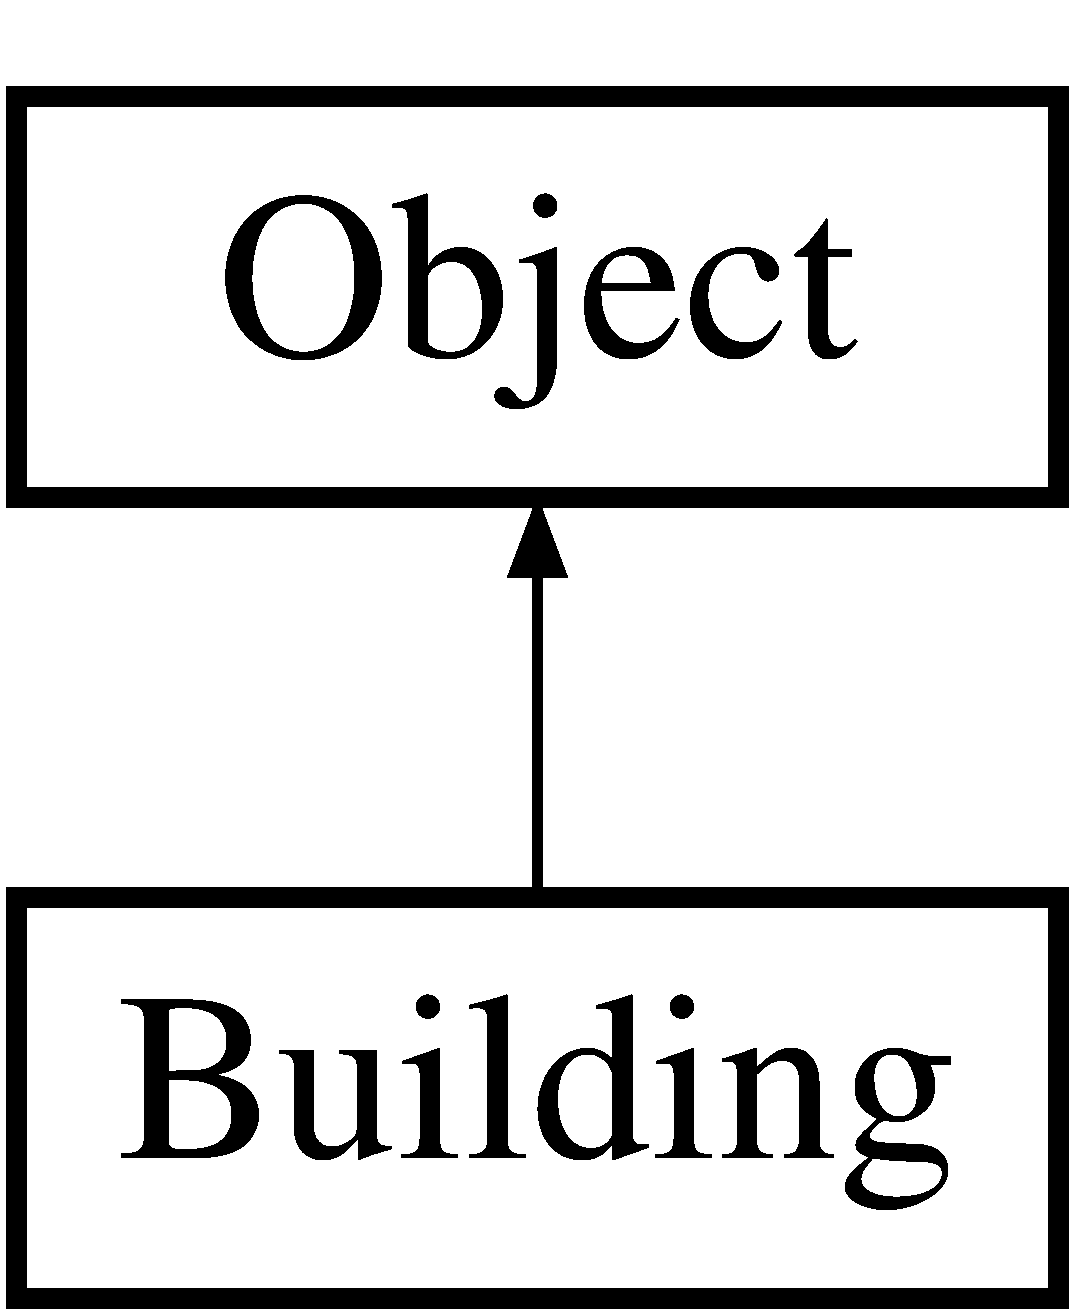
\includegraphics[height=2.000000cm]{classBuilding}
\end{center}
\end{figure}
\subsection*{Public Member Functions}
\begin{DoxyCompactItemize}
\item 
\hyperlink{classBuilding_a3db0a7481a8d811c00cc4b7f23cbc0e5}{Building} (\hyperlink{BasicTypes_8h_a91ad9478d81a7aaf2593e8d9c3d06a14}{uint} max\-\_\-space, \hyperlink{BasicTypes_8h_a91ad9478d81a7aaf2593e8d9c3d06a14}{uint} max\-\_\-health)
\begin{DoxyCompactList}\small\item\em Constructor. \end{DoxyCompactList}\item 
virtual \hyperlink{classBuilding_ab675c6a382e110b84031956cda708439}{$\sim$\-Building} ()
\begin{DoxyCompactList}\small\item\em Destructor. \end{DoxyCompactList}\item 
std\-::vector$<$ \hyperlink{classAction}{Action} $>$ $\ast$ \hyperlink{classBuilding_a2b0b464d1d8aa158729b5e2f1454ecdf}{get\-Actions} ()
\begin{DoxyCompactList}\small\item\em Gets objects pending actions. \end{DoxyCompactList}\item 
void \hyperlink{classBuilding_a5b97de4c4a379bcd8624aa2e6bfb1a3c}{decrease\-Health} (\hyperlink{BasicTypes_8h_a91ad9478d81a7aaf2593e8d9c3d06a14}{uint} delta)
\begin{DoxyCompactList}\small\item\em Decreases building's health. \end{DoxyCompactList}\item 
void \hyperlink{classBuilding_a3b373e84180fba24ba0afe981e550984}{increase\-Health} (\hyperlink{BasicTypes_8h_a91ad9478d81a7aaf2593e8d9c3d06a14}{uint} delta)
\begin{DoxyCompactList}\small\item\em Increases building's health. \end{DoxyCompactList}\item 
void \hyperlink{classBuilding_a6bb55b63a07e77ffea29316e8af400af}{damage} (\hyperlink{BasicTypes_8h_a91ad9478d81a7aaf2593e8d9c3d06a14}{uint} delta)
\begin{DoxyCompactList}\small\item\em Damages building. \end{DoxyCompactList}\item 
void \hyperlink{classBuilding_a4266475915167761e483886535382f90}{heal} (\hyperlink{BasicTypes_8h_a91ad9478d81a7aaf2593e8d9c3d06a14}{uint} delta)
\begin{DoxyCompactList}\small\item\em Repairs buidling. \end{DoxyCompactList}\item 
bool \hyperlink{classBuilding_a4c019de587cb657f2566cbb27623fc6f}{put\-Inside} (\hyperlink{classObject}{Object} $\ast$object)
\begin{DoxyCompactList}\small\item\em Puts object inside building. \end{DoxyCompactList}\item 
bool \hyperlink{classBuilding_a793d0afc39ccf187e0a749f93eecffe2}{take\-Out} (\hyperlink{classObject}{Object} $\ast$object)
\begin{DoxyCompactList}\small\item\em Takes out object from building. \end{DoxyCompactList}\item 
void \hyperlink{classBuilding_af5beff6811010a84af940243fab63041}{repair} (\hyperlink{BasicTypes_8h_a91ad9478d81a7aaf2593e8d9c3d06a14}{uint} delta)
\begin{DoxyCompactList}\small\item\em Repairs building (adds delta to building health). \end{DoxyCompactList}\item 
\hyperlink{classObjectHeap}{Object\-Heap} $\ast$ \hyperlink{classBuilding_aa2b2d6a6e7c8d55643613778fcabdd97}{get\-Contents} ()
\begin{DoxyCompactList}\small\item\em Get the value of contents. \end{DoxyCompactList}\item 
\hyperlink{BasicTypes_8h_a91ad9478d81a7aaf2593e8d9c3d06a14}{uint} \hyperlink{classBuilding_a112e8d1b75492e9cf4fef0468a64b19b}{get\-Free\-Space} ()
\begin{DoxyCompactList}\small\item\em Get the value of free\-\_\-space. \end{DoxyCompactList}\item 
\hyperlink{BasicTypes_8h_a91ad9478d81a7aaf2593e8d9c3d06a14}{uint} \hyperlink{classBuilding_ac37f23792d59ba27ba82dabe988752f6}{get\-Max\-Space} ()
\begin{DoxyCompactList}\small\item\em Get the value of max\-\_\-space. \end{DoxyCompactList}\item 
bool \hyperlink{classBuilding_a79aac1962bbd77d80fd6e1fe80abec88}{get\-Completeness} ()
\begin{DoxyCompactList}\small\item\em Get the value of is\-Finished. \end{DoxyCompactList}\end{DoxyCompactItemize}
\subsection*{Additional Inherited Members}


\subsection{Detailed Description}
\hyperlink{classBuilding}{Building} class contains information about building such as objects inside (including creatures). 

Definition at line 18 of file Building.\-h.



\subsection{Constructor \& Destructor Documentation}
\hypertarget{classBuilding_a3db0a7481a8d811c00cc4b7f23cbc0e5}{\index{Building@{Building}!Building@{Building}}
\index{Building@{Building}!Building@{Building}}
\subsubsection[{Building}]{\setlength{\rightskip}{0pt plus 5cm}Building\-::\-Building (
\begin{DoxyParamCaption}
\item[{{\bf uint}}]{max\-\_\-space, }
\item[{{\bf uint}}]{max\-\_\-health}
\end{DoxyParamCaption}
)}}\label{classBuilding_a3db0a7481a8d811c00cc4b7f23cbc0e5}


Constructor. 



Definition at line 15 of file Building.\-cpp.

\hypertarget{classBuilding_ab675c6a382e110b84031956cda708439}{\index{Building@{Building}!$\sim$\-Building@{$\sim$\-Building}}
\index{$\sim$\-Building@{$\sim$\-Building}!Building@{Building}}
\subsubsection[{$\sim$\-Building}]{\setlength{\rightskip}{0pt plus 5cm}Building\-::$\sim$\-Building (
\begin{DoxyParamCaption}
{}
\end{DoxyParamCaption}
)\hspace{0.3cm}{\ttfamily [virtual]}}}\label{classBuilding_ab675c6a382e110b84031956cda708439}


Destructor. 



Definition at line 27 of file Building.\-cpp.



\subsection{Member Function Documentation}
\hypertarget{classBuilding_a6bb55b63a07e77ffea29316e8af400af}{\index{Building@{Building}!damage@{damage}}
\index{damage@{damage}!Building@{Building}}
\subsubsection[{damage}]{\setlength{\rightskip}{0pt plus 5cm}void Building\-::damage (
\begin{DoxyParamCaption}
\item[{{\bf uint}}]{delta}
\end{DoxyParamCaption}
)\hspace{0.3cm}{\ttfamily [virtual]}}}\label{classBuilding_a6bb55b63a07e77ffea29316e8af400af}


Damages building. 


\begin{DoxyParams}{Parameters}
{\em delta} & amount of damage \\
\hline
\end{DoxyParams}


Implements \hyperlink{classObject_a816838bab5c67fce2cead6cb9122ad47}{Object}.



Definition at line 70 of file Building.\-cpp.

\hypertarget{classBuilding_a5b97de4c4a379bcd8624aa2e6bfb1a3c}{\index{Building@{Building}!decrease\-Health@{decrease\-Health}}
\index{decrease\-Health@{decrease\-Health}!Building@{Building}}
\subsubsection[{decrease\-Health}]{\setlength{\rightskip}{0pt plus 5cm}void Building\-::decrease\-Health (
\begin{DoxyParamCaption}
\item[{{\bf uint}}]{delta}
\end{DoxyParamCaption}
)}}\label{classBuilding_a5b97de4c4a379bcd8624aa2e6bfb1a3c}


Decreases building's health. 


\begin{DoxyParams}{Parameters}
{\em delta} & health to decrease \\
\hline
\end{DoxyParams}


Definition at line 46 of file Building.\-cpp.

\hypertarget{classBuilding_a2b0b464d1d8aa158729b5e2f1454ecdf}{\index{Building@{Building}!get\-Actions@{get\-Actions}}
\index{get\-Actions@{get\-Actions}!Building@{Building}}
\subsubsection[{get\-Actions}]{\setlength{\rightskip}{0pt plus 5cm}std\-::vector$<$ {\bf Action} $>$ $\ast$ Building\-::get\-Actions (
\begin{DoxyParamCaption}
{}
\end{DoxyParamCaption}
)\hspace{0.3cm}{\ttfamily [virtual]}}}\label{classBuilding_a2b0b464d1d8aa158729b5e2f1454ecdf}


Gets objects pending actions. 

\begin{DoxyReturn}{Returns}
vector with pending actions. 
\end{DoxyReturn}


Implements \hyperlink{classObject_addf0658ee2f8da579d10a6682dc097d7}{Object}.



Definition at line 36 of file Building.\-cpp.

\hypertarget{classBuilding_a79aac1962bbd77d80fd6e1fe80abec88}{\index{Building@{Building}!get\-Completeness@{get\-Completeness}}
\index{get\-Completeness@{get\-Completeness}!Building@{Building}}
\subsubsection[{get\-Completeness}]{\setlength{\rightskip}{0pt plus 5cm}bool Building\-::get\-Completeness (
\begin{DoxyParamCaption}
{}
\end{DoxyParamCaption}
)}}\label{classBuilding_a79aac1962bbd77d80fd6e1fe80abec88}


Get the value of is\-Finished. 

\begin{DoxyReturn}{Returns}
the value of is\-Finished 
\end{DoxyReturn}


Definition at line 127 of file Building.\-cpp.

\hypertarget{classBuilding_aa2b2d6a6e7c8d55643613778fcabdd97}{\index{Building@{Building}!get\-Contents@{get\-Contents}}
\index{get\-Contents@{get\-Contents}!Building@{Building}}
\subsubsection[{get\-Contents}]{\setlength{\rightskip}{0pt plus 5cm}{\bf Object\-Heap} $\ast$ Building\-::get\-Contents (
\begin{DoxyParamCaption}
{}
\end{DoxyParamCaption}
)}}\label{classBuilding_aa2b2d6a6e7c8d55643613778fcabdd97}


Get the value of contents. 

\begin{DoxyReturn}{Returns}
the value of contents 
\end{DoxyReturn}


Definition at line 112 of file Building.\-cpp.

\hypertarget{classBuilding_a112e8d1b75492e9cf4fef0468a64b19b}{\index{Building@{Building}!get\-Free\-Space@{get\-Free\-Space}}
\index{get\-Free\-Space@{get\-Free\-Space}!Building@{Building}}
\subsubsection[{get\-Free\-Space}]{\setlength{\rightskip}{0pt plus 5cm}{\bf uint} Building\-::get\-Free\-Space (
\begin{DoxyParamCaption}
{}
\end{DoxyParamCaption}
)}}\label{classBuilding_a112e8d1b75492e9cf4fef0468a64b19b}


Get the value of free\-\_\-space. 

\begin{DoxyReturn}{Returns}
the value of free\-\_\-space 
\end{DoxyReturn}


Definition at line 117 of file Building.\-cpp.

\hypertarget{classBuilding_ac37f23792d59ba27ba82dabe988752f6}{\index{Building@{Building}!get\-Max\-Space@{get\-Max\-Space}}
\index{get\-Max\-Space@{get\-Max\-Space}!Building@{Building}}
\subsubsection[{get\-Max\-Space}]{\setlength{\rightskip}{0pt plus 5cm}{\bf uint} Building\-::get\-Max\-Space (
\begin{DoxyParamCaption}
{}
\end{DoxyParamCaption}
)}}\label{classBuilding_ac37f23792d59ba27ba82dabe988752f6}


Get the value of max\-\_\-space. 

\begin{DoxyReturn}{Returns}
the value of max\-\_\-space 
\end{DoxyReturn}


Definition at line 122 of file Building.\-cpp.

\hypertarget{classBuilding_a4266475915167761e483886535382f90}{\index{Building@{Building}!heal@{heal}}
\index{heal@{heal}!Building@{Building}}
\subsubsection[{heal}]{\setlength{\rightskip}{0pt plus 5cm}void Building\-::heal (
\begin{DoxyParamCaption}
\item[{{\bf uint}}]{delta}
\end{DoxyParamCaption}
)\hspace{0.3cm}{\ttfamily [virtual]}}}\label{classBuilding_a4266475915167761e483886535382f90}


Repairs buidling. 


\begin{DoxyParams}{Parameters}
{\em delta} & amount of repairing points \\
\hline
\end{DoxyParams}


Implements \hyperlink{classObject_af7f49cb3f3c3bd9cfdbc42beecbbe5bc}{Object}.



Definition at line 75 of file Building.\-cpp.

\hypertarget{classBuilding_a3b373e84180fba24ba0afe981e550984}{\index{Building@{Building}!increase\-Health@{increase\-Health}}
\index{increase\-Health@{increase\-Health}!Building@{Building}}
\subsubsection[{increase\-Health}]{\setlength{\rightskip}{0pt plus 5cm}void Building\-::increase\-Health (
\begin{DoxyParamCaption}
\item[{{\bf uint}}]{delta}
\end{DoxyParamCaption}
)}}\label{classBuilding_a3b373e84180fba24ba0afe981e550984}


Increases building's health. 


\begin{DoxyParams}{Parameters}
{\em delta} & health to increase \\
\hline
\end{DoxyParams}


Definition at line 58 of file Building.\-cpp.

\hypertarget{classBuilding_a4c019de587cb657f2566cbb27623fc6f}{\index{Building@{Building}!put\-Inside@{put\-Inside}}
\index{put\-Inside@{put\-Inside}!Building@{Building}}
\subsubsection[{put\-Inside}]{\setlength{\rightskip}{0pt plus 5cm}bool Building\-::put\-Inside (
\begin{DoxyParamCaption}
\item[{{\bf Object} $\ast$}]{object}
\end{DoxyParamCaption}
)}}\label{classBuilding_a4c019de587cb657f2566cbb27623fc6f}


Puts object inside building. 


\begin{DoxyParams}{Parameters}
{\em object} & object to put inside \\
\hline
\end{DoxyParams}
\begin{DoxyReturn}{Returns}
success of the operation 
\end{DoxyReturn}


Definition at line 84 of file Building.\-cpp.

\hypertarget{classBuilding_af5beff6811010a84af940243fab63041}{\index{Building@{Building}!repair@{repair}}
\index{repair@{repair}!Building@{Building}}
\subsubsection[{repair}]{\setlength{\rightskip}{0pt plus 5cm}void Building\-::repair (
\begin{DoxyParamCaption}
\item[{{\bf uint}}]{delta}
\end{DoxyParamCaption}
)}}\label{classBuilding_af5beff6811010a84af940243fab63041}


Repairs building (adds delta to building health). 


\begin{DoxyParams}{Parameters}
{\em delta} & health to add \\
\hline
\end{DoxyParams}


Definition at line 98 of file Building.\-cpp.

\hypertarget{classBuilding_a793d0afc39ccf187e0a749f93eecffe2}{\index{Building@{Building}!take\-Out@{take\-Out}}
\index{take\-Out@{take\-Out}!Building@{Building}}
\subsubsection[{take\-Out}]{\setlength{\rightskip}{0pt plus 5cm}bool Building\-::take\-Out (
\begin{DoxyParamCaption}
\item[{{\bf Object} $\ast$}]{object}
\end{DoxyParamCaption}
)}}\label{classBuilding_a793d0afc39ccf187e0a749f93eecffe2}


Takes out object from building. 


\begin{DoxyParams}{Parameters}
{\em object} & object to take out \\
\hline
\end{DoxyParams}
\begin{DoxyReturn}{Returns}
success of the operation 
\end{DoxyReturn}


Definition at line 89 of file Building.\-cpp.



The documentation for this class was generated from the following files\-:\begin{DoxyCompactItemize}
\item 
model/\-World/\-Object/\-Building/\hyperlink{Building_8h}{Building.\-h}\item 
model/\-World/\-Object/\-Building/\hyperlink{Building_8cpp}{Building.\-cpp}\end{DoxyCompactItemize}

\hypertarget{classController}{\section{Controller Class Reference}
\label{classController}\index{Controller@{Controller}}
}


Class controls the world!  




{\ttfamily \#include $<$Controller.\-h$>$}

\subsection*{Public Member Functions}
\begin{DoxyCompactItemize}
\item 
\hyperlink{classController_a9cc164fbf96bbbd6bc44105824325f8e}{Controller} (\hyperlink{classWorld}{World} $\ast$world)
\begin{DoxyCompactList}\small\item\em Constructor. \end{DoxyCompactList}\item 
\hyperlink{classController_a0ab87934c4f7a266cfdb86e0f36bc1b5}{$\sim$\-Controller} ()
\begin{DoxyCompactList}\small\item\em Destructor. \end{DoxyCompactList}\item 
void \hyperlink{classController_a6fe5f85677914b59f05705bf9181d948}{step} ()
\begin{DoxyCompactList}\small\item\em Tries to make all requested actions in the world. \end{DoxyCompactList}\end{DoxyCompactItemize}


\subsection{Detailed Description}
Class controls the world! 

Definition at line 18 of file Controller.\-h.



\subsection{Constructor \& Destructor Documentation}
\hypertarget{classController_a9cc164fbf96bbbd6bc44105824325f8e}{\index{Controller@{Controller}!Controller@{Controller}}
\index{Controller@{Controller}!Controller@{Controller}}
\subsubsection[{Controller}]{\setlength{\rightskip}{0pt plus 5cm}Controller\-::\-Controller (
\begin{DoxyParamCaption}
\item[{{\bf World} $\ast$}]{world}
\end{DoxyParamCaption}
)}}\label{classController_a9cc164fbf96bbbd6bc44105824325f8e}


Constructor. 


\begin{DoxyParams}{Parameters}
{\em world} & world \\
\hline
\end{DoxyParams}


Definition at line 15 of file Controller.\-cpp.

\hypertarget{classController_a0ab87934c4f7a266cfdb86e0f36bc1b5}{\index{Controller@{Controller}!$\sim$\-Controller@{$\sim$\-Controller}}
\index{$\sim$\-Controller@{$\sim$\-Controller}!Controller@{Controller}}
\subsubsection[{$\sim$\-Controller}]{\setlength{\rightskip}{0pt plus 5cm}Controller\-::$\sim$\-Controller (
\begin{DoxyParamCaption}
{}
\end{DoxyParamCaption}
)}}\label{classController_a0ab87934c4f7a266cfdb86e0f36bc1b5}


Destructor. 



Definition at line 30 of file Controller.\-cpp.



\subsection{Member Function Documentation}
\hypertarget{classController_a6fe5f85677914b59f05705bf9181d948}{\index{Controller@{Controller}!step@{step}}
\index{step@{step}!Controller@{Controller}}
\subsubsection[{step}]{\setlength{\rightskip}{0pt plus 5cm}void Controller\-::step (
\begin{DoxyParamCaption}
{}
\end{DoxyParamCaption}
)}}\label{classController_a6fe5f85677914b59f05705bf9181d948}


Tries to make all requested actions in the world. 



Definition at line 34 of file Controller.\-cpp.



The documentation for this class was generated from the following files\-:\begin{DoxyCompactItemize}
\item 
control/\-Controller/\hyperlink{Controller_8h}{Controller.\-h}\item 
control/\-Controller/\hyperlink{Controller_8cpp}{Controller.\-cpp}\end{DoxyCompactItemize}

\hypertarget{classCreationPerformer}{\section{Creation\-Performer Class Reference}
\label{classCreationPerformer}\index{Creation\-Performer@{Creation\-Performer}}
}


Performs a creation if it is possible.  




{\ttfamily \#include $<$Creation\-Performer.\-h$>$}

Inheritance diagram for Creation\-Performer\-:\begin{figure}[H]
\begin{center}
\leavevmode
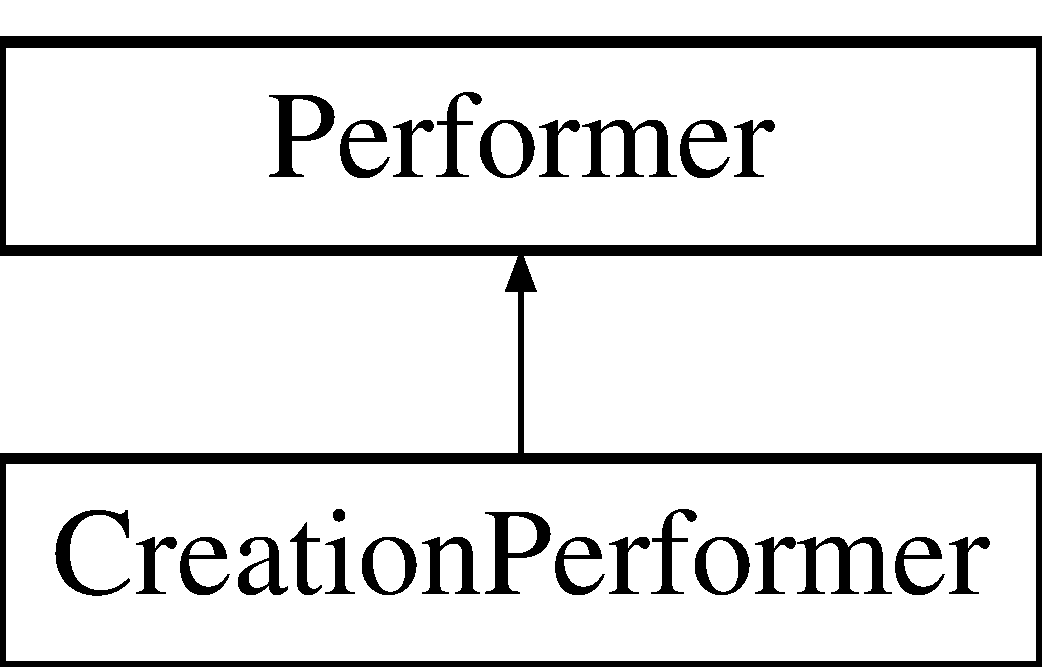
\includegraphics[height=2.000000cm]{classCreationPerformer}
\end{center}
\end{figure}
\subsection*{Public Member Functions}
\begin{DoxyCompactItemize}
\item 
\hyperlink{classCreationPerformer_a063913f6c9b6655b1fa936b1c4b418f0}{Creation\-Performer} (\hyperlink{classIndexator}{Indexator} \&indexator, \hyperlink{classWorld}{World} $\ast$world)
\begin{DoxyCompactList}\small\item\em Constructor. \end{DoxyCompactList}\item 
\hyperlink{classCreationPerformer_a7b117d6c88ab14ec084e580faf245df1}{$\sim$\-Creation\-Performer} ()
\begin{DoxyCompactList}\small\item\em Destructor. \end{DoxyCompactList}\item 
void \hyperlink{classCreationPerformer_a910e6f4c9e88fde870a4ca35e01c0173}{perform} (\hyperlink{classAction}{Action} \&action)
\begin{DoxyCompactList}\small\item\em Check if an object can create. \end{DoxyCompactList}\end{DoxyCompactItemize}


\subsection{Detailed Description}
Performs a creation if it is possible. 

Definition at line 17 of file Creation\-Performer.\-h.



\subsection{Constructor \& Destructor Documentation}
\hypertarget{classCreationPerformer_a063913f6c9b6655b1fa936b1c4b418f0}{\index{Creation\-Performer@{Creation\-Performer}!Creation\-Performer@{Creation\-Performer}}
\index{Creation\-Performer@{Creation\-Performer}!CreationPerformer@{Creation\-Performer}}
\subsubsection[{Creation\-Performer}]{\setlength{\rightskip}{0pt plus 5cm}Creation\-Performer\-::\-Creation\-Performer (
\begin{DoxyParamCaption}
\item[{{\bf Indexator} \&}]{indexator, }
\item[{{\bf World} $\ast$}]{world}
\end{DoxyParamCaption}
)}}\label{classCreationPerformer_a063913f6c9b6655b1fa936b1c4b418f0}


Constructor. 


\begin{DoxyParams}{Parameters}
{\em indexator} & indexator \\
\hline
\end{DoxyParams}


Definition at line 16 of file Creation\-Performer.\-cpp.

\hypertarget{classCreationPerformer_a7b117d6c88ab14ec084e580faf245df1}{\index{Creation\-Performer@{Creation\-Performer}!$\sim$\-Creation\-Performer@{$\sim$\-Creation\-Performer}}
\index{$\sim$\-Creation\-Performer@{$\sim$\-Creation\-Performer}!CreationPerformer@{Creation\-Performer}}
\subsubsection[{$\sim$\-Creation\-Performer}]{\setlength{\rightskip}{0pt plus 5cm}Creation\-Performer\-::$\sim$\-Creation\-Performer (
\begin{DoxyParamCaption}
{}
\end{DoxyParamCaption}
)}}\label{classCreationPerformer_a7b117d6c88ab14ec084e580faf245df1}


Destructor. 



Definition at line 23 of file Creation\-Performer.\-cpp.



\subsection{Member Function Documentation}
\hypertarget{classCreationPerformer_a910e6f4c9e88fde870a4ca35e01c0173}{\index{Creation\-Performer@{Creation\-Performer}!perform@{perform}}
\index{perform@{perform}!CreationPerformer@{Creation\-Performer}}
\subsubsection[{perform}]{\setlength{\rightskip}{0pt plus 5cm}void Creation\-Performer\-::perform (
\begin{DoxyParamCaption}
\item[{{\bf Action} \&}]{action}
\end{DoxyParamCaption}
)\hspace{0.3cm}{\ttfamily [virtual]}}}\label{classCreationPerformer_a910e6f4c9e88fde870a4ca35e01c0173}


Check if an object can create. 


\begin{DoxyParams}{Parameters}
{\em action} & a request for creation \\
\hline
\end{DoxyParams}


Implements \hyperlink{classPerformer_a4cfa828ea1f9f07fd1aa9d330adfb5d5}{Performer}.



Definition at line 28 of file Creation\-Performer.\-cpp.



The documentation for this class was generated from the following files\-:\begin{DoxyCompactItemize}
\item 
control/\-Performer/\-Creation\-Performer/\hyperlink{CreationPerformer_8h}{Creation\-Performer.\-h}\item 
control/\-Performer/\-Creation\-Performer/\hyperlink{CreationPerformer_8cpp}{Creation\-Performer.\-cpp}\end{DoxyCompactItemize}

\hypertarget{classCreature}{\section{Creature Class Reference}
\label{classCreature}\index{Creature@{Creature}}
}


Abstract \hyperlink{classCreature}{Creature} class.  




{\ttfamily \#include $<$Creature.\-h$>$}

Inheritance diagram for Creature\-:\begin{figure}[H]
\begin{center}
\leavevmode
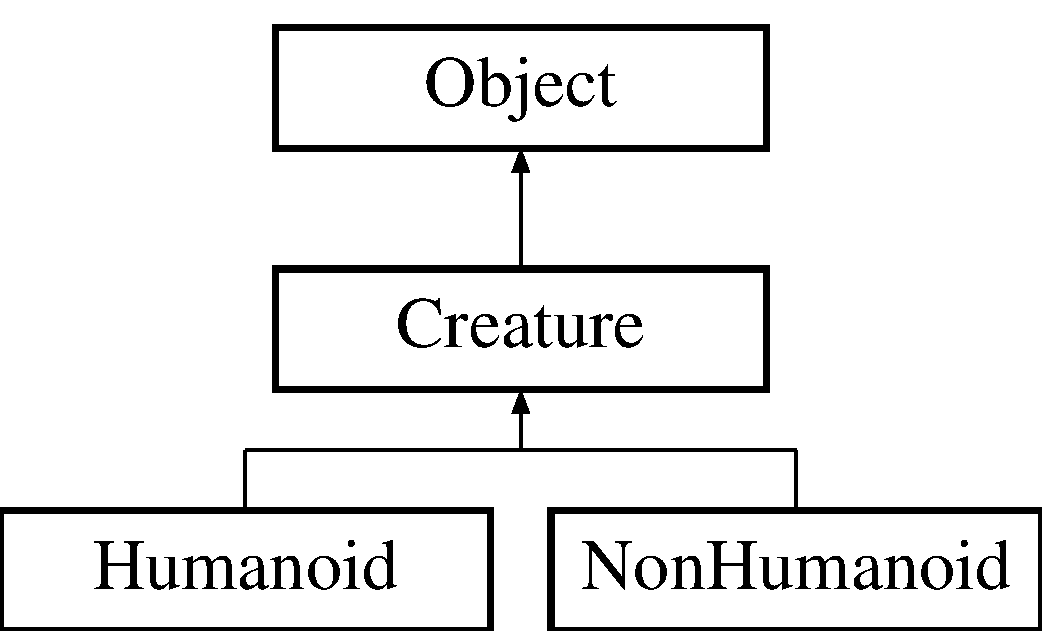
\includegraphics[height=3.000000cm]{classCreature}
\end{center}
\end{figure}
\subsection*{Public Member Functions}
\begin{DoxyCompactItemize}
\item 
\hyperlink{classCreature_a2b8a9dd1201d1142d4b634a9b6d8dfa9}{Creature} (\hyperlink{BasicTypes_8h_a5bc40f1116d89138cda8ebd1a04694df}{Creature\-Type} type, const \hyperlink{classDecisionMaker}{Decision\-Maker} \&dmaker)
\begin{DoxyCompactList}\small\item\em Random constructor (creates \hyperlink{classCreature}{Creature} with really random attributes). \end{DoxyCompactList}\item 
\hyperlink{classCreature_aa991b23f4813fbdb6f875204ed49814d}{$\sim$\-Creature} ()
\begin{DoxyCompactList}\small\item\em Destructor. \end{DoxyCompactList}\item 
void \hyperlink{classCreature_af6c61c39377198bf0426ca1929bad8a0}{set\-Window} (\hyperlink{classObjectHeap}{Object\-Heap} $\ast$window)
\begin{DoxyCompactList}\small\item\em Set the value of creature's window. \end{DoxyCompactList}\item 
\hyperlink{classObjectHeap}{Object\-Heap} $\ast$ \hyperlink{classCreature_a81d5531e518837badd23f35c8e94a302}{get\-Window} ()
\begin{DoxyCompactList}\small\item\em Get the value of creature's window. \end{DoxyCompactList}\item 
void \hyperlink{classCreature_abf1ee6a67d8dc02bc2bcf6f0a4fc2277}{set\-View\-Area} (\hyperlink{classShape}{Shape} view\-\_\-area)
\begin{DoxyCompactList}\small\item\em Set the value of view\-\_\-area. \end{DoxyCompactList}\item 
\hyperlink{classShape}{Shape} \hyperlink{classCreature_ab64257a2eb713621d3ad72ce240b14ec}{get\-View\-Area} ()
\begin{DoxyCompactList}\small\item\em Get the value of view\-\_\-area. \end{DoxyCompactList}\item 
void \hyperlink{classCreature_a218e2238145d382fb76727618db5d0d1}{set\-Age} (\hyperlink{BasicTypes_8h_a91ad9478d81a7aaf2593e8d9c3d06a14}{uint} \hyperlink{classCreature_aa3544784cbb26961f214a39b49fd171e}{age})
\begin{DoxyCompactList}\small\item\em Set the value of age. \end{DoxyCompactList}\item 
\hyperlink{BasicTypes_8h_a91ad9478d81a7aaf2593e8d9c3d06a14}{uint} \hyperlink{classCreature_a6556cd2825edd90caf6673324e5132d9}{get\-Age} ()
\begin{DoxyCompactList}\small\item\em Get the value of age. \end{DoxyCompactList}\item 
void \hyperlink{classCreature_a0182ce7212cc37901927fc9ebb26a359}{set\-Max\-Age} (\hyperlink{BasicTypes_8h_a91ad9478d81a7aaf2593e8d9c3d06a14}{uint} \hyperlink{classCreature_a57d8397db4c0e505deff7c1d7cead3e1}{max\-\_\-age})
\begin{DoxyCompactList}\small\item\em Set the value of max age. \end{DoxyCompactList}\item 
\hyperlink{BasicTypes_8h_a91ad9478d81a7aaf2593e8d9c3d06a14}{uint} \hyperlink{classCreature_a13258a0b65207bc1a283cd663485cb56}{get\-Max\-Age} ()
\begin{DoxyCompactList}\small\item\em Get the value of max age. \end{DoxyCompactList}\item 
void \hyperlink{classCreature_aaa12115f414e42efcdefff606656a47d}{set\-Health} (\hyperlink{BasicTypes_8h_a91ad9478d81a7aaf2593e8d9c3d06a14}{uint} \hyperlink{classCreature_ab59bc1917022e01b46b23f947bb8d688}{health})
\begin{DoxyCompactList}\small\item\em Set the value of health. \end{DoxyCompactList}\item 
\hyperlink{BasicTypes_8h_a91ad9478d81a7aaf2593e8d9c3d06a14}{uint} \hyperlink{classCreature_a5e75da10542de2031a67f0599f3e6427}{get\-Health} ()
\begin{DoxyCompactList}\small\item\em Get the value of health. \end{DoxyCompactList}\item 
void \hyperlink{classCreature_a3acd6ae2be4e0cc1dd3dd1b2bf539b20}{set\-Max\-Health} (\hyperlink{BasicTypes_8h_a91ad9478d81a7aaf2593e8d9c3d06a14}{uint} \hyperlink{classCreature_a0628a001b2c326388b08ea664e0c4e8f}{max\-\_\-health})
\begin{DoxyCompactList}\small\item\em Set the value of max health. \end{DoxyCompactList}\item 
\hyperlink{BasicTypes_8h_a91ad9478d81a7aaf2593e8d9c3d06a14}{uint} \hyperlink{classCreature_a769dea424947603c2fc0fc70513da83e}{get\-Max\-Health} ()
\begin{DoxyCompactList}\small\item\em Get the value of max age. \end{DoxyCompactList}\item 
\hyperlink{classObjectHeap}{Object\-Heap} $\ast$ \hyperlink{classCreature_abe4efe29a57906cd5e23c9dbf4b0bbd2}{get\-Inventory} ()
\begin{DoxyCompactList}\small\item\em Get inventory. \end{DoxyCompactList}\item 
void \hyperlink{classCreature_a5f8683a92ec95eda9abde80480e6f4a4}{decrease\-Health} (\hyperlink{BasicTypes_8h_a91ad9478d81a7aaf2593e8d9c3d06a14}{uint} delta)
\begin{DoxyCompactList}\small\item\em Decreases object's health. \end{DoxyCompactList}\item 
void \hyperlink{classCreature_a078b8ae32873d220e5701a6ee0d76d3b}{increase\-Health} (\hyperlink{BasicTypes_8h_a91ad9478d81a7aaf2593e8d9c3d06a14}{uint} delta)
\begin{DoxyCompactList}\small\item\em Increases object's health. \end{DoxyCompactList}\item 
void \hyperlink{classCreature_a6d216fa9fc5e1a70743ebc9a62dbcc01}{damage} (\hyperlink{BasicTypes_8h_a91ad9478d81a7aaf2593e8d9c3d06a14}{uint} delta)
\begin{DoxyCompactList}\small\item\em Damages creature. \end{DoxyCompactList}\item 
void \hyperlink{classCreature_ab168ec8b1230205eb0dda7edbef60469}{heal} (\hyperlink{BasicTypes_8h_a91ad9478d81a7aaf2593e8d9c3d06a14}{uint} delta)
\begin{DoxyCompactList}\small\item\em Heals creature. \end{DoxyCompactList}\end{DoxyCompactItemize}
\subsection*{Protected Member Functions}
\begin{DoxyCompactItemize}
\item 
virtual void \hyperlink{classCreature_a2f60a8f7e8c9432b3c91d91fbea6eb86}{update\-Age} ()=0
\begin{DoxyCompactList}\small\item\em Updates age. \end{DoxyCompactList}\item 
virtual void \hyperlink{classCreature_aa7e689cd7024701857bc069a8b1c3959}{update\-Need\-In\-Desc} ()=0
\begin{DoxyCompactList}\small\item\em Updates need\-\_\-in\-\_\-descendants. \end{DoxyCompactList}\item 
virtual void \hyperlink{classCreature_aa070b3e571a6f0ace18ac4774637e985}{update\-Safety} ()=0
\begin{DoxyCompactList}\small\item\em Updates safety. \end{DoxyCompactList}\item 
virtual void \hyperlink{classCreature_adc200567e6af258a7f6f1be4fbe029bc}{update\-Common\-Attrs} ()=0
\begin{DoxyCompactList}\small\item\em Updates hunger, sleepiness, health. \end{DoxyCompactList}\end{DoxyCompactItemize}
\subsection*{Protected Attributes}
\begin{DoxyCompactItemize}
\item 
\hyperlink{BasicTypes_8h_a5303344c79577371e13252b373606706}{Creature\-Action} \hyperlink{classCreature_a3f97c007c64aa78502e9fa9cab716408}{current\-\_\-action}
\begin{DoxyCompactList}\small\item\em Current creature's action. \end{DoxyCompactList}\item 
\hyperlink{classObjectHeap}{Object\-Heap} $\ast$ \hyperlink{classCreature_a2941f1bf4753c4cc196ca7b20ade706c}{objects\-\_\-around}
\begin{DoxyCompactList}\small\item\em \hyperlink{classCreature}{Creature}'s enviroment. \end{DoxyCompactList}\item 
arma\-::mat \hyperlink{classCreature_a641e41105d04d3faf56ca7a0132586e2}{attrs}
\begin{DoxyCompactList}\small\item\em Matrix of attributes. \end{DoxyCompactList}\item 
const \hyperlink{classDecisionMaker}{Decision\-Maker} \& \hyperlink{classCreature_a8499febfbaad5783181a01000cbc4dc6}{brains}
\begin{DoxyCompactList}\small\item\em Reference to creature's \hyperlink{classDecisionMaker}{Decision\-Maker}. \end{DoxyCompactList}\item 
\hyperlink{BasicTypes_8h_a91ad9478d81a7aaf2593e8d9c3d06a14}{uint} \hyperlink{classCreature_aa3544784cbb26961f214a39b49fd171e}{age}
\begin{DoxyCompactList}\small\item\em Current age. \end{DoxyCompactList}\item 
\hyperlink{BasicTypes_8h_a91ad9478d81a7aaf2593e8d9c3d06a14}{uint} \hyperlink{classCreature_a57d8397db4c0e505deff7c1d7cead3e1}{max\-\_\-age}
\begin{DoxyCompactList}\small\item\em Maximum possible age. \end{DoxyCompactList}\item 
\hyperlink{BasicTypes_8h_a91ad9478d81a7aaf2593e8d9c3d06a14}{uint} \hyperlink{classCreature_ab59bc1917022e01b46b23f947bb8d688}{health}
\begin{DoxyCompactList}\small\item\em Current health. \end{DoxyCompactList}\item 
\hyperlink{BasicTypes_8h_a91ad9478d81a7aaf2593e8d9c3d06a14}{uint} \hyperlink{classCreature_a0628a001b2c326388b08ea664e0c4e8f}{max\-\_\-health}
\begin{DoxyCompactList}\small\item\em Maximum possible health. \end{DoxyCompactList}\item 
\hyperlink{BasicTypes_8h_a91ad9478d81a7aaf2593e8d9c3d06a14}{uint} \hyperlink{classCreature_a3f6c69d85deb3a91a823913e67f19709}{sleepiness}
\begin{DoxyCompactList}\small\item\em Current value of sleepiness. \end{DoxyCompactList}\item 
\hyperlink{BasicTypes_8h_a91ad9478d81a7aaf2593e8d9c3d06a14}{uint} \hyperlink{classCreature_ae52439324e6404f73bf0e316fdf5a31b}{max\-\_\-sleepiness}
\begin{DoxyCompactList}\small\item\em Maximum possible value of sleepiness. \end{DoxyCompactList}\item 
\hyperlink{BasicTypes_8h_a91ad9478d81a7aaf2593e8d9c3d06a14}{uint} \hyperlink{classCreature_aed2975e3833046d705ae928dc2aed4b6}{need\-\_\-in\-\_\-descendants}
\begin{DoxyCompactList}\small\item\em Current value of need\-\_\-in\-\_\-descendants (0-\/100) \end{DoxyCompactList}\item 
\hyperlink{BasicTypes_8h_a91ad9478d81a7aaf2593e8d9c3d06a14}{uint} \hyperlink{classCreature_a898df2aff71e6908209969eea863ccf8}{safety}
\begin{DoxyCompactList}\small\item\em Current safety. \end{DoxyCompactList}\item 
\hyperlink{BasicTypes_8h_a91ad9478d81a7aaf2593e8d9c3d06a14}{uint} \hyperlink{classCreature_a0ac52285317bd2d52b3901b9c2a9c24a}{hunger}
\begin{DoxyCompactList}\small\item\em Current value of hunger. \end{DoxyCompactList}\item 
\hyperlink{BasicTypes_8h_a91ad9478d81a7aaf2593e8d9c3d06a14}{uint} \hyperlink{classCreature_a49691e6b47ba6704b980963ab63c1881}{max\-\_\-hunger}
\begin{DoxyCompactList}\small\item\em Maximum possible value of hunger. \end{DoxyCompactList}\item 
\hyperlink{BasicTypes_8h_a91ad9478d81a7aaf2593e8d9c3d06a14}{uint} \hyperlink{classCreature_aa1c351d6da7f1df976efb27fe21d5014}{common\-\_\-steps}
\begin{DoxyCompactList}\small\item\em Amount for steps to common update. \end{DoxyCompactList}\item 
\hyperlink{BasicTypes_8h_a91ad9478d81a7aaf2593e8d9c3d06a14}{uint} \hyperlink{classCreature_aa9bf4d151801ecb1326cd734b341167d}{age\-\_\-steps}
\begin{DoxyCompactList}\small\item\em Amount for steps to age update. \end{DoxyCompactList}\item 
\hyperlink{BasicTypes_8h_a91ad9478d81a7aaf2593e8d9c3d06a14}{uint} \hyperlink{classCreature_ad80371401e4349fd4c5b05367964b530}{desc\-\_\-steps}
\begin{DoxyCompactList}\small\item\em Amount for steps to need\-\_\-in\-\_\-descendant update. \end{DoxyCompactList}\item 
\hyperlink{BasicTypes_8h_a91ad9478d81a7aaf2593e8d9c3d06a14}{uint} \hyperlink{classCreature_a0781a2fc0015b162482cc3f92aae3ec8}{safety\-\_\-steps}
\begin{DoxyCompactList}\small\item\em Amount for steps to safety update. \end{DoxyCompactList}\end{DoxyCompactItemize}


\subsection{Detailed Description}
Abstract \hyperlink{classCreature}{Creature} class. 

Definition at line 18 of file Creature.\-h.



\subsection{Constructor \& Destructor Documentation}
\hypertarget{classCreature_a2b8a9dd1201d1142d4b634a9b6d8dfa9}{\index{Creature@{Creature}!Creature@{Creature}}
\index{Creature@{Creature}!Creature@{Creature}}
\subsubsection[{Creature}]{\setlength{\rightskip}{0pt plus 5cm}Creature\-::\-Creature (
\begin{DoxyParamCaption}
\item[{{\bf Creature\-Type}}]{type, }
\item[{const {\bf Decision\-Maker} \&}]{dmaker}
\end{DoxyParamCaption}
)}}\label{classCreature_a2b8a9dd1201d1142d4b634a9b6d8dfa9}


Random constructor (creates \hyperlink{classCreature}{Creature} with really random attributes). 


\begin{DoxyParams}{Parameters}
{\em type} & creature's type \\
\hline
{\em dmaker} & creature's decision maker \\
\hline
\end{DoxyParams}


Definition at line 15 of file Creature.\-cpp.

\hypertarget{classCreature_aa991b23f4813fbdb6f875204ed49814d}{\index{Creature@{Creature}!$\sim$\-Creature@{$\sim$\-Creature}}
\index{$\sim$\-Creature@{$\sim$\-Creature}!Creature@{Creature}}
\subsubsection[{$\sim$\-Creature}]{\setlength{\rightskip}{0pt plus 5cm}Creature\-::$\sim$\-Creature (
\begin{DoxyParamCaption}
{}
\end{DoxyParamCaption}
)}}\label{classCreature_aa991b23f4813fbdb6f875204ed49814d}


Destructor. 



Definition at line 39 of file Creature.\-cpp.



\subsection{Member Function Documentation}
\hypertarget{classCreature_a6d216fa9fc5e1a70743ebc9a62dbcc01}{\index{Creature@{Creature}!damage@{damage}}
\index{damage@{damage}!Creature@{Creature}}
\subsubsection[{damage}]{\setlength{\rightskip}{0pt plus 5cm}void Creature\-::damage (
\begin{DoxyParamCaption}
\item[{{\bf uint}}]{delta}
\end{DoxyParamCaption}
)\hspace{0.3cm}{\ttfamily [virtual]}}}\label{classCreature_a6d216fa9fc5e1a70743ebc9a62dbcc01}


Damages creature. 


\begin{DoxyParams}{Parameters}
{\em delta} & amount of damage \\
\hline
\end{DoxyParams}


Implements \hyperlink{classObject_a816838bab5c67fce2cead6cb9122ad47}{Object}.



Definition at line 142 of file Creature.\-cpp.

\hypertarget{classCreature_a5f8683a92ec95eda9abde80480e6f4a4}{\index{Creature@{Creature}!decrease\-Health@{decrease\-Health}}
\index{decrease\-Health@{decrease\-Health}!Creature@{Creature}}
\subsubsection[{decrease\-Health}]{\setlength{\rightskip}{0pt plus 5cm}void Creature\-::decrease\-Health (
\begin{DoxyParamCaption}
\item[{{\bf uint}}]{delta}
\end{DoxyParamCaption}
)}}\label{classCreature_a5f8683a92ec95eda9abde80480e6f4a4}


Decreases object's health. 


\begin{DoxyParams}{Parameters}
{\em delta} & health to decrease \\
\hline
\end{DoxyParams}


Definition at line 118 of file Creature.\-cpp.

\hypertarget{classCreature_a6556cd2825edd90caf6673324e5132d9}{\index{Creature@{Creature}!get\-Age@{get\-Age}}
\index{get\-Age@{get\-Age}!Creature@{Creature}}
\subsubsection[{get\-Age}]{\setlength{\rightskip}{0pt plus 5cm}{\bf uint} Creature\-::get\-Age (
\begin{DoxyParamCaption}
{}
\end{DoxyParamCaption}
)}}\label{classCreature_a6556cd2825edd90caf6673324e5132d9}


Get the value of age. 

\begin{DoxyReturn}{Returns}
the value of age 
\end{DoxyReturn}


Definition at line 73 of file Creature.\-cpp.

\hypertarget{classCreature_a5e75da10542de2031a67f0599f3e6427}{\index{Creature@{Creature}!get\-Health@{get\-Health}}
\index{get\-Health@{get\-Health}!Creature@{Creature}}
\subsubsection[{get\-Health}]{\setlength{\rightskip}{0pt plus 5cm}{\bf uint} Creature\-::get\-Health (
\begin{DoxyParamCaption}
{}
\end{DoxyParamCaption}
)}}\label{classCreature_a5e75da10542de2031a67f0599f3e6427}


Get the value of health. 

\begin{DoxyReturn}{Returns}
the value of health 
\end{DoxyReturn}


Definition at line 94 of file Creature.\-cpp.

\hypertarget{classCreature_abe4efe29a57906cd5e23c9dbf4b0bbd2}{\index{Creature@{Creature}!get\-Inventory@{get\-Inventory}}
\index{get\-Inventory@{get\-Inventory}!Creature@{Creature}}
\subsubsection[{get\-Inventory}]{\setlength{\rightskip}{0pt plus 5cm}{\bf Object\-Heap} $\ast$ Creature\-::get\-Inventory (
\begin{DoxyParamCaption}
{}
\end{DoxyParamCaption}
)}}\label{classCreature_abe4efe29a57906cd5e23c9dbf4b0bbd2}


Get inventory. 

\begin{DoxyReturn}{Returns}
inventory 
\end{DoxyReturn}


Definition at line 109 of file Creature.\-cpp.

\hypertarget{classCreature_a13258a0b65207bc1a283cd663485cb56}{\index{Creature@{Creature}!get\-Max\-Age@{get\-Max\-Age}}
\index{get\-Max\-Age@{get\-Max\-Age}!Creature@{Creature}}
\subsubsection[{get\-Max\-Age}]{\setlength{\rightskip}{0pt plus 5cm}{\bf uint} Creature\-::get\-Max\-Age (
\begin{DoxyParamCaption}
{}
\end{DoxyParamCaption}
)}}\label{classCreature_a13258a0b65207bc1a283cd663485cb56}


Get the value of max age. 

\begin{DoxyReturn}{Returns}
the value of max age 
\end{DoxyReturn}


Definition at line 83 of file Creature.\-cpp.

\hypertarget{classCreature_a769dea424947603c2fc0fc70513da83e}{\index{Creature@{Creature}!get\-Max\-Health@{get\-Max\-Health}}
\index{get\-Max\-Health@{get\-Max\-Health}!Creature@{Creature}}
\subsubsection[{get\-Max\-Health}]{\setlength{\rightskip}{0pt plus 5cm}{\bf uint} Creature\-::get\-Max\-Health (
\begin{DoxyParamCaption}
{}
\end{DoxyParamCaption}
)}}\label{classCreature_a769dea424947603c2fc0fc70513da83e}


Get the value of max age. 

\begin{DoxyReturn}{Returns}
the value of max age 
\end{DoxyReturn}


Definition at line 104 of file Creature.\-cpp.

\hypertarget{classCreature_ab64257a2eb713621d3ad72ce240b14ec}{\index{Creature@{Creature}!get\-View\-Area@{get\-View\-Area}}
\index{get\-View\-Area@{get\-View\-Area}!Creature@{Creature}}
\subsubsection[{get\-View\-Area}]{\setlength{\rightskip}{0pt plus 5cm}{\bf Shape} Creature\-::get\-View\-Area (
\begin{DoxyParamCaption}
{}
\end{DoxyParamCaption}
)}}\label{classCreature_ab64257a2eb713621d3ad72ce240b14ec}


Get the value of view\-\_\-area. 

\begin{DoxyReturn}{Returns}
the value of view\-\_\-area 
\end{DoxyReturn}


Definition at line 63 of file Creature.\-cpp.

\hypertarget{classCreature_a81d5531e518837badd23f35c8e94a302}{\index{Creature@{Creature}!get\-Window@{get\-Window}}
\index{get\-Window@{get\-Window}!Creature@{Creature}}
\subsubsection[{get\-Window}]{\setlength{\rightskip}{0pt plus 5cm}{\bf Object\-Heap} $\ast$ Creature\-::get\-Window (
\begin{DoxyParamCaption}
{}
\end{DoxyParamCaption}
)}}\label{classCreature_a81d5531e518837badd23f35c8e94a302}


Get the value of creature's window. 

\begin{DoxyReturn}{Returns}
the window 
\end{DoxyReturn}


Definition at line 53 of file Creature.\-cpp.

\hypertarget{classCreature_ab168ec8b1230205eb0dda7edbef60469}{\index{Creature@{Creature}!heal@{heal}}
\index{heal@{heal}!Creature@{Creature}}
\subsubsection[{heal}]{\setlength{\rightskip}{0pt plus 5cm}void Creature\-::heal (
\begin{DoxyParamCaption}
\item[{{\bf uint}}]{delta}
\end{DoxyParamCaption}
)\hspace{0.3cm}{\ttfamily [virtual]}}}\label{classCreature_ab168ec8b1230205eb0dda7edbef60469}


Heals creature. 


\begin{DoxyParams}{Parameters}
{\em delta} & amount of healing points \\
\hline
\end{DoxyParams}


Implements \hyperlink{classObject_af7f49cb3f3c3bd9cfdbc42beecbbe5bc}{Object}.



Definition at line 147 of file Creature.\-cpp.

\hypertarget{classCreature_a078b8ae32873d220e5701a6ee0d76d3b}{\index{Creature@{Creature}!increase\-Health@{increase\-Health}}
\index{increase\-Health@{increase\-Health}!Creature@{Creature}}
\subsubsection[{increase\-Health}]{\setlength{\rightskip}{0pt plus 5cm}void Creature\-::increase\-Health (
\begin{DoxyParamCaption}
\item[{{\bf uint}}]{delta}
\end{DoxyParamCaption}
)}}\label{classCreature_a078b8ae32873d220e5701a6ee0d76d3b}


Increases object's health. 


\begin{DoxyParams}{Parameters}
{\em delta} & health to increase \\
\hline
\end{DoxyParams}


Definition at line 130 of file Creature.\-cpp.

\hypertarget{classCreature_a218e2238145d382fb76727618db5d0d1}{\index{Creature@{Creature}!set\-Age@{set\-Age}}
\index{set\-Age@{set\-Age}!Creature@{Creature}}
\subsubsection[{set\-Age}]{\setlength{\rightskip}{0pt plus 5cm}void Creature\-::set\-Age (
\begin{DoxyParamCaption}
\item[{{\bf uint}}]{age}
\end{DoxyParamCaption}
)}}\label{classCreature_a218e2238145d382fb76727618db5d0d1}


Set the value of age. 


\begin{DoxyParams}{Parameters}
{\em age} & new value of age \\
\hline
\end{DoxyParams}


Definition at line 68 of file Creature.\-cpp.

\hypertarget{classCreature_aaa12115f414e42efcdefff606656a47d}{\index{Creature@{Creature}!set\-Health@{set\-Health}}
\index{set\-Health@{set\-Health}!Creature@{Creature}}
\subsubsection[{set\-Health}]{\setlength{\rightskip}{0pt plus 5cm}void Creature\-::set\-Health (
\begin{DoxyParamCaption}
\item[{{\bf uint}}]{health}
\end{DoxyParamCaption}
)}}\label{classCreature_aaa12115f414e42efcdefff606656a47d}


Set the value of health. 


\begin{DoxyParams}{Parameters}
{\em health} & new value of health \\
\hline
\end{DoxyParams}


Definition at line 89 of file Creature.\-cpp.

\hypertarget{classCreature_a0182ce7212cc37901927fc9ebb26a359}{\index{Creature@{Creature}!set\-Max\-Age@{set\-Max\-Age}}
\index{set\-Max\-Age@{set\-Max\-Age}!Creature@{Creature}}
\subsubsection[{set\-Max\-Age}]{\setlength{\rightskip}{0pt plus 5cm}void Creature\-::set\-Max\-Age (
\begin{DoxyParamCaption}
\item[{{\bf uint}}]{max\-\_\-age}
\end{DoxyParamCaption}
)}}\label{classCreature_a0182ce7212cc37901927fc9ebb26a359}


Set the value of max age. 


\begin{DoxyParams}{Parameters}
{\em max\-\_\-age} & new value of max age \\
\hline
\end{DoxyParams}


Definition at line 78 of file Creature.\-cpp.

\hypertarget{classCreature_a3acd6ae2be4e0cc1dd3dd1b2bf539b20}{\index{Creature@{Creature}!set\-Max\-Health@{set\-Max\-Health}}
\index{set\-Max\-Health@{set\-Max\-Health}!Creature@{Creature}}
\subsubsection[{set\-Max\-Health}]{\setlength{\rightskip}{0pt plus 5cm}void Creature\-::set\-Max\-Health (
\begin{DoxyParamCaption}
\item[{{\bf uint}}]{max\-\_\-health}
\end{DoxyParamCaption}
)}}\label{classCreature_a3acd6ae2be4e0cc1dd3dd1b2bf539b20}


Set the value of max health. 


\begin{DoxyParams}{Parameters}
{\em max\-\_\-health} & new value of max health \\
\hline
\end{DoxyParams}


Definition at line 99 of file Creature.\-cpp.

\hypertarget{classCreature_abf1ee6a67d8dc02bc2bcf6f0a4fc2277}{\index{Creature@{Creature}!set\-View\-Area@{set\-View\-Area}}
\index{set\-View\-Area@{set\-View\-Area}!Creature@{Creature}}
\subsubsection[{set\-View\-Area}]{\setlength{\rightskip}{0pt plus 5cm}void Creature\-::set\-View\-Area (
\begin{DoxyParamCaption}
\item[{{\bf Shape}}]{view\-\_\-area}
\end{DoxyParamCaption}
)}}\label{classCreature_abf1ee6a67d8dc02bc2bcf6f0a4fc2277}


Set the value of view\-\_\-area. 


\begin{DoxyParams}{Parameters}
{\em view\-\_\-area} & the new value of view\-\_\-area \\
\hline
\end{DoxyParams}


Definition at line 58 of file Creature.\-cpp.

\hypertarget{classCreature_af6c61c39377198bf0426ca1929bad8a0}{\index{Creature@{Creature}!set\-Window@{set\-Window}}
\index{set\-Window@{set\-Window}!Creature@{Creature}}
\subsubsection[{set\-Window}]{\setlength{\rightskip}{0pt plus 5cm}void Creature\-::set\-Window (
\begin{DoxyParamCaption}
\item[{{\bf Object\-Heap} $\ast$}]{window}
\end{DoxyParamCaption}
)}}\label{classCreature_af6c61c39377198bf0426ca1929bad8a0}


Set the value of creature's window. 


\begin{DoxyParams}{Parameters}
{\em window} & the new value of window \\
\hline
\end{DoxyParams}


Definition at line 48 of file Creature.\-cpp.

\hypertarget{classCreature_a2f60a8f7e8c9432b3c91d91fbea6eb86}{\index{Creature@{Creature}!update\-Age@{update\-Age}}
\index{update\-Age@{update\-Age}!Creature@{Creature}}
\subsubsection[{update\-Age}]{\setlength{\rightskip}{0pt plus 5cm}virtual void Creature\-::update\-Age (
\begin{DoxyParamCaption}
{}
\end{DoxyParamCaption}
)\hspace{0.3cm}{\ttfamily [protected]}, {\ttfamily [pure virtual]}}}\label{classCreature_a2f60a8f7e8c9432b3c91d91fbea6eb86}


Updates age. 

\hypertarget{classCreature_adc200567e6af258a7f6f1be4fbe029bc}{\index{Creature@{Creature}!update\-Common\-Attrs@{update\-Common\-Attrs}}
\index{update\-Common\-Attrs@{update\-Common\-Attrs}!Creature@{Creature}}
\subsubsection[{update\-Common\-Attrs}]{\setlength{\rightskip}{0pt plus 5cm}virtual void Creature\-::update\-Common\-Attrs (
\begin{DoxyParamCaption}
{}
\end{DoxyParamCaption}
)\hspace{0.3cm}{\ttfamily [protected]}, {\ttfamily [pure virtual]}}}\label{classCreature_adc200567e6af258a7f6f1be4fbe029bc}


Updates hunger, sleepiness, health. 

\hypertarget{classCreature_aa7e689cd7024701857bc069a8b1c3959}{\index{Creature@{Creature}!update\-Need\-In\-Desc@{update\-Need\-In\-Desc}}
\index{update\-Need\-In\-Desc@{update\-Need\-In\-Desc}!Creature@{Creature}}
\subsubsection[{update\-Need\-In\-Desc}]{\setlength{\rightskip}{0pt plus 5cm}virtual void Creature\-::update\-Need\-In\-Desc (
\begin{DoxyParamCaption}
{}
\end{DoxyParamCaption}
)\hspace{0.3cm}{\ttfamily [protected]}, {\ttfamily [pure virtual]}}}\label{classCreature_aa7e689cd7024701857bc069a8b1c3959}


Updates need\-\_\-in\-\_\-descendants. 

\hypertarget{classCreature_aa070b3e571a6f0ace18ac4774637e985}{\index{Creature@{Creature}!update\-Safety@{update\-Safety}}
\index{update\-Safety@{update\-Safety}!Creature@{Creature}}
\subsubsection[{update\-Safety}]{\setlength{\rightskip}{0pt plus 5cm}virtual void Creature\-::update\-Safety (
\begin{DoxyParamCaption}
{}
\end{DoxyParamCaption}
)\hspace{0.3cm}{\ttfamily [protected]}, {\ttfamily [pure virtual]}}}\label{classCreature_aa070b3e571a6f0ace18ac4774637e985}


Updates safety. 



\subsection{Member Data Documentation}
\hypertarget{classCreature_aa3544784cbb26961f214a39b49fd171e}{\index{Creature@{Creature}!age@{age}}
\index{age@{age}!Creature@{Creature}}
\subsubsection[{age}]{\setlength{\rightskip}{0pt plus 5cm}{\bf uint} Creature\-::age\hspace{0.3cm}{\ttfamily [protected]}}}\label{classCreature_aa3544784cbb26961f214a39b49fd171e}


Current age. 



Definition at line 174 of file Creature.\-h.

\hypertarget{classCreature_aa9bf4d151801ecb1326cd734b341167d}{\index{Creature@{Creature}!age\-\_\-steps@{age\-\_\-steps}}
\index{age\-\_\-steps@{age\-\_\-steps}!Creature@{Creature}}
\subsubsection[{age\-\_\-steps}]{\setlength{\rightskip}{0pt plus 5cm}{\bf uint} Creature\-::age\-\_\-steps\hspace{0.3cm}{\ttfamily [protected]}}}\label{classCreature_aa9bf4d151801ecb1326cd734b341167d}


Amount for steps to age update. 



Definition at line 208 of file Creature.\-h.

\hypertarget{classCreature_a641e41105d04d3faf56ca7a0132586e2}{\index{Creature@{Creature}!attrs@{attrs}}
\index{attrs@{attrs}!Creature@{Creature}}
\subsubsection[{attrs}]{\setlength{\rightskip}{0pt plus 5cm}arma\-::mat Creature\-::attrs\hspace{0.3cm}{\ttfamily [protected]}}}\label{classCreature_a641e41105d04d3faf56ca7a0132586e2}


Matrix of attributes. 



Definition at line 168 of file Creature.\-h.

\hypertarget{classCreature_a8499febfbaad5783181a01000cbc4dc6}{\index{Creature@{Creature}!brains@{brains}}
\index{brains@{brains}!Creature@{Creature}}
\subsubsection[{brains}]{\setlength{\rightskip}{0pt plus 5cm}const {\bf Decision\-Maker}\& Creature\-::brains\hspace{0.3cm}{\ttfamily [protected]}}}\label{classCreature_a8499febfbaad5783181a01000cbc4dc6}


Reference to creature's \hyperlink{classDecisionMaker}{Decision\-Maker}. 



Definition at line 171 of file Creature.\-h.

\hypertarget{classCreature_aa1c351d6da7f1df976efb27fe21d5014}{\index{Creature@{Creature}!common\-\_\-steps@{common\-\_\-steps}}
\index{common\-\_\-steps@{common\-\_\-steps}!Creature@{Creature}}
\subsubsection[{common\-\_\-steps}]{\setlength{\rightskip}{0pt plus 5cm}{\bf uint} Creature\-::common\-\_\-steps\hspace{0.3cm}{\ttfamily [protected]}}}\label{classCreature_aa1c351d6da7f1df976efb27fe21d5014}


Amount for steps to common update. 



Definition at line 206 of file Creature.\-h.

\hypertarget{classCreature_a3f97c007c64aa78502e9fa9cab716408}{\index{Creature@{Creature}!current\-\_\-action@{current\-\_\-action}}
\index{current\-\_\-action@{current\-\_\-action}!Creature@{Creature}}
\subsubsection[{current\-\_\-action}]{\setlength{\rightskip}{0pt plus 5cm}{\bf Creature\-Action} Creature\-::current\-\_\-action\hspace{0.3cm}{\ttfamily [protected]}}}\label{classCreature_a3f97c007c64aa78502e9fa9cab716408}


Current creature's action. 



Definition at line 163 of file Creature.\-h.

\hypertarget{classCreature_ad80371401e4349fd4c5b05367964b530}{\index{Creature@{Creature}!desc\-\_\-steps@{desc\-\_\-steps}}
\index{desc\-\_\-steps@{desc\-\_\-steps}!Creature@{Creature}}
\subsubsection[{desc\-\_\-steps}]{\setlength{\rightskip}{0pt plus 5cm}{\bf uint} Creature\-::desc\-\_\-steps\hspace{0.3cm}{\ttfamily [protected]}}}\label{classCreature_ad80371401e4349fd4c5b05367964b530}


Amount for steps to need\-\_\-in\-\_\-descendant update. 



Definition at line 210 of file Creature.\-h.

\hypertarget{classCreature_ab59bc1917022e01b46b23f947bb8d688}{\index{Creature@{Creature}!health@{health}}
\index{health@{health}!Creature@{Creature}}
\subsubsection[{health}]{\setlength{\rightskip}{0pt plus 5cm}{\bf uint} Creature\-::health\hspace{0.3cm}{\ttfamily [protected]}}}\label{classCreature_ab59bc1917022e01b46b23f947bb8d688}


Current health. 



Definition at line 180 of file Creature.\-h.

\hypertarget{classCreature_a0ac52285317bd2d52b3901b9c2a9c24a}{\index{Creature@{Creature}!hunger@{hunger}}
\index{hunger@{hunger}!Creature@{Creature}}
\subsubsection[{hunger}]{\setlength{\rightskip}{0pt plus 5cm}{\bf uint} Creature\-::hunger\hspace{0.3cm}{\ttfamily [protected]}}}\label{classCreature_a0ac52285317bd2d52b3901b9c2a9c24a}


Current value of hunger. 



Definition at line 201 of file Creature.\-h.

\hypertarget{classCreature_a57d8397db4c0e505deff7c1d7cead3e1}{\index{Creature@{Creature}!max\-\_\-age@{max\-\_\-age}}
\index{max\-\_\-age@{max\-\_\-age}!Creature@{Creature}}
\subsubsection[{max\-\_\-age}]{\setlength{\rightskip}{0pt plus 5cm}{\bf uint} Creature\-::max\-\_\-age\hspace{0.3cm}{\ttfamily [protected]}}}\label{classCreature_a57d8397db4c0e505deff7c1d7cead3e1}


Maximum possible age. 



Definition at line 177 of file Creature.\-h.

\hypertarget{classCreature_a0628a001b2c326388b08ea664e0c4e8f}{\index{Creature@{Creature}!max\-\_\-health@{max\-\_\-health}}
\index{max\-\_\-health@{max\-\_\-health}!Creature@{Creature}}
\subsubsection[{max\-\_\-health}]{\setlength{\rightskip}{0pt plus 5cm}{\bf uint} Creature\-::max\-\_\-health\hspace{0.3cm}{\ttfamily [protected]}}}\label{classCreature_a0628a001b2c326388b08ea664e0c4e8f}


Maximum possible health. 



Definition at line 183 of file Creature.\-h.

\hypertarget{classCreature_a49691e6b47ba6704b980963ab63c1881}{\index{Creature@{Creature}!max\-\_\-hunger@{max\-\_\-hunger}}
\index{max\-\_\-hunger@{max\-\_\-hunger}!Creature@{Creature}}
\subsubsection[{max\-\_\-hunger}]{\setlength{\rightskip}{0pt plus 5cm}{\bf uint} Creature\-::max\-\_\-hunger\hspace{0.3cm}{\ttfamily [protected]}}}\label{classCreature_a49691e6b47ba6704b980963ab63c1881}


Maximum possible value of hunger. 



Definition at line 203 of file Creature.\-h.

\hypertarget{classCreature_ae52439324e6404f73bf0e316fdf5a31b}{\index{Creature@{Creature}!max\-\_\-sleepiness@{max\-\_\-sleepiness}}
\index{max\-\_\-sleepiness@{max\-\_\-sleepiness}!Creature@{Creature}}
\subsubsection[{max\-\_\-sleepiness}]{\setlength{\rightskip}{0pt plus 5cm}{\bf uint} Creature\-::max\-\_\-sleepiness\hspace{0.3cm}{\ttfamily [protected]}}}\label{classCreature_ae52439324e6404f73bf0e316fdf5a31b}


Maximum possible value of sleepiness. 



Definition at line 190 of file Creature.\-h.

\hypertarget{classCreature_aed2975e3833046d705ae928dc2aed4b6}{\index{Creature@{Creature}!need\-\_\-in\-\_\-descendants@{need\-\_\-in\-\_\-descendants}}
\index{need\-\_\-in\-\_\-descendants@{need\-\_\-in\-\_\-descendants}!Creature@{Creature}}
\subsubsection[{need\-\_\-in\-\_\-descendants}]{\setlength{\rightskip}{0pt plus 5cm}{\bf uint} Creature\-::need\-\_\-in\-\_\-descendants\hspace{0.3cm}{\ttfamily [protected]}}}\label{classCreature_aed2975e3833046d705ae928dc2aed4b6}


Current value of need\-\_\-in\-\_\-descendants (0-\/100) 



Definition at line 193 of file Creature.\-h.

\hypertarget{classCreature_a2941f1bf4753c4cc196ca7b20ade706c}{\index{Creature@{Creature}!objects\-\_\-around@{objects\-\_\-around}}
\index{objects\-\_\-around@{objects\-\_\-around}!Creature@{Creature}}
\subsubsection[{objects\-\_\-around}]{\setlength{\rightskip}{0pt plus 5cm}{\bf Object\-Heap}$\ast$ Creature\-::objects\-\_\-around\hspace{0.3cm}{\ttfamily [protected]}}}\label{classCreature_a2941f1bf4753c4cc196ca7b20ade706c}


\hyperlink{classCreature}{Creature}'s enviroment. 



Definition at line 165 of file Creature.\-h.

\hypertarget{classCreature_a898df2aff71e6908209969eea863ccf8}{\index{Creature@{Creature}!safety@{safety}}
\index{safety@{safety}!Creature@{Creature}}
\subsubsection[{safety}]{\setlength{\rightskip}{0pt plus 5cm}{\bf uint} Creature\-::safety\hspace{0.3cm}{\ttfamily [protected]}}}\label{classCreature_a898df2aff71e6908209969eea863ccf8}


Current safety. 



Definition at line 197 of file Creature.\-h.

\hypertarget{classCreature_a0781a2fc0015b162482cc3f92aae3ec8}{\index{Creature@{Creature}!safety\-\_\-steps@{safety\-\_\-steps}}
\index{safety\-\_\-steps@{safety\-\_\-steps}!Creature@{Creature}}
\subsubsection[{safety\-\_\-steps}]{\setlength{\rightskip}{0pt plus 5cm}{\bf uint} Creature\-::safety\-\_\-steps\hspace{0.3cm}{\ttfamily [protected]}}}\label{classCreature_a0781a2fc0015b162482cc3f92aae3ec8}


Amount for steps to safety update. 



Definition at line 212 of file Creature.\-h.

\hypertarget{classCreature_a3f6c69d85deb3a91a823913e67f19709}{\index{Creature@{Creature}!sleepiness@{sleepiness}}
\index{sleepiness@{sleepiness}!Creature@{Creature}}
\subsubsection[{sleepiness}]{\setlength{\rightskip}{0pt plus 5cm}{\bf uint} Creature\-::sleepiness\hspace{0.3cm}{\ttfamily [protected]}}}\label{classCreature_a3f6c69d85deb3a91a823913e67f19709}


Current value of sleepiness. 



Definition at line 188 of file Creature.\-h.



The documentation for this class was generated from the following files\-:\begin{DoxyCompactItemize}
\item 
model/\-World/\-Object/\-Creatures/\hyperlink{Creature_8h}{Creature.\-h}\item 
model/\-World/\-Object/\-Creatures/\hyperlink{Creature_8cpp}{Creature.\-cpp}\end{DoxyCompactItemize}

\hypertarget{classDecisionMaker}{\section{Decision\-Maker Class Reference}
\label{classDecisionMaker}\index{Decision\-Maker@{Decision\-Maker}}
}


Makes a prediction about next creature's action.  




{\ttfamily \#include $<$Decision\-Maker.\-h$>$}

\subsection*{Public Member Functions}
\begin{DoxyCompactItemize}
\item 
\hyperlink{classDecisionMaker_a85c907bce0904c520e748ec9d1047e0c}{Decision\-Maker} (\hyperlink{BasicTypes_8h_a5bc40f1116d89138cda8ebd1a04694df}{Creature\-Type} type)
\begin{DoxyCompactList}\small\item\em Constructor. \end{DoxyCompactList}\item 
\hyperlink{classDecisionMaker_a0cc27a5a77631e71aece59ee279ef7b3}{$\sim$\-Decision\-Maker} ()
\begin{DoxyCompactList}\small\item\em Destructor. \end{DoxyCompactList}\item 
\hyperlink{BasicTypes_8h_a5303344c79577371e13252b373606706}{Creature\-Action} \hyperlink{classDecisionMaker_a2ff03b6b1b4efe9e559dd5078e96054c}{make\-Decision} (arma\-::mat attrs) const 
\begin{DoxyCompactList}\small\item\em Makes a creature's decision about next action. \end{DoxyCompactList}\item 
bool \hyperlink{classDecisionMaker_ad2b20e2847961ff6d1193d15178dd14c}{is\-Decision\-Actual} (arma\-::mat attrs, \hyperlink{BasicTypes_8h_a5303344c79577371e13252b373606706}{Creature\-Action} current\-\_\-decision) const 
\begin{DoxyCompactList}\small\item\em Calculate the difference between current decision and other actions. \end{DoxyCompactList}\end{DoxyCompactItemize}


\subsection{Detailed Description}
Makes a prediction about next creature's action. 

Definition at line 25 of file Decision\-Maker.\-h.



\subsection{Constructor \& Destructor Documentation}
\hypertarget{classDecisionMaker_a85c907bce0904c520e748ec9d1047e0c}{\index{Decision\-Maker@{Decision\-Maker}!Decision\-Maker@{Decision\-Maker}}
\index{Decision\-Maker@{Decision\-Maker}!DecisionMaker@{Decision\-Maker}}
\subsubsection[{Decision\-Maker}]{\setlength{\rightskip}{0pt plus 5cm}Decision\-Maker\-::\-Decision\-Maker (
\begin{DoxyParamCaption}
\item[{{\bf Creature\-Type}}]{type}
\end{DoxyParamCaption}
)}}\label{classDecisionMaker_a85c907bce0904c520e748ec9d1047e0c}


Constructor. 



Definition at line 16 of file Decision\-Maker.\-cpp.

\hypertarget{classDecisionMaker_a0cc27a5a77631e71aece59ee279ef7b3}{\index{Decision\-Maker@{Decision\-Maker}!$\sim$\-Decision\-Maker@{$\sim$\-Decision\-Maker}}
\index{$\sim$\-Decision\-Maker@{$\sim$\-Decision\-Maker}!DecisionMaker@{Decision\-Maker}}
\subsubsection[{$\sim$\-Decision\-Maker}]{\setlength{\rightskip}{0pt plus 5cm}Decision\-Maker\-::$\sim$\-Decision\-Maker (
\begin{DoxyParamCaption}
{}
\end{DoxyParamCaption}
)}}\label{classDecisionMaker_a0cc27a5a77631e71aece59ee279ef7b3}


Destructor. 



Definition at line 57 of file Decision\-Maker.\-cpp.



\subsection{Member Function Documentation}
\hypertarget{classDecisionMaker_ad2b20e2847961ff6d1193d15178dd14c}{\index{Decision\-Maker@{Decision\-Maker}!is\-Decision\-Actual@{is\-Decision\-Actual}}
\index{is\-Decision\-Actual@{is\-Decision\-Actual}!DecisionMaker@{Decision\-Maker}}
\subsubsection[{is\-Decision\-Actual}]{\setlength{\rightskip}{0pt plus 5cm}bool Decision\-Maker\-::is\-Decision\-Actual (
\begin{DoxyParamCaption}
\item[{arma\-::mat}]{attrs, }
\item[{{\bf Creature\-Action}}]{current\-\_\-decision}
\end{DoxyParamCaption}
) const}}\label{classDecisionMaker_ad2b20e2847961ff6d1193d15178dd14c}


Calculate the difference between current decision and other actions. 


\begin{DoxyParams}{Parameters}
{\em attrs} & vector of creature's attributes \\
\hline
{\em current\-\_\-decision} & current decision of creature \\
\hline
\end{DoxyParams}
\begin{DoxyReturn}{Returns}
bool true if we need to change our decision 
\end{DoxyReturn}


Definition at line 66 of file Decision\-Maker.\-cpp.

\hypertarget{classDecisionMaker_a2ff03b6b1b4efe9e559dd5078e96054c}{\index{Decision\-Maker@{Decision\-Maker}!make\-Decision@{make\-Decision}}
\index{make\-Decision@{make\-Decision}!DecisionMaker@{Decision\-Maker}}
\subsubsection[{make\-Decision}]{\setlength{\rightskip}{0pt plus 5cm}{\bf Creature\-Action} Decision\-Maker\-::make\-Decision (
\begin{DoxyParamCaption}
\item[{arma\-::mat}]{attrs}
\end{DoxyParamCaption}
) const}}\label{classDecisionMaker_a2ff03b6b1b4efe9e559dd5078e96054c}


Makes a creature's decision about next action. 


\begin{DoxyParams}{Parameters}
{\em attrs} & vector of creature's attributes \\
\hline
\end{DoxyParams}
\begin{DoxyReturn}{Returns}
int next action 
\end{DoxyReturn}


Definition at line 97 of file Decision\-Maker.\-cpp.



The documentation for this class was generated from the following files\-:\begin{DoxyCompactItemize}
\item 
model/\-World/\-Decision\-Maker/\hyperlink{DecisionMaker_8h}{Decision\-Maker.\-h}\item 
model/\-World/\-Decision\-Maker/\hyperlink{DecisionMaker_8cpp}{Decision\-Maker.\-cpp}\end{DoxyCompactItemize}

\hypertarget{classDroppingPerformer}{\section{Dropping\-Performer Class Reference}
\label{classDroppingPerformer}\index{Dropping\-Performer@{Dropping\-Performer}}
}


Performs a drop if possible.  




{\ttfamily \#include $<$Dropping\-Performer.\-h$>$}

Inheritance diagram for Dropping\-Performer\-:\begin{figure}[H]
\begin{center}
\leavevmode
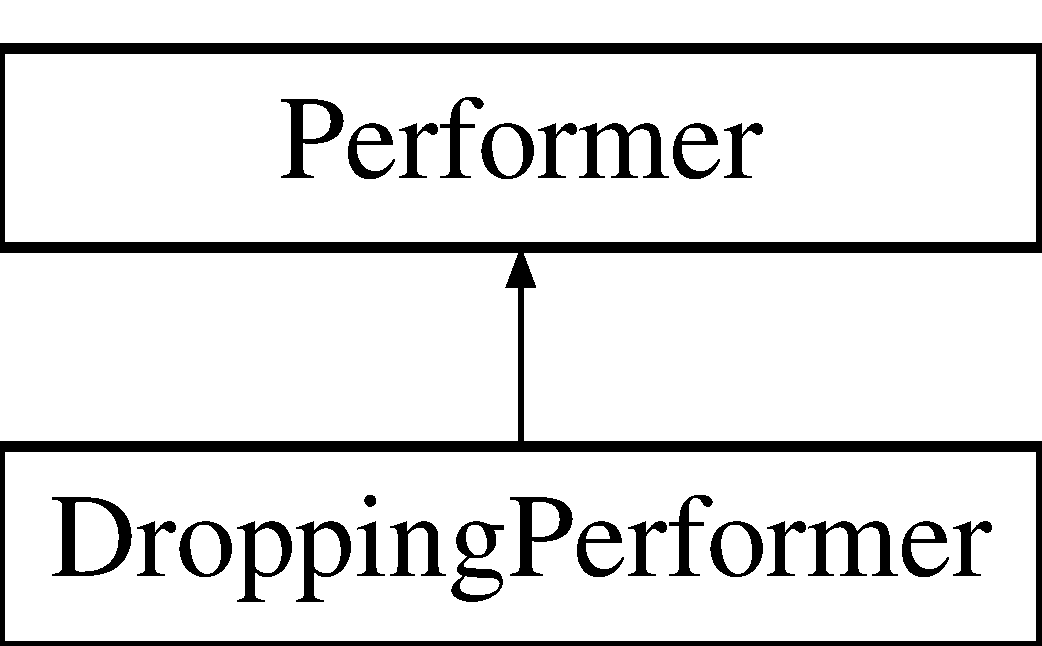
\includegraphics[height=2.000000cm]{classDroppingPerformer}
\end{center}
\end{figure}
\subsection*{Public Member Functions}
\begin{DoxyCompactItemize}
\item 
\hyperlink{classDroppingPerformer_a5a507b3572ae68a347b67bd4e1e96cd9}{Dropping\-Performer} (\hyperlink{classWorld}{World} $\ast$world)
\begin{DoxyCompactList}\small\item\em Constructor for a particular world. \end{DoxyCompactList}\item 
\hyperlink{classDroppingPerformer_abdec9c06463e6f5a4b43fda65b52afd4}{$\sim$\-Dropping\-Performer} ()
\begin{DoxyCompactList}\small\item\em Destructor. \end{DoxyCompactList}\item 
void \hyperlink{classDroppingPerformer_a1e3c90d034e5e6a7333484668e3c5cc4}{perform} (\hyperlink{classAction}{Action} \&action)
\begin{DoxyCompactList}\small\item\em Check if an object can move and move it. \end{DoxyCompactList}\end{DoxyCompactItemize}


\subsection{Detailed Description}
Performs a drop if possible. 

Definition at line 16 of file Dropping\-Performer.\-h.



\subsection{Constructor \& Destructor Documentation}
\hypertarget{classDroppingPerformer_a5a507b3572ae68a347b67bd4e1e96cd9}{\index{Dropping\-Performer@{Dropping\-Performer}!Dropping\-Performer@{Dropping\-Performer}}
\index{Dropping\-Performer@{Dropping\-Performer}!DroppingPerformer@{Dropping\-Performer}}
\subsubsection[{Dropping\-Performer}]{\setlength{\rightskip}{0pt plus 5cm}Dropping\-Performer\-::\-Dropping\-Performer (
\begin{DoxyParamCaption}
\item[{{\bf World} $\ast$}]{world}
\end{DoxyParamCaption}
)}}\label{classDroppingPerformer_a5a507b3572ae68a347b67bd4e1e96cd9}


Constructor for a particular world. 


\begin{DoxyParams}{Parameters}
{\em world\-\_\-size} & size of the world \\
\hline
{\em indexator} & indexator \\
\hline
\end{DoxyParams}


Definition at line 25 of file Dropping\-Performer.\-cpp.

\hypertarget{classDroppingPerformer_abdec9c06463e6f5a4b43fda65b52afd4}{\index{Dropping\-Performer@{Dropping\-Performer}!$\sim$\-Dropping\-Performer@{$\sim$\-Dropping\-Performer}}
\index{$\sim$\-Dropping\-Performer@{$\sim$\-Dropping\-Performer}!DroppingPerformer@{Dropping\-Performer}}
\subsubsection[{$\sim$\-Dropping\-Performer}]{\setlength{\rightskip}{0pt plus 5cm}Dropping\-Performer\-::$\sim$\-Dropping\-Performer (
\begin{DoxyParamCaption}
{}
\end{DoxyParamCaption}
)}}\label{classDroppingPerformer_abdec9c06463e6f5a4b43fda65b52afd4}


Destructor. 



Definition at line 30 of file Dropping\-Performer.\-cpp.



\subsection{Member Function Documentation}
\hypertarget{classDroppingPerformer_a1e3c90d034e5e6a7333484668e3c5cc4}{\index{Dropping\-Performer@{Dropping\-Performer}!perform@{perform}}
\index{perform@{perform}!DroppingPerformer@{Dropping\-Performer}}
\subsubsection[{perform}]{\setlength{\rightskip}{0pt plus 5cm}void Dropping\-Performer\-::perform (
\begin{DoxyParamCaption}
\item[{{\bf Action} \&}]{action}
\end{DoxyParamCaption}
)\hspace{0.3cm}{\ttfamily [virtual]}}}\label{classDroppingPerformer_a1e3c90d034e5e6a7333484668e3c5cc4}


Check if an object can move and move it. 


\begin{DoxyParams}{Parameters}
{\em action} & a request for moving \\
\hline
\end{DoxyParams}


Implements \hyperlink{classPerformer_a4cfa828ea1f9f07fd1aa9d330adfb5d5}{Performer}.



Definition at line 34 of file Dropping\-Performer.\-cpp.



The documentation for this class was generated from the following files\-:\begin{DoxyCompactItemize}
\item 
control/\-Performer/\-Dropping\-Performer/\hyperlink{DroppingPerformer_8h}{Dropping\-Performer.\-h}\item 
control/\-Performer/\-Dropping\-Performer/\hyperlink{DroppingPerformer_8cpp}{Dropping\-Performer.\-cpp}\end{DoxyCompactItemize}

\hypertarget{classEParamArrayBadKey}{\section{E\-Param\-Array\-Bad\-Key Class Reference}
\label{classEParamArrayBadKey}\index{E\-Param\-Array\-Bad\-Key@{E\-Param\-Array\-Bad\-Key}}
}


\hyperlink{classParamArray}{Param\-Array} exception -- unknown (bad) key was used.  




{\ttfamily \#include $<$E\-Param\-Array\-Bad\-Key.\-h$>$}



\subsection{Detailed Description}
\hyperlink{classParamArray}{Param\-Array} exception -- unknown (bad) key was used. 

Definition at line 9 of file E\-Param\-Array\-Bad\-Key.\-h.



The documentation for this class was generated from the following files\-:\begin{DoxyCompactItemize}
\item 
model/\-World/\-Param\-Array/\hyperlink{EParamArrayBadKey_8h}{E\-Param\-Array\-Bad\-Key.\-h}\item 
model/\-World/\-Param\-Array/\hyperlink{EParamArrayBadKey_8cpp}{E\-Param\-Array\-Bad\-Key.\-cpp}\end{DoxyCompactItemize}

\hypertarget{classGod}{\section{God Class Reference}
\label{classGod}\index{God@{God}}
}


\hyperlink{classGod}{God} class.  




{\ttfamily \#include $<$God.\-h$>$}

\subsection*{Public Member Functions}
\begin{DoxyCompactItemize}
\item 
\hyperlink{classGod_addc6776ed9e06891a0a19f28e945e5c3}{God} ()
\begin{DoxyCompactList}\small\item\em Constructor. \end{DoxyCompactList}\item 
\hyperlink{classGod_a905bb10f55a27a73b5d1550ed7dd582d}{$\sim$\-God} ()
\begin{DoxyCompactList}\small\item\em Destructor. \end{DoxyCompactList}\end{DoxyCompactItemize}


\subsection{Detailed Description}
\hyperlink{classGod}{God} class. 

Definition at line 15 of file God.\-h.



\subsection{Constructor \& Destructor Documentation}
\hypertarget{classGod_addc6776ed9e06891a0a19f28e945e5c3}{\index{God@{God}!God@{God}}
\index{God@{God}!God@{God}}
\subsubsection[{God}]{\setlength{\rightskip}{0pt plus 5cm}God\-::\-God (
\begin{DoxyParamCaption}
{}
\end{DoxyParamCaption}
)}}\label{classGod_addc6776ed9e06891a0a19f28e945e5c3}


Constructor. 



Definition at line 12 of file God.\-cpp.

\hypertarget{classGod_a905bb10f55a27a73b5d1550ed7dd582d}{\index{God@{God}!$\sim$\-God@{$\sim$\-God}}
\index{$\sim$\-God@{$\sim$\-God}!God@{God}}
\subsubsection[{$\sim$\-God}]{\setlength{\rightskip}{0pt plus 5cm}God\-::$\sim$\-God (
\begin{DoxyParamCaption}
{}
\end{DoxyParamCaption}
)}}\label{classGod_a905bb10f55a27a73b5d1550ed7dd582d}


Destructor. 



Definition at line 17 of file God.\-cpp.



The documentation for this class was generated from the following files\-:\begin{DoxyCompactItemize}
\item 
model/\-God/\hyperlink{God_8h}{God.\-h}\item 
model/\-God/\hyperlink{God_8cpp}{God.\-cpp}\end{DoxyCompactItemize}

\hypertarget{classHarmPerformer}{\section{Harm\-Performer Class Reference}
\label{classHarmPerformer}\index{Harm\-Performer@{Harm\-Performer}}
}


Performs a harm if it is possible.  




{\ttfamily \#include $<$Harm\-Performer.\-h$>$}

Inheritance diagram for Harm\-Performer\-:\begin{figure}[H]
\begin{center}
\leavevmode
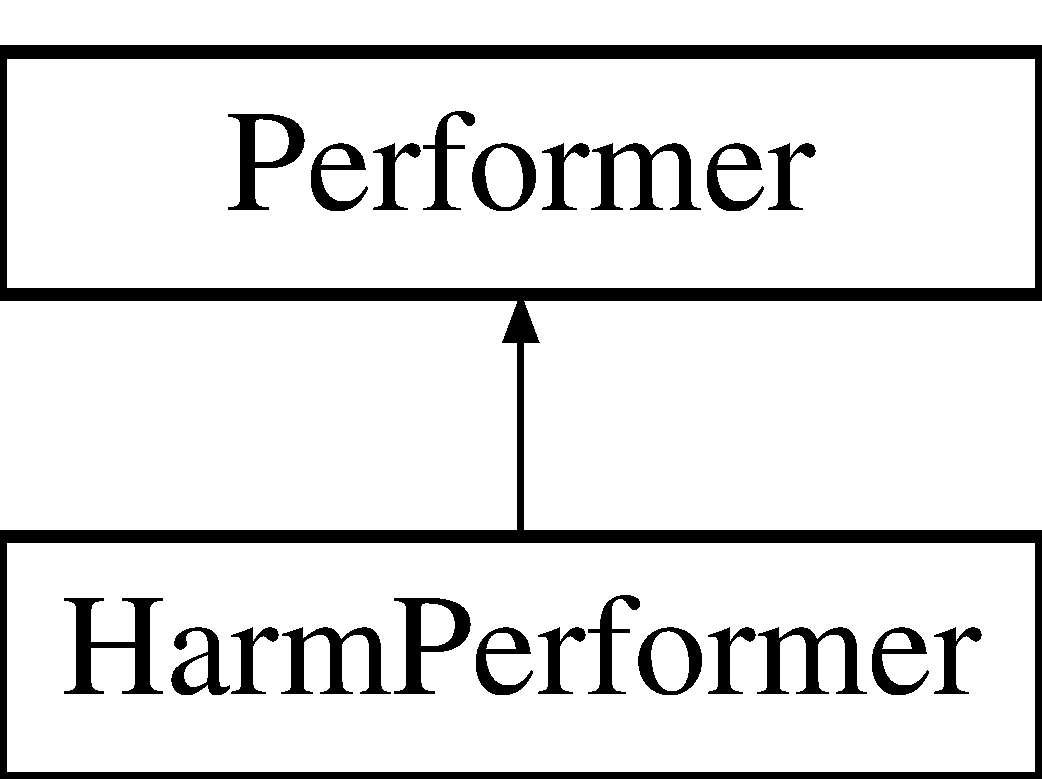
\includegraphics[height=2.000000cm]{classHarmPerformer}
\end{center}
\end{figure}
\subsection*{Public Member Functions}
\begin{DoxyCompactItemize}
\item 
\hyperlink{classHarmPerformer_a4df21e699f3cfc7501398221da29d11a}{Harm\-Performer} (\hyperlink{classIndexator}{Indexator} \&indexator)
\begin{DoxyCompactList}\small\item\em Constructor. \end{DoxyCompactList}\item 
\hyperlink{classHarmPerformer_a0c1d9f1e442a5926c2f8b1b7b294c9aa}{$\sim$\-Harm\-Performer} ()
\begin{DoxyCompactList}\small\item\em Destructor. \end{DoxyCompactList}\item 
void \hyperlink{classHarmPerformer_a58a611a6b7cd808b9e57fb6b5123701c}{perform} (\hyperlink{classAction}{Action} \&action)
\begin{DoxyCompactList}\small\item\em Check if an object can harm. \end{DoxyCompactList}\end{DoxyCompactItemize}


\subsection{Detailed Description}
Performs a harm if it is possible. 

Definition at line 16 of file Harm\-Performer.\-h.



\subsection{Constructor \& Destructor Documentation}
\hypertarget{classHarmPerformer_a4df21e699f3cfc7501398221da29d11a}{\index{Harm\-Performer@{Harm\-Performer}!Harm\-Performer@{Harm\-Performer}}
\index{Harm\-Performer@{Harm\-Performer}!HarmPerformer@{Harm\-Performer}}
\subsubsection[{Harm\-Performer}]{\setlength{\rightskip}{0pt plus 5cm}Harm\-Performer\-::\-Harm\-Performer (
\begin{DoxyParamCaption}
\item[{{\bf Indexator} \&}]{indexator}
\end{DoxyParamCaption}
)}}\label{classHarmPerformer_a4df21e699f3cfc7501398221da29d11a}


Constructor. 



Definition at line 14 of file Harm\-Performer.\-cpp.

\hypertarget{classHarmPerformer_a0c1d9f1e442a5926c2f8b1b7b294c9aa}{\index{Harm\-Performer@{Harm\-Performer}!$\sim$\-Harm\-Performer@{$\sim$\-Harm\-Performer}}
\index{$\sim$\-Harm\-Performer@{$\sim$\-Harm\-Performer}!HarmPerformer@{Harm\-Performer}}
\subsubsection[{$\sim$\-Harm\-Performer}]{\setlength{\rightskip}{0pt plus 5cm}Harm\-Performer\-::$\sim$\-Harm\-Performer (
\begin{DoxyParamCaption}
{}
\end{DoxyParamCaption}
)}}\label{classHarmPerformer_a0c1d9f1e442a5926c2f8b1b7b294c9aa}


Destructor. 



Definition at line 20 of file Harm\-Performer.\-cpp.



\subsection{Member Function Documentation}
\hypertarget{classHarmPerformer_a58a611a6b7cd808b9e57fb6b5123701c}{\index{Harm\-Performer@{Harm\-Performer}!perform@{perform}}
\index{perform@{perform}!HarmPerformer@{Harm\-Performer}}
\subsubsection[{perform}]{\setlength{\rightskip}{0pt plus 5cm}void Harm\-Performer\-::perform (
\begin{DoxyParamCaption}
\item[{{\bf Action} \&}]{action}
\end{DoxyParamCaption}
)\hspace{0.3cm}{\ttfamily [virtual]}}}\label{classHarmPerformer_a58a611a6b7cd808b9e57fb6b5123701c}


Check if an object can harm. 


\begin{DoxyParams}{Parameters}
{\em action} & a request for harm \\
\hline
\end{DoxyParams}


Implements \hyperlink{classPerformer_a4cfa828ea1f9f07fd1aa9d330adfb5d5}{Performer}.



Definition at line 25 of file Harm\-Performer.\-cpp.



The documentation for this class was generated from the following files\-:\begin{DoxyCompactItemize}
\item 
control/\-Performer/\-Harm\-Performer/\hyperlink{HarmPerformer_8h}{Harm\-Performer.\-h}\item 
control/\-Performer/\-Harm\-Performer/\hyperlink{HarmPerformer_8cpp}{Harm\-Performer.\-cpp}\end{DoxyCompactItemize}

\hypertarget{classHumanoid}{\section{Humanoid Class Reference}
\label{classHumanoid}\index{Humanoid@{Humanoid}}
}


\hyperlink{classHumanoid}{Humanoid} is clever creature, has own ideals, thoughts and preferences. Humanoids are base element in game, they makes their own decisions and influence and change world around them.  




{\ttfamily \#include $<$Humanoid.\-h$>$}

Inheritance diagram for Humanoid\-:\begin{figure}[H]
\begin{center}
\leavevmode
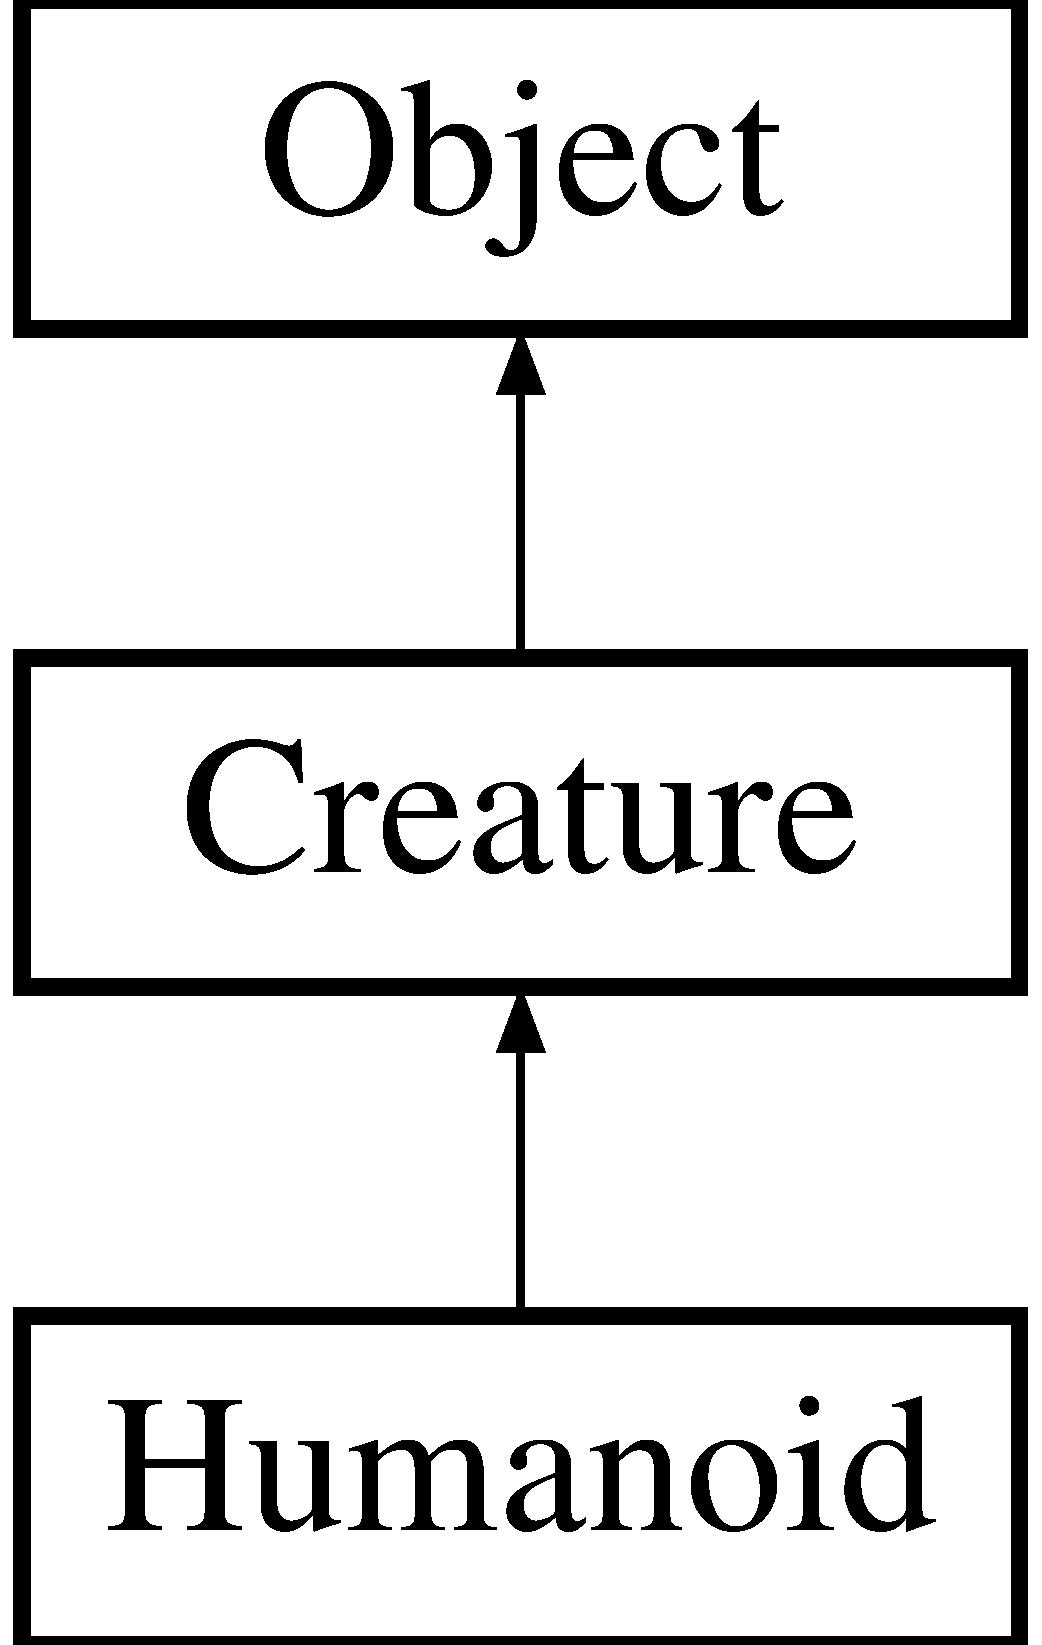
\includegraphics[height=3.000000cm]{classHumanoid}
\end{center}
\end{figure}
\subsection*{Public Member Functions}
\begin{DoxyCompactItemize}
\item 
\hyperlink{classHumanoid_af3565e2c74410d3c411bc94224e5de29}{Humanoid} (const \hyperlink{classDecisionMaker}{Decision\-Maker} \&dmaker)
\begin{DoxyCompactList}\small\item\em Random constructor (creates \hyperlink{classHumanoid}{Humanoid} with really random attributes). \end{DoxyCompactList}\item 
virtual \hyperlink{classHumanoid_a72dbc95208cb84fc3a70691f310e61ee}{$\sim$\-Humanoid} ()
\begin{DoxyCompactList}\small\item\em Destructor. \end{DoxyCompactList}\item 
std\-::vector$<$ \hyperlink{classAction}{Action} $>$ $\ast$ \hyperlink{classHumanoid_a543dfc658e59e98f5194aa64dd2ae723}{get\-Actions} ()
\begin{DoxyCompactList}\small\item\em Gets actions. \end{DoxyCompactList}\end{DoxyCompactItemize}
\subsection*{Additional Inherited Members}


\subsection{Detailed Description}
\hyperlink{classHumanoid}{Humanoid} is clever creature, has own ideals, thoughts and preferences. Humanoids are base element in game, they makes their own decisions and influence and change world around them. 

Definition at line 19 of file Humanoid.\-h.



\subsection{Constructor \& Destructor Documentation}
\hypertarget{classHumanoid_af3565e2c74410d3c411bc94224e5de29}{\index{Humanoid@{Humanoid}!Humanoid@{Humanoid}}
\index{Humanoid@{Humanoid}!Humanoid@{Humanoid}}
\subsubsection[{Humanoid}]{\setlength{\rightskip}{0pt plus 5cm}Humanoid\-::\-Humanoid (
\begin{DoxyParamCaption}
\item[{const {\bf Decision\-Maker} \&}]{dmaker}
\end{DoxyParamCaption}
)}}\label{classHumanoid_af3565e2c74410d3c411bc94224e5de29}


Random constructor (creates \hyperlink{classHumanoid}{Humanoid} with really random attributes). 


\begin{DoxyParams}{Parameters}
{\em dmaker} & humanoid's decision maker \\
\hline
\end{DoxyParams}


Definition at line 21 of file Humanoid.\-cpp.

\hypertarget{classHumanoid_a72dbc95208cb84fc3a70691f310e61ee}{\index{Humanoid@{Humanoid}!$\sim$\-Humanoid@{$\sim$\-Humanoid}}
\index{$\sim$\-Humanoid@{$\sim$\-Humanoid}!Humanoid@{Humanoid}}
\subsubsection[{$\sim$\-Humanoid}]{\setlength{\rightskip}{0pt plus 5cm}Humanoid\-::$\sim$\-Humanoid (
\begin{DoxyParamCaption}
{}
\end{DoxyParamCaption}
)\hspace{0.3cm}{\ttfamily [virtual]}}}\label{classHumanoid_a72dbc95208cb84fc3a70691f310e61ee}


Destructor. 



Definition at line 57 of file Humanoid.\-cpp.



\subsection{Member Function Documentation}
\hypertarget{classHumanoid_a543dfc658e59e98f5194aa64dd2ae723}{\index{Humanoid@{Humanoid}!get\-Actions@{get\-Actions}}
\index{get\-Actions@{get\-Actions}!Humanoid@{Humanoid}}
\subsubsection[{get\-Actions}]{\setlength{\rightskip}{0pt plus 5cm}std\-::vector$<$ {\bf Action} $>$ $\ast$ Humanoid\-::get\-Actions (
\begin{DoxyParamCaption}
{}
\end{DoxyParamCaption}
)\hspace{0.3cm}{\ttfamily [virtual]}}}\label{classHumanoid_a543dfc658e59e98f5194aa64dd2ae723}


Gets actions. 

\begin{DoxyReturn}{Returns}
vector with actions. 
\end{DoxyReturn}


Implements \hyperlink{classObject_addf0658ee2f8da579d10a6682dc097d7}{Object}.



Definition at line 62 of file Humanoid.\-cpp.



The documentation for this class was generated from the following files\-:\begin{DoxyCompactItemize}
\item 
model/\-World/\-Object/\-Creatures/\-Humanoid/\hyperlink{Humanoid_8h}{Humanoid.\-h}\item 
model/\-World/\-Object/\-Creatures/\-Humanoid/\hyperlink{Humanoid_8cpp}{Humanoid.\-cpp}\end{DoxyCompactItemize}

\hypertarget{classIndexator}{\section{Indexator Class Reference}
\label{classIndexator}\index{Indexator@{Indexator}}
}


{\ttfamily \#include $<$Indexator.\-h$>$}

\subsection*{Public Member Functions}
\begin{DoxyCompactItemize}
\item 
\hyperlink{classIndexator_aa5adafc65a3b10399adb6f2158bc5417}{Indexator} (double size, \hyperlink{classObjectHeap}{Object\-Heap} $\ast$list=0)
\begin{DoxyCompactList}\small\item\em Creates grid and indexates object from heap. \end{DoxyCompactList}\item 
\hyperlink{classIndexator_a1d84445c20808fddf2f8877cfd968a5b}{$\sim$\-Indexator} ()
\begin{DoxyCompactList}\small\item\em Destructor. \end{DoxyCompactList}\item 
\hyperlink{classObjectHeap}{Object\-Heap} $\ast$ \hyperlink{classIndexator_a21eb2f0f155c5d3fe0560a707a05e450}{get\-Area\-Contents} (\hyperlink{classShape}{Shape} area)
\begin{DoxyCompactList}\small\item\em Returns heap with objects from the certain area. \end{DoxyCompactList}\item 
void \hyperlink{classIndexator_ad3ee911b9f5cd04c2c6426dd90bce127}{reindexate} (\hyperlink{classObjectHeap}{Object\-Heap} $\ast$objects)
\begin{DoxyCompactList}\small\item\em Creates an index for all given objects, and removes the previous one. \end{DoxyCompactList}\item 
void \hyperlink{classIndexator_a3c496109b375bc095e15a38d2e8f18d8}{reindexate} (\hyperlink{classObject}{Object} $\ast$object)
\begin{DoxyCompactList}\small\item\em Reindexates an object or adds new object to index. \end{DoxyCompactList}\item 
void \hyperlink{classIndexator_aebbad325d23422a61443742e2d315f2c}{add\-Object} (\hyperlink{classObject}{Object} $\ast$object)
\begin{DoxyCompactList}\small\item\em Adds object to index. \end{DoxyCompactList}\item 
void \hyperlink{classIndexator_a494d579d9b7444788099ee9f57ba6420}{remove\-Object} (\hyperlink{classObject}{Object} $\ast$object)
\begin{DoxyCompactList}\small\item\em Removes object from index. \end{DoxyCompactList}\end{DoxyCompactItemize}


\subsection{Detailed Description}


Definition at line 24 of file Indexator.\-h.



\subsection{Constructor \& Destructor Documentation}
\hypertarget{classIndexator_aa5adafc65a3b10399adb6f2158bc5417}{\index{Indexator@{Indexator}!Indexator@{Indexator}}
\index{Indexator@{Indexator}!Indexator@{Indexator}}
\subsubsection[{Indexator}]{\setlength{\rightskip}{0pt plus 5cm}Indexator\-::\-Indexator (
\begin{DoxyParamCaption}
\item[{double}]{size, }
\item[{{\bf Object\-Heap} $\ast$}]{list = {\ttfamily 0}}
\end{DoxyParamCaption}
)}}\label{classIndexator_aa5adafc65a3b10399adb6f2158bc5417}


Creates grid and indexates object from heap. 


\begin{DoxyParams}{Parameters}
{\em list} & heap with objects \\
\hline
{\em size} & size of the world \\
\hline
\end{DoxyParams}


Definition at line 14 of file Indexator.\-cpp.

\hypertarget{classIndexator_a1d84445c20808fddf2f8877cfd968a5b}{\index{Indexator@{Indexator}!$\sim$\-Indexator@{$\sim$\-Indexator}}
\index{$\sim$\-Indexator@{$\sim$\-Indexator}!Indexator@{Indexator}}
\subsubsection[{$\sim$\-Indexator}]{\setlength{\rightskip}{0pt plus 5cm}Indexator\-::$\sim$\-Indexator (
\begin{DoxyParamCaption}
{}
\end{DoxyParamCaption}
)}}\label{classIndexator_a1d84445c20808fddf2f8877cfd968a5b}


Destructor. 



Definition at line 33 of file Indexator.\-cpp.



\subsection{Member Function Documentation}
\hypertarget{classIndexator_aebbad325d23422a61443742e2d315f2c}{\index{Indexator@{Indexator}!add\-Object@{add\-Object}}
\index{add\-Object@{add\-Object}!Indexator@{Indexator}}
\subsubsection[{add\-Object}]{\setlength{\rightskip}{0pt plus 5cm}void Indexator\-::add\-Object (
\begin{DoxyParamCaption}
\item[{{\bf Object} $\ast$}]{object}
\end{DoxyParamCaption}
)}}\label{classIndexator_aebbad325d23422a61443742e2d315f2c}


Adds object to index. 


\begin{DoxyParams}{Parameters}
{\em object} & an object to add \\
\hline
\end{DoxyParams}


Definition at line 218 of file Indexator.\-cpp.

\hypertarget{classIndexator_a21eb2f0f155c5d3fe0560a707a05e450}{\index{Indexator@{Indexator}!get\-Area\-Contents@{get\-Area\-Contents}}
\index{get\-Area\-Contents@{get\-Area\-Contents}!Indexator@{Indexator}}
\subsubsection[{get\-Area\-Contents}]{\setlength{\rightskip}{0pt plus 5cm}{\bf Object\-Heap} $\ast$ Indexator\-::get\-Area\-Contents (
\begin{DoxyParamCaption}
\item[{{\bf Shape}}]{area}
\end{DoxyParamCaption}
)}}\label{classIndexator_a21eb2f0f155c5d3fe0560a707a05e450}


Returns heap with objects from the certain area. 


\begin{DoxyParams}{Parameters}
{\em area} & where to look for objects \\
\hline
\end{DoxyParams}
\begin{DoxyReturn}{Returns}
heap with objects in given area 
\end{DoxyReturn}
\begin{DoxyVerb}    Toroidal feature
\end{DoxyVerb}
 Create more areas to check collisions with objects intersecting bounds of the world \hyperlink{classShape}{Shape} areas\mbox{[}4\mbox{]}; areas\mbox{[}0\mbox{]} = area; \hyperlink{classPoint}{Point} center = area.\-get\-Center();

Get the left bottom shape if (center.\-get\-X() $>$ world\-\_\-size/2) \{ if (center.\-get\-Y() $>$ world\-\_\-size / 2) \{ areas\mbox{[}0\mbox{]}.set\-Center(center -\/ Point(world\-\_\-size, world\-\_\-size)); \} else \{ areas\mbox{[}0\mbox{]}.set\-Center(center -\/ Point(world\-\_\-size, 0)); \} \} else \{ if (center.\-get\-Y() $>$ world\-\_\-size / 2) \{ areas\mbox{[}0\mbox{]}.set\-Center(center -\/ Point(0, world\-\_\-size)); \} \}

Creat all other shapes areas\mbox{[}1\mbox{]} = areas\mbox{[}0\mbox{]}; areas\mbox{[}1\mbox{]}.set\-Center(areas\mbox{[}0\mbox{]}.get\-Center() + Point(0, world\-\_\-size)); areas\mbox{[}2\mbox{]} = areas\mbox{[}1\mbox{]}; areas\mbox{[}2\mbox{]}.set\-Center(areas\mbox{[}1\mbox{]}.get\-Center() + Point(world\-\_\-size, 0)); areas\mbox{[}3\mbox{]} = areas\mbox{[}2\mbox{]}; areas\mbox{[}3\mbox{]}.set\-Center(areas\mbox{[}2\mbox{]}.get\-Center() + \hyperlink{classPoint}{Point}(0, -\/world\-\_\-size));

Definition at line 43 of file Indexator.\-cpp.

\hypertarget{classIndexator_ad3ee911b9f5cd04c2c6426dd90bce127}{\index{Indexator@{Indexator}!reindexate@{reindexate}}
\index{reindexate@{reindexate}!Indexator@{Indexator}}
\subsubsection[{reindexate}]{\setlength{\rightskip}{0pt plus 5cm}void Indexator\-::reindexate (
\begin{DoxyParamCaption}
\item[{{\bf Object\-Heap} $\ast$}]{objects}
\end{DoxyParamCaption}
)}}\label{classIndexator_ad3ee911b9f5cd04c2c6426dd90bce127}


Creates an index for all given objects, and removes the previous one. 


\begin{DoxyParams}{Parameters}
{\em objects} & heap of objects \\
\hline
\end{DoxyParams}


Definition at line 127 of file Indexator.\-cpp.

\hypertarget{classIndexator_a3c496109b375bc095e15a38d2e8f18d8}{\index{Indexator@{Indexator}!reindexate@{reindexate}}
\index{reindexate@{reindexate}!Indexator@{Indexator}}
\subsubsection[{reindexate}]{\setlength{\rightskip}{0pt plus 5cm}void Indexator\-::reindexate (
\begin{DoxyParamCaption}
\item[{{\bf Object} $\ast$}]{object}
\end{DoxyParamCaption}
)}}\label{classIndexator_a3c496109b375bc095e15a38d2e8f18d8}


Reindexates an object or adds new object to index. 


\begin{DoxyParams}{Parameters}
{\em object} & an object t reindexate \\
\hline
\end{DoxyParams}


Definition at line 148 of file Indexator.\-cpp.

\hypertarget{classIndexator_a494d579d9b7444788099ee9f57ba6420}{\index{Indexator@{Indexator}!remove\-Object@{remove\-Object}}
\index{remove\-Object@{remove\-Object}!Indexator@{Indexator}}
\subsubsection[{remove\-Object}]{\setlength{\rightskip}{0pt plus 5cm}void Indexator\-::remove\-Object (
\begin{DoxyParamCaption}
\item[{{\bf Object} $\ast$}]{object}
\end{DoxyParamCaption}
)}}\label{classIndexator_a494d579d9b7444788099ee9f57ba6420}


Removes object from index. 


\begin{DoxyParams}{Parameters}
{\em object} & an object to remove \\
\hline
\end{DoxyParams}


Definition at line 236 of file Indexator.\-cpp.



The documentation for this class was generated from the following files\-:\begin{DoxyCompactItemize}
\item 
model/\-World/\-Indexator/\hyperlink{Indexator_8h}{Indexator.\-h}\item 
model/\-World/\-Indexator/\hyperlink{Indexator_8cpp}{Indexator.\-cpp}\end{DoxyCompactItemize}

\hypertarget{classIWorld}{\section{I\-World Class Reference}
\label{classIWorld}\index{I\-World@{I\-World}}
}


{\ttfamily \#include $<$I\-World.\-h$>$}

Inheritance diagram for I\-World\-:\begin{figure}[H]
\begin{center}
\leavevmode
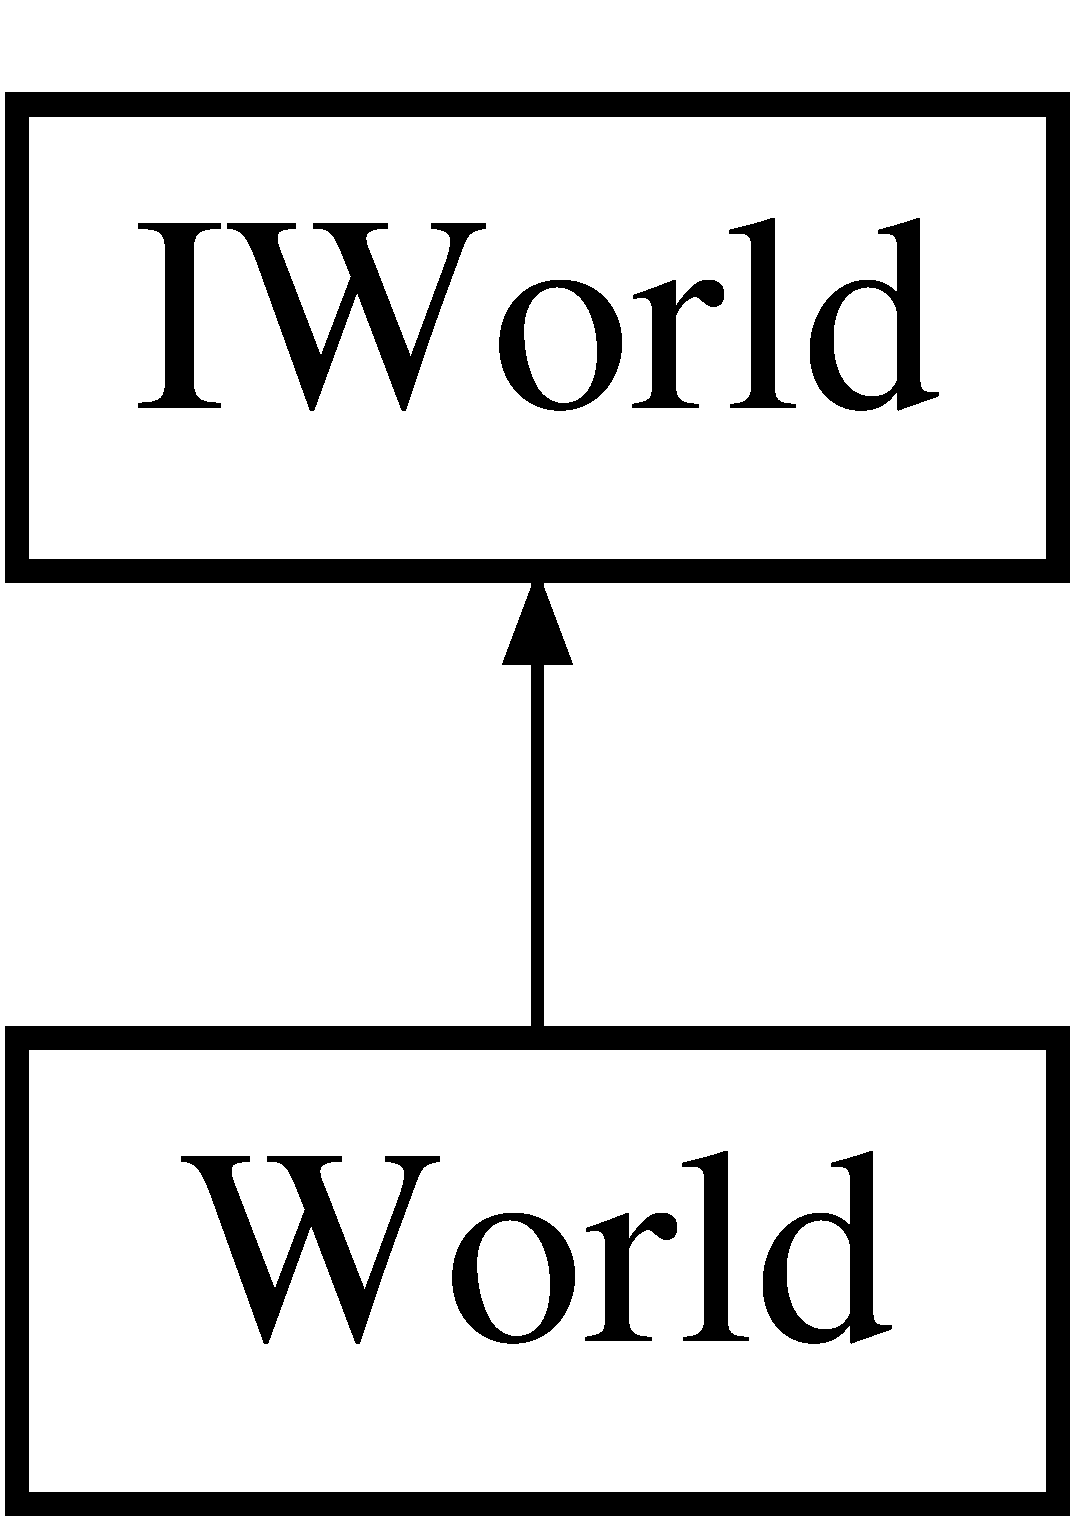
\includegraphics[height=2.000000cm]{classIWorld}
\end{center}
\end{figure}
\subsection*{Public Member Functions}
\begin{DoxyCompactItemize}
\item 
virtual \hyperlink{classIWorld_ab9a7fe6708d136457f27be89629143ed}{$\sim$\-I\-World} ()
\item 
virtual \hyperlink{classObjectHeap}{Object\-Heap} $\ast$ \hyperlink{classIWorld_aae71f283d70ad9f267d6731683e6ab7e}{get\-Visible\-Objects} ()=0
\item 
virtual \hyperlink{classObjectHeap}{Object\-Heap} $\ast$ \hyperlink{classIWorld_a1adf8090134ff1742c99b0dacd46b276}{get\-Hidden\-Objects} ()=0
\item 
virtual \hyperlink{classIndexator}{Indexator} $\ast$ \hyperlink{classIWorld_a75233893bfd7288b9e7306e08eb2a39d}{get\-Indexator} ()=0
\item 
virtual \hyperlink{classObjectFactory}{Object\-Factory} $\ast$ \hyperlink{classIWorld_a8deb54efc20b8b1d4b966fe5128c9c2b}{get\-Object\-Factory} ()=0
\item 
virtual double \hyperlink{classIWorld_a3791b170cd91f6d1a71ef958f19d2ac9}{get\-Size} ()=0
\item 
virtual \hyperlink{classObject}{Object} $\ast$$\ast$ \hyperlink{classIWorld_a7c94c8a5db44f1ae707f35e7c4fd3aef}{get\-View\-Objects\-In\-Range} (double x, double y, double radius)=0
\item 
virtual \hyperlink{BasicTypes_8h_aae2a79ad426e847c0ddfd77d04ce2516}{Weather\-Type} \hyperlink{classIWorld_ac3c29f9aba4066efbe3bbfce51030ad5}{get\-Weather\-At\-Point} (double x, double y)=0
\end{DoxyCompactItemize}


\subsection{Detailed Description}


Definition at line 13 of file I\-World.\-h.



\subsection{Constructor \& Destructor Documentation}
\hypertarget{classIWorld_ab9a7fe6708d136457f27be89629143ed}{\index{I\-World@{I\-World}!$\sim$\-I\-World@{$\sim$\-I\-World}}
\index{$\sim$\-I\-World@{$\sim$\-I\-World}!IWorld@{I\-World}}
\subsubsection[{$\sim$\-I\-World}]{\setlength{\rightskip}{0pt plus 5cm}virtual I\-World\-::$\sim$\-I\-World (
\begin{DoxyParamCaption}
{}
\end{DoxyParamCaption}
)\hspace{0.3cm}{\ttfamily [inline]}, {\ttfamily [virtual]}}}\label{classIWorld_ab9a7fe6708d136457f27be89629143ed}


Definition at line 16 of file I\-World.\-h.



\subsection{Member Function Documentation}
\hypertarget{classIWorld_a1adf8090134ff1742c99b0dacd46b276}{\index{I\-World@{I\-World}!get\-Hidden\-Objects@{get\-Hidden\-Objects}}
\index{get\-Hidden\-Objects@{get\-Hidden\-Objects}!IWorld@{I\-World}}
\subsubsection[{get\-Hidden\-Objects}]{\setlength{\rightskip}{0pt plus 5cm}virtual {\bf Object\-Heap}$\ast$ I\-World\-::get\-Hidden\-Objects (
\begin{DoxyParamCaption}
{}
\end{DoxyParamCaption}
)\hspace{0.3cm}{\ttfamily [pure virtual]}}}\label{classIWorld_a1adf8090134ff1742c99b0dacd46b276}


Implemented in \hyperlink{classWorld_acdde856cd58e64641405806d08650004}{World}.

\hypertarget{classIWorld_a75233893bfd7288b9e7306e08eb2a39d}{\index{I\-World@{I\-World}!get\-Indexator@{get\-Indexator}}
\index{get\-Indexator@{get\-Indexator}!IWorld@{I\-World}}
\subsubsection[{get\-Indexator}]{\setlength{\rightskip}{0pt plus 5cm}virtual {\bf Indexator}$\ast$ I\-World\-::get\-Indexator (
\begin{DoxyParamCaption}
{}
\end{DoxyParamCaption}
)\hspace{0.3cm}{\ttfamily [pure virtual]}}}\label{classIWorld_a75233893bfd7288b9e7306e08eb2a39d}


Implemented in \hyperlink{classWorld_ad75ce919ba59eb32d7b9aa4b1ec89ea6}{World}.

\hypertarget{classIWorld_a8deb54efc20b8b1d4b966fe5128c9c2b}{\index{I\-World@{I\-World}!get\-Object\-Factory@{get\-Object\-Factory}}
\index{get\-Object\-Factory@{get\-Object\-Factory}!IWorld@{I\-World}}
\subsubsection[{get\-Object\-Factory}]{\setlength{\rightskip}{0pt plus 5cm}virtual {\bf Object\-Factory}$\ast$ I\-World\-::get\-Object\-Factory (
\begin{DoxyParamCaption}
{}
\end{DoxyParamCaption}
)\hspace{0.3cm}{\ttfamily [pure virtual]}}}\label{classIWorld_a8deb54efc20b8b1d4b966fe5128c9c2b}


Implemented in \hyperlink{classWorld_a25dfb5e9ccd3dd5540ccf6f56937ec28}{World}.

\hypertarget{classIWorld_a3791b170cd91f6d1a71ef958f19d2ac9}{\index{I\-World@{I\-World}!get\-Size@{get\-Size}}
\index{get\-Size@{get\-Size}!IWorld@{I\-World}}
\subsubsection[{get\-Size}]{\setlength{\rightskip}{0pt plus 5cm}virtual double I\-World\-::get\-Size (
\begin{DoxyParamCaption}
{}
\end{DoxyParamCaption}
)\hspace{0.3cm}{\ttfamily [pure virtual]}}}\label{classIWorld_a3791b170cd91f6d1a71ef958f19d2ac9}


Implemented in \hyperlink{classWorld_a1c3e886903df2a4fcb8bff59e0dbf115}{World}.

\hypertarget{classIWorld_a7c94c8a5db44f1ae707f35e7c4fd3aef}{\index{I\-World@{I\-World}!get\-View\-Objects\-In\-Range@{get\-View\-Objects\-In\-Range}}
\index{get\-View\-Objects\-In\-Range@{get\-View\-Objects\-In\-Range}!IWorld@{I\-World}}
\subsubsection[{get\-View\-Objects\-In\-Range}]{\setlength{\rightskip}{0pt plus 5cm}virtual {\bf Object}$\ast$$\ast$ I\-World\-::get\-View\-Objects\-In\-Range (
\begin{DoxyParamCaption}
\item[{double}]{x, }
\item[{double}]{y, }
\item[{double}]{radius}
\end{DoxyParamCaption}
)\hspace{0.3cm}{\ttfamily [pure virtual]}}}\label{classIWorld_a7c94c8a5db44f1ae707f35e7c4fd3aef}


Implemented in \hyperlink{classWorld_a4e16dbeed23237902f74b62f229d7d20}{World}.

\hypertarget{classIWorld_aae71f283d70ad9f267d6731683e6ab7e}{\index{I\-World@{I\-World}!get\-Visible\-Objects@{get\-Visible\-Objects}}
\index{get\-Visible\-Objects@{get\-Visible\-Objects}!IWorld@{I\-World}}
\subsubsection[{get\-Visible\-Objects}]{\setlength{\rightskip}{0pt plus 5cm}virtual {\bf Object\-Heap}$\ast$ I\-World\-::get\-Visible\-Objects (
\begin{DoxyParamCaption}
{}
\end{DoxyParamCaption}
)\hspace{0.3cm}{\ttfamily [pure virtual]}}}\label{classIWorld_aae71f283d70ad9f267d6731683e6ab7e}


Implemented in \hyperlink{classWorld_ae7d9c8d7590bfa0ed18ed42c05106664}{World}.

\hypertarget{classIWorld_ac3c29f9aba4066efbe3bbfce51030ad5}{\index{I\-World@{I\-World}!get\-Weather\-At\-Point@{get\-Weather\-At\-Point}}
\index{get\-Weather\-At\-Point@{get\-Weather\-At\-Point}!IWorld@{I\-World}}
\subsubsection[{get\-Weather\-At\-Point}]{\setlength{\rightskip}{0pt plus 5cm}virtual {\bf Weather\-Type} I\-World\-::get\-Weather\-At\-Point (
\begin{DoxyParamCaption}
\item[{double}]{x, }
\item[{double}]{y}
\end{DoxyParamCaption}
)\hspace{0.3cm}{\ttfamily [pure virtual]}}}\label{classIWorld_ac3c29f9aba4066efbe3bbfce51030ad5}


Implemented in \hyperlink{classWorld_ab2c8d9f05cfbda5430d6a5e8f7754b85}{World}.



The documentation for this class was generated from the following file\-:\begin{DoxyCompactItemize}
\item 
model/\-World/\hyperlink{IWorld_8h}{I\-World.\-h}\end{DoxyCompactItemize}

\hypertarget{classKeyHandler}{\section{Key\-Handler Class Reference}
\label{classKeyHandler}\index{Key\-Handler@{Key\-Handler}}
}


{\ttfamily \#include $<$Key\-Handler.\-h$>$}

\subsection*{Public Member Functions}
\begin{DoxyCompactItemize}
\item 
\hyperlink{classKeyHandler_a9f90e60def9a242e88629dc6d6641789}{Key\-Handler} ()
\begin{DoxyCompactList}\small\item\em Constructor. \end{DoxyCompactList}\item 
\hyperlink{classKeyHandler_abcd8e7571a7a90ba891efa72f8d1bd51}{$\sim$\-Key\-Handler} ()
\begin{DoxyCompactList}\small\item\em Destructor. \end{DoxyCompactList}\item 
int \hyperlink{classKeyHandler_a78e381b671e5c6eca4af7b8aa4e40674}{handle\-Keys} ()
\begin{DoxyCompactList}\small\item\em Returns some enum indicating what action should be performed by \hyperlink{classView}{View}. \end{DoxyCompactList}\end{DoxyCompactItemize}


\subsection{Detailed Description}


Definition at line 11 of file Key\-Handler.\-h.



\subsection{Constructor \& Destructor Documentation}
\hypertarget{classKeyHandler_a9f90e60def9a242e88629dc6d6641789}{\index{Key\-Handler@{Key\-Handler}!Key\-Handler@{Key\-Handler}}
\index{Key\-Handler@{Key\-Handler}!KeyHandler@{Key\-Handler}}
\subsubsection[{Key\-Handler}]{\setlength{\rightskip}{0pt plus 5cm}Key\-Handler\-::\-Key\-Handler (
\begin{DoxyParamCaption}
{}
\end{DoxyParamCaption}
)}}\label{classKeyHandler_a9f90e60def9a242e88629dc6d6641789}


Constructor. 



Definition at line 7 of file Key\-Handler.\-cpp.

\hypertarget{classKeyHandler_abcd8e7571a7a90ba891efa72f8d1bd51}{\index{Key\-Handler@{Key\-Handler}!$\sim$\-Key\-Handler@{$\sim$\-Key\-Handler}}
\index{$\sim$\-Key\-Handler@{$\sim$\-Key\-Handler}!KeyHandler@{Key\-Handler}}
\subsubsection[{$\sim$\-Key\-Handler}]{\setlength{\rightskip}{0pt plus 5cm}Key\-Handler\-::$\sim$\-Key\-Handler (
\begin{DoxyParamCaption}
{}
\end{DoxyParamCaption}
)}}\label{classKeyHandler_abcd8e7571a7a90ba891efa72f8d1bd51}


Destructor. 



Definition at line 12 of file Key\-Handler.\-cpp.



\subsection{Member Function Documentation}
\hypertarget{classKeyHandler_a78e381b671e5c6eca4af7b8aa4e40674}{\index{Key\-Handler@{Key\-Handler}!handle\-Keys@{handle\-Keys}}
\index{handle\-Keys@{handle\-Keys}!KeyHandler@{Key\-Handler}}
\subsubsection[{handle\-Keys}]{\setlength{\rightskip}{0pt plus 5cm}int Key\-Handler\-::handle\-Keys (
\begin{DoxyParamCaption}
{}
\end{DoxyParamCaption}
)}}\label{classKeyHandler_a78e381b671e5c6eca4af7b8aa4e40674}


Returns some enum indicating what action should be performed by \hyperlink{classView}{View}. 



Definition at line 17 of file Key\-Handler.\-cpp.



The documentation for this class was generated from the following files\-:\begin{DoxyCompactItemize}
\item 
view/\-Key\-Handler/\hyperlink{KeyHandler_8h}{Key\-Handler.\-h}\item 
view/\-Key\-Handler/\hyperlink{KeyHandler_8cpp}{Key\-Handler.\-cpp}\end{DoxyCompactItemize}

\hypertarget{classMiningPerformer}{\section{Mining\-Performer Class Reference}
\label{classMiningPerformer}\index{Mining\-Performer@{Mining\-Performer}}
}


Performs a mining if it is possible.  




{\ttfamily \#include $<$Mining\-Performer.\-h$>$}

Inheritance diagram for Mining\-Performer\-:\begin{figure}[H]
\begin{center}
\leavevmode
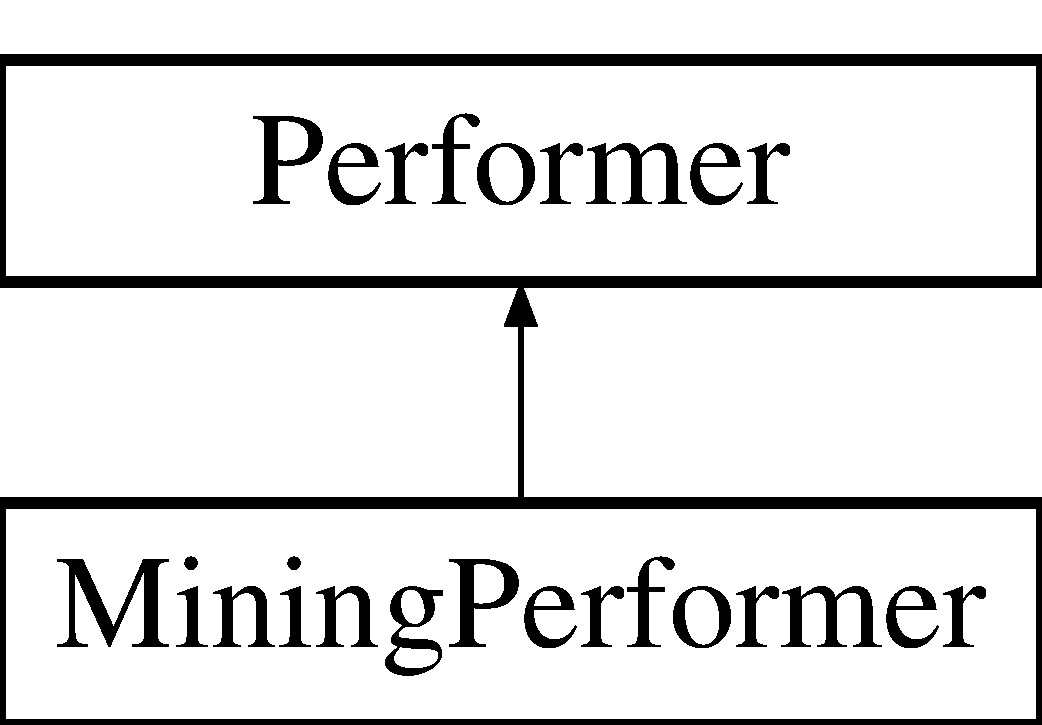
\includegraphics[height=2.000000cm]{classMiningPerformer}
\end{center}
\end{figure}
\subsection*{Public Member Functions}
\begin{DoxyCompactItemize}
\item 
\hyperlink{classMiningPerformer_a479529b5ff8ada471ad4185ac5b8fd5e}{Mining\-Performer} (\hyperlink{classIndexator}{Indexator} \&indexator)
\begin{DoxyCompactList}\small\item\em Constructor. \end{DoxyCompactList}\item 
\hyperlink{classMiningPerformer_a9855d33e82be8f645d9c54b47f5fdad7}{$\sim$\-Mining\-Performer} ()
\begin{DoxyCompactList}\small\item\em Destructor. \end{DoxyCompactList}\item 
void \hyperlink{classMiningPerformer_abfc1f91322ab3dd52af98a4cb6e3f30b}{perform} (\hyperlink{classAction}{Action} \&action)
\begin{DoxyCompactList}\small\item\em Check if an object can mine and mine it. \end{DoxyCompactList}\end{DoxyCompactItemize}


\subsection{Detailed Description}
Performs a mining if it is possible. 

Definition at line 19 of file Mining\-Performer.\-h.



\subsection{Constructor \& Destructor Documentation}
\hypertarget{classMiningPerformer_a479529b5ff8ada471ad4185ac5b8fd5e}{\index{Mining\-Performer@{Mining\-Performer}!Mining\-Performer@{Mining\-Performer}}
\index{Mining\-Performer@{Mining\-Performer}!MiningPerformer@{Mining\-Performer}}
\subsubsection[{Mining\-Performer}]{\setlength{\rightskip}{0pt plus 5cm}Mining\-Performer\-::\-Mining\-Performer (
\begin{DoxyParamCaption}
\item[{{\bf Indexator} \&}]{indexator}
\end{DoxyParamCaption}
)}}\label{classMiningPerformer_a479529b5ff8ada471ad4185ac5b8fd5e}


Constructor. 



Definition at line 9 of file Mining\-Performer.\-cpp.

\hypertarget{classMiningPerformer_a9855d33e82be8f645d9c54b47f5fdad7}{\index{Mining\-Performer@{Mining\-Performer}!$\sim$\-Mining\-Performer@{$\sim$\-Mining\-Performer}}
\index{$\sim$\-Mining\-Performer@{$\sim$\-Mining\-Performer}!MiningPerformer@{Mining\-Performer}}
\subsubsection[{$\sim$\-Mining\-Performer}]{\setlength{\rightskip}{0pt plus 5cm}Mining\-Performer\-::$\sim$\-Mining\-Performer (
\begin{DoxyParamCaption}
{}
\end{DoxyParamCaption}
)}}\label{classMiningPerformer_a9855d33e82be8f645d9c54b47f5fdad7}


Destructor. 



Definition at line 15 of file Mining\-Performer.\-cpp.



\subsection{Member Function Documentation}
\hypertarget{classMiningPerformer_abfc1f91322ab3dd52af98a4cb6e3f30b}{\index{Mining\-Performer@{Mining\-Performer}!perform@{perform}}
\index{perform@{perform}!MiningPerformer@{Mining\-Performer}}
\subsubsection[{perform}]{\setlength{\rightskip}{0pt plus 5cm}void Mining\-Performer\-::perform (
\begin{DoxyParamCaption}
\item[{{\bf Action} \&}]{action}
\end{DoxyParamCaption}
)\hspace{0.3cm}{\ttfamily [virtual]}}}\label{classMiningPerformer_abfc1f91322ab3dd52af98a4cb6e3f30b}


Check if an object can mine and mine it. 


\begin{DoxyParams}{Parameters}
{\em action} & a request for mining \\
\hline
\end{DoxyParams}


Implements \hyperlink{classPerformer_a4cfa828ea1f9f07fd1aa9d330adfb5d5}{Performer}.



Definition at line 19 of file Mining\-Performer.\-cpp.



The documentation for this class was generated from the following files\-:\begin{DoxyCompactItemize}
\item 
control/\-Performer/\-Mining\-Performer/\hyperlink{MiningPerformer_8h}{Mining\-Performer.\-h}\item 
control/\-Performer/\-Mining\-Performer/\hyperlink{MiningPerformer_8cpp}{Mining\-Performer.\-cpp}\end{DoxyCompactItemize}

\hypertarget{classMovementPerformer}{\section{Movement\-Performer Class Reference}
\label{classMovementPerformer}\index{Movement\-Performer@{Movement\-Performer}}
}


Performs a move if it is possible.  




{\ttfamily \#include $<$Movement\-Performer.\-h$>$}

Inheritance diagram for Movement\-Performer\-:\begin{figure}[H]
\begin{center}
\leavevmode
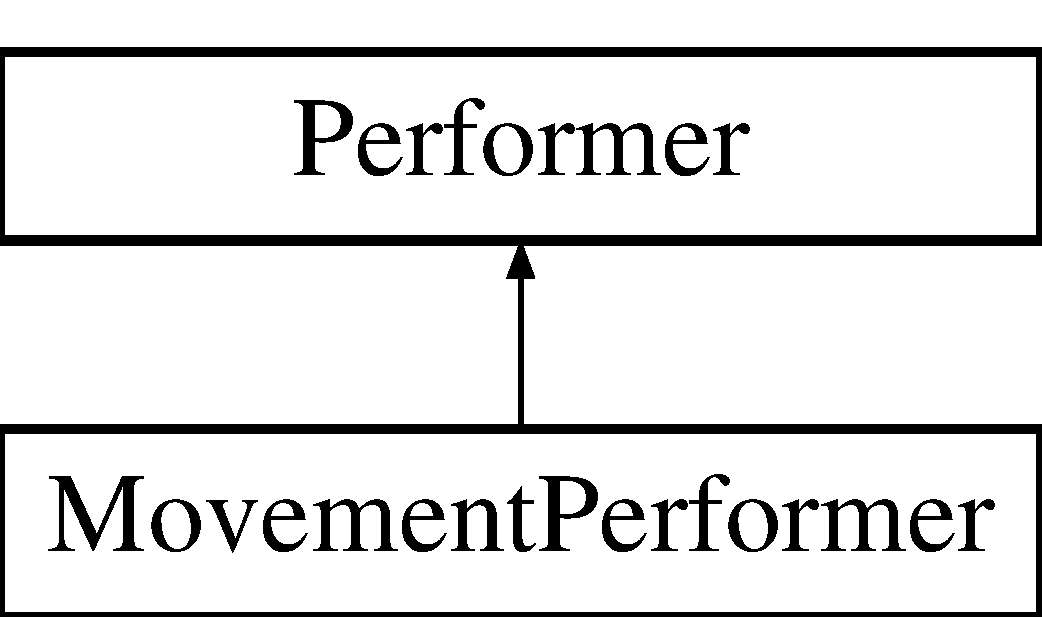
\includegraphics[height=2.000000cm]{classMovementPerformer}
\end{center}
\end{figure}
\subsection*{Public Member Functions}
\begin{DoxyCompactItemize}
\item 
\hyperlink{classMovementPerformer_a0d6336185e76b26141cfe7d2cd1d2066}{Movement\-Performer} (const double world\-\_\-size, \hyperlink{classIndexator}{Indexator} $\ast$indexator)
\begin{DoxyCompactList}\small\item\em Constructor for a particular world. \end{DoxyCompactList}\item 
\hyperlink{classMovementPerformer_a1715f190dbee77f4cc4a2c9a58a9064a}{$\sim$\-Movement\-Performer} ()
\begin{DoxyCompactList}\small\item\em Destructor. \end{DoxyCompactList}\item 
void \hyperlink{classMovementPerformer_aba62f523d2a9450a75fff98e350345b3}{perform} (\hyperlink{classAction}{Action} \&action)
\begin{DoxyCompactList}\small\item\em Check if an object can move and move it. \end{DoxyCompactList}\end{DoxyCompactItemize}


\subsection{Detailed Description}
Performs a move if it is possible. 

Definition at line 16 of file Movement\-Performer.\-h.



\subsection{Constructor \& Destructor Documentation}
\hypertarget{classMovementPerformer_a0d6336185e76b26141cfe7d2cd1d2066}{\index{Movement\-Performer@{Movement\-Performer}!Movement\-Performer@{Movement\-Performer}}
\index{Movement\-Performer@{Movement\-Performer}!MovementPerformer@{Movement\-Performer}}
\subsubsection[{Movement\-Performer}]{\setlength{\rightskip}{0pt plus 5cm}Movement\-Performer\-::\-Movement\-Performer (
\begin{DoxyParamCaption}
\item[{const double}]{world\-\_\-size, }
\item[{{\bf Indexator} $\ast$}]{indexator}
\end{DoxyParamCaption}
)}}\label{classMovementPerformer_a0d6336185e76b26141cfe7d2cd1d2066}


Constructor for a particular world. 


\begin{DoxyParams}{Parameters}
{\em world\-\_\-size} & size of the world \\
\hline
{\em indexator} & indexator \\
\hline
\end{DoxyParams}


Definition at line 24 of file Movement\-Performer.\-cpp.

\hypertarget{classMovementPerformer_a1715f190dbee77f4cc4a2c9a58a9064a}{\index{Movement\-Performer@{Movement\-Performer}!$\sim$\-Movement\-Performer@{$\sim$\-Movement\-Performer}}
\index{$\sim$\-Movement\-Performer@{$\sim$\-Movement\-Performer}!MovementPerformer@{Movement\-Performer}}
\subsubsection[{$\sim$\-Movement\-Performer}]{\setlength{\rightskip}{0pt plus 5cm}Movement\-Performer\-::$\sim$\-Movement\-Performer (
\begin{DoxyParamCaption}
{}
\end{DoxyParamCaption}
)}}\label{classMovementPerformer_a1715f190dbee77f4cc4a2c9a58a9064a}


Destructor. 



Definition at line 30 of file Movement\-Performer.\-cpp.



\subsection{Member Function Documentation}
\hypertarget{classMovementPerformer_aba62f523d2a9450a75fff98e350345b3}{\index{Movement\-Performer@{Movement\-Performer}!perform@{perform}}
\index{perform@{perform}!MovementPerformer@{Movement\-Performer}}
\subsubsection[{perform}]{\setlength{\rightskip}{0pt plus 5cm}void Movement\-Performer\-::perform (
\begin{DoxyParamCaption}
\item[{{\bf Action} \&}]{action}
\end{DoxyParamCaption}
)\hspace{0.3cm}{\ttfamily [virtual]}}}\label{classMovementPerformer_aba62f523d2a9450a75fff98e350345b3}


Check if an object can move and move it. 


\begin{DoxyParams}{Parameters}
{\em action} & a request for moving \\
\hline
\end{DoxyParams}


Implements \hyperlink{classPerformer_a4cfa828ea1f9f07fd1aa9d330adfb5d5}{Performer}.



Definition at line 34 of file Movement\-Performer.\-cpp.



The documentation for this class was generated from the following files\-:\begin{DoxyCompactItemize}
\item 
control/\-Performer/\-Movement\-Performer/\hyperlink{MovementPerformer_8h}{Movement\-Performer.\-h}\item 
control/\-Performer/\-Movement\-Performer/\hyperlink{MovementPerformer_8cpp}{Movement\-Performer.\-cpp}\end{DoxyCompactItemize}

\hypertarget{classNonHumanoid}{\section{Non\-Humanoid Class Reference}
\label{classNonHumanoid}\index{Non\-Humanoid@{Non\-Humanoid}}
}


\hyperlink{classNonHumanoid}{Non\-Humanoid} is silly creature, has only few goals in its life\-: food and sleep.  




{\ttfamily \#include $<$Non\-Humanoid.\-h$>$}

Inheritance diagram for Non\-Humanoid\-:\begin{figure}[H]
\begin{center}
\leavevmode
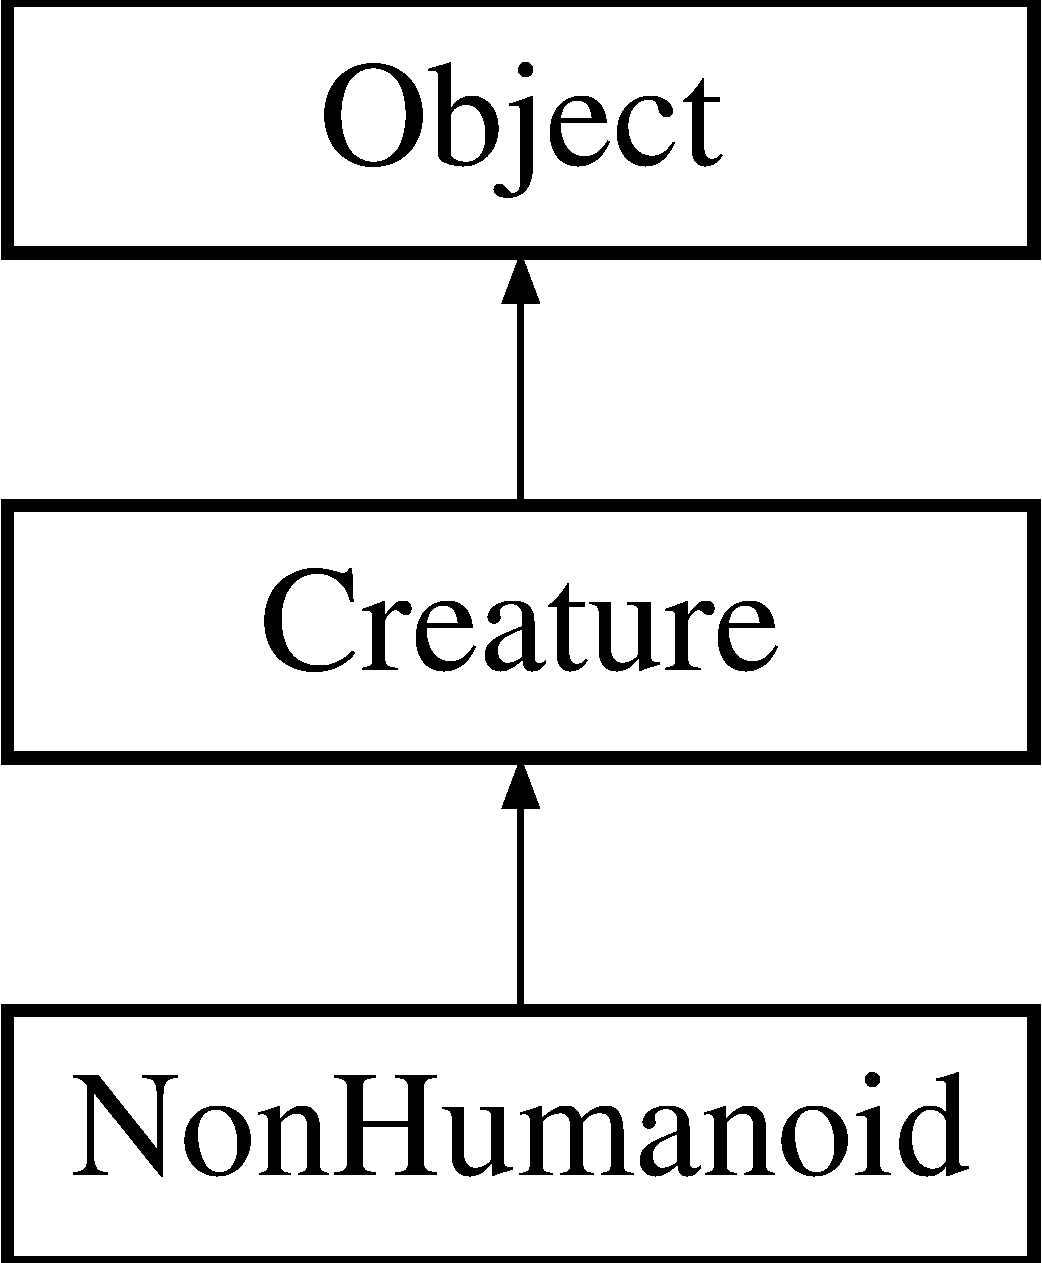
\includegraphics[height=3.000000cm]{classNonHumanoid}
\end{center}
\end{figure}
\subsection*{Public Member Functions}
\begin{DoxyCompactItemize}
\item 
\hyperlink{classNonHumanoid_aa8442222bc4b7e137bc939ba75a99c73}{Non\-Humanoid} (const \hyperlink{classDecisionMaker}{Decision\-Maker} \&dmaker)
\begin{DoxyCompactList}\small\item\em Random constructor (creates \hyperlink{classNonHumanoid}{Non\-Humanoid} with really random attributes). \end{DoxyCompactList}\item 
virtual \hyperlink{classNonHumanoid_a48709f30b26043f168fa5ebef55014e1}{$\sim$\-Non\-Humanoid} ()
\begin{DoxyCompactList}\small\item\em Destructor. \end{DoxyCompactList}\item 
std\-::vector$<$ \hyperlink{classAction}{Action} $>$ $\ast$ \hyperlink{classNonHumanoid_abc2fe4b8aeaa0a4bf2732fbdcbaf69bc}{get\-Actions} ()
\begin{DoxyCompactList}\small\item\em Gets actions. \end{DoxyCompactList}\end{DoxyCompactItemize}
\subsection*{Additional Inherited Members}


\subsection{Detailed Description}
\hyperlink{classNonHumanoid}{Non\-Humanoid} is silly creature, has only few goals in its life\-: food and sleep. 

Definition at line 16 of file Non\-Humanoid.\-h.



\subsection{Constructor \& Destructor Documentation}
\hypertarget{classNonHumanoid_aa8442222bc4b7e137bc939ba75a99c73}{\index{Non\-Humanoid@{Non\-Humanoid}!Non\-Humanoid@{Non\-Humanoid}}
\index{Non\-Humanoid@{Non\-Humanoid}!NonHumanoid@{Non\-Humanoid}}
\subsubsection[{Non\-Humanoid}]{\setlength{\rightskip}{0pt plus 5cm}Non\-Humanoid\-::\-Non\-Humanoid (
\begin{DoxyParamCaption}
\item[{const {\bf Decision\-Maker} \&}]{dmaker}
\end{DoxyParamCaption}
)}}\label{classNonHumanoid_aa8442222bc4b7e137bc939ba75a99c73}


Random constructor (creates \hyperlink{classNonHumanoid}{Non\-Humanoid} with really random attributes). 


\begin{DoxyParams}{Parameters}
{\em dmaker} & non-\/humanoid's decision maker \\
\hline
\end{DoxyParams}


Definition at line 19 of file Non\-Humanoid.\-cpp.

\hypertarget{classNonHumanoid_a48709f30b26043f168fa5ebef55014e1}{\index{Non\-Humanoid@{Non\-Humanoid}!$\sim$\-Non\-Humanoid@{$\sim$\-Non\-Humanoid}}
\index{$\sim$\-Non\-Humanoid@{$\sim$\-Non\-Humanoid}!NonHumanoid@{Non\-Humanoid}}
\subsubsection[{$\sim$\-Non\-Humanoid}]{\setlength{\rightskip}{0pt plus 5cm}Non\-Humanoid\-::$\sim$\-Non\-Humanoid (
\begin{DoxyParamCaption}
{}
\end{DoxyParamCaption}
)\hspace{0.3cm}{\ttfamily [virtual]}}}\label{classNonHumanoid_a48709f30b26043f168fa5ebef55014e1}


Destructor. 



Definition at line 59 of file Non\-Humanoid.\-cpp.



\subsection{Member Function Documentation}
\hypertarget{classNonHumanoid_abc2fe4b8aeaa0a4bf2732fbdcbaf69bc}{\index{Non\-Humanoid@{Non\-Humanoid}!get\-Actions@{get\-Actions}}
\index{get\-Actions@{get\-Actions}!NonHumanoid@{Non\-Humanoid}}
\subsubsection[{get\-Actions}]{\setlength{\rightskip}{0pt plus 5cm}std\-::vector$<$ {\bf Action} $>$ $\ast$ Non\-Humanoid\-::get\-Actions (
\begin{DoxyParamCaption}
{}
\end{DoxyParamCaption}
)\hspace{0.3cm}{\ttfamily [virtual]}}}\label{classNonHumanoid_abc2fe4b8aeaa0a4bf2732fbdcbaf69bc}


Gets actions. 

\begin{DoxyReturn}{Returns}
vector with actions. 
\end{DoxyReturn}


Implements \hyperlink{classObject_addf0658ee2f8da579d10a6682dc097d7}{Object}.



Definition at line 64 of file Non\-Humanoid.\-cpp.



The documentation for this class was generated from the following files\-:\begin{DoxyCompactItemize}
\item 
model/\-World/\-Object/\-Creatures/\-Non\-Humanoid/\hyperlink{NonHumanoid_8h}{Non\-Humanoid.\-h}\item 
model/\-World/\-Object/\-Creatures/\-Non\-Humanoid/\hyperlink{NonHumanoid_8cpp}{Non\-Humanoid.\-cpp}\end{DoxyCompactItemize}

\hypertarget{classObject}{\section{Object Class Reference}
\label{classObject}\index{Object@{Object}}
}


Abstract \hyperlink{classObject}{Object} class.  




{\ttfamily \#include $<$Object.\-h$>$}

Inheritance diagram for Object\-:\begin{figure}[H]
\begin{center}
\leavevmode
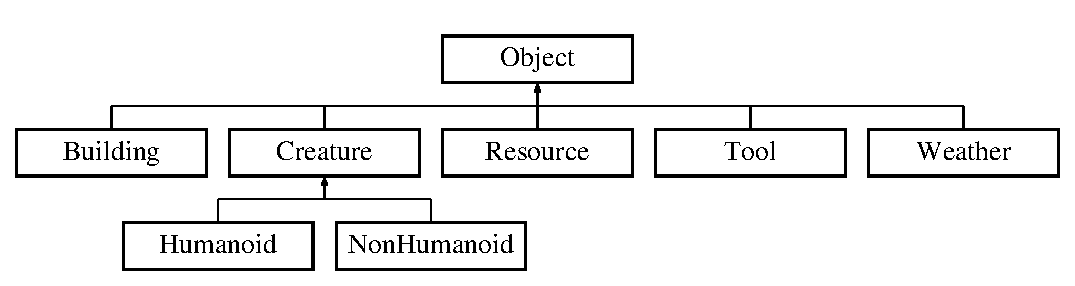
\includegraphics[height=3.000000cm]{classObject}
\end{center}
\end{figure}
\subsection*{Public Member Functions}
\begin{DoxyCompactItemize}
\item 
\hyperlink{classObject_a07e8b69a7746aa44c1e7784a08583729}{Object} (\hyperlink{BasicTypes_8h_a842c5e2e69277690b064bf363c017980}{Object\-Type} type)
\begin{DoxyCompactList}\small\item\em Constructor. \end{DoxyCompactList}\item 
virtual \hyperlink{classObject_ae8f5483f459e46687bd01e6f9977afd3}{$\sim$\-Object} ()
\begin{DoxyCompactList}\small\item\em Destructor. \end{DoxyCompactList}\item 
virtual std\-::vector$<$ \hyperlink{classAction}{Action} $>$ $\ast$ \hyperlink{classObject_addf0658ee2f8da579d10a6682dc097d7}{get\-Actions} ()=0
\begin{DoxyCompactList}\small\item\em Gets objects pending actions. \end{DoxyCompactList}\item 
virtual void \hyperlink{classObject_a816838bab5c67fce2cead6cb9122ad47}{damage} (\hyperlink{BasicTypes_8h_a91ad9478d81a7aaf2593e8d9c3d06a14}{uint} delta)=0
\begin{DoxyCompactList}\small\item\em Receives message. \end{DoxyCompactList}\item 
virtual void \hyperlink{classObject_af7f49cb3f3c3bd9cfdbc42beecbbe5bc}{heal} (\hyperlink{BasicTypes_8h_a91ad9478d81a7aaf2593e8d9c3d06a14}{uint} delta)=0
\begin{DoxyCompactList}\small\item\em Heals object. \end{DoxyCompactList}\item 
void \hyperlink{classObject_a9df0b8f5aef27057192b874ebd0d361e}{mark\-As\-Destroyed} ()
\begin{DoxyCompactList}\small\item\em Marks this object as destroyed. \end{DoxyCompactList}\item 
bool \hyperlink{classObject_a1e1a162b817f0c134836cca3a473e295}{is\-Destroyed} () const 
\begin{DoxyCompactList}\small\item\em Returns true if object is destroyed. \end{DoxyCompactList}\item 
void \hyperlink{classObject_ab810f6d0305506bb0803afcde852c1c8}{make\-Mortal} ()
\begin{DoxyCompactList}\small\item\em Makes object mortal. \end{DoxyCompactList}\item 
void \hyperlink{classObject_ad73c94472b9a43a629ae4cd6d2def67e}{make\-Immortal} ()
\begin{DoxyCompactList}\small\item\em Makes object immortal. \end{DoxyCompactList}\item 
bool \hyperlink{classObject_a7a38ff74620fa8c16a21e46149027e6a}{is\-Immortal} () const 
\begin{DoxyCompactList}\small\item\em Returns true if object is immortal. \end{DoxyCompactList}\item 
\hyperlink{BasicTypes_8h_a842c5e2e69277690b064bf363c017980}{Object\-Type} \hyperlink{classObject_a7660dc25529325326bc280e5f5fb0194}{get\-Type} () const 
\begin{DoxyCompactList}\small\item\em Get the value of type. \end{DoxyCompactList}\item 
void \hyperlink{classObject_a81450ac8abbba5ee97e2558cffabedf5}{set\-Shape\-Type} (\hyperlink{BasicTypes_8h_a5a4538eeab397888d88a4eefcc5a1345}{Shape\-Type} type)
\begin{DoxyCompactList}\small\item\em Sets object's shape type. \end{DoxyCompactList}\item 
void \hyperlink{classObject_af4a10aeb0de43db0d6bc43d6b6d9280b}{set\-Shape\-Size} (double size)
\begin{DoxyCompactList}\small\item\em Sets object's shape size. \end{DoxyCompactList}\item 
\hyperlink{classShape}{Shape} \hyperlink{classObject_ab55fd6193bbe9f7f4deb793222e79ca7}{get\-Shape} () const 
\begin{DoxyCompactList}\small\item\em Get the value of shape. \end{DoxyCompactList}\item 
void \hyperlink{classObject_a075891336e08ea144917d8468f8480f1}{set\-Angle} (double new\-\_\-var)
\begin{DoxyCompactList}\small\item\em Set the value of angle. \end{DoxyCompactList}\item 
double \hyperlink{classObject_aaba7ccef31e74246abda5ef9cb2e202c}{get\-Angle} () const 
\begin{DoxyCompactList}\small\item\em Get the value of angle. \end{DoxyCompactList}\item 
void \hyperlink{classObject_a67d41327686c2018494ea788379db9aa}{set\-Coords} (const \hyperlink{classPoint}{Point} \&coords)
\begin{DoxyCompactList}\small\item\em Set object's coordinates. \end{DoxyCompactList}\item 
const \hyperlink{classPoint}{Point} \& \hyperlink{classObject_a64bb5b1d10c6cd338a65a8dd62473de1}{get\-Coords} () const 
\begin{DoxyCompactList}\small\item\em Get object's coordinates. \end{DoxyCompactList}\end{DoxyCompactItemize}
\subsection*{Protected Attributes}
\begin{DoxyCompactItemize}
\item 
std\-::vector$<$ \hyperlink{classAction}{Action} $>$ \hyperlink{classObject_a7fa5bd0db11056aac9440fa9f6eb2690}{actions}
\begin{DoxyCompactList}\small\item\em Array with actions. \end{DoxyCompactList}\end{DoxyCompactItemize}


\subsection{Detailed Description}
Abstract \hyperlink{classObject}{Object} class. 

Definition at line 19 of file Object.\-h.



\subsection{Constructor \& Destructor Documentation}
\hypertarget{classObject_a07e8b69a7746aa44c1e7784a08583729}{\index{Object@{Object}!Object@{Object}}
\index{Object@{Object}!Object@{Object}}
\subsubsection[{Object}]{\setlength{\rightskip}{0pt plus 5cm}Object\-::\-Object (
\begin{DoxyParamCaption}
\item[{{\bf Object\-Type}}]{type}
\end{DoxyParamCaption}
)}}\label{classObject_a07e8b69a7746aa44c1e7784a08583729}


Constructor. 


\begin{DoxyParams}{Parameters}
{\em type} & Object\-Type \\
\hline
\end{DoxyParams}


Definition at line 14 of file Object.\-cpp.

\hypertarget{classObject_ae8f5483f459e46687bd01e6f9977afd3}{\index{Object@{Object}!$\sim$\-Object@{$\sim$\-Object}}
\index{$\sim$\-Object@{$\sim$\-Object}!Object@{Object}}
\subsubsection[{$\sim$\-Object}]{\setlength{\rightskip}{0pt plus 5cm}Object\-::$\sim$\-Object (
\begin{DoxyParamCaption}
{}
\end{DoxyParamCaption}
)\hspace{0.3cm}{\ttfamily [virtual]}}}\label{classObject_ae8f5483f459e46687bd01e6f9977afd3}


Destructor. 



Definition at line 24 of file Object.\-cpp.



\subsection{Member Function Documentation}
\hypertarget{classObject_a816838bab5c67fce2cead6cb9122ad47}{\index{Object@{Object}!damage@{damage}}
\index{damage@{damage}!Object@{Object}}
\subsubsection[{damage}]{\setlength{\rightskip}{0pt plus 5cm}virtual void Object\-::damage (
\begin{DoxyParamCaption}
\item[{{\bf uint}}]{delta}
\end{DoxyParamCaption}
)\hspace{0.3cm}{\ttfamily [pure virtual]}}}\label{classObject_a816838bab5c67fce2cead6cb9122ad47}


Receives message. 

Damages object. 
\begin{DoxyParams}{Parameters}
{\em delta} & amount of damage \\
\hline
\end{DoxyParams}


Implemented in \hyperlink{classCreature_a6d216fa9fc5e1a70743ebc9a62dbcc01}{Creature}, \hyperlink{classTool_aff5fb696dc98cf8892b4db6350495ca5}{Tool}, \hyperlink{classResource_aaba80262d4086bfce08ea4d4c0d63f75}{Resource}, \hyperlink{classBuilding_a6bb55b63a07e77ffea29316e8af400af}{Building}, and \hyperlink{classWeather_a2d2c127d06a55f388a80aedd07b6c2fb}{Weather}.

\hypertarget{classObject_addf0658ee2f8da579d10a6682dc097d7}{\index{Object@{Object}!get\-Actions@{get\-Actions}}
\index{get\-Actions@{get\-Actions}!Object@{Object}}
\subsubsection[{get\-Actions}]{\setlength{\rightskip}{0pt plus 5cm}virtual std\-::vector$<${\bf Action}$>$$\ast$ Object\-::get\-Actions (
\begin{DoxyParamCaption}
{}
\end{DoxyParamCaption}
)\hspace{0.3cm}{\ttfamily [pure virtual]}}}\label{classObject_addf0658ee2f8da579d10a6682dc097d7}


Gets objects pending actions. 

\begin{DoxyReturn}{Returns}
vector with pending actions. 
\end{DoxyReturn}


Implemented in \hyperlink{classResource_a4c4cc169461d76de8787c97276665168}{Resource}, \hyperlink{classHumanoid_a543dfc658e59e98f5194aa64dd2ae723}{Humanoid}, \hyperlink{classBuilding_a2b0b464d1d8aa158729b5e2f1454ecdf}{Building}, \hyperlink{classNonHumanoid_abc2fe4b8aeaa0a4bf2732fbdcbaf69bc}{Non\-Humanoid}, \hyperlink{classWeather_af6a985a031c55cc9d384fe532bbf69ef}{Weather}, and \hyperlink{classTool_a022fd16d7301835eff8324ef8447d90c}{Tool}.

\hypertarget{classObject_aaba7ccef31e74246abda5ef9cb2e202c}{\index{Object@{Object}!get\-Angle@{get\-Angle}}
\index{get\-Angle@{get\-Angle}!Object@{Object}}
\subsubsection[{get\-Angle}]{\setlength{\rightskip}{0pt plus 5cm}double Object\-::get\-Angle (
\begin{DoxyParamCaption}
{}
\end{DoxyParamCaption}
) const}}\label{classObject_aaba7ccef31e74246abda5ef9cb2e202c}


Get the value of angle. 

\begin{DoxyReturn}{Returns}
the value of angle 
\end{DoxyReturn}


Definition at line 95 of file Object.\-cpp.

\hypertarget{classObject_a64bb5b1d10c6cd338a65a8dd62473de1}{\index{Object@{Object}!get\-Coords@{get\-Coords}}
\index{get\-Coords@{get\-Coords}!Object@{Object}}
\subsubsection[{get\-Coords}]{\setlength{\rightskip}{0pt plus 5cm}const {\bf Point} \& Object\-::get\-Coords (
\begin{DoxyParamCaption}
{}
\end{DoxyParamCaption}
) const}}\label{classObject_a64bb5b1d10c6cd338a65a8dd62473de1}


Get object's coordinates. 

\begin{DoxyReturn}{Returns}
object's coordinates 
\end{DoxyReturn}


Definition at line 105 of file Object.\-cpp.

\hypertarget{classObject_ab55fd6193bbe9f7f4deb793222e79ca7}{\index{Object@{Object}!get\-Shape@{get\-Shape}}
\index{get\-Shape@{get\-Shape}!Object@{Object}}
\subsubsection[{get\-Shape}]{\setlength{\rightskip}{0pt plus 5cm}{\bf Shape} Object\-::get\-Shape (
\begin{DoxyParamCaption}
{}
\end{DoxyParamCaption}
) const}}\label{classObject_ab55fd6193bbe9f7f4deb793222e79ca7}


Get the value of shape. 

\begin{DoxyReturn}{Returns}
the value of shape 
\end{DoxyReturn}


Definition at line 85 of file Object.\-cpp.

\hypertarget{classObject_a7660dc25529325326bc280e5f5fb0194}{\index{Object@{Object}!get\-Type@{get\-Type}}
\index{get\-Type@{get\-Type}!Object@{Object}}
\subsubsection[{get\-Type}]{\setlength{\rightskip}{0pt plus 5cm}{\bf Object\-Type} Object\-::get\-Type (
\begin{DoxyParamCaption}
{}
\end{DoxyParamCaption}
) const}}\label{classObject_a7660dc25529325326bc280e5f5fb0194}


Get the value of type. 

\begin{DoxyReturn}{Returns}
the value of type 
\end{DoxyReturn}


Definition at line 66 of file Object.\-cpp.

\hypertarget{classObject_af7f49cb3f3c3bd9cfdbc42beecbbe5bc}{\index{Object@{Object}!heal@{heal}}
\index{heal@{heal}!Object@{Object}}
\subsubsection[{heal}]{\setlength{\rightskip}{0pt plus 5cm}virtual void Object\-::heal (
\begin{DoxyParamCaption}
\item[{{\bf uint}}]{delta}
\end{DoxyParamCaption}
)\hspace{0.3cm}{\ttfamily [pure virtual]}}}\label{classObject_af7f49cb3f3c3bd9cfdbc42beecbbe5bc}


Heals object. 


\begin{DoxyParams}{Parameters}
{\em delta} & amount of healing \\
\hline
\end{DoxyParams}


Implemented in \hyperlink{classCreature_ab168ec8b1230205eb0dda7edbef60469}{Creature}, \hyperlink{classTool_ac7103fa90707cbc29ceb31bc7f941571}{Tool}, \hyperlink{classResource_a88928f89a1a538768dade43b0493ec6c}{Resource}, \hyperlink{classBuilding_a4266475915167761e483886535382f90}{Building}, and \hyperlink{classWeather_abe32b96dd46b0ce43b3b663a7b1de56c}{Weather}.

\hypertarget{classObject_a1e1a162b817f0c134836cca3a473e295}{\index{Object@{Object}!is\-Destroyed@{is\-Destroyed}}
\index{is\-Destroyed@{is\-Destroyed}!Object@{Object}}
\subsubsection[{is\-Destroyed}]{\setlength{\rightskip}{0pt plus 5cm}bool Object\-::is\-Destroyed (
\begin{DoxyParamCaption}
{}
\end{DoxyParamCaption}
) const}}\label{classObject_a1e1a162b817f0c134836cca3a473e295}


Returns true if object is destroyed. 

\begin{DoxyReturn}{Returns}
is object destroyed or not 
\end{DoxyReturn}


Definition at line 38 of file Object.\-cpp.

\hypertarget{classObject_a7a38ff74620fa8c16a21e46149027e6a}{\index{Object@{Object}!is\-Immortal@{is\-Immortal}}
\index{is\-Immortal@{is\-Immortal}!Object@{Object}}
\subsubsection[{is\-Immortal}]{\setlength{\rightskip}{0pt plus 5cm}bool Object\-::is\-Immortal (
\begin{DoxyParamCaption}
{}
\end{DoxyParamCaption}
) const}}\label{classObject_a7a38ff74620fa8c16a21e46149027e6a}


Returns true if object is immortal. 

\begin{DoxyReturn}{Returns}
is object immortal or not 
\end{DoxyReturn}


Definition at line 57 of file Object.\-cpp.

\hypertarget{classObject_ad73c94472b9a43a629ae4cd6d2def67e}{\index{Object@{Object}!make\-Immortal@{make\-Immortal}}
\index{make\-Immortal@{make\-Immortal}!Object@{Object}}
\subsubsection[{make\-Immortal}]{\setlength{\rightskip}{0pt plus 5cm}void Object\-::make\-Immortal (
\begin{DoxyParamCaption}
{}
\end{DoxyParamCaption}
)}}\label{classObject_ad73c94472b9a43a629ae4cd6d2def67e}


Makes object immortal. 



Definition at line 52 of file Object.\-cpp.

\hypertarget{classObject_ab810f6d0305506bb0803afcde852c1c8}{\index{Object@{Object}!make\-Mortal@{make\-Mortal}}
\index{make\-Mortal@{make\-Mortal}!Object@{Object}}
\subsubsection[{make\-Mortal}]{\setlength{\rightskip}{0pt plus 5cm}void Object\-::make\-Mortal (
\begin{DoxyParamCaption}
{}
\end{DoxyParamCaption}
)}}\label{classObject_ab810f6d0305506bb0803afcde852c1c8}


Makes object mortal. 



Definition at line 47 of file Object.\-cpp.

\hypertarget{classObject_a9df0b8f5aef27057192b874ebd0d361e}{\index{Object@{Object}!mark\-As\-Destroyed@{mark\-As\-Destroyed}}
\index{mark\-As\-Destroyed@{mark\-As\-Destroyed}!Object@{Object}}
\subsubsection[{mark\-As\-Destroyed}]{\setlength{\rightskip}{0pt plus 5cm}void Object\-::mark\-As\-Destroyed (
\begin{DoxyParamCaption}
{}
\end{DoxyParamCaption}
)}}\label{classObject_a9df0b8f5aef27057192b874ebd0d361e}


Marks this object as destroyed. 



Definition at line 33 of file Object.\-cpp.

\hypertarget{classObject_a075891336e08ea144917d8468f8480f1}{\index{Object@{Object}!set\-Angle@{set\-Angle}}
\index{set\-Angle@{set\-Angle}!Object@{Object}}
\subsubsection[{set\-Angle}]{\setlength{\rightskip}{0pt plus 5cm}void Object\-::set\-Angle (
\begin{DoxyParamCaption}
\item[{double}]{new\-\_\-var}
\end{DoxyParamCaption}
)}}\label{classObject_a075891336e08ea144917d8468f8480f1}


Set the value of angle. 


\begin{DoxyParams}{Parameters}
{\em new\-\_\-var} & the new value of angle \\
\hline
\end{DoxyParams}


Definition at line 90 of file Object.\-cpp.

\hypertarget{classObject_a67d41327686c2018494ea788379db9aa}{\index{Object@{Object}!set\-Coords@{set\-Coords}}
\index{set\-Coords@{set\-Coords}!Object@{Object}}
\subsubsection[{set\-Coords}]{\setlength{\rightskip}{0pt plus 5cm}void Object\-::set\-Coords (
\begin{DoxyParamCaption}
\item[{const {\bf Point} \&}]{coords}
\end{DoxyParamCaption}
)}}\label{classObject_a67d41327686c2018494ea788379db9aa}


Set object's coordinates. 


\begin{DoxyParams}{Parameters}
{\em coords} & new coordinates \\
\hline
\end{DoxyParams}


Definition at line 100 of file Object.\-cpp.

\hypertarget{classObject_af4a10aeb0de43db0d6bc43d6b6d9280b}{\index{Object@{Object}!set\-Shape\-Size@{set\-Shape\-Size}}
\index{set\-Shape\-Size@{set\-Shape\-Size}!Object@{Object}}
\subsubsection[{set\-Shape\-Size}]{\setlength{\rightskip}{0pt plus 5cm}void Object\-::set\-Shape\-Size (
\begin{DoxyParamCaption}
\item[{double}]{size}
\end{DoxyParamCaption}
)}}\label{classObject_af4a10aeb0de43db0d6bc43d6b6d9280b}


Sets object's shape size. 


\begin{DoxyParams}{Parameters}
{\em size} & shape size \\
\hline
\end{DoxyParams}


Definition at line 80 of file Object.\-cpp.

\hypertarget{classObject_a81450ac8abbba5ee97e2558cffabedf5}{\index{Object@{Object}!set\-Shape\-Type@{set\-Shape\-Type}}
\index{set\-Shape\-Type@{set\-Shape\-Type}!Object@{Object}}
\subsubsection[{set\-Shape\-Type}]{\setlength{\rightskip}{0pt plus 5cm}void Object\-::set\-Shape\-Type (
\begin{DoxyParamCaption}
\item[{{\bf Shape\-Type}}]{type}
\end{DoxyParamCaption}
)}}\label{classObject_a81450ac8abbba5ee97e2558cffabedf5}


Sets object's shape type. 


\begin{DoxyParams}{Parameters}
{\em type} & shape type \\
\hline
\end{DoxyParams}


Definition at line 75 of file Object.\-cpp.



\subsection{Member Data Documentation}
\hypertarget{classObject_a7fa5bd0db11056aac9440fa9f6eb2690}{\index{Object@{Object}!actions@{actions}}
\index{actions@{actions}!Object@{Object}}
\subsubsection[{actions}]{\setlength{\rightskip}{0pt plus 5cm}std\-::vector$<${\bf Action}$>$ Object\-::actions\hspace{0.3cm}{\ttfamily [protected]}}}\label{classObject_a7fa5bd0db11056aac9440fa9f6eb2690}


Array with actions. 



Definition at line 174 of file Object.\-h.



The documentation for this class was generated from the following files\-:\begin{DoxyCompactItemize}
\item 
model/\-World/\-Object/\hyperlink{Object_8h}{Object.\-h}\item 
model/\-World/\-Object/\hyperlink{Object_8cpp}{Object.\-cpp}\end{DoxyCompactItemize}

\hypertarget{classObjectFactory}{\section{Object\-Factory Class Reference}
\label{classObjectFactory}\index{Object\-Factory@{Object\-Factory}}
}


\hyperlink{classObject}{Object} factory allows to creates any objects (you need to provide \hyperlink{classParamArray}{Param\-Array} with parameters to do this).  




{\ttfamily \#include $<$Object\-Factory.\-h$>$}

\subsection*{Public Member Functions}
\begin{DoxyCompactItemize}
\item 
\hyperlink{classObjectFactory_a3a732c533e17d2f62b753138d9da0eb4}{Object\-Factory} (const \hyperlink{classDecisionMaker}{Decision\-Maker} \&hum\-\_\-dmaker, const \hyperlink{classDecisionMaker}{Decision\-Maker} \&nhum\-\_\-dmaker)
\begin{DoxyCompactList}\small\item\em Constructor. \end{DoxyCompactList}\item 
\hyperlink{classObjectFactory_a04a1138c18e740b8f0fd580b3d52af1c}{$\sim$\-Object\-Factory} ()
\begin{DoxyCompactList}\small\item\em Destructor. \end{DoxyCompactList}\item 
\hyperlink{classObject}{Object} $\ast$ \hyperlink{classObjectFactory_a6c7102f01ee8e5bf6a3ca562e2b2aba0}{create\-Object} (\hyperlink{BasicTypes_8h_a842c5e2e69277690b064bf363c017980}{Object\-Type} type, const \hyperlink{classParamArray}{Param\-Array} \&params)
\begin{DoxyCompactList}\small\item\em Creates new object. \end{DoxyCompactList}\end{DoxyCompactItemize}


\subsection{Detailed Description}
\hyperlink{classObject}{Object} factory allows to creates any objects (you need to provide \hyperlink{classParamArray}{Param\-Array} with parameters to do this). 

To create object with type T first of all you need to provide parameter {\ttfamily obj\-\_\-type}. Value of this param is Object\-Type (converted to int). For each object type a few parameters more are needed.

{\bfseries \hyperlink{classCreature}{Creature}}
\begin{DoxyItemize}
\item {\itshape creat\-\_\-type} -- Creature\-Type.
\end{DoxyItemize}

{\bfseries \hyperlink{classBuilding}{Building}}
\begin{DoxyItemize}
\item {\itshape max\-\_\-health} -- \hyperlink{classBuilding}{Building} health (uint).
\item {\itshape max\-\_\-space} -- \hyperlink{classBuilding}{Building} space (uint).
\end{DoxyItemize}

{\bfseries \hyperlink{classResource}{Resource}}
\begin{DoxyItemize}
\item {\itshape res\-\_\-type} -- Resource\-Type.
\item {\itshape res\-\_\-amount} -- amount of resource (uint) ($\ast$).
\end{DoxyItemize}

{\bfseries \hyperlink{classTool}{Tool}}
\begin{DoxyItemize}
\item {\itshape tool\-\_\-type} -- Tool\-Type.
\item {\itshape mat\-\_\-type} -- Resource\-Type of material.
\item {\itshape tool\-\_\-str} -- \hyperlink{classTool}{Tool}'s strength (uint) ($\ast$).
\end{DoxyItemize}

{\bfseries \hyperlink{classWeather}{Weather}}
\begin{DoxyItemize}
\item {\itshape weat\-\_\-type} -- Weather\-Type.
\item {\itshape weat\-\_\-steps} -- amount of steps that \hyperlink{classWeather}{Weather} will live (uint) ($\ast$).
\end{DoxyItemize}

{\bfseries Note}\-: $\ast$ -- leave 0 to pick random value. 

Definition at line 48 of file Object\-Factory.\-h.



\subsection{Constructor \& Destructor Documentation}
\hypertarget{classObjectFactory_a3a732c533e17d2f62b753138d9da0eb4}{\index{Object\-Factory@{Object\-Factory}!Object\-Factory@{Object\-Factory}}
\index{Object\-Factory@{Object\-Factory}!ObjectFactory@{Object\-Factory}}
\subsubsection[{Object\-Factory}]{\setlength{\rightskip}{0pt plus 5cm}Object\-Factory\-::\-Object\-Factory (
\begin{DoxyParamCaption}
\item[{const {\bf Decision\-Maker} \&}]{hum\-\_\-dmaker, }
\item[{const {\bf Decision\-Maker} \&}]{nhum\-\_\-dmaker}
\end{DoxyParamCaption}
)}}\label{classObjectFactory_a3a732c533e17d2f62b753138d9da0eb4}


Constructor. 



Definition at line 22 of file Object\-Factory.\-cpp.

\hypertarget{classObjectFactory_a04a1138c18e740b8f0fd580b3d52af1c}{\index{Object\-Factory@{Object\-Factory}!$\sim$\-Object\-Factory@{$\sim$\-Object\-Factory}}
\index{$\sim$\-Object\-Factory@{$\sim$\-Object\-Factory}!ObjectFactory@{Object\-Factory}}
\subsubsection[{$\sim$\-Object\-Factory}]{\setlength{\rightskip}{0pt plus 5cm}Object\-Factory\-::$\sim$\-Object\-Factory (
\begin{DoxyParamCaption}
{}
\end{DoxyParamCaption}
)}}\label{classObjectFactory_a04a1138c18e740b8f0fd580b3d52af1c}


Destructor. 



Definition at line 29 of file Object\-Factory.\-cpp.



\subsection{Member Function Documentation}
\hypertarget{classObjectFactory_a6c7102f01ee8e5bf6a3ca562e2b2aba0}{\index{Object\-Factory@{Object\-Factory}!create\-Object@{create\-Object}}
\index{create\-Object@{create\-Object}!ObjectFactory@{Object\-Factory}}
\subsubsection[{create\-Object}]{\setlength{\rightskip}{0pt plus 5cm}{\bf Object} $\ast$ Object\-Factory\-::create\-Object (
\begin{DoxyParamCaption}
\item[{{\bf Object\-Type}}]{type, }
\item[{const {\bf Param\-Array} \&}]{params}
\end{DoxyParamCaption}
)}}\label{classObjectFactory_a6c7102f01ee8e5bf6a3ca562e2b2aba0}


Creates new object. 


\begin{DoxyParams}{Parameters}
{\em type} & object type \\
\hline
{\em params} & map with object params \\
\hline
\end{DoxyParams}
\begin{DoxyReturn}{Returns}
pointer to created object 
\end{DoxyReturn}


Definition at line 37 of file Object\-Factory.\-cpp.



The documentation for this class was generated from the following files\-:\begin{DoxyCompactItemize}
\item 
model/\-World/\-Object\-Factory/\hyperlink{ObjectFactory_8h}{Object\-Factory.\-h}\item 
model/\-World/\-Object\-Factory/\hyperlink{ObjectFactory_8cpp}{Object\-Factory.\-cpp}\end{DoxyCompactItemize}

\hypertarget{classObjectHeap}{\section{Object\-Heap Class Reference}
\label{classObjectHeap}\index{Object\-Heap@{Object\-Heap}}
}


\hyperlink{classObjectHeap}{Object\-Heap} class.  




{\ttfamily \#include $<$Object\-Heap.\-h$>$}

\subsection*{Public Types}
\begin{DoxyCompactItemize}
\item 
typedef std\-::vector$<$ \hyperlink{classObject}{Object} $\ast$ $>$\\*
\-::\hyperlink{classObjectHeap_a5be9fee885fae47d7dc090899d9fb7bd}{iterator} \hyperlink{classObjectHeap_a5be9fee885fae47d7dc090899d9fb7bd}{iterator}
\item 
typedef std\-::vector$<$ \hyperlink{classObject}{Object} $\ast$ $>$\\*
\-::\hyperlink{classObjectHeap_af07744bc1ca895917429540266b2b9bd}{const\-\_\-iterator} \hyperlink{classObjectHeap_af07744bc1ca895917429540266b2b9bd}{const\-\_\-iterator}
\end{DoxyCompactItemize}
\subsection*{Public Member Functions}
\begin{DoxyCompactItemize}
\item 
\hyperlink{classObjectHeap_a04488dc0dacc31b8f7f08c20716d447b}{Object\-Heap} ()
\begin{DoxyCompactList}\small\item\em Constructor. \end{DoxyCompactList}\item 
\hyperlink{classObjectHeap_a601b8bace5f8e425c90cc018b083b751}{$\sim$\-Object\-Heap} ()
\begin{DoxyCompactList}\small\item\em Destructor. \end{DoxyCompactList}\item 
unsigned int \hyperlink{classObjectHeap_a5320eb7e37dd7bfa968935b61d9f00bd}{get\-Amount} ()
\begin{DoxyCompactList}\small\item\em get amount of element \end{DoxyCompactList}\item 
unsigned int \hyperlink{classObjectHeap_aa864246aff54535535bffa4a779f6d8a}{get\-Type\-Amount} (\hyperlink{BasicTypes_8h_a842c5e2e69277690b064bf363c017980}{Object\-Type})
\begin{DoxyCompactList}\small\item\em get amount of element this type \end{DoxyCompactList}\item 
bool \hyperlink{classObjectHeap_a31aed12bfcff1455f1682cdb816184a6}{push} (\hyperlink{classObject}{Object} $\ast$object)
\begin{DoxyCompactList}\small\item\em Pushes object to heap. \end{DoxyCompactList}\item 
bool \hyperlink{classObjectHeap_a7092926b107145c62f0a6c8bd8ff1028}{remove} (\hyperlink{classObject}{Object} $\ast$object)
\begin{DoxyCompactList}\small\item\em Removes object from heap. \end{DoxyCompactList}\item 
\hyperlink{classObjectHeap_a5be9fee885fae47d7dc090899d9fb7bd}{iterator} \hyperlink{classObjectHeap_a3fa3502f08c4016bbcfcf8578e245d15}{begin} (\hyperlink{BasicTypes_8h_a842c5e2e69277690b064bf363c017980}{Object\-Type} type)
\item 
\hyperlink{classObjectHeap_af07744bc1ca895917429540266b2b9bd}{const\-\_\-iterator} \hyperlink{classObjectHeap_ac0c481b7e2d2d1901f73073d453b9b35}{begin} (\hyperlink{BasicTypes_8h_a842c5e2e69277690b064bf363c017980}{Object\-Type} type) const 
\item 
\hyperlink{classObjectHeap_a5be9fee885fae47d7dc090899d9fb7bd}{iterator} \hyperlink{classObjectHeap_a6b530e67b5383a29be3699f891c7482b}{end} (\hyperlink{BasicTypes_8h_a842c5e2e69277690b064bf363c017980}{Object\-Type} type)
\item 
\hyperlink{classObjectHeap_af07744bc1ca895917429540266b2b9bd}{const\-\_\-iterator} \hyperlink{classObjectHeap_a9e0ace11a93deb7163989cf6e3f4e88f}{end} (\hyperlink{BasicTypes_8h_a842c5e2e69277690b064bf363c017980}{Object\-Type} type) const 
\item 
\hyperlink{classObjectHeap_a5be9fee885fae47d7dc090899d9fb7bd}{iterator} \hyperlink{classObjectHeap_ae7be29d4f5049397b3c2dff7bd27016b}{begin} ()
\item 
\hyperlink{classObjectHeap_af07744bc1ca895917429540266b2b9bd}{const\-\_\-iterator} \hyperlink{classObjectHeap_aa27cac54482c7bf5aab561eddbcaa97a}{begin} () const 
\item 
\hyperlink{classObjectHeap_a5be9fee885fae47d7dc090899d9fb7bd}{iterator} \hyperlink{classObjectHeap_ab225091de1b80c054a545bab2c11b0fe}{end} ()
\item 
\hyperlink{classObjectHeap_af07744bc1ca895917429540266b2b9bd}{const\-\_\-iterator} \hyperlink{classObjectHeap_a366c6aedfc59ff2f84b70e68e1a4d266}{end} () const 
\item 
\hyperlink{classObjectHeap_a5be9fee885fae47d7dc090899d9fb7bd}{iterator} \hyperlink{classObjectHeap_a78e16a9ebe6bfe6c10f356fdd5cb5704}{find} (\hyperlink{classObject}{Object} $\ast$obj, bool return\-\_\-obj\-\_\-type\-\_\-iter=true)
\end{DoxyCompactItemize}


\subsection{Detailed Description}
\hyperlink{classObjectHeap}{Object\-Heap} class. 

Definition at line 20 of file Object\-Heap.\-h.



\subsection{Member Typedef Documentation}
\hypertarget{classObjectHeap_af07744bc1ca895917429540266b2b9bd}{\index{Object\-Heap@{Object\-Heap}!const\-\_\-iterator@{const\-\_\-iterator}}
\index{const\-\_\-iterator@{const\-\_\-iterator}!ObjectHeap@{Object\-Heap}}
\subsubsection[{const\-\_\-iterator}]{\setlength{\rightskip}{0pt plus 5cm}typedef std\-::vector$<${\bf Object}$\ast$$>$\-::{\bf const\-\_\-iterator} {\bf Object\-Heap\-::const\-\_\-iterator}}}\label{classObjectHeap_af07744bc1ca895917429540266b2b9bd}


Definition at line 81 of file Object\-Heap.\-h.

\hypertarget{classObjectHeap_a5be9fee885fae47d7dc090899d9fb7bd}{\index{Object\-Heap@{Object\-Heap}!iterator@{iterator}}
\index{iterator@{iterator}!ObjectHeap@{Object\-Heap}}
\subsubsection[{iterator}]{\setlength{\rightskip}{0pt plus 5cm}typedef std\-::vector$<${\bf Object}$\ast$$>$\-::{\bf iterator} {\bf Object\-Heap\-::iterator}}}\label{classObjectHeap_a5be9fee885fae47d7dc090899d9fb7bd}


Definition at line 80 of file Object\-Heap.\-h.



\subsection{Constructor \& Destructor Documentation}
\hypertarget{classObjectHeap_a04488dc0dacc31b8f7f08c20716d447b}{\index{Object\-Heap@{Object\-Heap}!Object\-Heap@{Object\-Heap}}
\index{Object\-Heap@{Object\-Heap}!ObjectHeap@{Object\-Heap}}
\subsubsection[{Object\-Heap}]{\setlength{\rightskip}{0pt plus 5cm}Object\-Heap\-::\-Object\-Heap (
\begin{DoxyParamCaption}
{}
\end{DoxyParamCaption}
)}}\label{classObjectHeap_a04488dc0dacc31b8f7f08c20716d447b}


Constructor. 



Definition at line 12 of file Object\-Heap.\-cpp.

\hypertarget{classObjectHeap_a601b8bace5f8e425c90cc018b083b751}{\index{Object\-Heap@{Object\-Heap}!$\sim$\-Object\-Heap@{$\sim$\-Object\-Heap}}
\index{$\sim$\-Object\-Heap@{$\sim$\-Object\-Heap}!ObjectHeap@{Object\-Heap}}
\subsubsection[{$\sim$\-Object\-Heap}]{\setlength{\rightskip}{0pt plus 5cm}Object\-Heap\-::$\sim$\-Object\-Heap (
\begin{DoxyParamCaption}
{}
\end{DoxyParamCaption}
)}}\label{classObjectHeap_a601b8bace5f8e425c90cc018b083b751}


Destructor. 



Definition at line 17 of file Object\-Heap.\-cpp.



\subsection{Member Function Documentation}
\hypertarget{classObjectHeap_a3fa3502f08c4016bbcfcf8578e245d15}{\index{Object\-Heap@{Object\-Heap}!begin@{begin}}
\index{begin@{begin}!ObjectHeap@{Object\-Heap}}
\subsubsection[{begin}]{\setlength{\rightskip}{0pt plus 5cm}{\bf iterator} Object\-Heap\-::begin (
\begin{DoxyParamCaption}
\item[{{\bf Object\-Type}}]{type}
\end{DoxyParamCaption}
)\hspace{0.3cm}{\ttfamily [inline]}}}\label{classObjectHeap_a3fa3502f08c4016bbcfcf8578e245d15}


Definition at line 83 of file Object\-Heap.\-h.

\hypertarget{classObjectHeap_ac0c481b7e2d2d1901f73073d453b9b35}{\index{Object\-Heap@{Object\-Heap}!begin@{begin}}
\index{begin@{begin}!ObjectHeap@{Object\-Heap}}
\subsubsection[{begin}]{\setlength{\rightskip}{0pt plus 5cm}{\bf const\-\_\-iterator} Object\-Heap\-::begin (
\begin{DoxyParamCaption}
\item[{{\bf Object\-Type}}]{type}
\end{DoxyParamCaption}
) const\hspace{0.3cm}{\ttfamily [inline]}}}\label{classObjectHeap_ac0c481b7e2d2d1901f73073d453b9b35}


Definition at line 88 of file Object\-Heap.\-h.

\hypertarget{classObjectHeap_ae7be29d4f5049397b3c2dff7bd27016b}{\index{Object\-Heap@{Object\-Heap}!begin@{begin}}
\index{begin@{begin}!ObjectHeap@{Object\-Heap}}
\subsubsection[{begin}]{\setlength{\rightskip}{0pt plus 5cm}{\bf iterator} Object\-Heap\-::begin (
\begin{DoxyParamCaption}
{}
\end{DoxyParamCaption}
)\hspace{0.3cm}{\ttfamily [inline]}}}\label{classObjectHeap_ae7be29d4f5049397b3c2dff7bd27016b}


Definition at line 103 of file Object\-Heap.\-h.

\hypertarget{classObjectHeap_aa27cac54482c7bf5aab561eddbcaa97a}{\index{Object\-Heap@{Object\-Heap}!begin@{begin}}
\index{begin@{begin}!ObjectHeap@{Object\-Heap}}
\subsubsection[{begin}]{\setlength{\rightskip}{0pt plus 5cm}{\bf const\-\_\-iterator} Object\-Heap\-::begin (
\begin{DoxyParamCaption}
{}
\end{DoxyParamCaption}
) const\hspace{0.3cm}{\ttfamily [inline]}}}\label{classObjectHeap_aa27cac54482c7bf5aab561eddbcaa97a}


Definition at line 108 of file Object\-Heap.\-h.

\hypertarget{classObjectHeap_a6b530e67b5383a29be3699f891c7482b}{\index{Object\-Heap@{Object\-Heap}!end@{end}}
\index{end@{end}!ObjectHeap@{Object\-Heap}}
\subsubsection[{end}]{\setlength{\rightskip}{0pt plus 5cm}{\bf iterator} Object\-Heap\-::end (
\begin{DoxyParamCaption}
\item[{{\bf Object\-Type}}]{type}
\end{DoxyParamCaption}
)\hspace{0.3cm}{\ttfamily [inline]}}}\label{classObjectHeap_a6b530e67b5383a29be3699f891c7482b}


Definition at line 93 of file Object\-Heap.\-h.

\hypertarget{classObjectHeap_a9e0ace11a93deb7163989cf6e3f4e88f}{\index{Object\-Heap@{Object\-Heap}!end@{end}}
\index{end@{end}!ObjectHeap@{Object\-Heap}}
\subsubsection[{end}]{\setlength{\rightskip}{0pt plus 5cm}{\bf const\-\_\-iterator} Object\-Heap\-::end (
\begin{DoxyParamCaption}
\item[{{\bf Object\-Type}}]{type}
\end{DoxyParamCaption}
) const\hspace{0.3cm}{\ttfamily [inline]}}}\label{classObjectHeap_a9e0ace11a93deb7163989cf6e3f4e88f}


Definition at line 98 of file Object\-Heap.\-h.

\hypertarget{classObjectHeap_ab225091de1b80c054a545bab2c11b0fe}{\index{Object\-Heap@{Object\-Heap}!end@{end}}
\index{end@{end}!ObjectHeap@{Object\-Heap}}
\subsubsection[{end}]{\setlength{\rightskip}{0pt plus 5cm}{\bf iterator} Object\-Heap\-::end (
\begin{DoxyParamCaption}
{}
\end{DoxyParamCaption}
)\hspace{0.3cm}{\ttfamily [inline]}}}\label{classObjectHeap_ab225091de1b80c054a545bab2c11b0fe}


Definition at line 113 of file Object\-Heap.\-h.

\hypertarget{classObjectHeap_a366c6aedfc59ff2f84b70e68e1a4d266}{\index{Object\-Heap@{Object\-Heap}!end@{end}}
\index{end@{end}!ObjectHeap@{Object\-Heap}}
\subsubsection[{end}]{\setlength{\rightskip}{0pt plus 5cm}{\bf const\-\_\-iterator} Object\-Heap\-::end (
\begin{DoxyParamCaption}
{}
\end{DoxyParamCaption}
) const\hspace{0.3cm}{\ttfamily [inline]}}}\label{classObjectHeap_a366c6aedfc59ff2f84b70e68e1a4d266}


Definition at line 118 of file Object\-Heap.\-h.

\hypertarget{classObjectHeap_a78e16a9ebe6bfe6c10f356fdd5cb5704}{\index{Object\-Heap@{Object\-Heap}!find@{find}}
\index{find@{find}!ObjectHeap@{Object\-Heap}}
\subsubsection[{find}]{\setlength{\rightskip}{0pt plus 5cm}{\bf iterator} Object\-Heap\-::find (
\begin{DoxyParamCaption}
\item[{{\bf Object} $\ast$}]{obj, }
\item[{bool}]{return\-\_\-obj\-\_\-type\-\_\-iter = {\ttfamily true}}
\end{DoxyParamCaption}
)\hspace{0.3cm}{\ttfamily [inline]}}}\label{classObjectHeap_a78e16a9ebe6bfe6c10f356fdd5cb5704}


Definition at line 123 of file Object\-Heap.\-h.

\hypertarget{classObjectHeap_a5320eb7e37dd7bfa968935b61d9f00bd}{\index{Object\-Heap@{Object\-Heap}!get\-Amount@{get\-Amount}}
\index{get\-Amount@{get\-Amount}!ObjectHeap@{Object\-Heap}}
\subsubsection[{get\-Amount}]{\setlength{\rightskip}{0pt plus 5cm}unsigned int Object\-Heap\-::get\-Amount (
\begin{DoxyParamCaption}
{}
\end{DoxyParamCaption}
)}}\label{classObjectHeap_a5320eb7e37dd7bfa968935b61d9f00bd}


get amount of element 

\begin{DoxyReturn}{Returns}
amount of element 
\end{DoxyReturn}


Definition at line 26 of file Object\-Heap.\-cpp.

\hypertarget{classObjectHeap_aa864246aff54535535bffa4a779f6d8a}{\index{Object\-Heap@{Object\-Heap}!get\-Type\-Amount@{get\-Type\-Amount}}
\index{get\-Type\-Amount@{get\-Type\-Amount}!ObjectHeap@{Object\-Heap}}
\subsubsection[{get\-Type\-Amount}]{\setlength{\rightskip}{0pt plus 5cm}unsigned int Object\-Heap\-::get\-Type\-Amount (
\begin{DoxyParamCaption}
\item[{{\bf Object\-Type}}]{type}
\end{DoxyParamCaption}
)}}\label{classObjectHeap_aa864246aff54535535bffa4a779f6d8a}


get amount of element this type 


\begin{DoxyParams}{Parameters}
{\em type} & object type \\
\hline
\end{DoxyParams}
\begin{DoxyReturn}{Returns}
amount of element 
\end{DoxyReturn}


Definition at line 31 of file Object\-Heap.\-cpp.

\hypertarget{classObjectHeap_a31aed12bfcff1455f1682cdb816184a6}{\index{Object\-Heap@{Object\-Heap}!push@{push}}
\index{push@{push}!ObjectHeap@{Object\-Heap}}
\subsubsection[{push}]{\setlength{\rightskip}{0pt plus 5cm}bool Object\-Heap\-::push (
\begin{DoxyParamCaption}
\item[{{\bf Object} $\ast$}]{object}
\end{DoxyParamCaption}
)}}\label{classObjectHeap_a31aed12bfcff1455f1682cdb816184a6}


Pushes object to heap. 


\begin{DoxyParams}{Parameters}
{\em object} & object to push \\
\hline
\end{DoxyParams}
\begin{DoxyReturn}{Returns}

\end{DoxyReturn}


Definition at line 43 of file Object\-Heap.\-cpp.

\hypertarget{classObjectHeap_a7092926b107145c62f0a6c8bd8ff1028}{\index{Object\-Heap@{Object\-Heap}!remove@{remove}}
\index{remove@{remove}!ObjectHeap@{Object\-Heap}}
\subsubsection[{remove}]{\setlength{\rightskip}{0pt plus 5cm}bool Object\-Heap\-::remove (
\begin{DoxyParamCaption}
\item[{{\bf Object} $\ast$}]{object}
\end{DoxyParamCaption}
)}}\label{classObjectHeap_a7092926b107145c62f0a6c8bd8ff1028}


Removes object from heap. 


\begin{DoxyParams}{Parameters}
{\em object} & object to remove \\
\hline
\end{DoxyParams}
\begin{DoxyReturn}{Returns}

\end{DoxyReturn}


Definition at line 68 of file Object\-Heap.\-cpp.



The documentation for this class was generated from the following files\-:\begin{DoxyCompactItemize}
\item 
model/\-World/\-Object\-Heap/\hyperlink{ObjectHeap_8h}{Object\-Heap.\-h}\item 
model/\-World/\-Object\-Heap/\hyperlink{ObjectHeap_8cpp}{Object\-Heap.\-cpp}\end{DoxyCompactItemize}

\hypertarget{classParamArray}{\section{Param\-Array Class Reference}
\label{classParamArray}\index{Param\-Array@{Param\-Array}}
}


Assoсiative array (keys are strings, values are ints). Used in Pending\-Action and \hyperlink{classObjectFactory}{Object\-Factory}.  




{\ttfamily \#include $<$Param\-Array.\-h$>$}

\subsection*{Public Member Functions}
\begin{DoxyCompactItemize}
\item 
\hyperlink{classParamArray_a673c28a4afd5a62afe89ea2a2bab0459}{Param\-Array} ()
\begin{DoxyCompactList}\small\item\em Constructor. \end{DoxyCompactList}\item 
\hyperlink{classParamArray_a4d5619b3bdf2a29f2e3c0f98221831ac}{$\sim$\-Param\-Array} ()
\begin{DoxyCompactList}\small\item\em Destructor. \end{DoxyCompactList}\item 
{\footnotesize template$<$class Type $>$ }\\void \hyperlink{classParamArray_a01c7a07c832ce66628c182d7672ede54}{add\-Key} (std\-::string key, Type value)
\begin{DoxyCompactList}\small\item\em Adds new key with value into param array. Note\-: it will overwrite value if such key already exists! \end{DoxyCompactList}\item 
{\footnotesize template$<$class Type $>$ }\\Type \hyperlink{classParamArray_aa6a02f5bc77c494b9ebb9a3221d20fb3}{get\-Value} (std\-::string key, bool suppress\-\_\-err\-\_\-msgs=false) const   throw (\-E\-Param\-Array\-Bad\-Key)
\begin{DoxyCompactList}\small\item\em Gets key value by key. \end{DoxyCompactList}\item 
bool \hyperlink{classParamArray_a798aa6b9f71dde5cf7f8182695a5d748}{remove\-Key} (std\-::string key, bool suppress\-\_\-err\-\_\-msgs=false)
\begin{DoxyCompactList}\small\item\em Removes key from param array. \end{DoxyCompactList}\end{DoxyCompactItemize}


\subsection{Detailed Description}
Assoсiative array (keys are strings, values are ints). Used in Pending\-Action and \hyperlink{classObjectFactory}{Object\-Factory}. 

{\bfseries N\-O\-T\-E}\-: Be very accurate while working with this class. You {\itshape shouldn't} store in \hyperlink{classParamArray}{Param\-Array} any classes instantiations. Reason of such restriction is pretty simple\-: \hyperlink{classParamArray}{Param\-Array} uses C functions malloc() and free() (instead of new and delete).

F\-I\-X\-M\-E\-: It's working variant, but still ugly because of reinterpret\-\_\-cast$<$$>$(). Need to look through boost\-::any and implement something similar. 

Definition at line 30 of file Param\-Array.\-h.



\subsection{Constructor \& Destructor Documentation}
\hypertarget{classParamArray_a673c28a4afd5a62afe89ea2a2bab0459}{\index{Param\-Array@{Param\-Array}!Param\-Array@{Param\-Array}}
\index{Param\-Array@{Param\-Array}!ParamArray@{Param\-Array}}
\subsubsection[{Param\-Array}]{\setlength{\rightskip}{0pt plus 5cm}Param\-Array\-::\-Param\-Array (
\begin{DoxyParamCaption}
{}
\end{DoxyParamCaption}
)\hspace{0.3cm}{\ttfamily [inline]}}}\label{classParamArray_a673c28a4afd5a62afe89ea2a2bab0459}


Constructor. 



Definition at line 40 of file Param\-Array.\-h.

\hypertarget{classParamArray_a4d5619b3bdf2a29f2e3c0f98221831ac}{\index{Param\-Array@{Param\-Array}!$\sim$\-Param\-Array@{$\sim$\-Param\-Array}}
\index{$\sim$\-Param\-Array@{$\sim$\-Param\-Array}!ParamArray@{Param\-Array}}
\subsubsection[{$\sim$\-Param\-Array}]{\setlength{\rightskip}{0pt plus 5cm}Param\-Array\-::$\sim$\-Param\-Array (
\begin{DoxyParamCaption}
{}
\end{DoxyParamCaption}
)\hspace{0.3cm}{\ttfamily [inline]}}}\label{classParamArray_a4d5619b3bdf2a29f2e3c0f98221831ac}


Destructor. 



Definition at line 45 of file Param\-Array.\-h.



\subsection{Member Function Documentation}
\hypertarget{classParamArray_a01c7a07c832ce66628c182d7672ede54}{\index{Param\-Array@{Param\-Array}!add\-Key@{add\-Key}}
\index{add\-Key@{add\-Key}!ParamArray@{Param\-Array}}
\subsubsection[{add\-Key}]{\setlength{\rightskip}{0pt plus 5cm}template$<$class Type $>$ void Param\-Array\-::add\-Key (
\begin{DoxyParamCaption}
\item[{std\-::string}]{key, }
\item[{Type}]{value}
\end{DoxyParamCaption}
)\hspace{0.3cm}{\ttfamily [inline]}}}\label{classParamArray_a01c7a07c832ce66628c182d7672ede54}


Adds new key with value into param array. Note\-: it will overwrite value if such key already exists! 


\begin{DoxyParams}{Parameters}
{\em key} & key to add \\
\hline
{\em value} & key value \\
\hline
\end{DoxyParams}


Definition at line 67 of file Param\-Array.\-h.

\hypertarget{classParamArray_aa6a02f5bc77c494b9ebb9a3221d20fb3}{\index{Param\-Array@{Param\-Array}!get\-Value@{get\-Value}}
\index{get\-Value@{get\-Value}!ParamArray@{Param\-Array}}
\subsubsection[{get\-Value}]{\setlength{\rightskip}{0pt plus 5cm}template$<$class Type $>$ Type Param\-Array\-::get\-Value (
\begin{DoxyParamCaption}
\item[{std\-::string}]{key, }
\item[{bool}]{suppress\-\_\-err\-\_\-msgs = {\ttfamily false}}
\end{DoxyParamCaption}
) const  throw ({\bf E\-Param\-Array\-Bad\-Key})\hspace{0.3cm}{\ttfamily [inline]}}}\label{classParamArray_aa6a02f5bc77c494b9ebb9a3221d20fb3}


Gets key value by key. 


\begin{DoxyParams}{Parameters}
{\em key} & key \\
\hline
{\em suppress\-\_\-err\-\_\-msg} & whether suppress error messages to cerr or not \\
\hline
\end{DoxyParams}
\begin{DoxyReturn}{Returns}
key value 
\end{DoxyReturn}


Definition at line 87 of file Param\-Array.\-h.

\hypertarget{classParamArray_a798aa6b9f71dde5cf7f8182695a5d748}{\index{Param\-Array@{Param\-Array}!remove\-Key@{remove\-Key}}
\index{remove\-Key@{remove\-Key}!ParamArray@{Param\-Array}}
\subsubsection[{remove\-Key}]{\setlength{\rightskip}{0pt plus 5cm}bool Param\-Array\-::remove\-Key (
\begin{DoxyParamCaption}
\item[{std\-::string}]{key, }
\item[{bool}]{suppress\-\_\-err\-\_\-msgs = {\ttfamily false}}
\end{DoxyParamCaption}
)\hspace{0.3cm}{\ttfamily [inline]}}}\label{classParamArray_a798aa6b9f71dde5cf7f8182695a5d748}


Removes key from param array. 


\begin{DoxyParams}{Parameters}
{\em key} & key \\
\hline
{\em suppress\-\_\-err\-\_\-msg} & whether suppress error messages to cerr or not \\
\hline
\end{DoxyParams}
\begin{DoxyReturn}{Returns}
true, if key was existed and succesfully removed 

false, if key wasn't existed 
\end{DoxyReturn}


Definition at line 113 of file Param\-Array.\-h.



The documentation for this class was generated from the following file\-:\begin{DoxyCompactItemize}
\item 
model/\-World/\-Param\-Array/\hyperlink{ParamArray_8h}{Param\-Array.\-h}\end{DoxyCompactItemize}

\hypertarget{classPerformer}{\section{Performer Class Reference}
\label{classPerformer}\index{Performer@{Performer}}
}


Class is an interface for processing messages that come from the world.  




{\ttfamily \#include $<$Performer.\-h$>$}

Inheritance diagram for Performer\-:\begin{figure}[H]
\begin{center}
\leavevmode
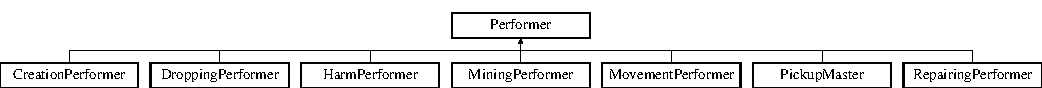
\includegraphics[height=1.185185cm]{classPerformer}
\end{center}
\end{figure}
\subsection*{Public Member Functions}
\begin{DoxyCompactItemize}
\item 
\hyperlink{classPerformer_a1674cebd080bafc7c1abf5c80afa73b1}{$\sim$\-Performer} ()
\begin{DoxyCompactList}\small\item\em Destructor. \end{DoxyCompactList}\item 
\hyperlink{classPerformer_a0c02bdbee11729e0191301de64e5020d}{Performer} ()
\begin{DoxyCompactList}\small\item\em Empty constructor. \end{DoxyCompactList}\item 
virtual void \hyperlink{classPerformer_a4cfa828ea1f9f07fd1aa9d330adfb5d5}{perform} (\hyperlink{classAction}{Action} \&action)=0
\begin{DoxyCompactList}\small\item\em Performs an action if it is possible. \end{DoxyCompactList}\end{DoxyCompactItemize}


\subsection{Detailed Description}
Class is an interface for processing messages that come from the world. 


\begin{DoxyItemize}
\item It checks if an action is possible to take place in the world and
\item performs it 
\end{DoxyItemize}

Definition at line 18 of file Performer.\-h.



\subsection{Constructor \& Destructor Documentation}
\hypertarget{classPerformer_a1674cebd080bafc7c1abf5c80afa73b1}{\index{Performer@{Performer}!$\sim$\-Performer@{$\sim$\-Performer}}
\index{$\sim$\-Performer@{$\sim$\-Performer}!Performer@{Performer}}
\subsubsection[{$\sim$\-Performer}]{\setlength{\rightskip}{0pt plus 5cm}Performer\-::$\sim$\-Performer (
\begin{DoxyParamCaption}
{}
\end{DoxyParamCaption}
)}}\label{classPerformer_a1674cebd080bafc7c1abf5c80afa73b1}


Destructor. 



Definition at line 12 of file Performer.\-cpp.

\hypertarget{classPerformer_a0c02bdbee11729e0191301de64e5020d}{\index{Performer@{Performer}!Performer@{Performer}}
\index{Performer@{Performer}!Performer@{Performer}}
\subsubsection[{Performer}]{\setlength{\rightskip}{0pt plus 5cm}Performer\-::\-Performer (
\begin{DoxyParamCaption}
{}
\end{DoxyParamCaption}
)}}\label{classPerformer_a0c02bdbee11729e0191301de64e5020d}


Empty constructor. 



Definition at line 8 of file Performer.\-cpp.



\subsection{Member Function Documentation}
\hypertarget{classPerformer_a4cfa828ea1f9f07fd1aa9d330adfb5d5}{\index{Performer@{Performer}!perform@{perform}}
\index{perform@{perform}!Performer@{Performer}}
\subsubsection[{perform}]{\setlength{\rightskip}{0pt plus 5cm}virtual void Performer\-::perform (
\begin{DoxyParamCaption}
\item[{{\bf Action} \&}]{action}
\end{DoxyParamCaption}
)\hspace{0.3cm}{\ttfamily [pure virtual]}}}\label{classPerformer_a4cfa828ea1f9f07fd1aa9d330adfb5d5}


Performs an action if it is possible. 



Implemented in \hyperlink{classMiningPerformer_abfc1f91322ab3dd52af98a4cb6e3f30b}{Mining\-Performer}, \hyperlink{classCreationPerformer_a910e6f4c9e88fde870a4ca35e01c0173}{Creation\-Performer}, \hyperlink{classDroppingPerformer_a1e3c90d034e5e6a7333484668e3c5cc4}{Dropping\-Performer}, \hyperlink{classMovementPerformer_aba62f523d2a9450a75fff98e350345b3}{Movement\-Performer}, \hyperlink{classPickupMaster_ac4ad84aace812146c5fa265b0c29c5c1}{Pickup\-Master}, \hyperlink{classRepairingPerformer_ac987420b9ac52a7f189d562a0600f51b}{Repairing\-Performer}, and \hyperlink{classHarmPerformer_a58a611a6b7cd808b9e57fb6b5123701c}{Harm\-Performer}.



The documentation for this class was generated from the following files\-:\begin{DoxyCompactItemize}
\item 
control/\-Performer/\hyperlink{Performer_8h}{Performer.\-h}\item 
control/\-Performer/\hyperlink{Performer_8cpp}{Performer.\-cpp}\end{DoxyCompactItemize}

\hypertarget{classPickupMaster}{\section{Pickup\-Master Class Reference}
\label{classPickupMaster}\index{Pickup\-Master@{Pickup\-Master}}
}


No comments.  




{\ttfamily \#include $<$Pickup\-Master.\-h$>$}

Inheritance diagram for Pickup\-Master\-:\begin{figure}[H]
\begin{center}
\leavevmode
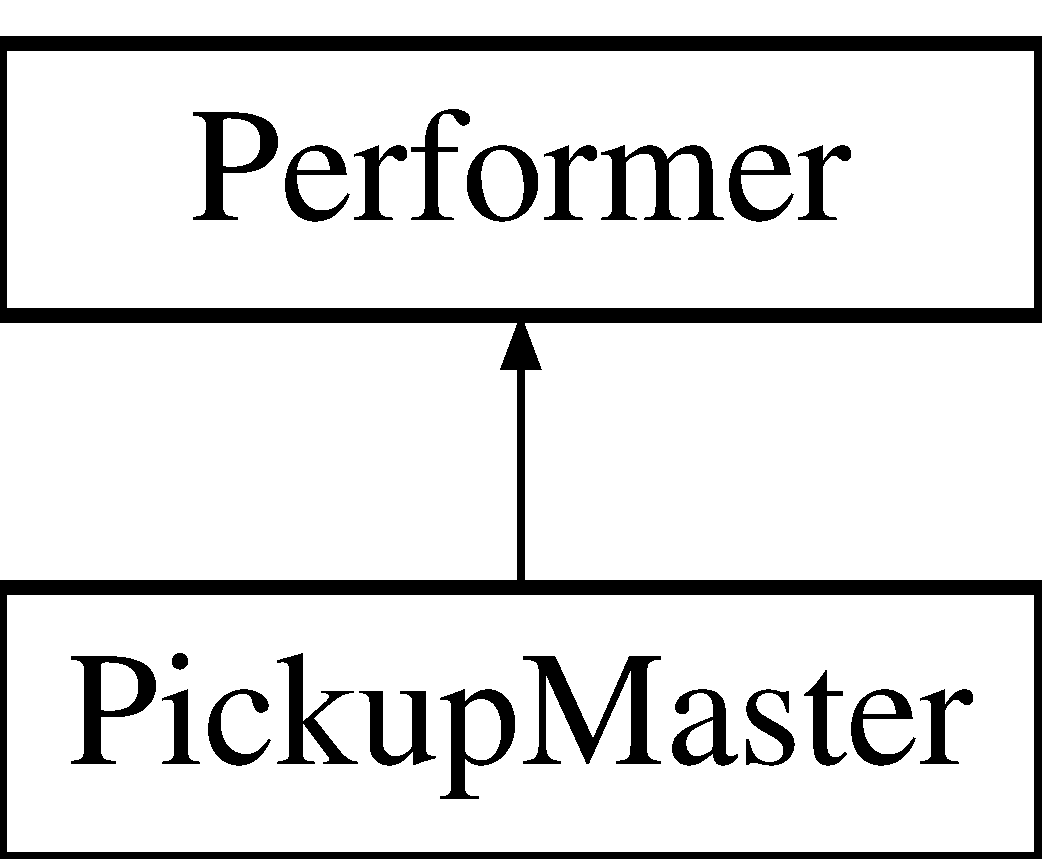
\includegraphics[height=2.000000cm]{classPickupMaster}
\end{center}
\end{figure}
\subsection*{Public Member Functions}
\begin{DoxyCompactItemize}
\item 
\hyperlink{classPickupMaster_aed62158faa3a9b869ac6f0571045fb80}{Pickup\-Master} (\hyperlink{classWorld}{World} $\ast$world)
\begin{DoxyCompactList}\small\item\em Constructor for a particular world. \end{DoxyCompactList}\item 
\hyperlink{classPickupMaster_a0202c688f4dd0a4680729420c5655092}{$\sim$\-Pickup\-Master} ()
\begin{DoxyCompactList}\small\item\em Destructor. \end{DoxyCompactList}\item 
void \hyperlink{classPickupMaster_ac4ad84aace812146c5fa265b0c29c5c1}{perform} (\hyperlink{classAction}{Action} \&action)
\begin{DoxyCompactList}\small\item\em Check if we can pick objects. \end{DoxyCompactList}\end{DoxyCompactItemize}


\subsection{Detailed Description}
No comments. 

Definition at line 16 of file Pickup\-Master.\-h.



\subsection{Constructor \& Destructor Documentation}
\hypertarget{classPickupMaster_aed62158faa3a9b869ac6f0571045fb80}{\index{Pickup\-Master@{Pickup\-Master}!Pickup\-Master@{Pickup\-Master}}
\index{Pickup\-Master@{Pickup\-Master}!PickupMaster@{Pickup\-Master}}
\subsubsection[{Pickup\-Master}]{\setlength{\rightskip}{0pt plus 5cm}Pickup\-Master\-::\-Pickup\-Master (
\begin{DoxyParamCaption}
\item[{{\bf World} $\ast$}]{world}
\end{DoxyParamCaption}
)}}\label{classPickupMaster_aed62158faa3a9b869ac6f0571045fb80}


Constructor for a particular world. 


\begin{DoxyParams}{Parameters}
{\em world\-\_\-size} & size of the world \\
\hline
{\em indexator} & indexator \\
\hline
\end{DoxyParams}


Definition at line 22 of file Pickup\-Master.\-cpp.

\hypertarget{classPickupMaster_a0202c688f4dd0a4680729420c5655092}{\index{Pickup\-Master@{Pickup\-Master}!$\sim$\-Pickup\-Master@{$\sim$\-Pickup\-Master}}
\index{$\sim$\-Pickup\-Master@{$\sim$\-Pickup\-Master}!PickupMaster@{Pickup\-Master}}
\subsubsection[{$\sim$\-Pickup\-Master}]{\setlength{\rightskip}{0pt plus 5cm}Pickup\-Master\-::$\sim$\-Pickup\-Master (
\begin{DoxyParamCaption}
{}
\end{DoxyParamCaption}
)}}\label{classPickupMaster_a0202c688f4dd0a4680729420c5655092}


Destructor. 



Definition at line 27 of file Pickup\-Master.\-cpp.



\subsection{Member Function Documentation}
\hypertarget{classPickupMaster_ac4ad84aace812146c5fa265b0c29c5c1}{\index{Pickup\-Master@{Pickup\-Master}!perform@{perform}}
\index{perform@{perform}!PickupMaster@{Pickup\-Master}}
\subsubsection[{perform}]{\setlength{\rightskip}{0pt plus 5cm}void Pickup\-Master\-::perform (
\begin{DoxyParamCaption}
\item[{{\bf Action} \&}]{action}
\end{DoxyParamCaption}
)\hspace{0.3cm}{\ttfamily [virtual]}}}\label{classPickupMaster_ac4ad84aace812146c5fa265b0c29c5c1}


Check if we can pick objects. 


\begin{DoxyParams}{Parameters}
{\em action} & a request for moving \\
\hline
\end{DoxyParams}


Implements \hyperlink{classPerformer_a4cfa828ea1f9f07fd1aa9d330adfb5d5}{Performer}.



Definition at line 31 of file Pickup\-Master.\-cpp.



The documentation for this class was generated from the following files\-:\begin{DoxyCompactItemize}
\item 
control/\-Performer/\-Pickup\-Master/\hyperlink{PickupMaster_8h}{Pickup\-Master.\-h}\item 
control/\-Performer/\-Pickup\-Master/\hyperlink{PickupMaster_8cpp}{Pickup\-Master.\-cpp}\end{DoxyCompactItemize}

\hypertarget{classPoint}{\section{Point Class Reference}
\label{classPoint}\index{Point@{Point}}
}


\hyperlink{classPoint}{Point} class.  




{\ttfamily \#include $<$Point.\-h$>$}

\subsection*{Public Member Functions}
\begin{DoxyCompactItemize}
\item 
\hyperlink{classPoint_a78b55e8d5466bb8c2cf60fa55f2562ff}{Point} (double x, double y)
\begin{DoxyCompactList}\small\item\em Constructor. \end{DoxyCompactList}\item 
\hyperlink{classPoint_ad92f2337b839a94ce97dcdb439b4325a}{Point} ()
\begin{DoxyCompactList}\small\item\em Constructor. \end{DoxyCompactList}\item 
\hyperlink{classPoint_a395fa04b4ec126b66fc053f829a30cc1}{$\sim$\-Point} ()
\begin{DoxyCompactList}\small\item\em Destructor. \end{DoxyCompactList}\item 
double \hyperlink{classPoint_a945326d198e635f9fcd0c5828b1c74c3}{get\-Distance} (const \hyperlink{classPoint}{Point} \&point) const 
\begin{DoxyCompactList}\small\item\em Compute distance to another point. \end{DoxyCompactList}\item 
double \hyperlink{classPoint_ae16c6310ac1207f57370824f70e0a3f9}{get\-Distance\-To\-Line} (const \hyperlink{classPoint}{Point} \&line\-\_\-start, const \hyperlink{classPoint}{Point} \&line\-\_\-end) const 
\begin{DoxyCompactList}\small\item\em Compute distance to a line formed by two points. \end{DoxyCompactList}\item 
bool \hyperlink{classPoint_ac05a8a1592b27bd740e3e2ec8b5b00fe}{equals} (const \hyperlink{classPoint}{Point} \&point) const 
\begin{DoxyCompactList}\small\item\em Compares two points. \end{DoxyCompactList}\item 
\hyperlink{classPoint}{Point} \hyperlink{classPoint_aa4a980a7f31a40cdf54029a3eda81dc8}{operator+} (\hyperlink{classPoint}{Point}) const 
\begin{DoxyCompactList}\small\item\em Operator +. \end{DoxyCompactList}\item 
\hyperlink{classPoint}{Point} \hyperlink{classPoint_a99f3ba7fa9ae4368a2a0ccba32aadf90}{operator-\/} (\hyperlink{classPoint}{Point}) const 
\begin{DoxyCompactList}\small\item\em Operator -\/. \end{DoxyCompactList}\item 
\hyperlink{classPoint}{Point} \& \hyperlink{classPoint_adfae003b0a76e7f55b265a33925077a9}{operator-\/=} (\hyperlink{classPoint}{Point})
\begin{DoxyCompactList}\small\item\em Operator -\/=. \end{DoxyCompactList}\item 
\hyperlink{classPoint}{Point} \& \hyperlink{classPoint_ae54aab25250505089e9d179e512b9122}{operator+=} (\hyperlink{classPoint}{Point})
\begin{DoxyCompactList}\small\item\em Operator +=. \end{DoxyCompactList}\item 
\hyperlink{classPoint}{Point} \hyperlink{classPoint_a99380b62b682c34a88713556df1287cf}{operator-\/} () const 
\begin{DoxyCompactList}\small\item\em Operator unary -\/. \end{DoxyCompactList}\item 
bool \hyperlink{classPoint_a5292afa0565b291f2c9805387caff55f}{operator==} (\hyperlink{classPoint}{Point}) const 
\begin{DoxyCompactList}\small\item\em Operator ==. \end{DoxyCompactList}\item 
bool \hyperlink{classPoint_afabdf8f492eed98971d66ef6e63a4b59}{operator!=} (\hyperlink{classPoint}{Point}) const 
\begin{DoxyCompactList}\small\item\em Operator !=. \end{DoxyCompactList}\item 
double \hyperlink{classPoint_af52a20a376f8f31e87658837565d3812}{get\-X} () const 
\begin{DoxyCompactList}\small\item\em Get X. \end{DoxyCompactList}\item 
void \hyperlink{classPoint_a9aa66c310860d038cb1258dc5cd80906}{set\-X} (double x)
\begin{DoxyCompactList}\small\item\em Set X. \end{DoxyCompactList}\item 
double \hyperlink{classPoint_aac5008459bf0e0053ce744a69187bae7}{get\-Y} () const 
\begin{DoxyCompactList}\small\item\em Get Y. \end{DoxyCompactList}\item 
void \hyperlink{classPoint_a7d1ee63237f361d41e697f87c3cb051d}{set\-Y} (double y)
\begin{DoxyCompactList}\small\item\em Set Y. \end{DoxyCompactList}\end{DoxyCompactItemize}


\subsection{Detailed Description}
\hyperlink{classPoint}{Point} class. 

Definition at line 13 of file Point.\-h.



\subsection{Constructor \& Destructor Documentation}
\hypertarget{classPoint_a78b55e8d5466bb8c2cf60fa55f2562ff}{\index{Point@{Point}!Point@{Point}}
\index{Point@{Point}!Point@{Point}}
\subsubsection[{Point}]{\setlength{\rightskip}{0pt plus 5cm}Point\-::\-Point (
\begin{DoxyParamCaption}
\item[{double}]{x, }
\item[{double}]{y}
\end{DoxyParamCaption}
)}}\label{classPoint_a78b55e8d5466bb8c2cf60fa55f2562ff}


Constructor. 


\begin{DoxyParams}{Parameters}
{\em x} & X-\/coordinate \\
\hline
{\em y} & Y-\/coordinate \\
\hline
\end{DoxyParams}


Definition at line 15 of file Point.\-cpp.

\hypertarget{classPoint_ad92f2337b839a94ce97dcdb439b4325a}{\index{Point@{Point}!Point@{Point}}
\index{Point@{Point}!Point@{Point}}
\subsubsection[{Point}]{\setlength{\rightskip}{0pt plus 5cm}Point\-::\-Point (
\begin{DoxyParamCaption}
{}
\end{DoxyParamCaption}
)}}\label{classPoint_ad92f2337b839a94ce97dcdb439b4325a}


Constructor. 



Definition at line 21 of file Point.\-cpp.

\hypertarget{classPoint_a395fa04b4ec126b66fc053f829a30cc1}{\index{Point@{Point}!$\sim$\-Point@{$\sim$\-Point}}
\index{$\sim$\-Point@{$\sim$\-Point}!Point@{Point}}
\subsubsection[{$\sim$\-Point}]{\setlength{\rightskip}{0pt plus 5cm}Point\-::$\sim$\-Point (
\begin{DoxyParamCaption}
{}
\end{DoxyParamCaption}
)}}\label{classPoint_a395fa04b4ec126b66fc053f829a30cc1}


Destructor. 



Definition at line 27 of file Point.\-cpp.



\subsection{Member Function Documentation}
\hypertarget{classPoint_ac05a8a1592b27bd740e3e2ec8b5b00fe}{\index{Point@{Point}!equals@{equals}}
\index{equals@{equals}!Point@{Point}}
\subsubsection[{equals}]{\setlength{\rightskip}{0pt plus 5cm}bool Point\-::equals (
\begin{DoxyParamCaption}
\item[{const {\bf Point} \&}]{point}
\end{DoxyParamCaption}
) const}}\label{classPoint_ac05a8a1592b27bd740e3e2ec8b5b00fe}


Compares two points. 


\begin{DoxyParams}{Parameters}
{\em point} & point to compare with \\
\hline
\end{DoxyParams}
\begin{DoxyReturn}{Returns}
true or false 
\end{DoxyReturn}


Definition at line 56 of file Point.\-cpp.

\hypertarget{classPoint_a945326d198e635f9fcd0c5828b1c74c3}{\index{Point@{Point}!get\-Distance@{get\-Distance}}
\index{get\-Distance@{get\-Distance}!Point@{Point}}
\subsubsection[{get\-Distance}]{\setlength{\rightskip}{0pt plus 5cm}double Point\-::get\-Distance (
\begin{DoxyParamCaption}
\item[{const {\bf Point} \&}]{point}
\end{DoxyParamCaption}
) const}}\label{classPoint_a945326d198e635f9fcd0c5828b1c74c3}


Compute distance to another point. 


\begin{DoxyParams}{Parameters}
{\em point} & another point \\
\hline
\end{DoxyParams}
\begin{DoxyReturn}{Returns}
distance 
\end{DoxyReturn}


Definition at line 36 of file Point.\-cpp.

\hypertarget{classPoint_ae16c6310ac1207f57370824f70e0a3f9}{\index{Point@{Point}!get\-Distance\-To\-Line@{get\-Distance\-To\-Line}}
\index{get\-Distance\-To\-Line@{get\-Distance\-To\-Line}!Point@{Point}}
\subsubsection[{get\-Distance\-To\-Line}]{\setlength{\rightskip}{0pt plus 5cm}double Point\-::get\-Distance\-To\-Line (
\begin{DoxyParamCaption}
\item[{const {\bf Point} \&}]{line\-\_\-start, }
\item[{const {\bf Point} \&}]{line\-\_\-end}
\end{DoxyParamCaption}
) const}}\label{classPoint_ae16c6310ac1207f57370824f70e0a3f9}


Compute distance to a line formed by two points. 


\begin{DoxyParams}{Parameters}
{\em line\-\_\-start} & first point of the line \\
\hline
{\em line\-\_\-end} & second point of the line \\
\hline
\end{DoxyParams}
\begin{DoxyReturn}{Returns}
distance 
\end{DoxyReturn}


Definition at line 43 of file Point.\-cpp.

\hypertarget{classPoint_af52a20a376f8f31e87658837565d3812}{\index{Point@{Point}!get\-X@{get\-X}}
\index{get\-X@{get\-X}!Point@{Point}}
\subsubsection[{get\-X}]{\setlength{\rightskip}{0pt plus 5cm}double Point\-::get\-X (
\begin{DoxyParamCaption}
{}
\end{DoxyParamCaption}
) const}}\label{classPoint_af52a20a376f8f31e87658837565d3812}


Get X. 



Definition at line 109 of file Point.\-cpp.

\hypertarget{classPoint_aac5008459bf0e0053ce744a69187bae7}{\index{Point@{Point}!get\-Y@{get\-Y}}
\index{get\-Y@{get\-Y}!Point@{Point}}
\subsubsection[{get\-Y}]{\setlength{\rightskip}{0pt plus 5cm}double Point\-::get\-Y (
\begin{DoxyParamCaption}
{}
\end{DoxyParamCaption}
) const}}\label{classPoint_aac5008459bf0e0053ce744a69187bae7}


Get Y. 



Definition at line 114 of file Point.\-cpp.

\hypertarget{classPoint_afabdf8f492eed98971d66ef6e63a4b59}{\index{Point@{Point}!operator!=@{operator!=}}
\index{operator!=@{operator!=}!Point@{Point}}
\subsubsection[{operator!=}]{\setlength{\rightskip}{0pt plus 5cm}bool Point\-::operator!= (
\begin{DoxyParamCaption}
\item[{{\bf Point}}]{point}
\end{DoxyParamCaption}
) const}}\label{classPoint_afabdf8f492eed98971d66ef6e63a4b59}


Operator !=. 



Definition at line 95 of file Point.\-cpp.

\hypertarget{classPoint_aa4a980a7f31a40cdf54029a3eda81dc8}{\index{Point@{Point}!operator+@{operator+}}
\index{operator+@{operator+}!Point@{Point}}
\subsubsection[{operator+}]{\setlength{\rightskip}{0pt plus 5cm}{\bf Point} Point\-::operator+ (
\begin{DoxyParamCaption}
\item[{{\bf Point}}]{point}
\end{DoxyParamCaption}
) const}}\label{classPoint_aa4a980a7f31a40cdf54029a3eda81dc8}


Operator +. 



Definition at line 66 of file Point.\-cpp.

\hypertarget{classPoint_ae54aab25250505089e9d179e512b9122}{\index{Point@{Point}!operator+=@{operator+=}}
\index{operator+=@{operator+=}!Point@{Point}}
\subsubsection[{operator+=}]{\setlength{\rightskip}{0pt plus 5cm}{\bf Point} \& Point\-::operator+= (
\begin{DoxyParamCaption}
\item[{{\bf Point}}]{point}
\end{DoxyParamCaption}
)}}\label{classPoint_ae54aab25250505089e9d179e512b9122}


Operator +=. 



Definition at line 83 of file Point.\-cpp.

\hypertarget{classPoint_a99f3ba7fa9ae4368a2a0ccba32aadf90}{\index{Point@{Point}!operator-\/@{operator-\/}}
\index{operator-\/@{operator-\/}!Point@{Point}}
\subsubsection[{operator-\/}]{\setlength{\rightskip}{0pt plus 5cm}{\bf Point} Point\-::operator-\/ (
\begin{DoxyParamCaption}
\item[{{\bf Point}}]{point}
\end{DoxyParamCaption}
) const}}\label{classPoint_a99f3ba7fa9ae4368a2a0ccba32aadf90}


Operator -\/. 



Definition at line 71 of file Point.\-cpp.

\hypertarget{classPoint_a99380b62b682c34a88713556df1287cf}{\index{Point@{Point}!operator-\/@{operator-\/}}
\index{operator-\/@{operator-\/}!Point@{Point}}
\subsubsection[{operator-\/}]{\setlength{\rightskip}{0pt plus 5cm}{\bf Point} Point\-::operator-\/ (
\begin{DoxyParamCaption}
{}
\end{DoxyParamCaption}
) const}}\label{classPoint_a99380b62b682c34a88713556df1287cf}


Operator unary -\/. 



Definition at line 100 of file Point.\-cpp.

\hypertarget{classPoint_adfae003b0a76e7f55b265a33925077a9}{\index{Point@{Point}!operator-\/=@{operator-\/=}}
\index{operator-\/=@{operator-\/=}!Point@{Point}}
\subsubsection[{operator-\/=}]{\setlength{\rightskip}{0pt plus 5cm}{\bf Point} \& Point\-::operator-\/= (
\begin{DoxyParamCaption}
\item[{{\bf Point}}]{point}
\end{DoxyParamCaption}
)}}\label{classPoint_adfae003b0a76e7f55b265a33925077a9}


Operator -\/=. 



Definition at line 76 of file Point.\-cpp.

\hypertarget{classPoint_a5292afa0565b291f2c9805387caff55f}{\index{Point@{Point}!operator==@{operator==}}
\index{operator==@{operator==}!Point@{Point}}
\subsubsection[{operator==}]{\setlength{\rightskip}{0pt plus 5cm}bool Point\-::operator== (
\begin{DoxyParamCaption}
\item[{{\bf Point}}]{point}
\end{DoxyParamCaption}
) const}}\label{classPoint_a5292afa0565b291f2c9805387caff55f}


Operator ==. 



Definition at line 90 of file Point.\-cpp.

\hypertarget{classPoint_a9aa66c310860d038cb1258dc5cd80906}{\index{Point@{Point}!set\-X@{set\-X}}
\index{set\-X@{set\-X}!Point@{Point}}
\subsubsection[{set\-X}]{\setlength{\rightskip}{0pt plus 5cm}void Point\-::set\-X (
\begin{DoxyParamCaption}
\item[{double}]{x}
\end{DoxyParamCaption}
)}}\label{classPoint_a9aa66c310860d038cb1258dc5cd80906}


Set X. 



Definition at line 119 of file Point.\-cpp.

\hypertarget{classPoint_a7d1ee63237f361d41e697f87c3cb051d}{\index{Point@{Point}!set\-Y@{set\-Y}}
\index{set\-Y@{set\-Y}!Point@{Point}}
\subsubsection[{set\-Y}]{\setlength{\rightskip}{0pt plus 5cm}void Point\-::set\-Y (
\begin{DoxyParamCaption}
\item[{double}]{y}
\end{DoxyParamCaption}
)}}\label{classPoint_a7d1ee63237f361d41e697f87c3cb051d}


Set Y. 



Definition at line 124 of file Point.\-cpp.



The documentation for this class was generated from the following files\-:\begin{DoxyCompactItemize}
\item 
model/\-Utilities/\-Point/\hyperlink{Point_8h}{Point.\-h}\item 
model/\-Utilities/\-Point/\hyperlink{Point_8cpp}{Point.\-cpp}\end{DoxyCompactItemize}

\hypertarget{classRepairingPerformer}{\section{Repairing\-Performer Class Reference}
\label{classRepairingPerformer}\index{Repairing\-Performer@{Repairing\-Performer}}
}


Performs a repair if it is possible.  




{\ttfamily \#include $<$Repairing\-Performer.\-h$>$}

Inheritance diagram for Repairing\-Performer\-:\begin{figure}[H]
\begin{center}
\leavevmode
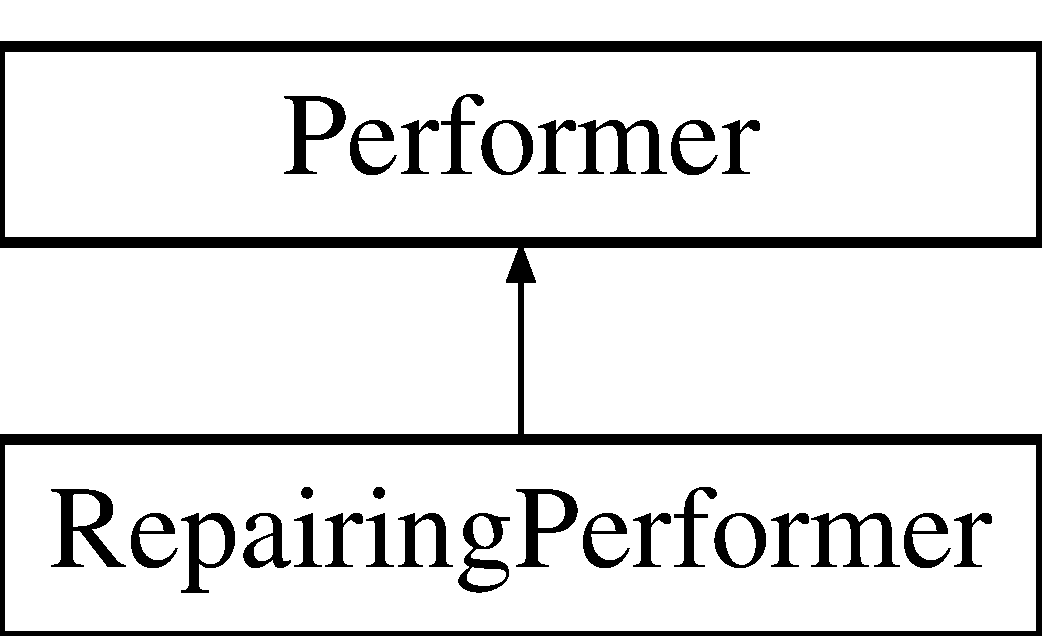
\includegraphics[height=2.000000cm]{classRepairingPerformer}
\end{center}
\end{figure}
\subsection*{Public Member Functions}
\begin{DoxyCompactItemize}
\item 
\hyperlink{classRepairingPerformer_a00372c85d083e2802071a7df02d8de9c}{Repairing\-Performer} ()
\begin{DoxyCompactList}\small\item\em Constructor. \end{DoxyCompactList}\item 
\hyperlink{classRepairingPerformer_ae0f76f761525ea03700cc62d1f895316}{$\sim$\-Repairing\-Performer} ()
\begin{DoxyCompactList}\small\item\em Destructor. \end{DoxyCompactList}\item 
void \hyperlink{classRepairingPerformer_ac987420b9ac52a7f189d562a0600f51b}{perform} (\hyperlink{classAction}{Action} \&action)
\begin{DoxyCompactList}\small\item\em Check if an object can repair and repair it. \end{DoxyCompactList}\end{DoxyCompactItemize}


\subsection{Detailed Description}
Performs a repair if it is possible. 

Definition at line 17 of file Repairing\-Performer.\-h.



\subsection{Constructor \& Destructor Documentation}
\hypertarget{classRepairingPerformer_a00372c85d083e2802071a7df02d8de9c}{\index{Repairing\-Performer@{Repairing\-Performer}!Repairing\-Performer@{Repairing\-Performer}}
\index{Repairing\-Performer@{Repairing\-Performer}!RepairingPerformer@{Repairing\-Performer}}
\subsubsection[{Repairing\-Performer}]{\setlength{\rightskip}{0pt plus 5cm}Repairing\-Performer\-::\-Repairing\-Performer (
\begin{DoxyParamCaption}
{}
\end{DoxyParamCaption}
)}}\label{classRepairingPerformer_a00372c85d083e2802071a7df02d8de9c}


Constructor. 



Definition at line 8 of file Repairing\-Performer.\-cpp.

\hypertarget{classRepairingPerformer_ae0f76f761525ea03700cc62d1f895316}{\index{Repairing\-Performer@{Repairing\-Performer}!$\sim$\-Repairing\-Performer@{$\sim$\-Repairing\-Performer}}
\index{$\sim$\-Repairing\-Performer@{$\sim$\-Repairing\-Performer}!RepairingPerformer@{Repairing\-Performer}}
\subsubsection[{$\sim$\-Repairing\-Performer}]{\setlength{\rightskip}{0pt plus 5cm}Repairing\-Performer\-::$\sim$\-Repairing\-Performer (
\begin{DoxyParamCaption}
{}
\end{DoxyParamCaption}
)}}\label{classRepairingPerformer_ae0f76f761525ea03700cc62d1f895316}


Destructor. 



Definition at line 13 of file Repairing\-Performer.\-cpp.



\subsection{Member Function Documentation}
\hypertarget{classRepairingPerformer_ac987420b9ac52a7f189d562a0600f51b}{\index{Repairing\-Performer@{Repairing\-Performer}!perform@{perform}}
\index{perform@{perform}!RepairingPerformer@{Repairing\-Performer}}
\subsubsection[{perform}]{\setlength{\rightskip}{0pt plus 5cm}void Repairing\-Performer\-::perform (
\begin{DoxyParamCaption}
\item[{{\bf Action} \&}]{action}
\end{DoxyParamCaption}
)\hspace{0.3cm}{\ttfamily [virtual]}}}\label{classRepairingPerformer_ac987420b9ac52a7f189d562a0600f51b}


Check if an object can repair and repair it. 


\begin{DoxyParams}{Parameters}
{\em action} & a request for repairing \\
\hline
\end{DoxyParams}


Implements \hyperlink{classPerformer_a4cfa828ea1f9f07fd1aa9d330adfb5d5}{Performer}.



Definition at line 18 of file Repairing\-Performer.\-cpp.



The documentation for this class was generated from the following files\-:\begin{DoxyCompactItemize}
\item 
control/\-Performer/\-Repairing\-Performer/\hyperlink{RepairingPerformer_8h}{Repairing\-Performer.\-h}\item 
control/\-Performer/\-Repairing\-Performer/\hyperlink{RepairingPerformer_8cpp}{Repairing\-Performer.\-cpp}\end{DoxyCompactItemize}

\hypertarget{classResource}{\section{Resource Class Reference}
\label{classResource}\index{Resource@{Resource}}
}


This class contains information about mineable or pickable resource.  




{\ttfamily \#include $<$Resource.\-h$>$}

Inheritance diagram for Resource\-:\begin{figure}[H]
\begin{center}
\leavevmode
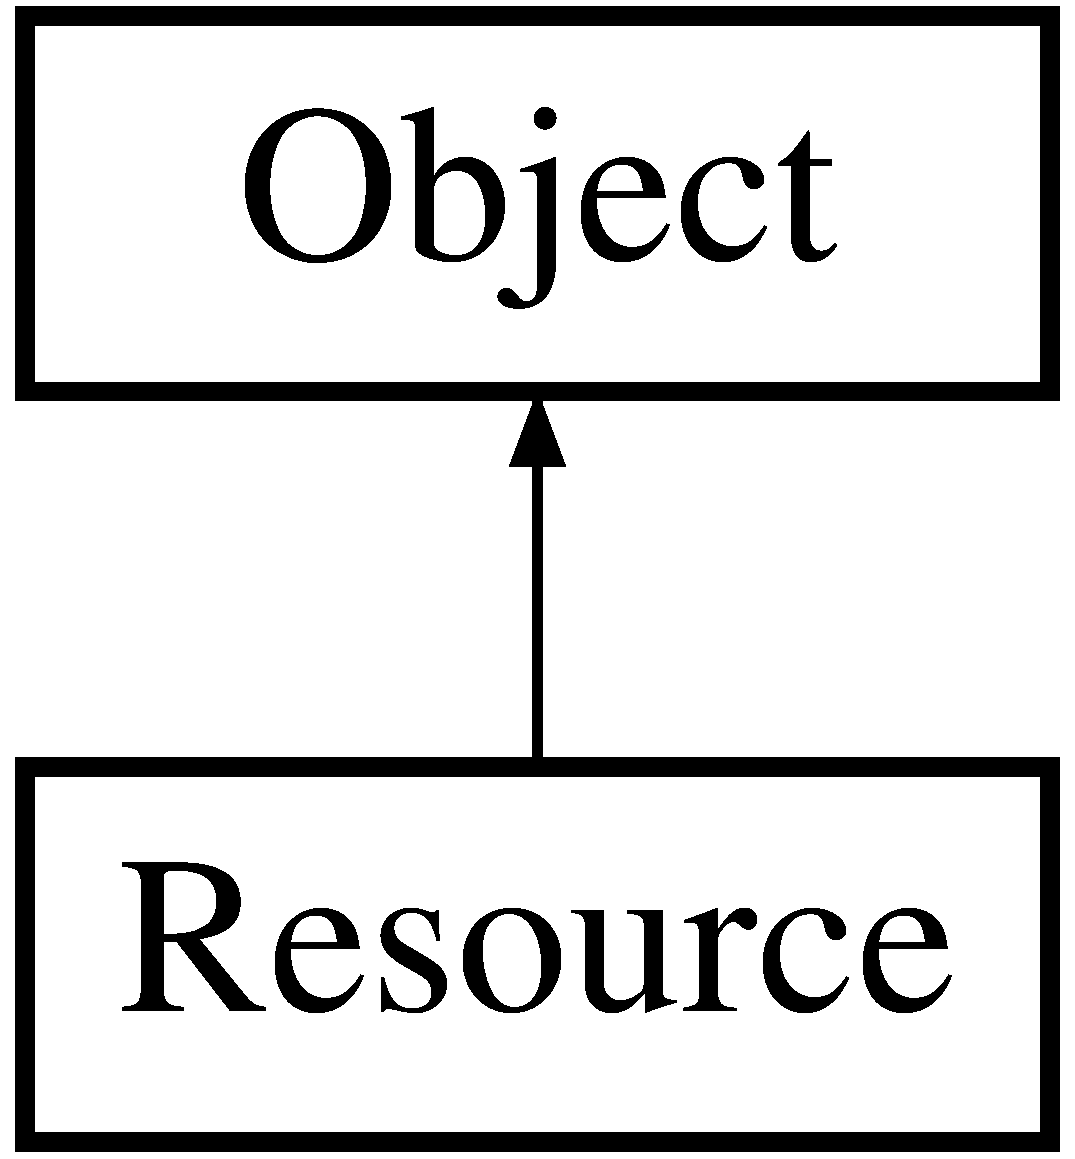
\includegraphics[height=2.000000cm]{classResource}
\end{center}
\end{figure}
\subsection*{Public Member Functions}
\begin{DoxyCompactItemize}
\item 
\hyperlink{classResource_a5740e20b90ce4cc9dd8cdb96947bd298}{Resource} (\hyperlink{BasicTypes_8h_a8571efa4409be32e28abf3ea74a0dbb1}{Resource\-Type} type, \hyperlink{BasicTypes_8h_a91ad9478d81a7aaf2593e8d9c3d06a14}{uint} res\-\_\-amount=0)
\begin{DoxyCompactList}\small\item\em Constructor. \end{DoxyCompactList}\item 
virtual \hyperlink{classResource_a0e5ec475e2601bdb33644468e86f6f10}{$\sim$\-Resource} ()
\begin{DoxyCompactList}\small\item\em Destructor. \end{DoxyCompactList}\item 
void \hyperlink{classResource_a6eb73f19cd1f3cf7485dc659256fe239}{increment\-Progress} ()
\begin{DoxyCompactList}\small\item\em Increment progress of mining by one. \end{DoxyCompactList}\item 
void \hyperlink{classResource_acb41587e4354c39a81c4f7d2674f4f88}{decrease\-Amount} (\hyperlink{BasicTypes_8h_a91ad9478d81a7aaf2593e8d9c3d06a14}{uint} delta)
\begin{DoxyCompactList}\small\item\em Decreases amount of resource. \end{DoxyCompactList}\item 
void \hyperlink{classResource_a55b2623e12687bedc2efced0bc781fc6}{increase\-Amount} (\hyperlink{BasicTypes_8h_a91ad9478d81a7aaf2593e8d9c3d06a14}{uint} delta)
\begin{DoxyCompactList}\small\item\em Increases amount of resource. \end{DoxyCompactList}\item 
\hyperlink{BasicTypes_8h_a91ad9478d81a7aaf2593e8d9c3d06a14}{uint} \hyperlink{classResource_a0a83fccc63c105f0f3dd706daebb1270}{get\-Amount} () const 
\begin{DoxyCompactList}\small\item\em Gets amount of resource. \end{DoxyCompactList}\item 
void \hyperlink{classResource_aaba80262d4086bfce08ea4d4c0d63f75}{damage} (\hyperlink{BasicTypes_8h_a91ad9478d81a7aaf2593e8d9c3d06a14}{uint} delta)
\begin{DoxyCompactList}\small\item\em Damages resource. \end{DoxyCompactList}\item 
void \hyperlink{classResource_a88928f89a1a538768dade43b0493ec6c}{heal} (\hyperlink{BasicTypes_8h_a91ad9478d81a7aaf2593e8d9c3d06a14}{uint} delta)
\begin{DoxyCompactList}\small\item\em ''Heals'' resource. \end{DoxyCompactList}\item 
std\-::vector$<$ \hyperlink{classAction}{Action} $>$ $\ast$ \hyperlink{classResource_a4c4cc169461d76de8787c97276665168}{get\-Actions} ()
\begin{DoxyCompactList}\small\item\em Gets array with pending actions. \end{DoxyCompactList}\item 
\hyperlink{BasicTypes_8h_a8571efa4409be32e28abf3ea74a0dbb1}{Resource\-Type} \hyperlink{classResource_ae3b7847e943a7b82f90bcf32ecd1e797}{get\-Subtype} () const 
\begin{DoxyCompactList}\small\item\em Gets the value of subtype. \end{DoxyCompactList}\item 
\hyperlink{BasicTypes_8h_a91ad9478d81a7aaf2593e8d9c3d06a14}{uint} \hyperlink{classResource_a512a227f9ddfaf59d40cf878dbf6c937}{get\-Progress} () const 
\begin{DoxyCompactList}\small\item\em Get the value of progress. \end{DoxyCompactList}\item 
\hyperlink{BasicTypes_8h_a91ad9478d81a7aaf2593e8d9c3d06a14}{uint} \hyperlink{classResource_a0b6ea6582c309b2db3c57274b687e7d2}{get\-Difficulty} () const 
\begin{DoxyCompactList}\small\item\em Get the value of difficulty. \end{DoxyCompactList}\item 
bool \hyperlink{classResource_ad87877637e96514ddefed5cae8adaa99}{is\-Mineable} () const 
\begin{DoxyCompactList}\small\item\em Returns true if resource is mineable. \end{DoxyCompactList}\end{DoxyCompactItemize}
\subsection*{Additional Inherited Members}


\subsection{Detailed Description}
This class contains information about mineable or pickable resource. 

Definition at line 17 of file Resource.\-h.



\subsection{Constructor \& Destructor Documentation}
\hypertarget{classResource_a5740e20b90ce4cc9dd8cdb96947bd298}{\index{Resource@{Resource}!Resource@{Resource}}
\index{Resource@{Resource}!Resource@{Resource}}
\subsubsection[{Resource}]{\setlength{\rightskip}{0pt plus 5cm}Resource\-::\-Resource (
\begin{DoxyParamCaption}
\item[{{\bf Resource\-Type}}]{type, }
\item[{{\bf uint}}]{res\-\_\-amount = {\ttfamily 0}}
\end{DoxyParamCaption}
)}}\label{classResource_a5740e20b90ce4cc9dd8cdb96947bd298}


Constructor. 



Definition at line 15 of file Resource.\-cpp.

\hypertarget{classResource_a0e5ec475e2601bdb33644468e86f6f10}{\index{Resource@{Resource}!$\sim$\-Resource@{$\sim$\-Resource}}
\index{$\sim$\-Resource@{$\sim$\-Resource}!Resource@{Resource}}
\subsubsection[{$\sim$\-Resource}]{\setlength{\rightskip}{0pt plus 5cm}Resource\-::$\sim$\-Resource (
\begin{DoxyParamCaption}
{}
\end{DoxyParamCaption}
)\hspace{0.3cm}{\ttfamily [virtual]}}}\label{classResource_a0e5ec475e2601bdb33644468e86f6f10}


Destructor. 



Definition at line 77 of file Resource.\-cpp.



\subsection{Member Function Documentation}
\hypertarget{classResource_aaba80262d4086bfce08ea4d4c0d63f75}{\index{Resource@{Resource}!damage@{damage}}
\index{damage@{damage}!Resource@{Resource}}
\subsubsection[{damage}]{\setlength{\rightskip}{0pt plus 5cm}void Resource\-::damage (
\begin{DoxyParamCaption}
\item[{{\bf uint}}]{delta}
\end{DoxyParamCaption}
)\hspace{0.3cm}{\ttfamily [virtual]}}}\label{classResource_aaba80262d4086bfce08ea4d4c0d63f75}


Damages resource. 


\begin{DoxyParams}{Parameters}
{\em delta} & amount of damage \\
\hline
\end{DoxyParams}


Implements \hyperlink{classObject_a816838bab5c67fce2cead6cb9122ad47}{Object}.



Definition at line 117 of file Resource.\-cpp.

\hypertarget{classResource_acb41587e4354c39a81c4f7d2674f4f88}{\index{Resource@{Resource}!decrease\-Amount@{decrease\-Amount}}
\index{decrease\-Amount@{decrease\-Amount}!Resource@{Resource}}
\subsubsection[{decrease\-Amount}]{\setlength{\rightskip}{0pt plus 5cm}void Resource\-::decrease\-Amount (
\begin{DoxyParamCaption}
\item[{{\bf uint}}]{delta}
\end{DoxyParamCaption}
)}}\label{classResource_acb41587e4354c39a81c4f7d2674f4f88}


Decreases amount of resource. 


\begin{DoxyParams}{Parameters}
{\em delta} & amount of resource to decrease \\
\hline
\end{DoxyParams}


Definition at line 94 of file Resource.\-cpp.

\hypertarget{classResource_a4c4cc169461d76de8787c97276665168}{\index{Resource@{Resource}!get\-Actions@{get\-Actions}}
\index{get\-Actions@{get\-Actions}!Resource@{Resource}}
\subsubsection[{get\-Actions}]{\setlength{\rightskip}{0pt plus 5cm}std\-::vector$<$ {\bf Action} $>$ $\ast$ Resource\-::get\-Actions (
\begin{DoxyParamCaption}
{}
\end{DoxyParamCaption}
)\hspace{0.3cm}{\ttfamily [virtual]}}}\label{classResource_a4c4cc169461d76de8787c97276665168}


Gets array with pending actions. 

\begin{DoxyReturn}{Returns}
array with pending actions 
\end{DoxyReturn}


Implements \hyperlink{classObject_addf0658ee2f8da579d10a6682dc097d7}{Object}.



Definition at line 131 of file Resource.\-cpp.

\hypertarget{classResource_a0a83fccc63c105f0f3dd706daebb1270}{\index{Resource@{Resource}!get\-Amount@{get\-Amount}}
\index{get\-Amount@{get\-Amount}!Resource@{Resource}}
\subsubsection[{get\-Amount}]{\setlength{\rightskip}{0pt plus 5cm}{\bf uint} Resource\-::get\-Amount (
\begin{DoxyParamCaption}
{}
\end{DoxyParamCaption}
) const}}\label{classResource_a0a83fccc63c105f0f3dd706daebb1270}


Gets amount of resource. 

\begin{DoxyReturn}{Returns}
amount of resource 
\end{DoxyReturn}


Definition at line 112 of file Resource.\-cpp.

\hypertarget{classResource_a0b6ea6582c309b2db3c57274b687e7d2}{\index{Resource@{Resource}!get\-Difficulty@{get\-Difficulty}}
\index{get\-Difficulty@{get\-Difficulty}!Resource@{Resource}}
\subsubsection[{get\-Difficulty}]{\setlength{\rightskip}{0pt plus 5cm}{\bf uint} Resource\-::get\-Difficulty (
\begin{DoxyParamCaption}
{}
\end{DoxyParamCaption}
) const}}\label{classResource_a0b6ea6582c309b2db3c57274b687e7d2}


Get the value of difficulty. 

\begin{DoxyReturn}{Returns}
the value of difficulty 
\end{DoxyReturn}


Definition at line 186 of file Resource.\-cpp.

\hypertarget{classResource_a512a227f9ddfaf59d40cf878dbf6c937}{\index{Resource@{Resource}!get\-Progress@{get\-Progress}}
\index{get\-Progress@{get\-Progress}!Resource@{Resource}}
\subsubsection[{get\-Progress}]{\setlength{\rightskip}{0pt plus 5cm}{\bf uint} Resource\-::get\-Progress (
\begin{DoxyParamCaption}
{}
\end{DoxyParamCaption}
) const}}\label{classResource_a512a227f9ddfaf59d40cf878dbf6c937}


Get the value of progress. 

\begin{DoxyReturn}{Returns}
the value of progress 
\end{DoxyReturn}


Definition at line 181 of file Resource.\-cpp.

\hypertarget{classResource_ae3b7847e943a7b82f90bcf32ecd1e797}{\index{Resource@{Resource}!get\-Subtype@{get\-Subtype}}
\index{get\-Subtype@{get\-Subtype}!Resource@{Resource}}
\subsubsection[{get\-Subtype}]{\setlength{\rightskip}{0pt plus 5cm}{\bf Resource\-Type} Resource\-::get\-Subtype (
\begin{DoxyParamCaption}
{}
\end{DoxyParamCaption}
) const}}\label{classResource_ae3b7847e943a7b82f90bcf32ecd1e797}


Gets the value of subtype. 

\begin{DoxyReturn}{Returns}
the value of subtype 
\end{DoxyReturn}


Definition at line 172 of file Resource.\-cpp.

\hypertarget{classResource_a88928f89a1a538768dade43b0493ec6c}{\index{Resource@{Resource}!heal@{heal}}
\index{heal@{heal}!Resource@{Resource}}
\subsubsection[{heal}]{\setlength{\rightskip}{0pt plus 5cm}void Resource\-::heal (
\begin{DoxyParamCaption}
\item[{{\bf uint}}]{delta}
\end{DoxyParamCaption}
)\hspace{0.3cm}{\ttfamily [virtual]}}}\label{classResource_a88928f89a1a538768dade43b0493ec6c}


''Heals'' resource. 


\begin{DoxyParams}{Parameters}
{\em delta} & amount of healing points \\
\hline
\end{DoxyParams}


Implements \hyperlink{classObject_af7f49cb3f3c3bd9cfdbc42beecbbe5bc}{Object}.



Definition at line 122 of file Resource.\-cpp.

\hypertarget{classResource_a55b2623e12687bedc2efced0bc781fc6}{\index{Resource@{Resource}!increase\-Amount@{increase\-Amount}}
\index{increase\-Amount@{increase\-Amount}!Resource@{Resource}}
\subsubsection[{increase\-Amount}]{\setlength{\rightskip}{0pt plus 5cm}void Resource\-::increase\-Amount (
\begin{DoxyParamCaption}
\item[{{\bf uint}}]{delta}
\end{DoxyParamCaption}
)}}\label{classResource_a55b2623e12687bedc2efced0bc781fc6}


Increases amount of resource. 


\begin{DoxyParams}{Parameters}
{\em delta} & amount of resource to increase \\
\hline
\end{DoxyParams}


Definition at line 106 of file Resource.\-cpp.

\hypertarget{classResource_a6eb73f19cd1f3cf7485dc659256fe239}{\index{Resource@{Resource}!increment\-Progress@{increment\-Progress}}
\index{increment\-Progress@{increment\-Progress}!Resource@{Resource}}
\subsubsection[{increment\-Progress}]{\setlength{\rightskip}{0pt plus 5cm}void Resource\-::increment\-Progress (
\begin{DoxyParamCaption}
{}
\end{DoxyParamCaption}
)}}\label{classResource_a6eb73f19cd1f3cf7485dc659256fe239}


Increment progress of mining by one. 



Definition at line 85 of file Resource.\-cpp.

\hypertarget{classResource_ad87877637e96514ddefed5cae8adaa99}{\index{Resource@{Resource}!is\-Mineable@{is\-Mineable}}
\index{is\-Mineable@{is\-Mineable}!Resource@{Resource}}
\subsubsection[{is\-Mineable}]{\setlength{\rightskip}{0pt plus 5cm}bool Resource\-::is\-Mineable (
\begin{DoxyParamCaption}
{}
\end{DoxyParamCaption}
) const}}\label{classResource_ad87877637e96514ddefed5cae8adaa99}


Returns true if resource is mineable. 

\begin{DoxyReturn}{Returns}
is mineable or not 
\end{DoxyReturn}


Definition at line 191 of file Resource.\-cpp.



The documentation for this class was generated from the following files\-:\begin{DoxyCompactItemize}
\item 
model/\-World/\-Object/\-Resource/\hyperlink{Resource_8h}{Resource.\-h}\item 
model/\-World/\-Object/\-Resource/\hyperlink{Resource_8cpp}{Resource.\-cpp}\end{DoxyCompactItemize}

\hypertarget{classShape}{\section{Shape Class Reference}
\label{classShape}\index{Shape@{Shape}}
}


{\ttfamily \#include $<$Shape.\-h$>$}

\subsection*{Public Member Functions}
\begin{DoxyCompactItemize}
\item 
\hyperlink{classShape_a8e8680c7a68edeb2826e9e72cfa9adbf}{Shape} (\hyperlink{classPoint}{Point} center, int type, double size)
\begin{DoxyCompactList}\small\item\em Constructor. \end{DoxyCompactList}\item 
\hyperlink{classShape_aaa8d87171e65e0d8ba3c5459978992a7}{Shape} ()
\begin{DoxyCompactList}\small\item\em Constructor. \end{DoxyCompactList}\item 
\hyperlink{classShape_a935afc9e576015f967d90de56977167d}{$\sim$\-Shape} ()
\begin{DoxyCompactList}\small\item\em Destructor. \end{DoxyCompactList}\item 
void \hyperlink{classShape_aabf2fde36d48854cb10fbae4fe6ea0cf}{set\-Center} (\hyperlink{classPoint}{Point} new\-\_\-var)
\begin{DoxyCompactList}\small\item\em Set the value of center. \end{DoxyCompactList}\item 
const \hyperlink{classPoint}{Point} \& \hyperlink{classShape_a178ba40bdc7f20c1342f34450257f740}{get\-Center} () const 
\begin{DoxyCompactList}\small\item\em Get the value of center. \end{DoxyCompactList}\item 
int \hyperlink{classShape_ace78f87ad50bac4ea2592e730a7e9630}{get\-Type} () const 
\begin{DoxyCompactList}\small\item\em Get type of the shape. \end{DoxyCompactList}\item 
void \hyperlink{classShape_a44bfca3ef6564ff0f34badc77f594862}{set\-Type} (int type)
\begin{DoxyCompactList}\small\item\em Set type. \end{DoxyCompactList}\item 
double \hyperlink{classShape_a1c04ad00113b2a8c0787c50edfa08c5c}{get\-Size} () const 
\begin{DoxyCompactList}\small\item\em Get size (edge length for polygons, diameter for circle). \end{DoxyCompactList}\item 
void \hyperlink{classShape_aaee049351828e1209697bb2b357ca61a}{set\-Size} (double size)
\begin{DoxyCompactList}\small\item\em Set size (edge length for polygons, radius for circle). \end{DoxyCompactList}\item 
\hyperlink{classPoint}{Point} \hyperlink{classShape_ac28a20365613c955cfb3ebc3f452b6c6}{get\-Last\-Center} ()
\begin{DoxyCompactList}\small\item\em Get last position of shape. \end{DoxyCompactList}\item 
bool \hyperlink{classShape_a0ff4bb8b9d0a6e6ad47ab3b7037b0302}{hit\-Test} (const \hyperlink{classPoint}{Point} \&point) const 
\begin{DoxyCompactList}\small\item\em Tests if a \hyperlink{classShape}{Shape} includes a point. \end{DoxyCompactList}\item 
bool \hyperlink{classShape_ab545013b4a52ccc4acd7d8a56d45d5c8}{hit\-Test} (const \hyperlink{classShape}{Shape} \&shape) const 
\begin{DoxyCompactList}\small\item\em Tests if a \hyperlink{classShape}{Shape} intersects with another \hyperlink{classShape}{Shape}. \end{DoxyCompactList}\item 
int \hyperlink{classShape_ad4e614404ea0276a9eee3d8299b24e98}{intersect} (const \hyperlink{classShape}{Shape} \&shape)
\begin{DoxyCompactList}\small\item\em Get intersections of minimal bounding boxes with another shape. \end{DoxyCompactList}\item 
\hyperlink{classPoint}{Point} \hyperlink{classShape_aab4459fa7eb1ed03c052e6f5a99c231f}{get\-Left\-Bottom} () const 
\begin{DoxyCompactList}\small\item\em Gets the left bottom point of the shape. \end{DoxyCompactList}\item 
\hyperlink{classPoint}{Point} \hyperlink{classShape_a97c5436ae38f0994f0eb3b6a2c1eed08}{get\-Right\-Top} () const 
\begin{DoxyCompactList}\small\item\em Gets the right top point of the shape. \end{DoxyCompactList}\end{DoxyCompactItemize}


\subsection{Detailed Description}
class \hyperlink{classShape}{Shape} \hyperlink{classShape}{Shape} are needed for objects' bounds and view areas 

Definition at line 17 of file Shape.\-h.



\subsection{Constructor \& Destructor Documentation}
\hypertarget{classShape_a8e8680c7a68edeb2826e9e72cfa9adbf}{\index{Shape@{Shape}!Shape@{Shape}}
\index{Shape@{Shape}!Shape@{Shape}}
\subsubsection[{Shape}]{\setlength{\rightskip}{0pt plus 5cm}Shape\-::\-Shape (
\begin{DoxyParamCaption}
\item[{{\bf Point}}]{center, }
\item[{int}]{type, }
\item[{double}]{size}
\end{DoxyParamCaption}
)}}\label{classShape_a8e8680c7a68edeb2826e9e72cfa9adbf}


Constructor. 


\begin{DoxyParams}{Parameters}
{\em type} & type of the shape \\
\hline
{\em center} & center of the \hyperlink{classShape}{Shape} \\
\hline
{\em size} & size of the \hyperlink{classShape}{Shape} (edge length for polygons, diameter for circle). \\
\hline
\end{DoxyParams}


Definition at line 17 of file Shape.\-cpp.

\hypertarget{classShape_aaa8d87171e65e0d8ba3c5459978992a7}{\index{Shape@{Shape}!Shape@{Shape}}
\index{Shape@{Shape}!Shape@{Shape}}
\subsubsection[{Shape}]{\setlength{\rightskip}{0pt plus 5cm}Shape\-::\-Shape (
\begin{DoxyParamCaption}
{}
\end{DoxyParamCaption}
)}}\label{classShape_aaa8d87171e65e0d8ba3c5459978992a7}


Constructor. 



Definition at line 26 of file Shape.\-cpp.

\hypertarget{classShape_a935afc9e576015f967d90de56977167d}{\index{Shape@{Shape}!$\sim$\-Shape@{$\sim$\-Shape}}
\index{$\sim$\-Shape@{$\sim$\-Shape}!Shape@{Shape}}
\subsubsection[{$\sim$\-Shape}]{\setlength{\rightskip}{0pt plus 5cm}Shape\-::$\sim$\-Shape (
\begin{DoxyParamCaption}
{}
\end{DoxyParamCaption}
)}}\label{classShape_a935afc9e576015f967d90de56977167d}


Destructor. 



Definition at line 30 of file Shape.\-cpp.



\subsection{Member Function Documentation}
\hypertarget{classShape_a178ba40bdc7f20c1342f34450257f740}{\index{Shape@{Shape}!get\-Center@{get\-Center}}
\index{get\-Center@{get\-Center}!Shape@{Shape}}
\subsubsection[{get\-Center}]{\setlength{\rightskip}{0pt plus 5cm}const {\bf Point} \& Shape\-::get\-Center (
\begin{DoxyParamCaption}
{}
\end{DoxyParamCaption}
) const}}\label{classShape_a178ba40bdc7f20c1342f34450257f740}


Get the value of center. 

\begin{DoxyReturn}{Returns}
the value of center. 
\end{DoxyReturn}


Definition at line 44 of file Shape.\-cpp.

\hypertarget{classShape_ac28a20365613c955cfb3ebc3f452b6c6}{\index{Shape@{Shape}!get\-Last\-Center@{get\-Last\-Center}}
\index{get\-Last\-Center@{get\-Last\-Center}!Shape@{Shape}}
\subsubsection[{get\-Last\-Center}]{\setlength{\rightskip}{0pt plus 5cm}{\bf Point} Shape\-::get\-Last\-Center (
\begin{DoxyParamCaption}
{}
\end{DoxyParamCaption}
)}}\label{classShape_ac28a20365613c955cfb3ebc3f452b6c6}


Get last position of shape. 

\begin{DoxyReturn}{Returns}
coordinates of the last position 
\end{DoxyReturn}


Definition at line 96 of file Shape.\-cpp.

\hypertarget{classShape_aab4459fa7eb1ed03c052e6f5a99c231f}{\index{Shape@{Shape}!get\-Left\-Bottom@{get\-Left\-Bottom}}
\index{get\-Left\-Bottom@{get\-Left\-Bottom}!Shape@{Shape}}
\subsubsection[{get\-Left\-Bottom}]{\setlength{\rightskip}{0pt plus 5cm}{\bf Point} Shape\-::get\-Left\-Bottom (
\begin{DoxyParamCaption}
{}
\end{DoxyParamCaption}
) const}}\label{classShape_aab4459fa7eb1ed03c052e6f5a99c231f}


Gets the left bottom point of the shape. 



Definition at line 86 of file Shape.\-cpp.

\hypertarget{classShape_a97c5436ae38f0994f0eb3b6a2c1eed08}{\index{Shape@{Shape}!get\-Right\-Top@{get\-Right\-Top}}
\index{get\-Right\-Top@{get\-Right\-Top}!Shape@{Shape}}
\subsubsection[{get\-Right\-Top}]{\setlength{\rightskip}{0pt plus 5cm}{\bf Point} Shape\-::get\-Right\-Top (
\begin{DoxyParamCaption}
{}
\end{DoxyParamCaption}
) const}}\label{classShape_a97c5436ae38f0994f0eb3b6a2c1eed08}


Gets the right top point of the shape. 



Definition at line 91 of file Shape.\-cpp.

\hypertarget{classShape_a1c04ad00113b2a8c0787c50edfa08c5c}{\index{Shape@{Shape}!get\-Size@{get\-Size}}
\index{get\-Size@{get\-Size}!Shape@{Shape}}
\subsubsection[{get\-Size}]{\setlength{\rightskip}{0pt plus 5cm}double Shape\-::get\-Size (
\begin{DoxyParamCaption}
{}
\end{DoxyParamCaption}
) const}}\label{classShape_a1c04ad00113b2a8c0787c50edfa08c5c}


Get size (edge length for polygons, diameter for circle). 

\begin{DoxyReturn}{Returns}
size 
\end{DoxyReturn}


Definition at line 66 of file Shape.\-cpp.

\hypertarget{classShape_ace78f87ad50bac4ea2592e730a7e9630}{\index{Shape@{Shape}!get\-Type@{get\-Type}}
\index{get\-Type@{get\-Type}!Shape@{Shape}}
\subsubsection[{get\-Type}]{\setlength{\rightskip}{0pt plus 5cm}int Shape\-::get\-Type (
\begin{DoxyParamCaption}
{}
\end{DoxyParamCaption}
) const}}\label{classShape_ace78f87ad50bac4ea2592e730a7e9630}


Get type of the shape. 

\begin{DoxyReturn}{Returns}
type of the shape. 
\end{DoxyReturn}


Definition at line 54 of file Shape.\-cpp.

\hypertarget{classShape_a0ff4bb8b9d0a6e6ad47ab3b7037b0302}{\index{Shape@{Shape}!hit\-Test@{hit\-Test}}
\index{hit\-Test@{hit\-Test}!Shape@{Shape}}
\subsubsection[{hit\-Test}]{\setlength{\rightskip}{0pt plus 5cm}bool Shape\-::hit\-Test (
\begin{DoxyParamCaption}
\item[{const {\bf Point} \&}]{point}
\end{DoxyParamCaption}
) const}}\label{classShape_a0ff4bb8b9d0a6e6ad47ab3b7037b0302}


Tests if a \hyperlink{classShape}{Shape} includes a point. 

\begin{DoxyReturn}{Returns}
true or false 
\end{DoxyReturn}

\begin{DoxyParams}{Parameters}
{\em point} & point to test \\
\hline
\end{DoxyParams}


Definition at line 106 of file Shape.\-cpp.

\hypertarget{classShape_ab545013b4a52ccc4acd7d8a56d45d5c8}{\index{Shape@{Shape}!hit\-Test@{hit\-Test}}
\index{hit\-Test@{hit\-Test}!Shape@{Shape}}
\subsubsection[{hit\-Test}]{\setlength{\rightskip}{0pt plus 5cm}bool Shape\-::hit\-Test (
\begin{DoxyParamCaption}
\item[{const {\bf Shape} \&}]{shape}
\end{DoxyParamCaption}
) const}}\label{classShape_ab545013b4a52ccc4acd7d8a56d45d5c8}


Tests if a \hyperlink{classShape}{Shape} intersects with another \hyperlink{classShape}{Shape}. 

\begin{DoxyReturn}{Returns}
true or false 
\end{DoxyReturn}

\begin{DoxyParams}{Parameters}
{\em shape} & \hyperlink{classShape}{Shape} to test \\
\hline
\end{DoxyParams}


Definition at line 132 of file Shape.\-cpp.

\hypertarget{classShape_ad4e614404ea0276a9eee3d8299b24e98}{\index{Shape@{Shape}!intersect@{intersect}}
\index{intersect@{intersect}!Shape@{Shape}}
\subsubsection[{intersect}]{\setlength{\rightskip}{0pt plus 5cm}int Shape\-::intersect (
\begin{DoxyParamCaption}
\item[{const {\bf Shape} \&}]{shape}
\end{DoxyParamCaption}
)}}\label{classShape_ad4e614404ea0276a9eee3d8299b24e98}


Get intersections of minimal bounding boxes with another shape. 


\begin{DoxyParams}{Parameters}
{\em shape} & another shape \\
\hline
\end{DoxyParams}
\begin{DoxyReturn}{Returns}
flags of intersections 
\end{DoxyReturn}


Definition at line 250 of file Shape.\-cpp.

\hypertarget{classShape_aabf2fde36d48854cb10fbae4fe6ea0cf}{\index{Shape@{Shape}!set\-Center@{set\-Center}}
\index{set\-Center@{set\-Center}!Shape@{Shape}}
\subsubsection[{set\-Center}]{\setlength{\rightskip}{0pt plus 5cm}void Shape\-::set\-Center (
\begin{DoxyParamCaption}
\item[{{\bf Point}}]{new\-\_\-var}
\end{DoxyParamCaption}
)}}\label{classShape_aabf2fde36d48854cb10fbae4fe6ea0cf}


Set the value of center. 


\begin{DoxyParams}{Parameters}
{\em new\-\_\-var} & the new value of center. \\
\hline
\end{DoxyParams}


Definition at line 38 of file Shape.\-cpp.

\hypertarget{classShape_aaee049351828e1209697bb2b357ca61a}{\index{Shape@{Shape}!set\-Size@{set\-Size}}
\index{set\-Size@{set\-Size}!Shape@{Shape}}
\subsubsection[{set\-Size}]{\setlength{\rightskip}{0pt plus 5cm}void Shape\-::set\-Size (
\begin{DoxyParamCaption}
\item[{double}]{size}
\end{DoxyParamCaption}
)}}\label{classShape_aaee049351828e1209697bb2b357ca61a}


Set size (edge length for polygons, radius for circle). 


\begin{DoxyParams}{Parameters}
{\em size} & new size \\
\hline
\end{DoxyParams}


Definition at line 59 of file Shape.\-cpp.

\hypertarget{classShape_a44bfca3ef6564ff0f34badc77f594862}{\index{Shape@{Shape}!set\-Type@{set\-Type}}
\index{set\-Type@{set\-Type}!Shape@{Shape}}
\subsubsection[{set\-Type}]{\setlength{\rightskip}{0pt plus 5cm}void Shape\-::set\-Type (
\begin{DoxyParamCaption}
\item[{int}]{type}
\end{DoxyParamCaption}
)}}\label{classShape_a44bfca3ef6564ff0f34badc77f594862}


Set type. 


\begin{DoxyParams}{Parameters}
{\em type} & new type. \\
\hline
\end{DoxyParams}


Definition at line 49 of file Shape.\-cpp.



The documentation for this class was generated from the following files\-:\begin{DoxyCompactItemize}
\item 
model/\-Utilities/\-Shape/\hyperlink{Shape_8h}{Shape.\-h}\item 
model/\-Utilities/\-Shape/\hyperlink{Shape_8cpp}{Shape.\-cpp}\end{DoxyCompactItemize}

\hypertarget{classTool}{\section{Tool Class Reference}
\label{classTool}\index{Tool@{Tool}}
}


\hyperlink{classTool}{Tool} class.  




{\ttfamily \#include $<$Tool.\-h$>$}

Inheritance diagram for Tool\-:\begin{figure}[H]
\begin{center}
\leavevmode
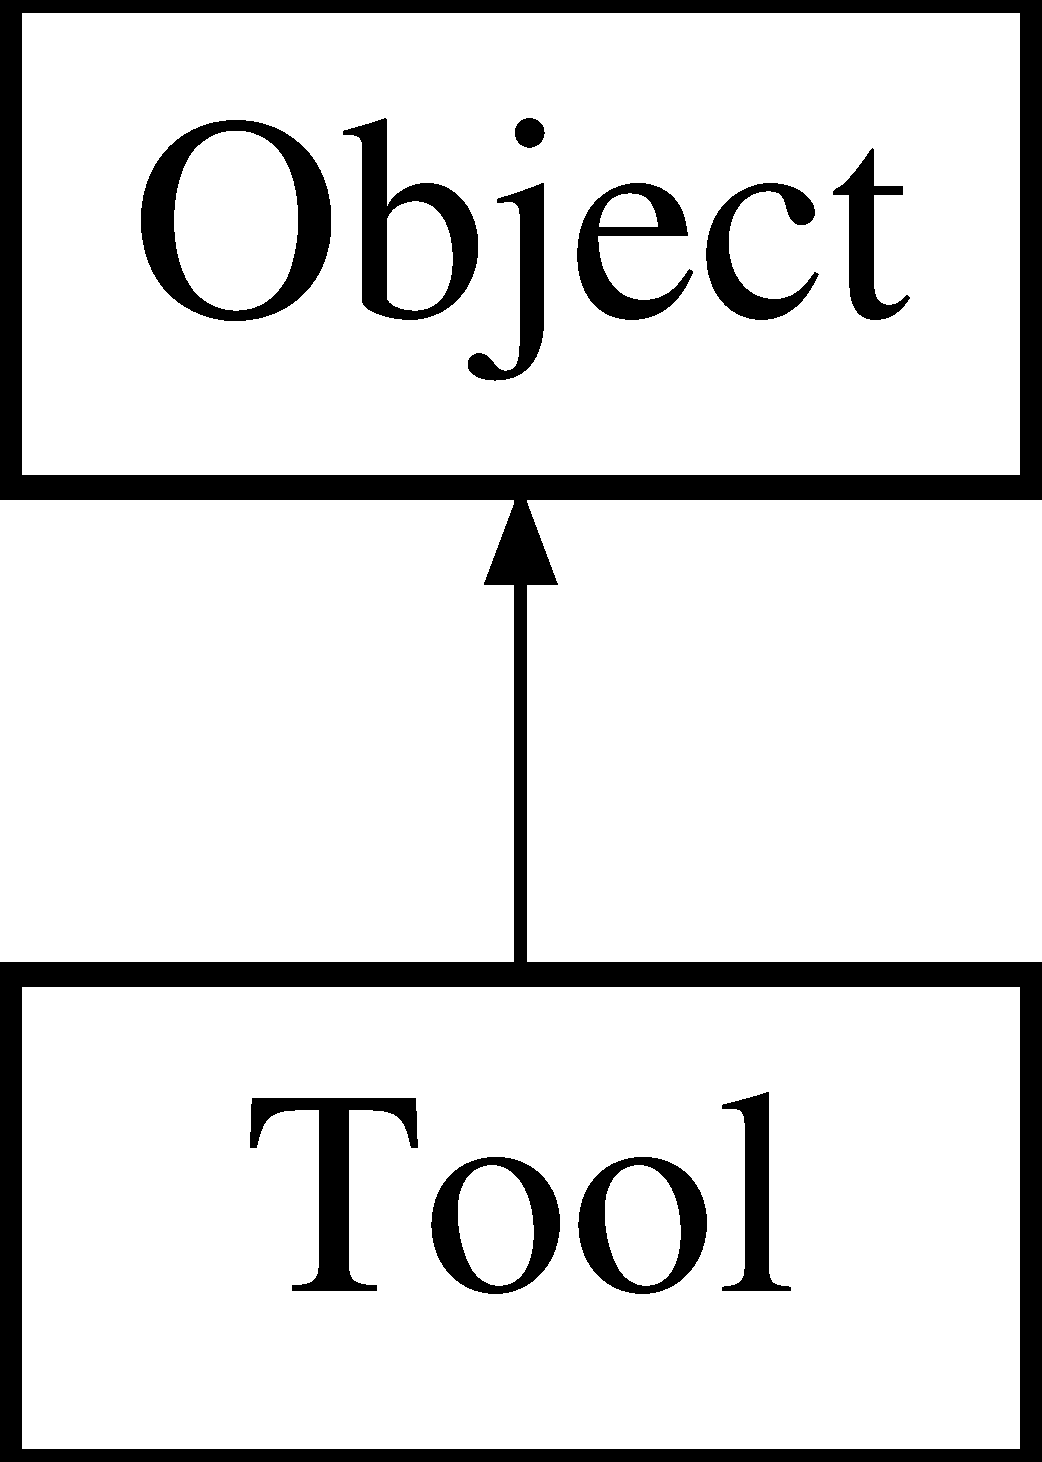
\includegraphics[height=2.000000cm]{classTool}
\end{center}
\end{figure}
\subsection*{Public Member Functions}
\begin{DoxyCompactItemize}
\item 
\hyperlink{classTool_aa21c7e32c4978b4f7d2f908f18fee2e8}{Tool} (\hyperlink{BasicTypes_8h_a38675390df8e0ebbab2867be799b7160}{Tool\-Type} type, \hyperlink{BasicTypes_8h_a8571efa4409be32e28abf3ea74a0dbb1}{Resource\-Type} material, \hyperlink{BasicTypes_8h_a91ad9478d81a7aaf2593e8d9c3d06a14}{uint} max\-\_\-strength=0)
\begin{DoxyCompactList}\small\item\em Constructor. \end{DoxyCompactList}\item 
virtual \hyperlink{classTool_a44634ea099b7a49acf87f50e072ce660}{$\sim$\-Tool} ()
\begin{DoxyCompactList}\small\item\em Destructor. \end{DoxyCompactList}\item 
std\-::vector$<$ \hyperlink{classAction}{Action} $>$ $\ast$ \hyperlink{classTool_a022fd16d7301835eff8324ef8447d90c}{get\-Actions} ()
\begin{DoxyCompactList}\small\item\em Gets actions. \end{DoxyCompactList}\item 
\hyperlink{BasicTypes_8h_a91ad9478d81a7aaf2593e8d9c3d06a14}{uint} \hyperlink{classTool_a5f03c710495f2d1f0714427e0c8a742c}{get\-Strength} () const 
\begin{DoxyCompactList}\small\item\em Gets current tool's strength. \end{DoxyCompactList}\item 
\hyperlink{BasicTypes_8h_a91ad9478d81a7aaf2593e8d9c3d06a14}{uint} \hyperlink{classTool_aba9c408fcfa03c41300d0ba26da25e8f}{get\-Max\-Strength} () const 
\begin{DoxyCompactList}\small\item\em Gets maximum possible tool's strength. \end{DoxyCompactList}\item 
void \hyperlink{classTool_ac8e4a7675142aac8624c18ea6e182cd1}{decrease\-Strength} (\hyperlink{BasicTypes_8h_a91ad9478d81a7aaf2593e8d9c3d06a14}{uint} delta)
\begin{DoxyCompactList}\small\item\em Decreases current tool's strength. \end{DoxyCompactList}\item 
void \hyperlink{classTool_a39a24ab98a0b9acfad17f987fd57272e}{increase\-Strength} (\hyperlink{BasicTypes_8h_a91ad9478d81a7aaf2593e8d9c3d06a14}{uint} delta)
\begin{DoxyCompactList}\small\item\em Increases current tool's strength. \end{DoxyCompactList}\item 
void \hyperlink{classTool_aff5fb696dc98cf8892b4db6350495ca5}{damage} (\hyperlink{BasicTypes_8h_a91ad9478d81a7aaf2593e8d9c3d06a14}{uint} delta)
\begin{DoxyCompactList}\small\item\em Damages tool. \end{DoxyCompactList}\item 
void \hyperlink{classTool_ac7103fa90707cbc29ceb31bc7f941571}{heal} (\hyperlink{BasicTypes_8h_a91ad9478d81a7aaf2593e8d9c3d06a14}{uint} delta)
\begin{DoxyCompactList}\small\item\em ''Heals'' tool. \end{DoxyCompactList}\item 
\hyperlink{BasicTypes_8h_a38675390df8e0ebbab2867be799b7160}{Tool\-Type} \hyperlink{classTool_a29cba502e96018d9db4c2ad9bf364732}{get\-Subtype} () const 
\begin{DoxyCompactList}\small\item\em Gets tool's type. \end{DoxyCompactList}\item 
\hyperlink{BasicTypes_8h_a8571efa4409be32e28abf3ea74a0dbb1}{Resource\-Type} \hyperlink{classTool_a1d1c874a76a20b718ce3b7c344a34944}{get\-Material} () const 
\begin{DoxyCompactList}\small\item\em Gets tool's material. \end{DoxyCompactList}\end{DoxyCompactItemize}
\subsection*{Additional Inherited Members}


\subsection{Detailed Description}
\hyperlink{classTool}{Tool} class. 

Definition at line 15 of file Tool.\-h.



\subsection{Constructor \& Destructor Documentation}
\hypertarget{classTool_aa21c7e32c4978b4f7d2f908f18fee2e8}{\index{Tool@{Tool}!Tool@{Tool}}
\index{Tool@{Tool}!Tool@{Tool}}
\subsubsection[{Tool}]{\setlength{\rightskip}{0pt plus 5cm}Tool\-::\-Tool (
\begin{DoxyParamCaption}
\item[{{\bf Tool\-Type}}]{type, }
\item[{{\bf Resource\-Type}}]{material, }
\item[{{\bf uint}}]{max\-\_\-strength = {\ttfamily 0}}
\end{DoxyParamCaption}
)}}\label{classTool_aa21c7e32c4978b4f7d2f908f18fee2e8}


Constructor. 



Definition at line 15 of file Tool.\-cpp.

\hypertarget{classTool_a44634ea099b7a49acf87f50e072ce660}{\index{Tool@{Tool}!$\sim$\-Tool@{$\sim$\-Tool}}
\index{$\sim$\-Tool@{$\sim$\-Tool}!Tool@{Tool}}
\subsubsection[{$\sim$\-Tool}]{\setlength{\rightskip}{0pt plus 5cm}Tool\-::$\sim$\-Tool (
\begin{DoxyParamCaption}
{}
\end{DoxyParamCaption}
)\hspace{0.3cm}{\ttfamily [virtual]}}}\label{classTool_a44634ea099b7a49acf87f50e072ce660}


Destructor. 



Definition at line 64 of file Tool.\-cpp.



\subsection{Member Function Documentation}
\hypertarget{classTool_aff5fb696dc98cf8892b4db6350495ca5}{\index{Tool@{Tool}!damage@{damage}}
\index{damage@{damage}!Tool@{Tool}}
\subsubsection[{damage}]{\setlength{\rightskip}{0pt plus 5cm}void Tool\-::damage (
\begin{DoxyParamCaption}
\item[{{\bf uint}}]{delta}
\end{DoxyParamCaption}
)\hspace{0.3cm}{\ttfamily [virtual]}}}\label{classTool_aff5fb696dc98cf8892b4db6350495ca5}


Damages tool. 


\begin{DoxyParams}{Parameters}
{\em delta} & amount of damage \\
\hline
\end{DoxyParams}


Implements \hyperlink{classObject_a816838bab5c67fce2cead6cb9122ad47}{Object}.



Definition at line 118 of file Tool.\-cpp.

\hypertarget{classTool_ac8e4a7675142aac8624c18ea6e182cd1}{\index{Tool@{Tool}!decrease\-Strength@{decrease\-Strength}}
\index{decrease\-Strength@{decrease\-Strength}!Tool@{Tool}}
\subsubsection[{decrease\-Strength}]{\setlength{\rightskip}{0pt plus 5cm}void Tool\-::decrease\-Strength (
\begin{DoxyParamCaption}
\item[{{\bf uint}}]{delta}
\end{DoxyParamCaption}
)}}\label{classTool_ac8e4a7675142aac8624c18ea6e182cd1}


Decreases current tool's strength. 


\begin{DoxyParams}{Parameters}
{\em delta} & the value to subtract \\
\hline
\end{DoxyParams}


Definition at line 94 of file Tool.\-cpp.

\hypertarget{classTool_a022fd16d7301835eff8324ef8447d90c}{\index{Tool@{Tool}!get\-Actions@{get\-Actions}}
\index{get\-Actions@{get\-Actions}!Tool@{Tool}}
\subsubsection[{get\-Actions}]{\setlength{\rightskip}{0pt plus 5cm}std\-::vector$<$ {\bf Action} $>$ $\ast$ Tool\-::get\-Actions (
\begin{DoxyParamCaption}
{}
\end{DoxyParamCaption}
)\hspace{0.3cm}{\ttfamily [virtual]}}}\label{classTool_a022fd16d7301835eff8324ef8447d90c}


Gets actions. 

\begin{DoxyReturn}{Returns}
vector with actions. 
\end{DoxyReturn}


Implements \hyperlink{classObject_addf0658ee2f8da579d10a6682dc097d7}{Object}.



Definition at line 72 of file Tool.\-cpp.

\hypertarget{classTool_a1d1c874a76a20b718ce3b7c344a34944}{\index{Tool@{Tool}!get\-Material@{get\-Material}}
\index{get\-Material@{get\-Material}!Tool@{Tool}}
\subsubsection[{get\-Material}]{\setlength{\rightskip}{0pt plus 5cm}{\bf Resource\-Type} Tool\-::get\-Material (
\begin{DoxyParamCaption}
{}
\end{DoxyParamCaption}
) const}}\label{classTool_a1d1c874a76a20b718ce3b7c344a34944}


Gets tool's material. 

\begin{DoxyReturn}{Returns}
tool's material 
\end{DoxyReturn}


Definition at line 137 of file Tool.\-cpp.

\hypertarget{classTool_aba9c408fcfa03c41300d0ba26da25e8f}{\index{Tool@{Tool}!get\-Max\-Strength@{get\-Max\-Strength}}
\index{get\-Max\-Strength@{get\-Max\-Strength}!Tool@{Tool}}
\subsubsection[{get\-Max\-Strength}]{\setlength{\rightskip}{0pt plus 5cm}{\bf uint} Tool\-::get\-Max\-Strength (
\begin{DoxyParamCaption}
{}
\end{DoxyParamCaption}
) const}}\label{classTool_aba9c408fcfa03c41300d0ba26da25e8f}


Gets maximum possible tool's strength. 

\begin{DoxyReturn}{Returns}
the value of maximum strength 
\end{DoxyReturn}


Definition at line 89 of file Tool.\-cpp.

\hypertarget{classTool_a5f03c710495f2d1f0714427e0c8a742c}{\index{Tool@{Tool}!get\-Strength@{get\-Strength}}
\index{get\-Strength@{get\-Strength}!Tool@{Tool}}
\subsubsection[{get\-Strength}]{\setlength{\rightskip}{0pt plus 5cm}{\bf uint} Tool\-::get\-Strength (
\begin{DoxyParamCaption}
{}
\end{DoxyParamCaption}
) const}}\label{classTool_a5f03c710495f2d1f0714427e0c8a742c}


Gets current tool's strength. 

\begin{DoxyReturn}{Returns}
the value of current strength 
\end{DoxyReturn}


Definition at line 84 of file Tool.\-cpp.

\hypertarget{classTool_a29cba502e96018d9db4c2ad9bf364732}{\index{Tool@{Tool}!get\-Subtype@{get\-Subtype}}
\index{get\-Subtype@{get\-Subtype}!Tool@{Tool}}
\subsubsection[{get\-Subtype}]{\setlength{\rightskip}{0pt plus 5cm}{\bf Tool\-Type} Tool\-::get\-Subtype (
\begin{DoxyParamCaption}
{}
\end{DoxyParamCaption}
) const}}\label{classTool_a29cba502e96018d9db4c2ad9bf364732}


Gets tool's type. 

\begin{DoxyReturn}{Returns}
tool's type 
\end{DoxyReturn}


Definition at line 132 of file Tool.\-cpp.

\hypertarget{classTool_ac7103fa90707cbc29ceb31bc7f941571}{\index{Tool@{Tool}!heal@{heal}}
\index{heal@{heal}!Tool@{Tool}}
\subsubsection[{heal}]{\setlength{\rightskip}{0pt plus 5cm}void Tool\-::heal (
\begin{DoxyParamCaption}
\item[{{\bf uint}}]{delta}
\end{DoxyParamCaption}
)\hspace{0.3cm}{\ttfamily [virtual]}}}\label{classTool_ac7103fa90707cbc29ceb31bc7f941571}


''Heals'' tool. 


\begin{DoxyParams}{Parameters}
{\em delta} & amount of healing points \\
\hline
\end{DoxyParams}


Implements \hyperlink{classObject_af7f49cb3f3c3bd9cfdbc42beecbbe5bc}{Object}.



Definition at line 123 of file Tool.\-cpp.

\hypertarget{classTool_a39a24ab98a0b9acfad17f987fd57272e}{\index{Tool@{Tool}!increase\-Strength@{increase\-Strength}}
\index{increase\-Strength@{increase\-Strength}!Tool@{Tool}}
\subsubsection[{increase\-Strength}]{\setlength{\rightskip}{0pt plus 5cm}void Tool\-::increase\-Strength (
\begin{DoxyParamCaption}
\item[{{\bf uint}}]{delta}
\end{DoxyParamCaption}
)}}\label{classTool_a39a24ab98a0b9acfad17f987fd57272e}


Increases current tool's strength. 


\begin{DoxyParams}{Parameters}
{\em delta} & the value to add \\
\hline
\end{DoxyParams}


Definition at line 106 of file Tool.\-cpp.



The documentation for this class was generated from the following files\-:\begin{DoxyCompactItemize}
\item 
model/\-World/\-Object/\-Tool/\hyperlink{Tool_8h}{Tool.\-h}\item 
model/\-World/\-Object/\-Tool/\hyperlink{Tool_8cpp}{Tool.\-cpp}\end{DoxyCompactItemize}

\hypertarget{classView}{\section{View Class Reference}
\label{classView}\index{View@{View}}
}


{\ttfamily \#include $<$View.\-h$>$}

\subsection*{Public Member Functions}
\begin{DoxyCompactItemize}
\item 
\hyperlink{classView_a61e1877684d543b12ebc4ece608e22e4}{View} (\hyperlink{classIWorld}{I\-World} $\ast$w)
\begin{DoxyCompactList}\small\item\em Constructor. \end{DoxyCompactList}\item 
\hyperlink{classView_ad0dc854db9aabbea98a334dec89f785c}{$\sim$\-View} ()
\begin{DoxyCompactList}\small\item\em Destructor. \end{DoxyCompactList}\item 
void \hyperlink{classView_a2e088b57c015d551b27605cab3530187}{redraw} ()
\begin{DoxyCompactList}\small\item\em Redraw currently displayed world. \end{DoxyCompactList}\item 
bool \hyperlink{classView_a2a0fd00361df138bd544174c75031f15}{is\-Exit} ()
\begin{DoxyCompactList}\small\item\em checks conditions to exit the program \end{DoxyCompactList}\end{DoxyCompactItemize}


\subsection{Detailed Description}


Definition at line 18 of file View.\-h.



\subsection{Constructor \& Destructor Documentation}
\hypertarget{classView_a61e1877684d543b12ebc4ece608e22e4}{\index{View@{View}!View@{View}}
\index{View@{View}!View@{View}}
\subsubsection[{View}]{\setlength{\rightskip}{0pt plus 5cm}View\-::\-View (
\begin{DoxyParamCaption}
\item[{{\bf I\-World} $\ast$}]{w}
\end{DoxyParamCaption}
)}}\label{classView_a61e1877684d543b12ebc4ece608e22e4}


Constructor. 


\begin{DoxyParams}{Parameters}
{\em w} & world that will be rendered by this class \\
\hline
\end{DoxyParams}


Definition at line 7 of file View.\-cpp.

\hypertarget{classView_ad0dc854db9aabbea98a334dec89f785c}{\index{View@{View}!$\sim$\-View@{$\sim$\-View}}
\index{$\sim$\-View@{$\sim$\-View}!View@{View}}
\subsubsection[{$\sim$\-View}]{\setlength{\rightskip}{0pt plus 5cm}View\-::$\sim$\-View (
\begin{DoxyParamCaption}
{}
\end{DoxyParamCaption}
)}}\label{classView_ad0dc854db9aabbea98a334dec89f785c}


Destructor. 



Definition at line 21 of file View.\-cpp.



\subsection{Member Function Documentation}
\hypertarget{classView_a2a0fd00361df138bd544174c75031f15}{\index{View@{View}!is\-Exit@{is\-Exit}}
\index{is\-Exit@{is\-Exit}!View@{View}}
\subsubsection[{is\-Exit}]{\setlength{\rightskip}{0pt plus 5cm}bool View\-::is\-Exit (
\begin{DoxyParamCaption}
{}
\end{DoxyParamCaption}
)}}\label{classView_a2a0fd00361df138bd544174c75031f15}


checks conditions to exit the program 

\begin{DoxyReturn}{Returns}
result of exit conditions 
\end{DoxyReturn}


Definition at line 60 of file View.\-cpp.

\hypertarget{classView_a2e088b57c015d551b27605cab3530187}{\index{View@{View}!redraw@{redraw}}
\index{redraw@{redraw}!View@{View}}
\subsubsection[{redraw}]{\setlength{\rightskip}{0pt plus 5cm}void View\-::redraw (
\begin{DoxyParamCaption}
{}
\end{DoxyParamCaption}
)}}\label{classView_a2e088b57c015d551b27605cab3530187}


Redraw currently displayed world. 



Definition at line 27 of file View.\-cpp.



The documentation for this class was generated from the following files\-:\begin{DoxyCompactItemize}
\item 
view/\hyperlink{View_8h}{View.\-h}\item 
view/\hyperlink{View_8cpp}{View.\-cpp}\end{DoxyCompactItemize}

\hypertarget{classViewObject}{\section{View\-Object Class Reference}
\label{classViewObject}\index{View\-Object@{View\-Object}}
}


{\ttfamily \#include $<$View\-Object.\-h$>$}

\subsection*{Public Member Functions}
\begin{DoxyCompactItemize}
\item 
\hyperlink{classViewObject_af0967b283bea1626055db213a2fd8ff7}{View\-Object} (\hyperlink{BasicTypes_8h_a842c5e2e69277690b064bf363c017980}{Object\-Type} newtype, double newx, double newy)
\begin{DoxyCompactList}\small\item\em Constructor. \end{DoxyCompactList}\item 
\hyperlink{classViewObject_af4f968a145747cc2b84fd224ac72122b}{$\sim$\-View\-Object} ()
\begin{DoxyCompactList}\small\item\em Destructor. \end{DoxyCompactList}\item 
void \hyperlink{classViewObject_a6326cc5b3e2151479f8f57149d67bcd8}{set\-Type} (\hyperlink{BasicTypes_8h_a842c5e2e69277690b064bf363c017980}{Object\-Type} new\-\_\-var)
\begin{DoxyCompactList}\small\item\em This variable tells what animation to render. \end{DoxyCompactList}\item 
\hyperlink{BasicTypes_8h_a842c5e2e69277690b064bf363c017980}{Object\-Type} \hyperlink{classViewObject_a4036d3daa7bdd910dc0aa6c6bf5326c7}{get\-Type} ()
\begin{DoxyCompactList}\small\item\em Get the type of current object. \end{DoxyCompactList}\item 
double \hyperlink{classViewObject_a3bb8e2fe8dbd3860d0c3fbda48ad9aab}{get\-X} ()
\begin{DoxyCompactList}\small\item\em Get the x coordinate. \end{DoxyCompactList}\item 
void \hyperlink{classViewObject_a280ef0f29dd3a14d285e816b1798639d}{set\-X} (\hyperlink{BasicTypes_8h_a842c5e2e69277690b064bf363c017980}{Object\-Type} new\-\_\-var)
\begin{DoxyCompactList}\small\item\em Set x coordinate of an object. \end{DoxyCompactList}\item 
double \hyperlink{classViewObject_a4823c2380b8cb092a56ce896a235b7c1}{get\-Y} ()
\begin{DoxyCompactList}\small\item\em Get the y coordinate. \end{DoxyCompactList}\item 
void \hyperlink{classViewObject_af7e0d64500d95544654420876d7f85b8}{set\-Y} (\hyperlink{BasicTypes_8h_a842c5e2e69277690b064bf363c017980}{Object\-Type} new\-\_\-var)
\begin{DoxyCompactList}\small\item\em Set y coordinate of an object. \end{DoxyCompactList}\end{DoxyCompactItemize}


\subsection{Detailed Description}


Definition at line 11 of file View\-Object.\-h.



\subsection{Constructor \& Destructor Documentation}
\hypertarget{classViewObject_af0967b283bea1626055db213a2fd8ff7}{\index{View\-Object@{View\-Object}!View\-Object@{View\-Object}}
\index{View\-Object@{View\-Object}!ViewObject@{View\-Object}}
\subsubsection[{View\-Object}]{\setlength{\rightskip}{0pt plus 5cm}View\-Object\-::\-View\-Object (
\begin{DoxyParamCaption}
\item[{{\bf Object\-Type}}]{newtype, }
\item[{double}]{newx, }
\item[{double}]{newy}
\end{DoxyParamCaption}
)}}\label{classViewObject_af0967b283bea1626055db213a2fd8ff7}


Constructor. 


\begin{DoxyParams}{Parameters}
{\em newtype} & type of the created object \\
\hline
{\em newx} & X coordinate of the created object relative to screen center \\
\hline
{\em newy} & Y coordinate of the created object relative to screen center \\
\hline
\end{DoxyParams}


Definition at line 7 of file View\-Object.\-cpp.

\hypertarget{classViewObject_af4f968a145747cc2b84fd224ac72122b}{\index{View\-Object@{View\-Object}!$\sim$\-View\-Object@{$\sim$\-View\-Object}}
\index{$\sim$\-View\-Object@{$\sim$\-View\-Object}!ViewObject@{View\-Object}}
\subsubsection[{$\sim$\-View\-Object}]{\setlength{\rightskip}{0pt plus 5cm}View\-Object\-::$\sim$\-View\-Object (
\begin{DoxyParamCaption}
{}
\end{DoxyParamCaption}
)}}\label{classViewObject_af4f968a145747cc2b84fd224ac72122b}


Destructor. 



Definition at line 15 of file View\-Object.\-cpp.



\subsection{Member Function Documentation}
\hypertarget{classViewObject_a4036d3daa7bdd910dc0aa6c6bf5326c7}{\index{View\-Object@{View\-Object}!get\-Type@{get\-Type}}
\index{get\-Type@{get\-Type}!ViewObject@{View\-Object}}
\subsubsection[{get\-Type}]{\setlength{\rightskip}{0pt plus 5cm}{\bf Object\-Type} View\-Object\-::get\-Type (
\begin{DoxyParamCaption}
{}
\end{DoxyParamCaption}
)}}\label{classViewObject_a4036d3daa7bdd910dc0aa6c6bf5326c7}


Get the type of current object. 

\begin{DoxyReturn}{Returns}
the value of type 
\end{DoxyReturn}


Definition at line 29 of file View\-Object.\-cpp.

\hypertarget{classViewObject_a3bb8e2fe8dbd3860d0c3fbda48ad9aab}{\index{View\-Object@{View\-Object}!get\-X@{get\-X}}
\index{get\-X@{get\-X}!ViewObject@{View\-Object}}
\subsubsection[{get\-X}]{\setlength{\rightskip}{0pt plus 5cm}double View\-Object\-::get\-X (
\begin{DoxyParamCaption}
{}
\end{DoxyParamCaption}
)}}\label{classViewObject_a3bb8e2fe8dbd3860d0c3fbda48ad9aab}


Get the x coordinate. 

\begin{DoxyReturn}{Returns}
the value of x 
\end{DoxyReturn}


Definition at line 34 of file View\-Object.\-cpp.

\hypertarget{classViewObject_a4823c2380b8cb092a56ce896a235b7c1}{\index{View\-Object@{View\-Object}!get\-Y@{get\-Y}}
\index{get\-Y@{get\-Y}!ViewObject@{View\-Object}}
\subsubsection[{get\-Y}]{\setlength{\rightskip}{0pt plus 5cm}double View\-Object\-::get\-Y (
\begin{DoxyParamCaption}
{}
\end{DoxyParamCaption}
)}}\label{classViewObject_a4823c2380b8cb092a56ce896a235b7c1}


Get the y coordinate. 

\begin{DoxyReturn}{Returns}
the value of y 
\end{DoxyReturn}


Definition at line 39 of file View\-Object.\-cpp.

\hypertarget{classViewObject_a6326cc5b3e2151479f8f57149d67bcd8}{\index{View\-Object@{View\-Object}!set\-Type@{set\-Type}}
\index{set\-Type@{set\-Type}!ViewObject@{View\-Object}}
\subsubsection[{set\-Type}]{\setlength{\rightskip}{0pt plus 5cm}void View\-Object\-::set\-Type (
\begin{DoxyParamCaption}
\item[{{\bf Object\-Type}}]{new\-\_\-var}
\end{DoxyParamCaption}
)}}\label{classViewObject_a6326cc5b3e2151479f8f57149d67bcd8}


This variable tells what animation to render. 

Set the type of current object. 
\begin{DoxyParams}{Parameters}
{\em new\-\_\-var} & the new value of type \\
\hline
\end{DoxyParams}


Definition at line 24 of file View\-Object.\-cpp.

\hypertarget{classViewObject_a280ef0f29dd3a14d285e816b1798639d}{\index{View\-Object@{View\-Object}!set\-X@{set\-X}}
\index{set\-X@{set\-X}!ViewObject@{View\-Object}}
\subsubsection[{set\-X}]{\setlength{\rightskip}{0pt plus 5cm}void View\-Object\-::set\-X (
\begin{DoxyParamCaption}
\item[{{\bf Object\-Type}}]{new\-\_\-var}
\end{DoxyParamCaption}
)}}\label{classViewObject_a280ef0f29dd3a14d285e816b1798639d}


Set x coordinate of an object. 


\begin{DoxyParams}{Parameters}
{\em new\-\_\-var} & the new value of x \\
\hline
\end{DoxyParams}


Definition at line 49 of file View\-Object.\-cpp.

\hypertarget{classViewObject_af7e0d64500d95544654420876d7f85b8}{\index{View\-Object@{View\-Object}!set\-Y@{set\-Y}}
\index{set\-Y@{set\-Y}!ViewObject@{View\-Object}}
\subsubsection[{set\-Y}]{\setlength{\rightskip}{0pt plus 5cm}void View\-Object\-::set\-Y (
\begin{DoxyParamCaption}
\item[{{\bf Object\-Type}}]{new\-\_\-var}
\end{DoxyParamCaption}
)}}\label{classViewObject_af7e0d64500d95544654420876d7f85b8}


Set y coordinate of an object. 


\begin{DoxyParams}{Parameters}
{\em new\-\_\-var} & the new value of y \\
\hline
\end{DoxyParams}


Definition at line 44 of file View\-Object.\-cpp.



The documentation for this class was generated from the following files\-:\begin{DoxyCompactItemize}
\item 
view/\-View\-Object/\hyperlink{ViewObject_8h}{View\-Object.\-h}\item 
view/\-View\-Object/\hyperlink{ViewObject_8cpp}{View\-Object.\-cpp}\end{DoxyCompactItemize}

\hypertarget{classViewWorld}{\section{View\-World Class Reference}
\label{classViewWorld}\index{View\-World@{View\-World}}
}


{\ttfamily \#include $<$View\-World.\-h$>$}

\subsection*{Public Member Functions}
\begin{DoxyCompactItemize}
\item 
\hyperlink{classViewWorld_a010e83eebcfa828f288e4c186ac97284}{View\-World} (\hyperlink{classIWorld}{I\-World} $\ast$w)
\begin{DoxyCompactList}\small\item\em Constructor. \end{DoxyCompactList}\item 
\hyperlink{classViewWorld_abb9df78187bde4033e76a0b54040bf7c}{$\sim$\-View\-World} ()
\begin{DoxyCompactList}\small\item\em Destructor. \end{DoxyCompactList}\item 
void \hyperlink{classViewWorld_aad2482a6e97ebf49c0c2c6be94790ed6}{redraw} ()
\begin{DoxyCompactList}\small\item\em redraw background and all objects in range of the game camera \end{DoxyCompactList}\item 
void \hyperlink{classViewWorld_a7ebce26c23ecfd8440b963bca91bb5bb}{set\-X} (double new\-\_\-var)
\begin{DoxyCompactList}\small\item\em set coordinates of center of the game cam \end{DoxyCompactList}\item 
void \hyperlink{classViewWorld_afde0728835545722c51fcf1c88eba6d0}{set\-Y} (double new\-\_\-var)
\end{DoxyCompactItemize}


\subsection{Detailed Description}


Definition at line 17 of file View\-World.\-h.



\subsection{Constructor \& Destructor Documentation}
\hypertarget{classViewWorld_a010e83eebcfa828f288e4c186ac97284}{\index{View\-World@{View\-World}!View\-World@{View\-World}}
\index{View\-World@{View\-World}!ViewWorld@{View\-World}}
\subsubsection[{View\-World}]{\setlength{\rightskip}{0pt plus 5cm}View\-World\-::\-View\-World (
\begin{DoxyParamCaption}
\item[{{\bf I\-World} $\ast$}]{w}
\end{DoxyParamCaption}
)}}\label{classViewWorld_a010e83eebcfa828f288e4c186ac97284}


Constructor. 


\begin{DoxyParams}{Parameters}
{\em w} & world to render \\
\hline
\end{DoxyParams}


Definition at line 7 of file View\-World.\-cpp.

\hypertarget{classViewWorld_abb9df78187bde4033e76a0b54040bf7c}{\index{View\-World@{View\-World}!$\sim$\-View\-World@{$\sim$\-View\-World}}
\index{$\sim$\-View\-World@{$\sim$\-View\-World}!ViewWorld@{View\-World}}
\subsubsection[{$\sim$\-View\-World}]{\setlength{\rightskip}{0pt plus 5cm}View\-World\-::$\sim$\-View\-World (
\begin{DoxyParamCaption}
{}
\end{DoxyParamCaption}
)}}\label{classViewWorld_abb9df78187bde4033e76a0b54040bf7c}


Destructor. 



Definition at line 26 of file View\-World.\-cpp.



\subsection{Member Function Documentation}
\hypertarget{classViewWorld_aad2482a6e97ebf49c0c2c6be94790ed6}{\index{View\-World@{View\-World}!redraw@{redraw}}
\index{redraw@{redraw}!ViewWorld@{View\-World}}
\subsubsection[{redraw}]{\setlength{\rightskip}{0pt plus 5cm}void View\-World\-::redraw (
\begin{DoxyParamCaption}
{}
\end{DoxyParamCaption}
)}}\label{classViewWorld_aad2482a6e97ebf49c0c2c6be94790ed6}


redraw background and all objects in range of the game camera 



Definition at line 52 of file View\-World.\-cpp.

\hypertarget{classViewWorld_a7ebce26c23ecfd8440b963bca91bb5bb}{\index{View\-World@{View\-World}!set\-X@{set\-X}}
\index{set\-X@{set\-X}!ViewWorld@{View\-World}}
\subsubsection[{set\-X}]{\setlength{\rightskip}{0pt plus 5cm}void View\-World\-::set\-X (
\begin{DoxyParamCaption}
\item[{double}]{new\-\_\-var}
\end{DoxyParamCaption}
)}}\label{classViewWorld_a7ebce26c23ecfd8440b963bca91bb5bb}


set coordinates of center of the game cam 



Definition at line 68 of file View\-World.\-cpp.

\hypertarget{classViewWorld_afde0728835545722c51fcf1c88eba6d0}{\index{View\-World@{View\-World}!set\-Y@{set\-Y}}
\index{set\-Y@{set\-Y}!ViewWorld@{View\-World}}
\subsubsection[{set\-Y}]{\setlength{\rightskip}{0pt plus 5cm}void View\-World\-::set\-Y (
\begin{DoxyParamCaption}
\item[{double}]{new\-\_\-var}
\end{DoxyParamCaption}
)}}\label{classViewWorld_afde0728835545722c51fcf1c88eba6d0}


Definition at line 73 of file View\-World.\-cpp.



The documentation for this class was generated from the following files\-:\begin{DoxyCompactItemize}
\item 
view/\-View\-World/\hyperlink{ViewWorld_8h}{View\-World.\-h}\item 
view/\-View\-World/\hyperlink{ViewWorld_8cpp}{View\-World.\-cpp}\end{DoxyCompactItemize}

\hypertarget{classWeather}{\section{Weather Class Reference}
\label{classWeather}\index{Weather@{Weather}}
}


\hyperlink{classWeather}{Weather} class.  




{\ttfamily \#include $<$Weather.\-h$>$}

Inheritance diagram for Weather\-:\begin{figure}[H]
\begin{center}
\leavevmode
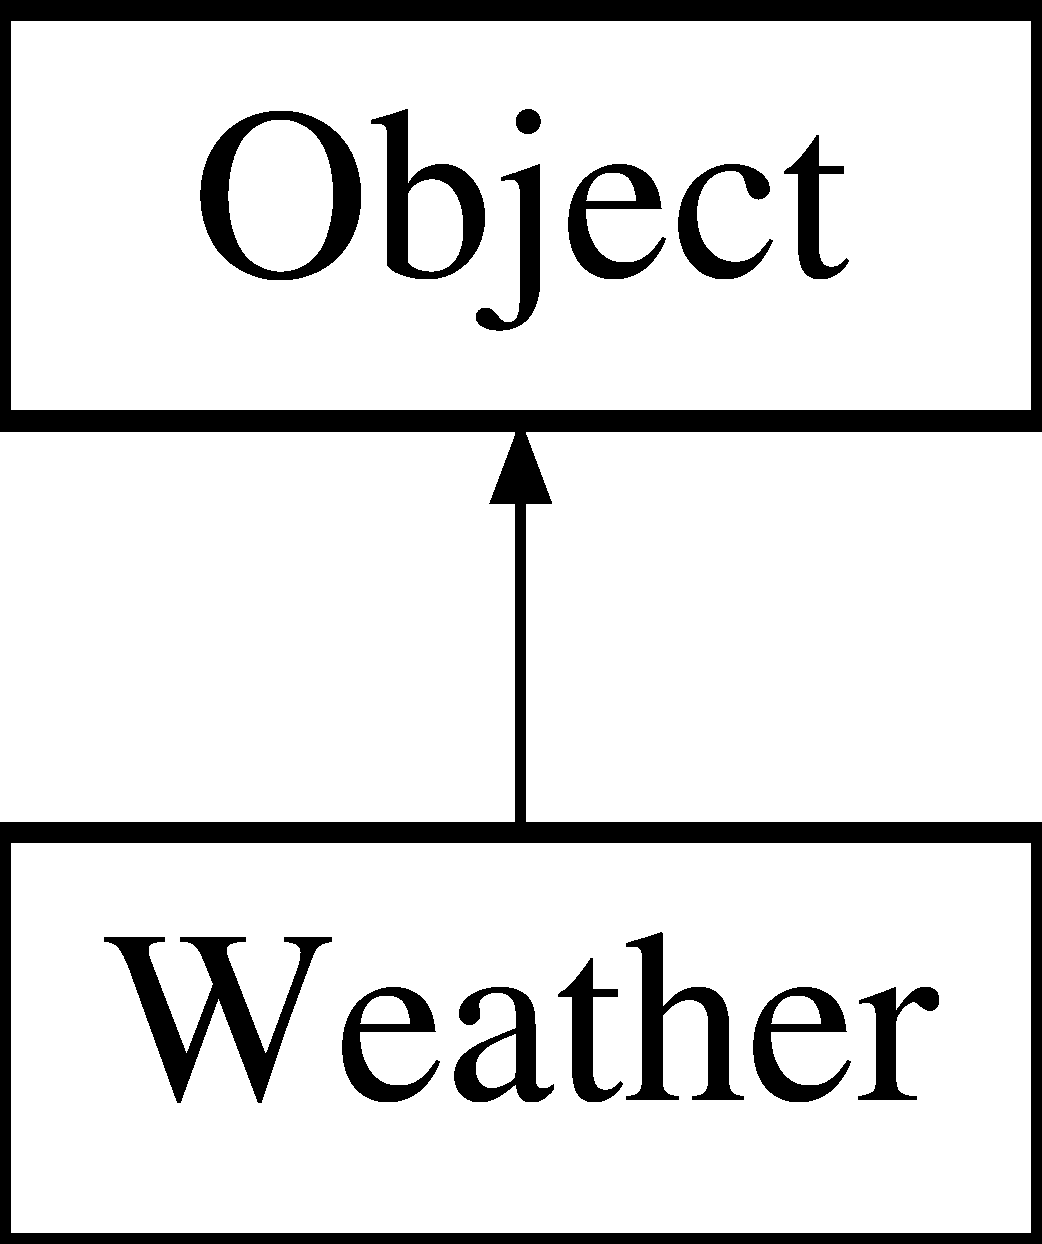
\includegraphics[height=2.000000cm]{classWeather}
\end{center}
\end{figure}
\subsection*{Public Member Functions}
\begin{DoxyCompactItemize}
\item 
\hyperlink{classWeather_aecb2d4cf892c498e09bf9e8a00ae9cbd}{Weather} (\hyperlink{BasicTypes_8h_aae2a79ad426e847c0ddfd77d04ce2516}{Weather\-Type} type, \hyperlink{BasicTypes_8h_a91ad9478d81a7aaf2593e8d9c3d06a14}{uint} living\-\_\-steps=0)
\begin{DoxyCompactList}\small\item\em Constructor. \end{DoxyCompactList}\item 
virtual \hyperlink{classWeather_a6cc4f6ce440531f5c882547dcf40eb22}{$\sim$\-Weather} ()
\begin{DoxyCompactList}\small\item\em Destructor. \end{DoxyCompactList}\item 
std\-::vector$<$ \hyperlink{classAction}{Action} $>$ $\ast$ \hyperlink{classWeather_af6a985a031c55cc9d384fe532bbf69ef}{get\-Actions} ()
\begin{DoxyCompactList}\small\item\em Gets actions. \end{DoxyCompactList}\item 
\hyperlink{BasicTypes_8h_aae2a79ad426e847c0ddfd77d04ce2516}{Weather\-Type} \hyperlink{classWeather_ac2d3f1b253d6616c32a78310b8e05b9a}{get\-Subtype} () const 
\begin{DoxyCompactList}\small\item\em Get the value of subtype. \end{DoxyCompactList}\item 
void \hyperlink{classWeather_a2d2c127d06a55f388a80aedd07b6c2fb}{damage} (\hyperlink{BasicTypes_8h_a91ad9478d81a7aaf2593e8d9c3d06a14}{uint} delta)
\begin{DoxyCompactList}\small\item\em Damages weather (actually does nothing). \end{DoxyCompactList}\item 
void \hyperlink{classWeather_abe32b96dd46b0ce43b3b663a7b1de56c}{heal} (\hyperlink{BasicTypes_8h_a91ad9478d81a7aaf2593e8d9c3d06a14}{uint} delta)
\begin{DoxyCompactList}\small\item\em ''Heals'' weather (actually does nothing). \end{DoxyCompactList}\item 
\hyperlink{classObjectHeap}{Object\-Heap} $\ast$ \hyperlink{classWeather_a2b0841a5845ca5abf437d44c828830dd}{get\-Covered\-Objects} ()
\begin{DoxyCompactList}\small\item\em Gets reference to heap with covered objects. This heap can be modified (in fact, \hyperlink{classController}{Controller} modify it by using \hyperlink{classWeather}{Weather} shape). \end{DoxyCompactList}\item 
\hyperlink{BasicTypes_8h_a91ad9478d81a7aaf2593e8d9c3d06a14}{uint} \hyperlink{classWeather_acfe16f3f5d7e762de9f199a685561d4e}{get\-Living\-Steps} () const 
\begin{DoxyCompactList}\small\item\em Gets amount of living steps. \end{DoxyCompactList}\end{DoxyCompactItemize}
\subsection*{Additional Inherited Members}


\subsection{Detailed Description}
\hyperlink{classWeather}{Weather} class. 

Definition at line 16 of file Weather.\-h.



\subsection{Constructor \& Destructor Documentation}
\hypertarget{classWeather_aecb2d4cf892c498e09bf9e8a00ae9cbd}{\index{Weather@{Weather}!Weather@{Weather}}
\index{Weather@{Weather}!Weather@{Weather}}
\subsubsection[{Weather}]{\setlength{\rightskip}{0pt plus 5cm}Weather\-::\-Weather (
\begin{DoxyParamCaption}
\item[{{\bf Weather\-Type}}]{type, }
\item[{{\bf uint}}]{living\-\_\-steps = {\ttfamily 0}}
\end{DoxyParamCaption}
)}}\label{classWeather_aecb2d4cf892c498e09bf9e8a00ae9cbd}


Constructor. 



Definition at line 15 of file Weather.\-cpp.

\hypertarget{classWeather_a6cc4f6ce440531f5c882547dcf40eb22}{\index{Weather@{Weather}!$\sim$\-Weather@{$\sim$\-Weather}}
\index{$\sim$\-Weather@{$\sim$\-Weather}!Weather@{Weather}}
\subsubsection[{$\sim$\-Weather}]{\setlength{\rightskip}{0pt plus 5cm}Weather\-::$\sim$\-Weather (
\begin{DoxyParamCaption}
{}
\end{DoxyParamCaption}
)\hspace{0.3cm}{\ttfamily [virtual]}}}\label{classWeather_a6cc4f6ce440531f5c882547dcf40eb22}


Destructor. 



Definition at line 33 of file Weather.\-cpp.



\subsection{Member Function Documentation}
\hypertarget{classWeather_a2d2c127d06a55f388a80aedd07b6c2fb}{\index{Weather@{Weather}!damage@{damage}}
\index{damage@{damage}!Weather@{Weather}}
\subsubsection[{damage}]{\setlength{\rightskip}{0pt plus 5cm}void Weather\-::damage (
\begin{DoxyParamCaption}
\item[{{\bf uint}}]{delta}
\end{DoxyParamCaption}
)\hspace{0.3cm}{\ttfamily [inline]}, {\ttfamily [virtual]}}}\label{classWeather_a2d2c127d06a55f388a80aedd07b6c2fb}


Damages weather (actually does nothing). 


\begin{DoxyParams}{Parameters}
{\em delta} & amount of damage \\
\hline
\end{DoxyParams}


Implements \hyperlink{classObject_a816838bab5c67fce2cead6cb9122ad47}{Object}.



Definition at line 61 of file Weather.\-h.

\hypertarget{classWeather_af6a985a031c55cc9d384fe532bbf69ef}{\index{Weather@{Weather}!get\-Actions@{get\-Actions}}
\index{get\-Actions@{get\-Actions}!Weather@{Weather}}
\subsubsection[{get\-Actions}]{\setlength{\rightskip}{0pt plus 5cm}std\-::vector$<$ {\bf Action} $>$ $\ast$ Weather\-::get\-Actions (
\begin{DoxyParamCaption}
{}
\end{DoxyParamCaption}
)\hspace{0.3cm}{\ttfamily [virtual]}}}\label{classWeather_af6a985a031c55cc9d384fe532bbf69ef}


Gets actions. 

\begin{DoxyReturn}{Returns}
vector with actions. 
\end{DoxyReturn}


Implements \hyperlink{classObject_addf0658ee2f8da579d10a6682dc097d7}{Object}.



Definition at line 42 of file Weather.\-cpp.

\hypertarget{classWeather_a2b0841a5845ca5abf437d44c828830dd}{\index{Weather@{Weather}!get\-Covered\-Objects@{get\-Covered\-Objects}}
\index{get\-Covered\-Objects@{get\-Covered\-Objects}!Weather@{Weather}}
\subsubsection[{get\-Covered\-Objects}]{\setlength{\rightskip}{0pt plus 5cm}{\bf Object\-Heap} $\ast$ Weather\-::get\-Covered\-Objects (
\begin{DoxyParamCaption}
{}
\end{DoxyParamCaption}
)}}\label{classWeather_a2b0841a5845ca5abf437d44c828830dd}


Gets reference to heap with covered objects. This heap can be modified (in fact, \hyperlink{classController}{Controller} modify it by using \hyperlink{classWeather}{Weather} shape). 

\begin{DoxyReturn}{Returns}
reference to heap with covered objects 
\end{DoxyReturn}


Definition at line 92 of file Weather.\-cpp.

\hypertarget{classWeather_acfe16f3f5d7e762de9f199a685561d4e}{\index{Weather@{Weather}!get\-Living\-Steps@{get\-Living\-Steps}}
\index{get\-Living\-Steps@{get\-Living\-Steps}!Weather@{Weather}}
\subsubsection[{get\-Living\-Steps}]{\setlength{\rightskip}{0pt plus 5cm}{\bf uint} Weather\-::get\-Living\-Steps (
\begin{DoxyParamCaption}
{}
\end{DoxyParamCaption}
) const}}\label{classWeather_acfe16f3f5d7e762de9f199a685561d4e}


Gets amount of living steps. 

\begin{DoxyReturn}{Returns}
amount of living steps. 
\end{DoxyReturn}


Definition at line 97 of file Weather.\-cpp.

\hypertarget{classWeather_ac2d3f1b253d6616c32a78310b8e05b9a}{\index{Weather@{Weather}!get\-Subtype@{get\-Subtype}}
\index{get\-Subtype@{get\-Subtype}!Weather@{Weather}}
\subsubsection[{get\-Subtype}]{\setlength{\rightskip}{0pt plus 5cm}{\bf Weather\-Type} Weather\-::get\-Subtype (
\begin{DoxyParamCaption}
{}
\end{DoxyParamCaption}
) const}}\label{classWeather_ac2d3f1b253d6616c32a78310b8e05b9a}


Get the value of subtype. 

\begin{DoxyReturn}{Returns}
the value of subtype 
\end{DoxyReturn}


Definition at line 83 of file Weather.\-cpp.

\hypertarget{classWeather_abe32b96dd46b0ce43b3b663a7b1de56c}{\index{Weather@{Weather}!heal@{heal}}
\index{heal@{heal}!Weather@{Weather}}
\subsubsection[{heal}]{\setlength{\rightskip}{0pt plus 5cm}void Weather\-::heal (
\begin{DoxyParamCaption}
\item[{{\bf uint}}]{delta}
\end{DoxyParamCaption}
)\hspace{0.3cm}{\ttfamily [inline]}, {\ttfamily [virtual]}}}\label{classWeather_abe32b96dd46b0ce43b3b663a7b1de56c}


''Heals'' weather (actually does nothing). 


\begin{DoxyParams}{Parameters}
{\em delta} & amount of healing points \\
\hline
\end{DoxyParams}


Implements \hyperlink{classObject_af7f49cb3f3c3bd9cfdbc42beecbbe5bc}{Object}.



Definition at line 67 of file Weather.\-h.



The documentation for this class was generated from the following files\-:\begin{DoxyCompactItemize}
\item 
model/\-World/\-Object/\-Weather/\hyperlink{Weather_8h}{Weather.\-h}\item 
model/\-World/\-Object/\-Weather/\hyperlink{Weather_8cpp}{Weather.\-cpp}\end{DoxyCompactItemize}

\hypertarget{classWorld}{\section{World Class Reference}
\label{classWorld}\index{World@{World}}
}


Class containing methods for primary model interaction.  




{\ttfamily \#include $<$World.\-h$>$}

Inheritance diagram for World\-:\begin{figure}[H]
\begin{center}
\leavevmode
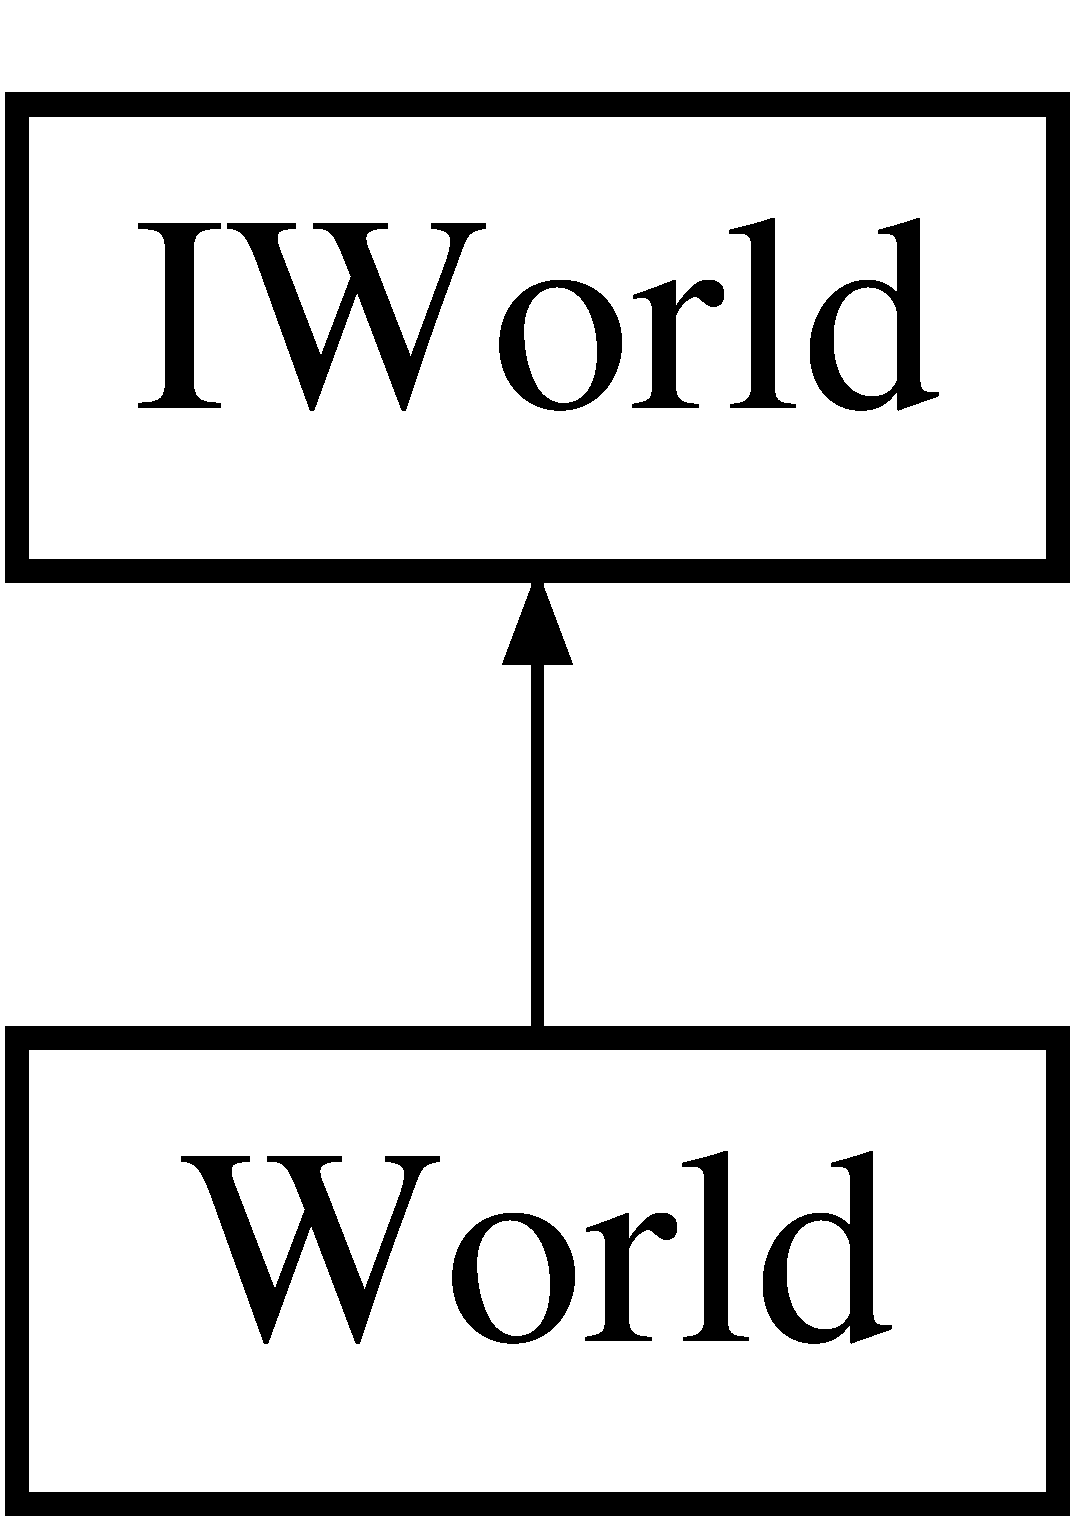
\includegraphics[height=2.000000cm]{classWorld}
\end{center}
\end{figure}
\subsection*{Public Member Functions}
\begin{DoxyCompactItemize}
\item 
virtual \hyperlink{classWorld_a8c73fba541a5817fff65147ba47cd827}{$\sim$\-World} ()
\begin{DoxyCompactList}\small\item\em Destructor. \end{DoxyCompactList}\item 
\hyperlink{classWorld_ac339c606fb3832d11bcf16ad05685f61}{World} (std\-::string filepath)
\begin{DoxyCompactList}\small\item\em Load saved world from file. \end{DoxyCompactList}\item 
\hyperlink{classWorld_aa2eb821136019047477f955fe3d8e7b0}{World} (int rand\-\_\-seed=0, int size=\hyperlink{World_8h_a9771cabfd673a8e350f1f8ce0b8f458f}{D\-E\-F\-A\-U\-L\-T\-\_\-\-S\-I\-Z\-E})
\begin{DoxyCompactList}\small\item\em \hyperlink{classWorld}{World} generation by given seed. \end{DoxyCompactList}\item 
void \hyperlink{classWorld_af56d4516a5cf72c93f3e5bb34cd7d5cd}{save} (std\-::string filepath)
\begin{DoxyCompactList}\small\item\em Save world to file. \end{DoxyCompactList}\item 
void \hyperlink{classWorld_a75e7d1877074f95c25c4696b9932d21f}{set\-Object\-Visibility} (\hyperlink{classObject}{Object} $\ast$obj, bool visibility)
\item 
void \hyperlink{classWorld_a5958579b1313daec5993026df26c7f63}{add\-Object} (bool visibility, \hyperlink{classObject}{Object} $\ast$obj)
\begin{DoxyCompactList}\small\item\em Set the value of visible\-\_\-objs. \end{DoxyCompactList}\item 
double \hyperlink{classWorld_a1c3e886903df2a4fcb8bff59e0dbf115}{get\-Size} ()
\begin{DoxyCompactList}\small\item\em Get \hyperlink{classWorld}{World}'s size. \end{DoxyCompactList}\item 
\hyperlink{classIndexator}{Indexator} $\ast$ \hyperlink{classWorld_ad75ce919ba59eb32d7b9aa4b1ec89ea6}{get\-Indexator} ()
\begin{DoxyCompactList}\small\item\em Get \hyperlink{classWorld}{World}'s indexator. \end{DoxyCompactList}\item 
\hyperlink{classObjectFactory}{Object\-Factory} $\ast$ \hyperlink{classWorld_a25dfb5e9ccd3dd5540ccf6f56937ec28}{get\-Object\-Factory} ()
\begin{DoxyCompactList}\small\item\em Get \hyperlink{classWorld}{World}'s object factory. \end{DoxyCompactList}\item 
\hyperlink{classObjectHeap}{Object\-Heap} $\ast$ \hyperlink{classWorld_ae7d9c8d7590bfa0ed18ed42c05106664}{get\-Visible\-Objects} ()
\begin{DoxyCompactList}\small\item\em Get the value of visible\-\_\-objs. \end{DoxyCompactList}\item 
\hyperlink{classObjectHeap}{Object\-Heap} $\ast$ \hyperlink{classWorld_acdde856cd58e64641405806d08650004}{get\-Hidden\-Objects} ()
\begin{DoxyCompactList}\small\item\em Get the value of hidden\-\_\-objs. \end{DoxyCompactList}\item 
\hyperlink{classObject}{Object} $\ast$$\ast$ \hyperlink{classWorld_a4e16dbeed23237902f74b62f229d7d20}{get\-View\-Objects\-In\-Range} (double x, double y, double radius)
\begin{DoxyCompactList}\small\item\em Get objects in certain radius around (x,y) \end{DoxyCompactList}\item 
\hyperlink{BasicTypes_8h_aae2a79ad426e847c0ddfd77d04ce2516}{Weather\-Type} \hyperlink{classWorld_ab2c8d9f05cfbda5430d6a5e8f7754b85}{get\-Weather\-At\-Point} (double x, double y)
\begin{DoxyCompactList}\small\item\em Get weather state at certain coordinates. \end{DoxyCompactList}\end{DoxyCompactItemize}


\subsection{Detailed Description}
Class containing methods for primary model interaction. 

Definition at line 28 of file World.\-h.



\subsection{Constructor \& Destructor Documentation}
\hypertarget{classWorld_a8c73fba541a5817fff65147ba47cd827}{\index{World@{World}!$\sim$\-World@{$\sim$\-World}}
\index{$\sim$\-World@{$\sim$\-World}!World@{World}}
\subsubsection[{$\sim$\-World}]{\setlength{\rightskip}{0pt plus 5cm}World\-::$\sim$\-World (
\begin{DoxyParamCaption}
{}
\end{DoxyParamCaption}
)\hspace{0.3cm}{\ttfamily [virtual]}}}\label{classWorld_a8c73fba541a5817fff65147ba47cd827}


Destructor. 



Definition at line 16 of file World.\-cpp.

\hypertarget{classWorld_ac339c606fb3832d11bcf16ad05685f61}{\index{World@{World}!World@{World}}
\index{World@{World}!World@{World}}
\subsubsection[{World}]{\setlength{\rightskip}{0pt plus 5cm}World\-::\-World (
\begin{DoxyParamCaption}
\item[{std\-::string}]{filepath}
\end{DoxyParamCaption}
)}}\label{classWorld_ac339c606fb3832d11bcf16ad05685f61}


Load saved world from file. 


\begin{DoxyParams}{Parameters}
{\em filepath} & \\
\hline
\end{DoxyParams}


Definition at line 23 of file World.\-cpp.

\hypertarget{classWorld_aa2eb821136019047477f955fe3d8e7b0}{\index{World@{World}!World@{World}}
\index{World@{World}!World@{World}}
\subsubsection[{World}]{\setlength{\rightskip}{0pt plus 5cm}World\-::\-World (
\begin{DoxyParamCaption}
\item[{int}]{rand\-\_\-seed = {\ttfamily 0}, }
\item[{int}]{size = {\ttfamily {\bf D\-E\-F\-A\-U\-L\-T\-\_\-\-S\-I\-Z\-E}}}
\end{DoxyParamCaption}
)}}\label{classWorld_aa2eb821136019047477f955fe3d8e7b0}


\hyperlink{classWorld}{World} generation by given seed. 


\begin{DoxyParams}{Parameters}
{\em rand\-\_\-seed} & \hyperlink{classWorld}{World} generation by given seed and by specific width/height. \\
\hline
{\em rand\-\_\-seed} & \\
\hline
{\em width} & \\
\hline
{\em height} & \\
\hline
\end{DoxyParams}


Definition at line 29 of file World.\-cpp.



\subsection{Member Function Documentation}
\hypertarget{classWorld_a5958579b1313daec5993026df26c7f63}{\index{World@{World}!add\-Object@{add\-Object}}
\index{add\-Object@{add\-Object}!World@{World}}
\subsubsection[{add\-Object}]{\setlength{\rightskip}{0pt plus 5cm}void World\-::add\-Object (
\begin{DoxyParamCaption}
\item[{bool}]{visibility, }
\item[{{\bf Object} $\ast$}]{obj}
\end{DoxyParamCaption}
)}}\label{classWorld_a5958579b1313daec5993026df26c7f63}


Set the value of visible\-\_\-objs. 


\begin{DoxyParams}{Parameters}
{\em new\-\_\-var} & the new value of visible\-\_\-objs Add an object to \hyperlink{classWorld}{World} \\
\hline
{\em visibility} & \\
\hline
{\em obj} & \\
\hline
\end{DoxyParams}


Definition at line 93 of file World.\-cpp.

\hypertarget{classWorld_acdde856cd58e64641405806d08650004}{\index{World@{World}!get\-Hidden\-Objects@{get\-Hidden\-Objects}}
\index{get\-Hidden\-Objects@{get\-Hidden\-Objects}!World@{World}}
\subsubsection[{get\-Hidden\-Objects}]{\setlength{\rightskip}{0pt plus 5cm}{\bf Object\-Heap} $\ast$ World\-::get\-Hidden\-Objects (
\begin{DoxyParamCaption}
{}
\end{DoxyParamCaption}
)\hspace{0.3cm}{\ttfamily [virtual]}}}\label{classWorld_acdde856cd58e64641405806d08650004}


Get the value of hidden\-\_\-objs. 

\begin{DoxyReturn}{Returns}
the value of hidden\-\_\-objs 
\end{DoxyReturn}


Implements \hyperlink{classIWorld_a1adf8090134ff1742c99b0dacd46b276}{I\-World}.



Definition at line 125 of file World.\-cpp.

\hypertarget{classWorld_ad75ce919ba59eb32d7b9aa4b1ec89ea6}{\index{World@{World}!get\-Indexator@{get\-Indexator}}
\index{get\-Indexator@{get\-Indexator}!World@{World}}
\subsubsection[{get\-Indexator}]{\setlength{\rightskip}{0pt plus 5cm}{\bf Indexator} $\ast$ World\-::get\-Indexator (
\begin{DoxyParamCaption}
{}
\end{DoxyParamCaption}
)\hspace{0.3cm}{\ttfamily [virtual]}}}\label{classWorld_ad75ce919ba59eb32d7b9aa4b1ec89ea6}


Get \hyperlink{classWorld}{World}'s indexator. 

\begin{DoxyReturn}{Returns}
\hyperlink{classWorld}{World}'s indexator 
\end{DoxyReturn}


Implements \hyperlink{classIWorld_a75233893bfd7288b9e7306e08eb2a39d}{I\-World}.



Definition at line 115 of file World.\-cpp.

\hypertarget{classWorld_a25dfb5e9ccd3dd5540ccf6f56937ec28}{\index{World@{World}!get\-Object\-Factory@{get\-Object\-Factory}}
\index{get\-Object\-Factory@{get\-Object\-Factory}!World@{World}}
\subsubsection[{get\-Object\-Factory}]{\setlength{\rightskip}{0pt plus 5cm}{\bf Object\-Factory} $\ast$ World\-::get\-Object\-Factory (
\begin{DoxyParamCaption}
{}
\end{DoxyParamCaption}
)\hspace{0.3cm}{\ttfamily [virtual]}}}\label{classWorld_a25dfb5e9ccd3dd5540ccf6f56937ec28}


Get \hyperlink{classWorld}{World}'s object factory. 

\begin{DoxyReturn}{Returns}
\hyperlink{classWorld}{World}'s object factory 
\end{DoxyReturn}


Implements \hyperlink{classIWorld_a8deb54efc20b8b1d4b966fe5128c9c2b}{I\-World}.



Definition at line 105 of file World.\-cpp.

\hypertarget{classWorld_a1c3e886903df2a4fcb8bff59e0dbf115}{\index{World@{World}!get\-Size@{get\-Size}}
\index{get\-Size@{get\-Size}!World@{World}}
\subsubsection[{get\-Size}]{\setlength{\rightskip}{0pt plus 5cm}double World\-::get\-Size (
\begin{DoxyParamCaption}
{}
\end{DoxyParamCaption}
)\hspace{0.3cm}{\ttfamily [virtual]}}}\label{classWorld_a1c3e886903df2a4fcb8bff59e0dbf115}


Get \hyperlink{classWorld}{World}'s size. 

\begin{DoxyReturn}{Returns}
\hyperlink{classWorld}{World}'s size 
\end{DoxyReturn}


Implements \hyperlink{classIWorld_a3791b170cd91f6d1a71ef958f19d2ac9}{I\-World}.



Definition at line 110 of file World.\-cpp.

\hypertarget{classWorld_a4e16dbeed23237902f74b62f229d7d20}{\index{World@{World}!get\-View\-Objects\-In\-Range@{get\-View\-Objects\-In\-Range}}
\index{get\-View\-Objects\-In\-Range@{get\-View\-Objects\-In\-Range}!World@{World}}
\subsubsection[{get\-View\-Objects\-In\-Range}]{\setlength{\rightskip}{0pt plus 5cm}{\bf Object} $\ast$$\ast$ World\-::get\-View\-Objects\-In\-Range (
\begin{DoxyParamCaption}
\item[{double}]{x, }
\item[{double}]{y, }
\item[{double}]{radius}
\end{DoxyParamCaption}
)\hspace{0.3cm}{\ttfamily [virtual]}}}\label{classWorld_a4e16dbeed23237902f74b62f229d7d20}


Get objects in certain radius around (x,y) 


\begin{DoxyParams}{Parameters}
{\em x} & x coordinate of the range center \\
\hline
{\em y} & y coordinate of the range center \\
\hline
{\em radius} & range from which objects are returned \\
\hline
\end{DoxyParams}
\begin{DoxyReturn}{Returns}
Pointer to \hyperlink{classObjectHeap}{Object\-Heap} of objects in radius around (x,y) Get objects visible in certain radius around a certain point. 
\end{DoxyReturn}

\begin{DoxyParams}{Parameters}
{\em x} & x coordinate of screen center \\
\hline
{\em y} & y coordinate of screen center \\
\hline
{\em radius} & maximal distance from screen center at which object is visible \\
\hline
{\em size} & number of \hyperlink{classViewObject}{View\-Object} instances created \\
\hline
\end{DoxyParams}
\begin{DoxyReturn}{Returns}
array of \hyperlink{classViewObject}{View\-Object}. Coordinates are relative to (x, y) provided array is return null-\/terminated 
\end{DoxyReturn}


Implements \hyperlink{classIWorld_a7c94c8a5db44f1ae707f35e7c4fd3aef}{I\-World}.



Definition at line 142 of file World.\-cpp.

\hypertarget{classWorld_ae7d9c8d7590bfa0ed18ed42c05106664}{\index{World@{World}!get\-Visible\-Objects@{get\-Visible\-Objects}}
\index{get\-Visible\-Objects@{get\-Visible\-Objects}!World@{World}}
\subsubsection[{get\-Visible\-Objects}]{\setlength{\rightskip}{0pt plus 5cm}{\bf Object\-Heap} $\ast$ World\-::get\-Visible\-Objects (
\begin{DoxyParamCaption}
{}
\end{DoxyParamCaption}
)\hspace{0.3cm}{\ttfamily [virtual]}}}\label{classWorld_ae7d9c8d7590bfa0ed18ed42c05106664}


Get the value of visible\-\_\-objs. 

\begin{DoxyReturn}{Returns}
the value of visible\-\_\-objs 
\end{DoxyReturn}


Implements \hyperlink{classIWorld_aae71f283d70ad9f267d6731683e6ab7e}{I\-World}.



Definition at line 120 of file World.\-cpp.

\hypertarget{classWorld_ab2c8d9f05cfbda5430d6a5e8f7754b85}{\index{World@{World}!get\-Weather\-At\-Point@{get\-Weather\-At\-Point}}
\index{get\-Weather\-At\-Point@{get\-Weather\-At\-Point}!World@{World}}
\subsubsection[{get\-Weather\-At\-Point}]{\setlength{\rightskip}{0pt plus 5cm}{\bf Weather\-Type} World\-::get\-Weather\-At\-Point (
\begin{DoxyParamCaption}
\item[{double}]{x, }
\item[{double}]{y}
\end{DoxyParamCaption}
)\hspace{0.3cm}{\ttfamily [virtual]}}}\label{classWorld_ab2c8d9f05cfbda5430d6a5e8f7754b85}


Get weather state at certain coordinates. 


\begin{DoxyParams}{Parameters}
{\em x} & x coordinate of screen center \\
\hline
{\em y} & y coordinate of screen center \\
\hline
\end{DoxyParams}
\begin{DoxyReturn}{Returns}
View\-Weather -\/ enum indicating weather at specified location 
\end{DoxyReturn}


Implements \hyperlink{classIWorld_ac3c29f9aba4066efbe3bbfce51030ad5}{I\-World}.



Definition at line 169 of file World.\-cpp.

\hypertarget{classWorld_af56d4516a5cf72c93f3e5bb34cd7d5cd}{\index{World@{World}!save@{save}}
\index{save@{save}!World@{World}}
\subsubsection[{save}]{\setlength{\rightskip}{0pt plus 5cm}void World\-::save (
\begin{DoxyParamCaption}
\item[{std\-::string}]{filepath}
\end{DoxyParamCaption}
)}}\label{classWorld_af56d4516a5cf72c93f3e5bb34cd7d5cd}


Save world to file. 


\begin{DoxyParams}{Parameters}
{\em filepath} & \\
\hline
\end{DoxyParams}


Definition at line 79 of file World.\-cpp.

\hypertarget{classWorld_a75e7d1877074f95c25c4696b9932d21f}{\index{World@{World}!set\-Object\-Visibility@{set\-Object\-Visibility}}
\index{set\-Object\-Visibility@{set\-Object\-Visibility}!World@{World}}
\subsubsection[{set\-Object\-Visibility}]{\setlength{\rightskip}{0pt plus 5cm}void World\-::set\-Object\-Visibility (
\begin{DoxyParamCaption}
\item[{{\bf Object} $\ast$}]{obj, }
\item[{bool}]{visibility}
\end{DoxyParamCaption}
)}}\label{classWorld_a75e7d1877074f95c25c4696b9932d21f}


Definition at line 74 of file World.\-cpp.



The documentation for this class was generated from the following files\-:\begin{DoxyCompactItemize}
\item 
model/\-World/\hyperlink{World_8h}{World.\-h}\item 
model/\-World/\hyperlink{World_8cpp}{World.\-cpp}\end{DoxyCompactItemize}

\chapter{File Documentation}
\hypertarget{Controller_8cpp}{\section{control/\-Controller/\-Controller.cpp File Reference}
\label{Controller_8cpp}\index{control/\-Controller/\-Controller.\-cpp@{control/\-Controller/\-Controller.\-cpp}}
}
{\ttfamily \#include \char`\"{}../\-Performer/\-Movement\-Performer/\-Movement\-Performer.\-h\char`\"{}}\\*
{\ttfamily \#include \char`\"{}../\-Performer/\-Creation\-Performer/\-Creation\-Performer.\-h\char`\"{}}\\*
{\ttfamily \#include \char`\"{}../\-Performer/\-Harm\-Performer/\-Harm\-Performer.\-h\char`\"{}}\\*
{\ttfamily \#include \char`\"{}../\-Performer/\-Repairing\-Performer/\-Repairing\-Performer.\-h\char`\"{}}\\*
{\ttfamily \#include \char`\"{}../\-Performer/\-Mining\-Performer/\-Mining\-Performer.\-h\char`\"{}}\\*
{\ttfamily \#include \char`\"{}../\-Performer/\-Dropping\-Performer/\-Dropping\-Performer.\-h\char`\"{}}\\*
{\ttfamily \#include \char`\"{}../\-Performer/\-Pickup\-Master/\-Pickup\-Master.\-h\char`\"{}}\\*
{\ttfamily \#include \char`\"{}Controller.\-h\char`\"{}}\\*

\hypertarget{Controller_8h}{\section{control/\-Controller/\-Controller.h File Reference}
\label{Controller_8h}\index{control/\-Controller/\-Controller.\-h@{control/\-Controller/\-Controller.\-h}}
}
{\ttfamily \#include $<$vector$>$}\\*
{\ttfamily \#include \char`\"{}../../model/\-World/\-World.\-h\char`\"{}}\\*
{\ttfamily \#include \char`\"{}../\-Performer/\-Performer.\-h\char`\"{}}\\*
\subsection*{Classes}
\begin{DoxyCompactItemize}
\item 
class \hyperlink{classController}{Controller}
\begin{DoxyCompactList}\small\item\em Class controls the world! \end{DoxyCompactList}\end{DoxyCompactItemize}

\hypertarget{CreationPerformer_8cpp}{\section{control/\-Performer/\-Creation\-Performer/\-Creation\-Performer.cpp File Reference}
\label{CreationPerformer_8cpp}\index{control/\-Performer/\-Creation\-Performer/\-Creation\-Performer.\-cpp@{control/\-Performer/\-Creation\-Performer/\-Creation\-Performer.\-cpp}}
}
{\ttfamily \#include \char`\"{}Creation\-Performer.\-h\char`\"{}}\\*
{\ttfamily \#include \char`\"{}../../../model/\-Basic\-Types.\-h\char`\"{}}\\*
{\ttfamily \#include \char`\"{}../../../model/\-Basic\-Defines.\-h\char`\"{}}\\*
{\ttfamily \#include \char`\"{}../../../model/\-World/\-Object\-Factory/\-Object\-Factory.\-h\char`\"{}}\\*
{\ttfamily \#include \char`\"{}../../../model/\-World/\-Object/\-Creatures/\-Creature.\-h\char`\"{}}\\*

\hypertarget{CreationPerformer_8h}{\section{control/\-Performer/\-Creation\-Performer/\-Creation\-Performer.h File Reference}
\label{CreationPerformer_8h}\index{control/\-Performer/\-Creation\-Performer/\-Creation\-Performer.\-h@{control/\-Performer/\-Creation\-Performer/\-Creation\-Performer.\-h}}
}
{\ttfamily \#include \char`\"{}../../../model/\-World/\-World.\-h\char`\"{}}\\*
{\ttfamily \#include \char`\"{}../\-Performer.\-h\char`\"{}}\\*
{\ttfamily \#include \char`\"{}../../../model/\-World/\-Indexator/\-Indexator.\-h\char`\"{}}\\*
\subsection*{Classes}
\begin{DoxyCompactItemize}
\item 
class \hyperlink{classCreationPerformer}{Creation\-Performer}
\begin{DoxyCompactList}\small\item\em Performs a creation if it is possible. \end{DoxyCompactList}\end{DoxyCompactItemize}

\hypertarget{DroppingPerformer_8cpp}{\section{control/\-Performer/\-Dropping\-Performer/\-Dropping\-Performer.cpp File Reference}
\label{DroppingPerformer_8cpp}\index{control/\-Performer/\-Dropping\-Performer/\-Dropping\-Performer.\-cpp@{control/\-Performer/\-Dropping\-Performer/\-Dropping\-Performer.\-cpp}}
}
{\ttfamily \#include \char`\"{}Dropping\-Performer.\-h\char`\"{}}\\*
{\ttfamily \#include \char`\"{}../../../model/\-World/\-Object/\-Creatures/\-Creature.\-h\char`\"{}}\\*
{\ttfamily \#include $<$string$>$}\\*
{\ttfamily \#include $<$cmath$>$}\\*
\subsection*{Macros}
\begin{DoxyCompactItemize}
\item 
\#define \hyperlink{DroppingPerformer_8cpp_a8c1f6db13c55c6472864e3ad214bd346}{C\-R\-E\-A\-T\-\_\-\-S\-P\-E\-E\-D\-\_\-\-F\-A\-S\-T\-\_\-\-V\-A\-L\-U\-E}~10
\item 
\#define \hyperlink{DroppingPerformer_8cpp_accf4fc5c9f279394d37aa8c9becd3ef6}{C\-R\-E\-A\-T\-\_\-\-S\-P\-E\-E\-D\-\_\-\-S\-L\-O\-W\-\_\-\-V\-A\-L\-U\-E}~5
\end{DoxyCompactItemize}


\subsection{Macro Definition Documentation}
\hypertarget{DroppingPerformer_8cpp_a8c1f6db13c55c6472864e3ad214bd346}{\index{Dropping\-Performer.\-cpp@{Dropping\-Performer.\-cpp}!C\-R\-E\-A\-T\-\_\-\-S\-P\-E\-E\-D\-\_\-\-F\-A\-S\-T\-\_\-\-V\-A\-L\-U\-E@{C\-R\-E\-A\-T\-\_\-\-S\-P\-E\-E\-D\-\_\-\-F\-A\-S\-T\-\_\-\-V\-A\-L\-U\-E}}
\index{C\-R\-E\-A\-T\-\_\-\-S\-P\-E\-E\-D\-\_\-\-F\-A\-S\-T\-\_\-\-V\-A\-L\-U\-E@{C\-R\-E\-A\-T\-\_\-\-S\-P\-E\-E\-D\-\_\-\-F\-A\-S\-T\-\_\-\-V\-A\-L\-U\-E}!DroppingPerformer.cpp@{Dropping\-Performer.\-cpp}}
\subsubsection[{C\-R\-E\-A\-T\-\_\-\-S\-P\-E\-E\-D\-\_\-\-F\-A\-S\-T\-\_\-\-V\-A\-L\-U\-E}]{\setlength{\rightskip}{0pt plus 5cm}\#define C\-R\-E\-A\-T\-\_\-\-S\-P\-E\-E\-D\-\_\-\-F\-A\-S\-T\-\_\-\-V\-A\-L\-U\-E~10}}\label{DroppingPerformer_8cpp_a8c1f6db13c55c6472864e3ad214bd346}


Definition at line 15 of file Dropping\-Performer.\-cpp.

\hypertarget{DroppingPerformer_8cpp_accf4fc5c9f279394d37aa8c9becd3ef6}{\index{Dropping\-Performer.\-cpp@{Dropping\-Performer.\-cpp}!C\-R\-E\-A\-T\-\_\-\-S\-P\-E\-E\-D\-\_\-\-S\-L\-O\-W\-\_\-\-V\-A\-L\-U\-E@{C\-R\-E\-A\-T\-\_\-\-S\-P\-E\-E\-D\-\_\-\-S\-L\-O\-W\-\_\-\-V\-A\-L\-U\-E}}
\index{C\-R\-E\-A\-T\-\_\-\-S\-P\-E\-E\-D\-\_\-\-S\-L\-O\-W\-\_\-\-V\-A\-L\-U\-E@{C\-R\-E\-A\-T\-\_\-\-S\-P\-E\-E\-D\-\_\-\-S\-L\-O\-W\-\_\-\-V\-A\-L\-U\-E}!DroppingPerformer.cpp@{Dropping\-Performer.\-cpp}}
\subsubsection[{C\-R\-E\-A\-T\-\_\-\-S\-P\-E\-E\-D\-\_\-\-S\-L\-O\-W\-\_\-\-V\-A\-L\-U\-E}]{\setlength{\rightskip}{0pt plus 5cm}\#define C\-R\-E\-A\-T\-\_\-\-S\-P\-E\-E\-D\-\_\-\-S\-L\-O\-W\-\_\-\-V\-A\-L\-U\-E~5}}\label{DroppingPerformer_8cpp_accf4fc5c9f279394d37aa8c9becd3ef6}


Definition at line 19 of file Dropping\-Performer.\-cpp.


\hypertarget{DroppingPerformer_8h}{\section{control/\-Performer/\-Dropping\-Performer/\-Dropping\-Performer.h File Reference}
\label{DroppingPerformer_8h}\index{control/\-Performer/\-Dropping\-Performer/\-Dropping\-Performer.\-h@{control/\-Performer/\-Dropping\-Performer/\-Dropping\-Performer.\-h}}
}
{\ttfamily \#include \char`\"{}../\-Performer.\-h\char`\"{}}\\*
{\ttfamily \#include \char`\"{}../../../model/\-World/\-World.\-h\char`\"{}}\\*
\subsection*{Classes}
\begin{DoxyCompactItemize}
\item 
class \hyperlink{classDroppingPerformer}{Dropping\-Performer}
\begin{DoxyCompactList}\small\item\em Performs a drop if possible. \end{DoxyCompactList}\end{DoxyCompactItemize}

\hypertarget{HarmPerformer_8cpp}{\section{control/\-Performer/\-Harm\-Performer/\-Harm\-Performer.cpp File Reference}
\label{HarmPerformer_8cpp}\index{control/\-Performer/\-Harm\-Performer/\-Harm\-Performer.\-cpp@{control/\-Performer/\-Harm\-Performer/\-Harm\-Performer.\-cpp}}
}
{\ttfamily \#include \char`\"{}Harm\-Performer.\-h\char`\"{}}\\*
{\ttfamily \#include \char`\"{}../../../model/\-World/\-Object/\-Object.\-h\char`\"{}}\\*
{\ttfamily \#include \char`\"{}../../../model/\-Basic\-Funcs.\-h\char`\"{}}\\*
{\ttfamily \#include $<$vector$>$}\\*

\hypertarget{HarmPerformer_8h}{\section{control/\-Performer/\-Harm\-Performer/\-Harm\-Performer.h File Reference}
\label{HarmPerformer_8h}\index{control/\-Performer/\-Harm\-Performer/\-Harm\-Performer.\-h@{control/\-Performer/\-Harm\-Performer/\-Harm\-Performer.\-h}}
}
{\ttfamily \#include \char`\"{}../\-Performer.\-h\char`\"{}}\\*
{\ttfamily \#include \char`\"{}../../../model/\-World/\-Indexator/\-Indexator.\-h\char`\"{}}\\*
\subsection*{Classes}
\begin{DoxyCompactItemize}
\item 
class \hyperlink{classHarmPerformer}{Harm\-Performer}
\begin{DoxyCompactList}\small\item\em Performs a harm if it is possible. \end{DoxyCompactList}\end{DoxyCompactItemize}

\hypertarget{MiningPerformer_8cpp}{\section{control/\-Performer/\-Mining\-Performer/\-Mining\-Performer.cpp File Reference}
\label{MiningPerformer_8cpp}\index{control/\-Performer/\-Mining\-Performer/\-Mining\-Performer.\-cpp@{control/\-Performer/\-Mining\-Performer/\-Mining\-Performer.\-cpp}}
}
{\ttfamily \#include \char`\"{}Mining\-Performer.\-h\char`\"{}}\\*

\hypertarget{MiningPerformer_8h}{\section{control/\-Performer/\-Mining\-Performer/\-Mining\-Performer.h File Reference}
\label{MiningPerformer_8h}\index{control/\-Performer/\-Mining\-Performer/\-Mining\-Performer.\-h@{control/\-Performer/\-Mining\-Performer/\-Mining\-Performer.\-h}}
}
{\ttfamily \#include \char`\"{}../\-Performer.\-h\char`\"{}}\\*
{\ttfamily \#include \char`\"{}../../../model/\-World/\-Indexator/\-Indexator.\-h\char`\"{}}\\*
{\ttfamily \#include \char`\"{}../../../model/\-World/\-Object/\-Resource/\-Resource.\-h\char`\"{}}\\*
{\ttfamily \#include \char`\"{}../../../model/\-World/\-Object/\-Tool/\-Tool.\-h\char`\"{}}\\*
\subsection*{Classes}
\begin{DoxyCompactItemize}
\item 
class \hyperlink{classMiningPerformer}{Mining\-Performer}
\begin{DoxyCompactList}\small\item\em Performs a mining if it is possible. \end{DoxyCompactList}\end{DoxyCompactItemize}

\hypertarget{MovementPerformer_8cpp}{\section{control/\-Performer/\-Movement\-Performer/\-Movement\-Performer.cpp File Reference}
\label{MovementPerformer_8cpp}\index{control/\-Performer/\-Movement\-Performer/\-Movement\-Performer.\-cpp@{control/\-Performer/\-Movement\-Performer/\-Movement\-Performer.\-cpp}}
}
{\ttfamily \#include \char`\"{}Movement\-Performer.\-h\char`\"{}}\\*
{\ttfamily \#include $<$string$>$}\\*
{\ttfamily \#include $<$cmath$>$}\\*
\subsection*{Macros}
\begin{DoxyCompactItemize}
\item 
\#define \hyperlink{MovementPerformer_8cpp_a8c1f6db13c55c6472864e3ad214bd346}{C\-R\-E\-A\-T\-\_\-\-S\-P\-E\-E\-D\-\_\-\-F\-A\-S\-T\-\_\-\-V\-A\-L\-U\-E}~10
\item 
\#define \hyperlink{MovementPerformer_8cpp_accf4fc5c9f279394d37aa8c9becd3ef6}{C\-R\-E\-A\-T\-\_\-\-S\-P\-E\-E\-D\-\_\-\-S\-L\-O\-W\-\_\-\-V\-A\-L\-U\-E}~5
\end{DoxyCompactItemize}


\subsection{Macro Definition Documentation}
\hypertarget{MovementPerformer_8cpp_a8c1f6db13c55c6472864e3ad214bd346}{\index{Movement\-Performer.\-cpp@{Movement\-Performer.\-cpp}!C\-R\-E\-A\-T\-\_\-\-S\-P\-E\-E\-D\-\_\-\-F\-A\-S\-T\-\_\-\-V\-A\-L\-U\-E@{C\-R\-E\-A\-T\-\_\-\-S\-P\-E\-E\-D\-\_\-\-F\-A\-S\-T\-\_\-\-V\-A\-L\-U\-E}}
\index{C\-R\-E\-A\-T\-\_\-\-S\-P\-E\-E\-D\-\_\-\-F\-A\-S\-T\-\_\-\-V\-A\-L\-U\-E@{C\-R\-E\-A\-T\-\_\-\-S\-P\-E\-E\-D\-\_\-\-F\-A\-S\-T\-\_\-\-V\-A\-L\-U\-E}!MovementPerformer.cpp@{Movement\-Performer.\-cpp}}
\subsubsection[{C\-R\-E\-A\-T\-\_\-\-S\-P\-E\-E\-D\-\_\-\-F\-A\-S\-T\-\_\-\-V\-A\-L\-U\-E}]{\setlength{\rightskip}{0pt plus 5cm}\#define C\-R\-E\-A\-T\-\_\-\-S\-P\-E\-E\-D\-\_\-\-F\-A\-S\-T\-\_\-\-V\-A\-L\-U\-E~10}}\label{MovementPerformer_8cpp_a8c1f6db13c55c6472864e3ad214bd346}


Definition at line 14 of file Movement\-Performer.\-cpp.

\hypertarget{MovementPerformer_8cpp_accf4fc5c9f279394d37aa8c9becd3ef6}{\index{Movement\-Performer.\-cpp@{Movement\-Performer.\-cpp}!C\-R\-E\-A\-T\-\_\-\-S\-P\-E\-E\-D\-\_\-\-S\-L\-O\-W\-\_\-\-V\-A\-L\-U\-E@{C\-R\-E\-A\-T\-\_\-\-S\-P\-E\-E\-D\-\_\-\-S\-L\-O\-W\-\_\-\-V\-A\-L\-U\-E}}
\index{C\-R\-E\-A\-T\-\_\-\-S\-P\-E\-E\-D\-\_\-\-S\-L\-O\-W\-\_\-\-V\-A\-L\-U\-E@{C\-R\-E\-A\-T\-\_\-\-S\-P\-E\-E\-D\-\_\-\-S\-L\-O\-W\-\_\-\-V\-A\-L\-U\-E}!MovementPerformer.cpp@{Movement\-Performer.\-cpp}}
\subsubsection[{C\-R\-E\-A\-T\-\_\-\-S\-P\-E\-E\-D\-\_\-\-S\-L\-O\-W\-\_\-\-V\-A\-L\-U\-E}]{\setlength{\rightskip}{0pt plus 5cm}\#define C\-R\-E\-A\-T\-\_\-\-S\-P\-E\-E\-D\-\_\-\-S\-L\-O\-W\-\_\-\-V\-A\-L\-U\-E~5}}\label{MovementPerformer_8cpp_accf4fc5c9f279394d37aa8c9becd3ef6}


Definition at line 18 of file Movement\-Performer.\-cpp.


\hypertarget{MovementPerformer_8h}{\section{control/\-Performer/\-Movement\-Performer/\-Movement\-Performer.h File Reference}
\label{MovementPerformer_8h}\index{control/\-Performer/\-Movement\-Performer/\-Movement\-Performer.\-h@{control/\-Performer/\-Movement\-Performer/\-Movement\-Performer.\-h}}
}
{\ttfamily \#include \char`\"{}../\-Performer.\-h\char`\"{}}\\*
{\ttfamily \#include \char`\"{}../../../model/\-World/\-Indexator/\-Indexator.\-h\char`\"{}}\\*
\subsection*{Classes}
\begin{DoxyCompactItemize}
\item 
class \hyperlink{classMovementPerformer}{Movement\-Performer}
\begin{DoxyCompactList}\small\item\em Performs a move if it is possible. \end{DoxyCompactList}\end{DoxyCompactItemize}

\hypertarget{Performer_8cpp}{\section{control/\-Performer/\-Performer.cpp File Reference}
\label{Performer_8cpp}\index{control/\-Performer/\-Performer.\-cpp@{control/\-Performer/\-Performer.\-cpp}}
}
{\ttfamily \#include \char`\"{}Performer.\-h\char`\"{}}\\*

\hypertarget{Performer_8h}{\section{control/\-Performer/\-Performer.h File Reference}
\label{Performer_8h}\index{control/\-Performer/\-Performer.\-h@{control/\-Performer/\-Performer.\-h}}
}
{\ttfamily \#include \char`\"{}../../model/\-World/\-Action/\-Action.\-h\char`\"{}}\\*
\subsection*{Classes}
\begin{DoxyCompactItemize}
\item 
class \hyperlink{classPerformer}{Performer}
\begin{DoxyCompactList}\small\item\em Class is an interface for processing messages that come from the world. \end{DoxyCompactList}\end{DoxyCompactItemize}

\hypertarget{PickupMaster_8cpp}{\section{control/\-Performer/\-Pickup\-Master/\-Pickup\-Master.cpp File Reference}
\label{PickupMaster_8cpp}\index{control/\-Performer/\-Pickup\-Master/\-Pickup\-Master.\-cpp@{control/\-Performer/\-Pickup\-Master/\-Pickup\-Master.\-cpp}}
}
{\ttfamily \#include \char`\"{}Pickup\-Master.\-h\char`\"{}}\\*
{\ttfamily \#include \char`\"{}../../../model/\-World/\-Object/\-Creatures/\-Creature.\-h\char`\"{}}\\*
{\ttfamily \#include $<$string$>$}\\*
{\ttfamily \#include $<$cmath$>$}\\*
\subsection*{Macros}
\begin{DoxyCompactItemize}
\item 
\#define \hyperlink{PickupMaster_8cpp_a8c1f6db13c55c6472864e3ad214bd346}{C\-R\-E\-A\-T\-\_\-\-S\-P\-E\-E\-D\-\_\-\-F\-A\-S\-T\-\_\-\-V\-A\-L\-U\-E}~10
\item 
\#define \hyperlink{PickupMaster_8cpp_accf4fc5c9f279394d37aa8c9becd3ef6}{C\-R\-E\-A\-T\-\_\-\-S\-P\-E\-E\-D\-\_\-\-S\-L\-O\-W\-\_\-\-V\-A\-L\-U\-E}~5
\end{DoxyCompactItemize}


\subsection{Macro Definition Documentation}
\hypertarget{PickupMaster_8cpp_a8c1f6db13c55c6472864e3ad214bd346}{\index{Pickup\-Master.\-cpp@{Pickup\-Master.\-cpp}!C\-R\-E\-A\-T\-\_\-\-S\-P\-E\-E\-D\-\_\-\-F\-A\-S\-T\-\_\-\-V\-A\-L\-U\-E@{C\-R\-E\-A\-T\-\_\-\-S\-P\-E\-E\-D\-\_\-\-F\-A\-S\-T\-\_\-\-V\-A\-L\-U\-E}}
\index{C\-R\-E\-A\-T\-\_\-\-S\-P\-E\-E\-D\-\_\-\-F\-A\-S\-T\-\_\-\-V\-A\-L\-U\-E@{C\-R\-E\-A\-T\-\_\-\-S\-P\-E\-E\-D\-\_\-\-F\-A\-S\-T\-\_\-\-V\-A\-L\-U\-E}!PickupMaster.cpp@{Pickup\-Master.\-cpp}}
\subsubsection[{C\-R\-E\-A\-T\-\_\-\-S\-P\-E\-E\-D\-\_\-\-F\-A\-S\-T\-\_\-\-V\-A\-L\-U\-E}]{\setlength{\rightskip}{0pt plus 5cm}\#define C\-R\-E\-A\-T\-\_\-\-S\-P\-E\-E\-D\-\_\-\-F\-A\-S\-T\-\_\-\-V\-A\-L\-U\-E~10}}\label{PickupMaster_8cpp_a8c1f6db13c55c6472864e3ad214bd346}


Definition at line 15 of file Pickup\-Master.\-cpp.

\hypertarget{PickupMaster_8cpp_accf4fc5c9f279394d37aa8c9becd3ef6}{\index{Pickup\-Master.\-cpp@{Pickup\-Master.\-cpp}!C\-R\-E\-A\-T\-\_\-\-S\-P\-E\-E\-D\-\_\-\-S\-L\-O\-W\-\_\-\-V\-A\-L\-U\-E@{C\-R\-E\-A\-T\-\_\-\-S\-P\-E\-E\-D\-\_\-\-S\-L\-O\-W\-\_\-\-V\-A\-L\-U\-E}}
\index{C\-R\-E\-A\-T\-\_\-\-S\-P\-E\-E\-D\-\_\-\-S\-L\-O\-W\-\_\-\-V\-A\-L\-U\-E@{C\-R\-E\-A\-T\-\_\-\-S\-P\-E\-E\-D\-\_\-\-S\-L\-O\-W\-\_\-\-V\-A\-L\-U\-E}!PickupMaster.cpp@{Pickup\-Master.\-cpp}}
\subsubsection[{C\-R\-E\-A\-T\-\_\-\-S\-P\-E\-E\-D\-\_\-\-S\-L\-O\-W\-\_\-\-V\-A\-L\-U\-E}]{\setlength{\rightskip}{0pt plus 5cm}\#define C\-R\-E\-A\-T\-\_\-\-S\-P\-E\-E\-D\-\_\-\-S\-L\-O\-W\-\_\-\-V\-A\-L\-U\-E~5}}\label{PickupMaster_8cpp_accf4fc5c9f279394d37aa8c9becd3ef6}


Definition at line 19 of file Pickup\-Master.\-cpp.


\hypertarget{PickupMaster_8h}{\section{control/\-Performer/\-Pickup\-Master/\-Pickup\-Master.h File Reference}
\label{PickupMaster_8h}\index{control/\-Performer/\-Pickup\-Master/\-Pickup\-Master.\-h@{control/\-Performer/\-Pickup\-Master/\-Pickup\-Master.\-h}}
}
{\ttfamily \#include \char`\"{}../\-Performer.\-h\char`\"{}}\\*
{\ttfamily \#include \char`\"{}../../../model/\-World/\-World.\-h\char`\"{}}\\*
\subsection*{Classes}
\begin{DoxyCompactItemize}
\item 
class \hyperlink{classPickupMaster}{Pickup\-Master}
\begin{DoxyCompactList}\small\item\em No comments. \end{DoxyCompactList}\end{DoxyCompactItemize}

\hypertarget{RepairingPerformer_8cpp}{\section{control/\-Performer/\-Repairing\-Performer/\-Repairing\-Performer.cpp File Reference}
\label{RepairingPerformer_8cpp}\index{control/\-Performer/\-Repairing\-Performer/\-Repairing\-Performer.\-cpp@{control/\-Performer/\-Repairing\-Performer/\-Repairing\-Performer.\-cpp}}
}
{\ttfamily \#include \char`\"{}Repairing\-Performer.\-h\char`\"{}}\\*

\hypertarget{RepairingPerformer_8h}{\section{control/\-Performer/\-Repairing\-Performer/\-Repairing\-Performer.h File Reference}
\label{RepairingPerformer_8h}\index{control/\-Performer/\-Repairing\-Performer/\-Repairing\-Performer.\-h@{control/\-Performer/\-Repairing\-Performer/\-Repairing\-Performer.\-h}}
}
{\ttfamily \#include \char`\"{}../\-Performer.\-h\char`\"{}}\\*
{\ttfamily \#include \char`\"{}../../../model/\-World/\-Object/\-Building/\-Building.\-h\char`\"{}}\\*
{\ttfamily \#include \char`\"{}../../../model/\-World/\-Object/\-Tool/\-Tool.\-h\char`\"{}}\\*
\subsection*{Classes}
\begin{DoxyCompactItemize}
\item 
class \hyperlink{classRepairingPerformer}{Repairing\-Performer}
\begin{DoxyCompactList}\small\item\em Performs a repair if it is possible. \end{DoxyCompactList}\end{DoxyCompactItemize}

\hypertarget{main_8cpp}{\section{main.\-cpp File Reference}
\label{main_8cpp}\index{main.\-cpp@{main.\-cpp}}
}
{\ttfamily \#include $<$iostream$>$}\\*
{\ttfamily \#include $<$ctime$>$}\\*
{\ttfamily \#include \char`\"{}model/\-Basic\-Defines.\-h\char`\"{}}\\*
{\ttfamily \#include \char`\"{}model/\-World/\-World.\-h\char`\"{}}\\*
{\ttfamily \#include \char`\"{}control/\-Controller/\-Controller.\-h\char`\"{}}\\*
{\ttfamily \#include \char`\"{}view/\-View.\-h\char`\"{}}\\*
\subsection*{Functions}
\begin{DoxyCompactItemize}
\item 
int \hyperlink{main_8cpp_ae66f6b31b5ad750f1fe042a706a4e3d4}{main} ()
\end{DoxyCompactItemize}
\subsection*{Variables}
\begin{DoxyCompactItemize}
\item 
const int \hyperlink{main_8cpp_a16bee9275336dad28e8a328583ab7448}{P\-E\-R\-I\-O\-D} = C\-L\-O\-C\-K\-S\-\_\-\-P\-E\-R\-\_\-\-S\-E\-C/\hyperlink{BasicDefines_8h_a8256059bc513e544ba7d94aea0e8c2e0}{T\-M\-\_\-\-T\-I\-C\-K\-S\-\_\-\-P\-E\-R\-\_\-\-S\-E\-C\-O\-N\-D}
\begin{DoxyCompactList}\small\item\em Period for world updating. \end{DoxyCompactList}\end{DoxyCompactItemize}


\subsection{Function Documentation}
\hypertarget{main_8cpp_ae66f6b31b5ad750f1fe042a706a4e3d4}{\index{main.\-cpp@{main.\-cpp}!main@{main}}
\index{main@{main}!main.cpp@{main.\-cpp}}
\subsubsection[{main}]{\setlength{\rightskip}{0pt plus 5cm}int main (
\begin{DoxyParamCaption}
{}
\end{DoxyParamCaption}
)}}\label{main_8cpp_ae66f6b31b5ad750f1fe042a706a4e3d4}


Definition at line 13 of file main.\-cpp.



\subsection{Variable Documentation}
\hypertarget{main_8cpp_a16bee9275336dad28e8a328583ab7448}{\index{main.\-cpp@{main.\-cpp}!P\-E\-R\-I\-O\-D@{P\-E\-R\-I\-O\-D}}
\index{P\-E\-R\-I\-O\-D@{P\-E\-R\-I\-O\-D}!main.cpp@{main.\-cpp}}
\subsubsection[{P\-E\-R\-I\-O\-D}]{\setlength{\rightskip}{0pt plus 5cm}const int P\-E\-R\-I\-O\-D = C\-L\-O\-C\-K\-S\-\_\-\-P\-E\-R\-\_\-\-S\-E\-C/{\bf T\-M\-\_\-\-T\-I\-C\-K\-S\-\_\-\-P\-E\-R\-\_\-\-S\-E\-C\-O\-N\-D}}}\label{main_8cpp_a16bee9275336dad28e8a328583ab7448}


Period for world updating. 



Definition at line 11 of file main.\-cpp.


\hypertarget{BasicDefines_8h}{\section{model/\-Basic\-Defines.h File Reference}
\label{BasicDefines_8h}\index{model/\-Basic\-Defines.\-h@{model/\-Basic\-Defines.\-h}}
}
{\ttfamily \#include \char`\"{}Basic\-Types.\-h\char`\"{}}\\*
\subsection*{Macros}
\begin{DoxyCompactItemize}
\item 
\#define \hyperlink{BasicDefines_8h_a2cd109632a6dcccaa80b43561b1ab700}{S\-C\-R\-E\-E\-N\-\_\-\-W\-I\-D\-T\-H}~800
\item 
\#define \hyperlink{BasicDefines_8h_a6974d08a74da681b3957b2fead2608b8}{S\-C\-R\-E\-E\-N\-\_\-\-H\-E\-I\-G\-H\-T}~600
\item 
\#define \hyperlink{BasicDefines_8h_a6193ca651853e1420264bd89f600ba2c}{C\-A\-M\-\_\-\-R\-A\-D\-I\-U\-S}~30
\begin{DoxyCompactList}\small\item\em Radius of game camera field of view. \end{DoxyCompactList}\item 
\#define \hyperlink{BasicDefines_8h_a8256059bc513e544ba7d94aea0e8c2e0}{T\-M\-\_\-\-T\-I\-C\-K\-S\-\_\-\-P\-E\-R\-\_\-\-S\-E\-C\-O\-N\-D}~32
\begin{DoxyCompactList}\small\item\em Amount of controller ticks (which change the world) in one second. \end{DoxyCompactList}\item 
\#define \hyperlink{BasicDefines_8h_ae41e784d873f8eb34ba96081fa2635a7}{S\-Z\-\_\-\-H\-U\-M\-A\-N\-O\-I\-D\-\_\-\-D\-I\-A\-M}~(double) 1
\begin{DoxyCompactList}\small\item\em \hyperlink{classHumanoid}{Humanoid} size. \end{DoxyCompactList}\item 
\#define \hyperlink{BasicDefines_8h_af5c9f9a7682fbacaae02aa7939c94891}{S\-Z\-\_\-\-N\-O\-N\-\_\-\-H\-U\-M\-A\-N\-O\-I\-D\-\_\-\-D\-I\-A\-M}~\hyperlink{BasicDefines_8h_ae41e784d873f8eb34ba96081fa2635a7}{S\-Z\-\_\-\-H\-U\-M\-A\-N\-O\-I\-D\-\_\-\-D\-I\-A\-M} $\ast$ 0.\-5
\begin{DoxyCompactList}\small\item\em \hyperlink{classNonHumanoid}{Non\-Humanoid} size. \end{DoxyCompactList}\item 
\#define \hyperlink{BasicDefines_8h_afc389381096b3625e20a7a5116ea63a4}{S\-Z\-\_\-\-W\-O\-R\-L\-D\-\_\-\-V\-S\-I\-D\-E}~1000 $\ast$ \hyperlink{BasicDefines_8h_ae41e784d873f8eb34ba96081fa2635a7}{S\-Z\-\_\-\-H\-U\-M\-A\-N\-O\-I\-D\-\_\-\-D\-I\-A\-M}
\begin{DoxyCompactList}\small\item\em \hyperlink{classWorld}{World} size (vertical side). \end{DoxyCompactList}\item 
\#define \hyperlink{BasicDefines_8h_a113d8e5b968b4f899b27e7647fff9d46}{S\-Z\-\_\-\-W\-O\-R\-L\-D\-\_\-\-H\-S\-I\-D\-E}~1000 $\ast$ \hyperlink{BasicDefines_8h_ae41e784d873f8eb34ba96081fa2635a7}{S\-Z\-\_\-\-H\-U\-M\-A\-N\-O\-I\-D\-\_\-\-D\-I\-A\-M}
\begin{DoxyCompactList}\small\item\em \hyperlink{classWorld}{World} size (horizontal size). \end{DoxyCompactList}\item 
\#define \hyperlink{BasicDefines_8h_a97562c181890e600a888e5e8f716b358}{S\-Z\-\_\-\-D\-E\-F\-A\-U\-L\-T}~\hyperlink{BasicDefines_8h_ae41e784d873f8eb34ba96081fa2635a7}{S\-Z\-\_\-\-H\-U\-M\-A\-N\-O\-I\-D\-\_\-\-D\-I\-A\-M}
\begin{DoxyCompactList}\small\item\em Default size for everything. \end{DoxyCompactList}\item 
\#define \hyperlink{BasicDefines_8h_a7faad0f033cd75047461cb831eda221f}{S\-Z\-\_\-\-B\-U\-I\-L\-D\-I\-N\-G\-\_\-\-S\-I\-D\-E\-\_\-\-M\-I\-N}~3 $\ast$ \hyperlink{BasicDefines_8h_ae41e784d873f8eb34ba96081fa2635a7}{S\-Z\-\_\-\-H\-U\-M\-A\-N\-O\-I\-D\-\_\-\-D\-I\-A\-M}
\begin{DoxyCompactList}\small\item\em \hyperlink{classBuilding}{Building} side (minimum size). \end{DoxyCompactList}\item 
\#define \hyperlink{BasicDefines_8h_a01c73f3e690cb0ea645f8cb9154e2da3}{S\-Z\-\_\-\-B\-U\-I\-L\-D\-I\-N\-G\-\_\-\-S\-I\-D\-E\-\_\-\-M\-A\-X}~6 $\ast$ \hyperlink{BasicDefines_8h_ae41e784d873f8eb34ba96081fa2635a7}{S\-Z\-\_\-\-H\-U\-M\-A\-N\-O\-I\-D\-\_\-\-D\-I\-A\-M}
\begin{DoxyCompactList}\small\item\em \hyperlink{classBuilding}{Building} side (maximum size). \end{DoxyCompactList}\item 
\#define \hyperlink{BasicDefines_8h_a07348cb586b9d51bade5116a23a93f19}{S\-Z\-\_\-\-W\-E\-A\-T\-H\-E\-R\-\_\-\-D\-I\-A\-M\-\_\-\-M\-I\-N}~10 $\ast$ \hyperlink{BasicDefines_8h_ae41e784d873f8eb34ba96081fa2635a7}{S\-Z\-\_\-\-H\-U\-M\-A\-N\-O\-I\-D\-\_\-\-D\-I\-A\-M}
\begin{DoxyCompactList}\small\item\em \hyperlink{classWeather}{Weather} shape diameter (minimum size). \end{DoxyCompactList}\item 
\#define \hyperlink{BasicDefines_8h_ae3a928147d93d1af99600183361fdf91}{S\-Z\-\_\-\-W\-E\-A\-T\-H\-E\-R\-\_\-\-D\-I\-A\-M\-\_\-\-M\-A\-X}~20 $\ast$ \hyperlink{BasicDefines_8h_ae41e784d873f8eb34ba96081fa2635a7}{S\-Z\-\_\-\-H\-U\-M\-A\-N\-O\-I\-D\-\_\-\-D\-I\-A\-M}
\begin{DoxyCompactList}\small\item\em \hyperlink{classWeather}{Weather} shape diameter (maximum size). \end{DoxyCompactList}\item 
\#define \hyperlink{BasicDefines_8h_a4bb4a5798963edc76911af93fe3ba291}{S\-Z\-\_\-\-R\-E\-S\-O\-U\-R\-C\-E\-\_\-\-D\-I\-A\-M\-\_\-\-M\-I\-N}~5 $\ast$ \hyperlink{BasicDefines_8h_ae41e784d873f8eb34ba96081fa2635a7}{S\-Z\-\_\-\-H\-U\-M\-A\-N\-O\-I\-D\-\_\-\-D\-I\-A\-M}
\begin{DoxyCompactList}\small\item\em \hyperlink{classResource}{Resource} shape diameter (minimum size). \end{DoxyCompactList}\item 
\#define \hyperlink{BasicDefines_8h_a740e950101bb317f2e762106401922bb}{S\-Z\-\_\-\-R\-E\-S\-O\-U\-R\-C\-E\-\_\-\-D\-I\-A\-M\-\_\-\-M\-A\-X}~10 $\ast$ \hyperlink{BasicDefines_8h_ae41e784d873f8eb34ba96081fa2635a7}{S\-Z\-\_\-\-H\-U\-M\-A\-N\-O\-I\-D\-\_\-\-D\-I\-A\-M}
\begin{DoxyCompactList}\small\item\em \hyperlink{classResource}{Resource} shape diameter (maximum size). \end{DoxyCompactList}\item 
\#define \hyperlink{BasicDefines_8h_a18989a0597eced1f9b6b294081ca9731}{S\-Z\-\_\-\-T\-O\-O\-L\-\_\-\-D\-I\-A\-M}~\hyperlink{BasicDefines_8h_ae41e784d873f8eb34ba96081fa2635a7}{S\-Z\-\_\-\-H\-U\-M\-A\-N\-O\-I\-D\-\_\-\-D\-I\-A\-M} $\ast$ 0.\-1
\begin{DoxyCompactList}\small\item\em \hyperlink{classTool}{Tool} size (when dropped to ground). \end{DoxyCompactList}\item 
\#define \hyperlink{BasicDefines_8h_ab67a78871c04d1f4ae6a0528713d3f9d}{S\-Z\-\_\-\-N\-H\-U\-M\-\_\-\-V\-I\-E\-W\-\_\-\-D\-I\-A\-M}~50 $\ast$ \hyperlink{BasicDefines_8h_ae41e784d873f8eb34ba96081fa2635a7}{S\-Z\-\_\-\-H\-U\-M\-A\-N\-O\-I\-D\-\_\-\-D\-I\-A\-M}
\begin{DoxyCompactList}\small\item\em \hyperlink{classView}{View} area for Non\-Hum. \end{DoxyCompactList}\item 
\#define \hyperlink{BasicDefines_8h_af3ce5877f44c73e115ae62b6572e64eb}{S\-H\-P\-\_\-\-D\-E\-F\-A\-U\-L\-T}~\hyperlink{BasicTypes_8h_a5a4538eeab397888d88a4eefcc5a1345aa79c827759ea48f0735386c4b1188911}{C\-I\-R\-C\-L\-E}
\begin{DoxyCompactList}\small\item\em Default shape for everything. \end{DoxyCompactList}\item 
\#define \hyperlink{BasicDefines_8h_a439de12ebf02a921e686c9684dac6a82}{S\-H\-P\-\_\-\-H\-U\-M\-A\-N\-O\-I\-D}~\hyperlink{BasicTypes_8h_a5a4538eeab397888d88a4eefcc5a1345aa79c827759ea48f0735386c4b1188911}{C\-I\-R\-C\-L\-E}
\begin{DoxyCompactList}\small\item\em \hyperlink{classHumanoid}{Humanoid}'s shape. \end{DoxyCompactList}\item 
\#define \hyperlink{BasicDefines_8h_ad75ca850ec961865320fce34cb8fdd75}{S\-H\-P\-\_\-\-N\-O\-N\-\_\-\-H\-U\-M\-A\-N\-O\-I\-D}~\hyperlink{BasicTypes_8h_a5a4538eeab397888d88a4eefcc5a1345aa79c827759ea48f0735386c4b1188911}{C\-I\-R\-C\-L\-E}
\begin{DoxyCompactList}\small\item\em \hyperlink{classNonHumanoid}{Non\-Humanoid}'s shape. \end{DoxyCompactList}\item 
\#define \hyperlink{BasicDefines_8h_a0cbf71972f094dcce2c650fca8f684c6}{S\-H\-P\-\_\-\-B\-U\-I\-L\-D\-I\-N\-G}~\hyperlink{BasicTypes_8h_a5a4538eeab397888d88a4eefcc5a1345a4233fbf0cafb86abcee94b38d769fc59}{S\-Q\-U\-A\-R\-E}
\begin{DoxyCompactList}\small\item\em \hyperlink{classBuilding}{Building}'s shape. \end{DoxyCompactList}\item 
\#define \hyperlink{BasicDefines_8h_a7ff0bdaea8e1824dc1fad64600786353}{S\-H\-P\-\_\-\-W\-E\-A\-T\-H\-E\-R}~\hyperlink{BasicTypes_8h_a5a4538eeab397888d88a4eefcc5a1345aa79c827759ea48f0735386c4b1188911}{C\-I\-R\-C\-L\-E}
\begin{DoxyCompactList}\small\item\em \hyperlink{classWeather}{Weather}'s shape. \end{DoxyCompactList}\item 
\#define \hyperlink{BasicDefines_8h_a4e8e938cacc9500850f3c1a9984c6092}{S\-H\-P\-\_\-\-R\-E\-S\-O\-U\-R\-C\-E}~\hyperlink{BasicTypes_8h_a5a4538eeab397888d88a4eefcc5a1345aa79c827759ea48f0735386c4b1188911}{C\-I\-R\-C\-L\-E}
\begin{DoxyCompactList}\small\item\em \hyperlink{classResource}{Resource}'s shape. \end{DoxyCompactList}\item 
\#define \hyperlink{BasicDefines_8h_a6a92565ff4fe5afad39744fcebeffc87}{S\-H\-P\-\_\-\-T\-O\-O\-L}~\hyperlink{BasicTypes_8h_a5a4538eeab397888d88a4eefcc5a1345aa79c827759ea48f0735386c4b1188911}{C\-I\-R\-C\-L\-E}
\begin{DoxyCompactList}\small\item\em \hyperlink{classTool}{Tool}'s shape. \end{DoxyCompactList}\item 
\#define \hyperlink{BasicDefines_8h_a2be278ee9714273c5bafee5a567c119f}{W\-E\-A\-T\-\_\-\-S\-T\-E\-P\-S\-\_\-\-M\-I\-N}~180 $\ast$ \hyperlink{BasicDefines_8h_a8256059bc513e544ba7d94aea0e8c2e0}{T\-M\-\_\-\-T\-I\-C\-K\-S\-\_\-\-P\-E\-R\-\_\-\-S\-E\-C\-O\-N\-D}
\begin{DoxyCompactList}\small\item\em Minimum amount of living steps for weather. \end{DoxyCompactList}\item 
\#define \hyperlink{BasicDefines_8h_a35c3e4d0c4144939d35ff2d325290f5c}{W\-E\-A\-T\-\_\-\-S\-T\-E\-P\-S\-\_\-\-M\-A\-X}~300 $\ast$ \hyperlink{BasicDefines_8h_a8256059bc513e544ba7d94aea0e8c2e0}{T\-M\-\_\-\-T\-I\-C\-K\-S\-\_\-\-P\-E\-R\-\_\-\-S\-E\-C\-O\-N\-D}
\begin{DoxyCompactList}\small\item\em Maximum amount of living steps for weather. \end{DoxyCompactList}\item 
\#define \hyperlink{BasicDefines_8h_a3a8daf0f2ae33fde98c16ca352c45df5}{T\-O\-O\-L\-\_\-\-S\-T\-O\-N\-E\-\_\-\-S\-T\-R\-E\-N\-G\-T\-H}~100
\begin{DoxyCompactList}\small\item\em Stone tool strength. \end{DoxyCompactList}\item 
\#define \hyperlink{BasicDefines_8h_a4163c010f138107c64bb231e31844061}{T\-O\-O\-L\-\_\-\-B\-R\-O\-N\-Z\-E\-\_\-\-S\-T\-R\-E\-N\-G\-T\-H}~200
\begin{DoxyCompactList}\small\item\em Bronze tool strength. \end{DoxyCompactList}\item 
\#define \hyperlink{BasicDefines_8h_a0a8c1d8b0b62890248f9b466920d9a1e}{T\-O\-O\-L\-\_\-\-I\-R\-O\-N\-\_\-\-S\-T\-R\-E\-N\-G\-T\-H}~400
\begin{DoxyCompactList}\small\item\em Iron tool strength. \end{DoxyCompactList}\item 
\#define \hyperlink{BasicDefines_8h_abaeafa25ebe3281253066a4a55a91a3e}{T\-O\-O\-L\-\_\-\-S\-I\-L\-V\-E\-R\-\_\-\-S\-T\-R\-E\-N\-G\-T\-H}~800
\begin{DoxyCompactList}\small\item\em Silver tool strength. \end{DoxyCompactList}\item 
\#define \hyperlink{BasicDefines_8h_aac7265b3c052ad36d06e5c96b3692ab3}{T\-O\-O\-L\-\_\-\-G\-O\-L\-D\-\_\-\-S\-T\-R\-E\-N\-G\-T\-H}~1600
\begin{DoxyCompactList}\small\item\em Gold tool strength. \end{DoxyCompactList}\item 
\#define \hyperlink{BasicDefines_8h_a7478a031a927af3cab6c2e42ce41a7a0}{R\-E\-S\-\_\-\-R\-E\-G\-E\-N\-E\-R\-A\-T\-I\-O\-N\-\_\-\-R\-A\-T\-E}~160
\item 
\#define \hyperlink{BasicDefines_8h_af9c4bd179c53e34722d9df2153c1e448}{R\-E\-S\-\_\-\-W\-O\-O\-D\-\_\-\-A\-M\-O\-U\-N\-T\-\_\-\-M\-I\-N}~10
\item 
\#define \hyperlink{BasicDefines_8h_a37a1d72164b0057b6e99ad13dc77d6b8}{R\-E\-S\-\_\-\-W\-O\-O\-D\-\_\-\-A\-M\-O\-U\-N\-T\-\_\-\-M\-A\-X}~20
\item 
\#define \hyperlink{BasicDefines_8h_a1a1afbdf66be90927f27340e80c641fc}{R\-E\-S\-\_\-\-B\-R\-O\-N\-Z\-E\-\_\-\-O\-R\-E\-\_\-\-A\-M\-O\-U\-N\-T\-\_\-\-M\-I\-N}~50
\item 
\#define \hyperlink{BasicDefines_8h_a56d35f6feefa0535f680715f77cc76ae}{R\-E\-S\-\_\-\-B\-R\-O\-N\-Z\-E\-\_\-\-O\-R\-E\-\_\-\-A\-M\-O\-U\-N\-T\-\_\-\-M\-A\-X}~60
\item 
\#define \hyperlink{BasicDefines_8h_a0f3371638e0309f9fcb88897550d30d2}{R\-E\-S\-\_\-\-I\-R\-O\-N\-\_\-\-O\-R\-E\-\_\-\-A\-M\-O\-U\-N\-T\-\_\-\-M\-I\-N}~50
\item 
\#define \hyperlink{BasicDefines_8h_a7dc1cba51689a644b5a53e0a78991a61}{R\-E\-S\-\_\-\-I\-R\-O\-N\-\_\-\-O\-R\-E\-\_\-\-A\-M\-O\-U\-N\-T\-\_\-\-M\-A\-X}~60
\item 
\#define \hyperlink{BasicDefines_8h_a58f8baf369a6378084e0f5be1403f29a}{R\-E\-S\-\_\-\-S\-I\-L\-V\-E\-R\-\_\-\-O\-R\-E\-\_\-\-A\-M\-O\-U\-N\-T\-\_\-\-M\-I\-N}~30
\item 
\#define \hyperlink{BasicDefines_8h_a0f888c8c7b30a6d675187e40528d81ce}{R\-E\-S\-\_\-\-S\-I\-L\-V\-E\-R\-\_\-\-O\-R\-E\-\_\-\-A\-M\-O\-U\-N\-T\-\_\-\-M\-A\-X}~40
\item 
\#define \hyperlink{BasicDefines_8h_a31ec083ce88c5ea72c8bc19011dd572d}{R\-E\-S\-\_\-\-G\-O\-L\-D\-\_\-\-O\-R\-E\-\_\-\-A\-M\-O\-U\-N\-T\-\_\-\-M\-I\-N}~10
\item 
\#define \hyperlink{BasicDefines_8h_a0fef6d98779e9efc5f7e9c60c717c9eb}{R\-E\-S\-\_\-\-G\-O\-L\-D\-\_\-\-O\-R\-E\-\_\-\-A\-M\-O\-U\-N\-T\-\_\-\-M\-A\-X}~20
\item 
\#define \hyperlink{BasicDefines_8h_ac0e79a9923d76ed46b7632edf2a9c8ac}{R\-E\-S\-\_\-\-W\-O\-O\-D\-\_\-\-R\-E\-G\-\_\-\-A\-M\-O\-U\-N\-T}~2
\item 
\#define \hyperlink{BasicDefines_8h_a2adf1e0e0bce1e2335362fc93285a3fc}{R\-E\-S\-\_\-\-B\-R\-O\-N\-Z\-E\-\_\-\-O\-R\-E\-\_\-\-R\-E\-G\-\_\-\-A\-M\-O\-U\-N\-T}~3
\item 
\#define \hyperlink{BasicDefines_8h_a3560cc2347a69ceb8a9dbe545255c304}{R\-E\-S\-\_\-\-I\-R\-O\-N\-\_\-\-O\-R\-E\-\_\-\-R\-E\-G\-\_\-\-A\-M\-O\-U\-N\-T}~3
\item 
\#define \hyperlink{BasicDefines_8h_a9784224cb7fe9fa102ba251f839f7341}{R\-E\-S\-\_\-\-S\-I\-L\-V\-E\-R\-\_\-\-O\-R\-E\-\_\-\-R\-E\-G\-\_\-\-A\-M\-O\-U\-N\-T}~2
\item 
\#define \hyperlink{BasicDefines_8h_a55b5a88f8c9aa58af063364af12491c6}{R\-E\-S\-\_\-\-G\-O\-L\-D\-\_\-\-O\-R\-E\-\_\-\-R\-E\-G\-\_\-\-A\-M\-O\-U\-N\-T}~1
\item 
\#define \hyperlink{BasicDefines_8h_a9b2d856bcfc775bb4b89e662bfcb87e3}{R\-E\-S\-\_\-\-W\-O\-O\-D\-\_\-\-D\-I\-F\-F\-I\-C\-U\-L\-T\-Y}~16
\item 
\#define \hyperlink{BasicDefines_8h_aba17794c2ca91d58e749e575282d0148}{R\-E\-S\-\_\-\-B\-R\-O\-N\-Z\-E\-\_\-\-O\-R\-E\-\_\-\-D\-I\-F\-F\-I\-C\-U\-L\-T\-Y}~32
\item 
\#define \hyperlink{BasicDefines_8h_a166adcac8a8e2a3bfe46639dc31ffcb0}{R\-E\-S\-\_\-\-I\-R\-O\-N\-\_\-\-O\-R\-E\-\_\-\-D\-I\-F\-F\-I\-C\-U\-L\-T\-Y}~48
\item 
\#define \hyperlink{BasicDefines_8h_a4bf81a6d3e30df4433698e886b7a841d}{R\-E\-S\-\_\-\-S\-I\-L\-V\-E\-R\-\_\-\-O\-R\-E\-\_\-\-D\-I\-F\-F\-I\-C\-U\-L\-T\-Y}~64
\item 
\#define \hyperlink{BasicDefines_8h_a69674a589d59b8b4c0edf5d90d989130}{R\-E\-S\-\_\-\-G\-O\-L\-D\-\_\-\-O\-R\-E\-\_\-\-D\-I\-F\-F\-I\-C\-U\-L\-T\-Y}~80
\item 
\#define \hyperlink{BasicDefines_8h_a14b424b354ab1e772549840c5d56c19a}{R\-E\-S\-\_\-\-W\-O\-O\-D\-\_\-\-D\-R\-O\-P\-\_\-\-M\-I\-N}~1
\item 
\#define \hyperlink{BasicDefines_8h_acc93a23b208d1387c5728bb8dc8a2713}{R\-E\-S\-\_\-\-W\-O\-O\-D\-\_\-\-D\-R\-O\-P\-\_\-\-M\-A\-X}~3
\item 
\#define \hyperlink{BasicDefines_8h_a651fe5925d65d3eebae04d9c178278ab}{R\-E\-S\-\_\-\-B\-R\-O\-N\-Z\-E\-\_\-\-O\-R\-E\-\_\-\-D\-R\-O\-P\-\_\-\-M\-I\-N}~10
\item 
\#define \hyperlink{BasicDefines_8h_ad7951e58c83bd55c49774028843bcc0f}{R\-E\-S\-\_\-\-B\-R\-O\-N\-Z\-E\-\_\-\-O\-R\-E\-\_\-\-D\-R\-O\-P\-\_\-\-M\-A\-X}~15
\item 
\#define \hyperlink{BasicDefines_8h_ae375b4f0126b4c9c35fd99c1b8339a11}{R\-E\-S\-\_\-\-I\-R\-O\-N\-\_\-\-O\-R\-E\-\_\-\-D\-R\-O\-P\-\_\-\-M\-I\-N}~10
\item 
\#define \hyperlink{BasicDefines_8h_a64258aa1becd6bee228478830f6d8930}{R\-E\-S\-\_\-\-I\-R\-O\-N\-\_\-\-O\-R\-E\-\_\-\-D\-R\-O\-P\-\_\-\-M\-A\-X}~15
\item 
\#define \hyperlink{BasicDefines_8h_a063897933d3035593eefcfcc94727537}{R\-E\-S\-\_\-\-S\-I\-L\-V\-E\-R\-\_\-\-O\-R\-E\-\_\-\-D\-R\-O\-P\-\_\-\-M\-I\-N}~5
\item 
\#define \hyperlink{BasicDefines_8h_a009c691032a3e32527f92591f6471bfc}{R\-E\-S\-\_\-\-S\-I\-L\-V\-E\-R\-\_\-\-O\-R\-E\-\_\-\-D\-R\-O\-P\-\_\-\-M\-A\-X}~10
\item 
\#define \hyperlink{BasicDefines_8h_ac4b35036432fee9af635eb8d318a957d}{R\-E\-S\-\_\-\-G\-O\-L\-D\-\_\-\-O\-R\-E\-\_\-\-D\-R\-O\-P\-\_\-\-M\-I\-N}~3
\item 
\#define \hyperlink{BasicDefines_8h_a9355b666c9a8b881538aee9ed31da597}{R\-E\-S\-\_\-\-G\-O\-L\-D\-\_\-\-O\-R\-E\-\_\-\-D\-R\-O\-P\-\_\-\-M\-A\-X}~8
\item 
\#define \hyperlink{BasicDefines_8h_a4cea802c9227116f08ea1d5d88fa9136}{C\-R\-E\-A\-T\-\_\-\-H\-E\-A\-L\-T\-H\-\_\-\-M\-I\-N}~50
\begin{DoxyCompactList}\small\item\em Minimum possible value of max\-\_\-health. \end{DoxyCompactList}\item 
\#define \hyperlink{BasicDefines_8h_af7204ee659b0e8e16921a3cc77080911}{C\-R\-E\-A\-T\-\_\-\-H\-E\-A\-L\-T\-H\-\_\-\-M\-A\-X}~100
\begin{DoxyCompactList}\small\item\em Maximum possible value of max\-\_\-health. \end{DoxyCompactList}\item 
\#define \hyperlink{BasicDefines_8h_a991f20489d51d6d778bc0b224ed6bff8}{C\-R\-E\-A\-T\-\_\-\-H\-U\-N\-G\-E\-R\-\_\-\-M\-I\-N}~50
\begin{DoxyCompactList}\small\item\em Minimum possible value of max\-\_\-hunger. \end{DoxyCompactList}\item 
\#define \hyperlink{BasicDefines_8h_ab08de69be685419f52652972e5da9aef}{C\-R\-E\-A\-T\-\_\-\-H\-U\-N\-G\-E\-R\-\_\-\-M\-A\-X}~100
\begin{DoxyCompactList}\small\item\em Maximum possible value of max\-\_\-hunger. \end{DoxyCompactList}\item 
\#define \hyperlink{BasicDefines_8h_a1ee4d045c113be1ee67969d275103a25}{C\-R\-E\-A\-T\-\_\-\-S\-L\-E\-E\-P\-I\-N\-E\-S\-S\-\_\-\-M\-I\-N}~50
\begin{DoxyCompactList}\small\item\em Minimum possible value of max\-\_\-sleepiness. \end{DoxyCompactList}\item 
\#define \hyperlink{BasicDefines_8h_a82d2ccc4b12979ba73ca6462e969de77}{C\-R\-E\-A\-T\-\_\-\-S\-L\-E\-E\-P\-I\-N\-E\-S\-S\-\_\-\-M\-A\-X}~100
\begin{DoxyCompactList}\small\item\em Maximum possible value of max\-\_\-sleepiness. \end{DoxyCompactList}\item 
\#define \hyperlink{BasicDefines_8h_a528909f3e46b45ae517f3609036be273}{C\-R\-E\-A\-T\-\_\-\-S\-T\-E\-P\-S}~15 $\ast$ \hyperlink{BasicDefines_8h_a8256059bc513e544ba7d94aea0e8c2e0}{T\-M\-\_\-\-T\-I\-C\-K\-S\-\_\-\-P\-E\-R\-\_\-\-S\-E\-C\-O\-N\-D}
\begin{DoxyCompactList}\small\item\em Amount of steps before updates basic attrs for creature. \end{DoxyCompactList}\item 
\#define \hyperlink{BasicDefines_8h_a7eb218c460ae0d129632ced3a3b6d1ad}{C\-R\-E\-A\-T\-\_\-\-S\-A\-F\-E\-T\-Y\-\_\-\-S\-T\-E\-P\-S}~1 $\ast$ \hyperlink{BasicDefines_8h_a8256059bc513e544ba7d94aea0e8c2e0}{T\-M\-\_\-\-T\-I\-C\-K\-S\-\_\-\-P\-E\-R\-\_\-\-S\-E\-C\-O\-N\-D}
\begin{DoxyCompactList}\small\item\em Amount of steps before updates safety. \end{DoxyCompactList}\item 
\#define \hyperlink{BasicDefines_8h_a00bc71bbe32c141390ea61a51920a5e8}{C\-R\-E\-A\-T\-\_\-\-D\-E\-S\-C\-\_\-\-S\-T\-E\-P\-S}~150 $\ast$ \hyperlink{BasicDefines_8h_a8256059bc513e544ba7d94aea0e8c2e0}{T\-M\-\_\-\-T\-I\-C\-K\-S\-\_\-\-P\-E\-R\-\_\-\-S\-E\-C\-O\-N\-D}
\begin{DoxyCompactList}\small\item\em Amount of steps before updates need\-\_\-in\-\_\-descendants. \end{DoxyCompactList}\item 
\#define \hyperlink{BasicDefines_8h_a21985a739dd1686da8b6e7c2b175782d}{C\-R\-E\-A\-T\-\_\-\-A\-G\-E\-\_\-\-S\-T\-E\-P\-S}~500 $\ast$ \hyperlink{BasicDefines_8h_a8256059bc513e544ba7d94aea0e8c2e0}{T\-M\-\_\-\-T\-I\-C\-K\-S\-\_\-\-P\-E\-R\-\_\-\-S\-E\-C\-O\-N\-D}
\begin{DoxyCompactList}\small\item\em Amount of steps before updates age. \end{DoxyCompactList}\item 
\#define \hyperlink{BasicDefines_8h_a408cea66b8f0d8bbd45bc8c49560b4fc}{C\-R\-E\-A\-T\-\_\-\-D\-E\-L\-T\-A\-\_\-\-H\-U\-N\-G\-E\-R}~2
\begin{DoxyCompactList}\small\item\em Changes of hunger for one step. \end{DoxyCompactList}\item 
\#define \hyperlink{BasicDefines_8h_aa5c6b911a547b09ed02c49469b907dad}{C\-R\-E\-A\-T\-\_\-\-D\-E\-L\-T\-A\-\_\-\-S\-L\-E\-E\-P}~1
\begin{DoxyCompactList}\small\item\em Changes of sleepiness for one step. \end{DoxyCompactList}\item 
\#define \hyperlink{BasicDefines_8h_a8290214020f59371b797b23f06e03769}{C\-R\-E\-A\-T\-\_\-\-C\-R\-I\-T\-\_\-\-C\-O\-N\-S\-T}~50
\begin{DoxyCompactList}\small\item\em When delta is more than this const, creature makes new decision. \end{DoxyCompactList}\item 
\#define \hyperlink{BasicDefines_8h_a8c1f6db13c55c6472864e3ad214bd346}{C\-R\-E\-A\-T\-\_\-\-S\-P\-E\-E\-D\-\_\-\-F\-A\-S\-T\-\_\-\-V\-A\-L\-U\-E}~(\hyperlink{BasicDefines_8h_ae41e784d873f8eb34ba96081fa2635a7}{S\-Z\-\_\-\-H\-U\-M\-A\-N\-O\-I\-D\-\_\-\-D\-I\-A\-M} $\ast$ 9 / \hyperlink{BasicDefines_8h_a8256059bc513e544ba7d94aea0e8c2e0}{T\-M\-\_\-\-T\-I\-C\-K\-S\-\_\-\-P\-E\-R\-\_\-\-S\-E\-C\-O\-N\-D})
\begin{DoxyCompactList}\small\item\em \hyperlink{classCreature}{Creature}'s fast speed. \end{DoxyCompactList}\item 
\#define \hyperlink{BasicDefines_8h_accf4fc5c9f279394d37aa8c9becd3ef6}{C\-R\-E\-A\-T\-\_\-\-S\-P\-E\-E\-D\-\_\-\-S\-L\-O\-W\-\_\-\-V\-A\-L\-U\-E}~(\hyperlink{BasicDefines_8h_ae41e784d873f8eb34ba96081fa2635a7}{S\-Z\-\_\-\-H\-U\-M\-A\-N\-O\-I\-D\-\_\-\-D\-I\-A\-M} $\ast$ 5 / \hyperlink{BasicDefines_8h_a8256059bc513e544ba7d94aea0e8c2e0}{T\-M\-\_\-\-T\-I\-C\-K\-S\-\_\-\-P\-E\-R\-\_\-\-S\-E\-C\-O\-N\-D})
\begin{DoxyCompactList}\small\item\em \hyperlink{classCreature}{Creature}'s slow speed. \end{DoxyCompactList}\item 
\#define \hyperlink{BasicDefines_8h_a6792239a974aedf05d810ffea55e7ffb}{A\-T\-T\-R\-\_\-\-H\-U\-N\-G\-E\-R}~0
\begin{DoxyCompactList}\small\item\em Attribute hunger. \end{DoxyCompactList}\item 
\#define \hyperlink{BasicDefines_8h_a87356b10e29cc79f14b5974805160498}{A\-T\-T\-R\-\_\-\-S\-L\-E\-E\-P\-I\-N\-E\-S\-S}~1
\begin{DoxyCompactList}\small\item\em Attribute sleepiness. \end{DoxyCompactList}\item 
\#define \hyperlink{BasicDefines_8h_a2688453e754d003a8b18f2c133cff4e8}{A\-T\-T\-R\-\_\-\-N\-E\-E\-D\-\_\-\-I\-N\-\_\-\-H\-O\-U\-S\-E}~2
\begin{DoxyCompactList}\small\item\em Attribute need\-\_\-in\-\_\-house. \end{DoxyCompactList}\item 
\#define \hyperlink{BasicDefines_8h_af498eec4e8099318603f54cced85c90e}{A\-T\-T\-R\-\_\-\-N\-E\-E\-D\-\_\-\-I\-N\-\_\-\-P\-O\-I\-N\-T\-S}~3
\begin{DoxyCompactList}\small\item\em Attribute need in points. \end{DoxyCompactList}\item 
\#define \hyperlink{BasicDefines_8h_a57ce9223fff87a9e67ec7fc2419f220e}{A\-T\-T\-R\-\_\-\-L\-A\-Z\-I\-N\-E\-S\-S}~4
\begin{DoxyCompactList}\small\item\em Attribute laziness. \end{DoxyCompactList}\item 
\#define \hyperlink{BasicDefines_8h_abb264af405757854a8bfd5f46c72a439}{A\-T\-T\-R\-\_\-\-H\-E\-A\-L\-T\-H}~5
\begin{DoxyCompactList}\small\item\em Attribute health. \end{DoxyCompactList}\item 
\#define \hyperlink{BasicDefines_8h_a620518d9fbfa230e95531a1668cc2f5b}{A\-T\-T\-R\-\_\-\-C\-O\-M\-M\-U\-N\-I\-C\-A\-T\-I\-O\-N}~6
\begin{DoxyCompactList}\small\item\em Attribute communication. \end{DoxyCompactList}\item 
\#define \hyperlink{BasicDefines_8h_aa712d5dda3c1ba68cb9bc1bdb3be1bbf}{A\-T\-T\-R\-\_\-\-S\-A\-F\-E\-T\-Y}~7
\begin{DoxyCompactList}\small\item\em Attribute safety. \end{DoxyCompactList}\item 
\#define \hyperlink{BasicDefines_8h_a67c339fc96f0c6ac94da72de9589df50}{A\-T\-T\-R\-\_\-\-N\-E\-E\-D\-\_\-\-I\-N\-\_\-\-D\-E\-S\-C}~8
\begin{DoxyCompactList}\small\item\em Attribute need in descendant. \end{DoxyCompactList}\item 
\#define \hyperlink{BasicDefines_8h_a5c99ab2c218ed4f7bd5da5c886a8aa23}{H\-U\-M\-\_\-\-A\-G\-E\-\_\-\-M\-I\-N}~40
\begin{DoxyCompactList}\small\item\em Minimum possible value of humanoid's max\-\_\-age. \end{DoxyCompactList}\item 
\#define \hyperlink{BasicDefines_8h_ad359afc245a54a12c3bd5f6e21fb02ff}{H\-U\-M\-\_\-\-A\-G\-E\-\_\-\-M\-A\-X}~50
\begin{DoxyCompactList}\small\item\em Maximum possible value of humanoid's max\-\_\-age. \end{DoxyCompactList}\item 
\#define \hyperlink{BasicDefines_8h_a2dfaccd90b2268af80502c34a3c09f01}{H\-U\-M\-\_\-\-S\-O\-C\-I\-A\-B\-I\-L\-I\-T\-Y\-\_\-\-M\-I\-N}~0
\begin{DoxyCompactList}\small\item\em Minimum possible value of humanoid's max\-\_\-sociability. \end{DoxyCompactList}\item 
\#define \hyperlink{BasicDefines_8h_a0621c18a2f7e2e95bf88dd9a71b5c9e1}{H\-U\-M\-\_\-\-S\-O\-C\-I\-A\-B\-I\-L\-I\-T\-Y\-\_\-\-M\-A\-X}~100
\begin{DoxyCompactList}\small\item\em Maximum possible value of humanoid's max\-\_\-sociability. \end{DoxyCompactList}\item 
\#define \hyperlink{BasicDefines_8h_ae4dae16022edea3371890f3a7618ab19}{H\-U\-M\-\_\-\-L\-A\-Z\-I\-N\-E\-S\-S\-\_\-\-M\-I\-N}~0
\begin{DoxyCompactList}\small\item\em Minimum possible value of humanoid's diligence. \end{DoxyCompactList}\item 
\#define \hyperlink{BasicDefines_8h_aa1693ea6bb0f7496bc5d9d5be356097e}{H\-U\-M\-\_\-\-L\-A\-Z\-I\-N\-E\-S\-S\-\_\-\-M\-A\-X}~100
\begin{DoxyCompactList}\small\item\em Maximum possible value of humanoid's diligence. \end{DoxyCompactList}\item 
\#define \hyperlink{BasicDefines_8h_a26309d03a95878b003e386e0a527662f}{H\-U\-M\-\_\-\-D\-E\-L\-T\-A\-\_\-\-N\-E\-E\-D\-\_\-\-I\-N\-\_\-\-D\-E\-S\-C}~1
\begin{DoxyCompactList}\small\item\em Changes of need in descendant for one step. \end{DoxyCompactList}\item 
\#define \hyperlink{BasicDefines_8h_aff9c53c4e09e86da8900ab3c8540c889}{H\-U\-M\-\_\-\-D\-E\-L\-T\-A\-\_\-\-S\-O\-C}~1
\begin{DoxyCompactList}\small\item\em Changes of sociability for one step. \end{DoxyCompactList}\item 
\#define \hyperlink{BasicDefines_8h_a88cd210a7773c8a70c821d1cb37d0f85}{N\-H\-U\-M\-\_\-\-A\-G\-E\-\_\-\-M\-I\-N}~10
\begin{DoxyCompactList}\small\item\em Minimum possible value of non-\/humanoid's max\-\_\-age. \end{DoxyCompactList}\item 
\#define \hyperlink{BasicDefines_8h_ac162f9c5b51e9371df47c6bfd88c3419}{N\-H\-U\-M\-\_\-\-A\-G\-E\-\_\-\-M\-A\-X}~20
\begin{DoxyCompactList}\small\item\em Maximum possible value of non-\/humanoid's max\-\_\-age. \end{DoxyCompactList}\item 
\#define \hyperlink{BasicDefines_8h_ae8e5ec5ac050c79a88f1926b46e9c9f0}{N\-H\-U\-M\-\_\-\-D\-E\-L\-T\-A\-\_\-\-N\-E\-E\-D\-\_\-\-I\-N\-\_\-\-D\-E\-S\-C}~2
\begin{DoxyCompactList}\small\item\em Changes of need\-\_\-in\-\_\-descendant for one step. \end{DoxyCompactList}\item 
\#define \hyperlink{BasicDefines_8h_a8c2ebfee37c5a80508c2b55b714b2702}{N\-H\-U\-M\-\_\-\-D\-E\-C\-R\-\_\-\-S\-L\-E\-E\-P\-\_\-\-S\-T\-E\-P\-S}~100
\begin{DoxyCompactList}\small\item\em Amount of steps to decrease sleepiness. \end{DoxyCompactList}\end{DoxyCompactItemize}


\subsection{Macro Definition Documentation}
\hypertarget{BasicDefines_8h_a620518d9fbfa230e95531a1668cc2f5b}{\index{Basic\-Defines.\-h@{Basic\-Defines.\-h}!A\-T\-T\-R\-\_\-\-C\-O\-M\-M\-U\-N\-I\-C\-A\-T\-I\-O\-N@{A\-T\-T\-R\-\_\-\-C\-O\-M\-M\-U\-N\-I\-C\-A\-T\-I\-O\-N}}
\index{A\-T\-T\-R\-\_\-\-C\-O\-M\-M\-U\-N\-I\-C\-A\-T\-I\-O\-N@{A\-T\-T\-R\-\_\-\-C\-O\-M\-M\-U\-N\-I\-C\-A\-T\-I\-O\-N}!BasicDefines.h@{Basic\-Defines.\-h}}
\subsubsection[{A\-T\-T\-R\-\_\-\-C\-O\-M\-M\-U\-N\-I\-C\-A\-T\-I\-O\-N}]{\setlength{\rightskip}{0pt plus 5cm}\#define A\-T\-T\-R\-\_\-\-C\-O\-M\-M\-U\-N\-I\-C\-A\-T\-I\-O\-N~6}}\label{BasicDefines_8h_a620518d9fbfa230e95531a1668cc2f5b}


Attribute communication. 



Definition at line 251 of file Basic\-Defines.\-h.

\hypertarget{BasicDefines_8h_abb264af405757854a8bfd5f46c72a439}{\index{Basic\-Defines.\-h@{Basic\-Defines.\-h}!A\-T\-T\-R\-\_\-\-H\-E\-A\-L\-T\-H@{A\-T\-T\-R\-\_\-\-H\-E\-A\-L\-T\-H}}
\index{A\-T\-T\-R\-\_\-\-H\-E\-A\-L\-T\-H@{A\-T\-T\-R\-\_\-\-H\-E\-A\-L\-T\-H}!BasicDefines.h@{Basic\-Defines.\-h}}
\subsubsection[{A\-T\-T\-R\-\_\-\-H\-E\-A\-L\-T\-H}]{\setlength{\rightskip}{0pt plus 5cm}\#define A\-T\-T\-R\-\_\-\-H\-E\-A\-L\-T\-H~5}}\label{BasicDefines_8h_abb264af405757854a8bfd5f46c72a439}


Attribute health. 



Definition at line 249 of file Basic\-Defines.\-h.

\hypertarget{BasicDefines_8h_a6792239a974aedf05d810ffea55e7ffb}{\index{Basic\-Defines.\-h@{Basic\-Defines.\-h}!A\-T\-T\-R\-\_\-\-H\-U\-N\-G\-E\-R@{A\-T\-T\-R\-\_\-\-H\-U\-N\-G\-E\-R}}
\index{A\-T\-T\-R\-\_\-\-H\-U\-N\-G\-E\-R@{A\-T\-T\-R\-\_\-\-H\-U\-N\-G\-E\-R}!BasicDefines.h@{Basic\-Defines.\-h}}
\subsubsection[{A\-T\-T\-R\-\_\-\-H\-U\-N\-G\-E\-R}]{\setlength{\rightskip}{0pt plus 5cm}\#define A\-T\-T\-R\-\_\-\-H\-U\-N\-G\-E\-R~0}}\label{BasicDefines_8h_a6792239a974aedf05d810ffea55e7ffb}


Attribute hunger. 



Definition at line 239 of file Basic\-Defines.\-h.

\hypertarget{BasicDefines_8h_a57ce9223fff87a9e67ec7fc2419f220e}{\index{Basic\-Defines.\-h@{Basic\-Defines.\-h}!A\-T\-T\-R\-\_\-\-L\-A\-Z\-I\-N\-E\-S\-S@{A\-T\-T\-R\-\_\-\-L\-A\-Z\-I\-N\-E\-S\-S}}
\index{A\-T\-T\-R\-\_\-\-L\-A\-Z\-I\-N\-E\-S\-S@{A\-T\-T\-R\-\_\-\-L\-A\-Z\-I\-N\-E\-S\-S}!BasicDefines.h@{Basic\-Defines.\-h}}
\subsubsection[{A\-T\-T\-R\-\_\-\-L\-A\-Z\-I\-N\-E\-S\-S}]{\setlength{\rightskip}{0pt plus 5cm}\#define A\-T\-T\-R\-\_\-\-L\-A\-Z\-I\-N\-E\-S\-S~4}}\label{BasicDefines_8h_a57ce9223fff87a9e67ec7fc2419f220e}


Attribute laziness. 



Definition at line 247 of file Basic\-Defines.\-h.

\hypertarget{BasicDefines_8h_a67c339fc96f0c6ac94da72de9589df50}{\index{Basic\-Defines.\-h@{Basic\-Defines.\-h}!A\-T\-T\-R\-\_\-\-N\-E\-E\-D\-\_\-\-I\-N\-\_\-\-D\-E\-S\-C@{A\-T\-T\-R\-\_\-\-N\-E\-E\-D\-\_\-\-I\-N\-\_\-\-D\-E\-S\-C}}
\index{A\-T\-T\-R\-\_\-\-N\-E\-E\-D\-\_\-\-I\-N\-\_\-\-D\-E\-S\-C@{A\-T\-T\-R\-\_\-\-N\-E\-E\-D\-\_\-\-I\-N\-\_\-\-D\-E\-S\-C}!BasicDefines.h@{Basic\-Defines.\-h}}
\subsubsection[{A\-T\-T\-R\-\_\-\-N\-E\-E\-D\-\_\-\-I\-N\-\_\-\-D\-E\-S\-C}]{\setlength{\rightskip}{0pt plus 5cm}\#define A\-T\-T\-R\-\_\-\-N\-E\-E\-D\-\_\-\-I\-N\-\_\-\-D\-E\-S\-C~8}}\label{BasicDefines_8h_a67c339fc96f0c6ac94da72de9589df50}


Attribute need in descendant. 



Definition at line 255 of file Basic\-Defines.\-h.

\hypertarget{BasicDefines_8h_a2688453e754d003a8b18f2c133cff4e8}{\index{Basic\-Defines.\-h@{Basic\-Defines.\-h}!A\-T\-T\-R\-\_\-\-N\-E\-E\-D\-\_\-\-I\-N\-\_\-\-H\-O\-U\-S\-E@{A\-T\-T\-R\-\_\-\-N\-E\-E\-D\-\_\-\-I\-N\-\_\-\-H\-O\-U\-S\-E}}
\index{A\-T\-T\-R\-\_\-\-N\-E\-E\-D\-\_\-\-I\-N\-\_\-\-H\-O\-U\-S\-E@{A\-T\-T\-R\-\_\-\-N\-E\-E\-D\-\_\-\-I\-N\-\_\-\-H\-O\-U\-S\-E}!BasicDefines.h@{Basic\-Defines.\-h}}
\subsubsection[{A\-T\-T\-R\-\_\-\-N\-E\-E\-D\-\_\-\-I\-N\-\_\-\-H\-O\-U\-S\-E}]{\setlength{\rightskip}{0pt plus 5cm}\#define A\-T\-T\-R\-\_\-\-N\-E\-E\-D\-\_\-\-I\-N\-\_\-\-H\-O\-U\-S\-E~2}}\label{BasicDefines_8h_a2688453e754d003a8b18f2c133cff4e8}


Attribute need\-\_\-in\-\_\-house. 



Definition at line 243 of file Basic\-Defines.\-h.

\hypertarget{BasicDefines_8h_af498eec4e8099318603f54cced85c90e}{\index{Basic\-Defines.\-h@{Basic\-Defines.\-h}!A\-T\-T\-R\-\_\-\-N\-E\-E\-D\-\_\-\-I\-N\-\_\-\-P\-O\-I\-N\-T\-S@{A\-T\-T\-R\-\_\-\-N\-E\-E\-D\-\_\-\-I\-N\-\_\-\-P\-O\-I\-N\-T\-S}}
\index{A\-T\-T\-R\-\_\-\-N\-E\-E\-D\-\_\-\-I\-N\-\_\-\-P\-O\-I\-N\-T\-S@{A\-T\-T\-R\-\_\-\-N\-E\-E\-D\-\_\-\-I\-N\-\_\-\-P\-O\-I\-N\-T\-S}!BasicDefines.h@{Basic\-Defines.\-h}}
\subsubsection[{A\-T\-T\-R\-\_\-\-N\-E\-E\-D\-\_\-\-I\-N\-\_\-\-P\-O\-I\-N\-T\-S}]{\setlength{\rightskip}{0pt plus 5cm}\#define A\-T\-T\-R\-\_\-\-N\-E\-E\-D\-\_\-\-I\-N\-\_\-\-P\-O\-I\-N\-T\-S~3}}\label{BasicDefines_8h_af498eec4e8099318603f54cced85c90e}


Attribute need in points. 



Definition at line 245 of file Basic\-Defines.\-h.

\hypertarget{BasicDefines_8h_aa712d5dda3c1ba68cb9bc1bdb3be1bbf}{\index{Basic\-Defines.\-h@{Basic\-Defines.\-h}!A\-T\-T\-R\-\_\-\-S\-A\-F\-E\-T\-Y@{A\-T\-T\-R\-\_\-\-S\-A\-F\-E\-T\-Y}}
\index{A\-T\-T\-R\-\_\-\-S\-A\-F\-E\-T\-Y@{A\-T\-T\-R\-\_\-\-S\-A\-F\-E\-T\-Y}!BasicDefines.h@{Basic\-Defines.\-h}}
\subsubsection[{A\-T\-T\-R\-\_\-\-S\-A\-F\-E\-T\-Y}]{\setlength{\rightskip}{0pt plus 5cm}\#define A\-T\-T\-R\-\_\-\-S\-A\-F\-E\-T\-Y~7}}\label{BasicDefines_8h_aa712d5dda3c1ba68cb9bc1bdb3be1bbf}


Attribute safety. 



Definition at line 253 of file Basic\-Defines.\-h.

\hypertarget{BasicDefines_8h_a87356b10e29cc79f14b5974805160498}{\index{Basic\-Defines.\-h@{Basic\-Defines.\-h}!A\-T\-T\-R\-\_\-\-S\-L\-E\-E\-P\-I\-N\-E\-S\-S@{A\-T\-T\-R\-\_\-\-S\-L\-E\-E\-P\-I\-N\-E\-S\-S}}
\index{A\-T\-T\-R\-\_\-\-S\-L\-E\-E\-P\-I\-N\-E\-S\-S@{A\-T\-T\-R\-\_\-\-S\-L\-E\-E\-P\-I\-N\-E\-S\-S}!BasicDefines.h@{Basic\-Defines.\-h}}
\subsubsection[{A\-T\-T\-R\-\_\-\-S\-L\-E\-E\-P\-I\-N\-E\-S\-S}]{\setlength{\rightskip}{0pt plus 5cm}\#define A\-T\-T\-R\-\_\-\-S\-L\-E\-E\-P\-I\-N\-E\-S\-S~1}}\label{BasicDefines_8h_a87356b10e29cc79f14b5974805160498}


Attribute sleepiness. 



Definition at line 241 of file Basic\-Defines.\-h.

\hypertarget{BasicDefines_8h_a6193ca651853e1420264bd89f600ba2c}{\index{Basic\-Defines.\-h@{Basic\-Defines.\-h}!C\-A\-M\-\_\-\-R\-A\-D\-I\-U\-S@{C\-A\-M\-\_\-\-R\-A\-D\-I\-U\-S}}
\index{C\-A\-M\-\_\-\-R\-A\-D\-I\-U\-S@{C\-A\-M\-\_\-\-R\-A\-D\-I\-U\-S}!BasicDefines.h@{Basic\-Defines.\-h}}
\subsubsection[{C\-A\-M\-\_\-\-R\-A\-D\-I\-U\-S}]{\setlength{\rightskip}{0pt plus 5cm}\#define C\-A\-M\-\_\-\-R\-A\-D\-I\-U\-S~30}}\label{BasicDefines_8h_a6193ca651853e1420264bd89f600ba2c}


Radius of game camera field of view. 



Definition at line 24 of file Basic\-Defines.\-h.

\hypertarget{BasicDefines_8h_a21985a739dd1686da8b6e7c2b175782d}{\index{Basic\-Defines.\-h@{Basic\-Defines.\-h}!C\-R\-E\-A\-T\-\_\-\-A\-G\-E\-\_\-\-S\-T\-E\-P\-S@{C\-R\-E\-A\-T\-\_\-\-A\-G\-E\-\_\-\-S\-T\-E\-P\-S}}
\index{C\-R\-E\-A\-T\-\_\-\-A\-G\-E\-\_\-\-S\-T\-E\-P\-S@{C\-R\-E\-A\-T\-\_\-\-A\-G\-E\-\_\-\-S\-T\-E\-P\-S}!BasicDefines.h@{Basic\-Defines.\-h}}
\subsubsection[{C\-R\-E\-A\-T\-\_\-\-A\-G\-E\-\_\-\-S\-T\-E\-P\-S}]{\setlength{\rightskip}{0pt plus 5cm}\#define C\-R\-E\-A\-T\-\_\-\-A\-G\-E\-\_\-\-S\-T\-E\-P\-S~500 $\ast$ {\bf T\-M\-\_\-\-T\-I\-C\-K\-S\-\_\-\-P\-E\-R\-\_\-\-S\-E\-C\-O\-N\-D}}}\label{BasicDefines_8h_a21985a739dd1686da8b6e7c2b175782d}


Amount of steps before updates age. 



Definition at line 217 of file Basic\-Defines.\-h.

\hypertarget{BasicDefines_8h_a8290214020f59371b797b23f06e03769}{\index{Basic\-Defines.\-h@{Basic\-Defines.\-h}!C\-R\-E\-A\-T\-\_\-\-C\-R\-I\-T\-\_\-\-C\-O\-N\-S\-T@{C\-R\-E\-A\-T\-\_\-\-C\-R\-I\-T\-\_\-\-C\-O\-N\-S\-T}}
\index{C\-R\-E\-A\-T\-\_\-\-C\-R\-I\-T\-\_\-\-C\-O\-N\-S\-T@{C\-R\-E\-A\-T\-\_\-\-C\-R\-I\-T\-\_\-\-C\-O\-N\-S\-T}!BasicDefines.h@{Basic\-Defines.\-h}}
\subsubsection[{C\-R\-E\-A\-T\-\_\-\-C\-R\-I\-T\-\_\-\-C\-O\-N\-S\-T}]{\setlength{\rightskip}{0pt plus 5cm}\#define C\-R\-E\-A\-T\-\_\-\-C\-R\-I\-T\-\_\-\-C\-O\-N\-S\-T~50}}\label{BasicDefines_8h_a8290214020f59371b797b23f06e03769}


When delta is more than this const, creature makes new decision. 



Definition at line 225 of file Basic\-Defines.\-h.

\hypertarget{BasicDefines_8h_a408cea66b8f0d8bbd45bc8c49560b4fc}{\index{Basic\-Defines.\-h@{Basic\-Defines.\-h}!C\-R\-E\-A\-T\-\_\-\-D\-E\-L\-T\-A\-\_\-\-H\-U\-N\-G\-E\-R@{C\-R\-E\-A\-T\-\_\-\-D\-E\-L\-T\-A\-\_\-\-H\-U\-N\-G\-E\-R}}
\index{C\-R\-E\-A\-T\-\_\-\-D\-E\-L\-T\-A\-\_\-\-H\-U\-N\-G\-E\-R@{C\-R\-E\-A\-T\-\_\-\-D\-E\-L\-T\-A\-\_\-\-H\-U\-N\-G\-E\-R}!BasicDefines.h@{Basic\-Defines.\-h}}
\subsubsection[{C\-R\-E\-A\-T\-\_\-\-D\-E\-L\-T\-A\-\_\-\-H\-U\-N\-G\-E\-R}]{\setlength{\rightskip}{0pt plus 5cm}\#define C\-R\-E\-A\-T\-\_\-\-D\-E\-L\-T\-A\-\_\-\-H\-U\-N\-G\-E\-R~2}}\label{BasicDefines_8h_a408cea66b8f0d8bbd45bc8c49560b4fc}


Changes of hunger for one step. 



Definition at line 220 of file Basic\-Defines.\-h.

\hypertarget{BasicDefines_8h_aa5c6b911a547b09ed02c49469b907dad}{\index{Basic\-Defines.\-h@{Basic\-Defines.\-h}!C\-R\-E\-A\-T\-\_\-\-D\-E\-L\-T\-A\-\_\-\-S\-L\-E\-E\-P@{C\-R\-E\-A\-T\-\_\-\-D\-E\-L\-T\-A\-\_\-\-S\-L\-E\-E\-P}}
\index{C\-R\-E\-A\-T\-\_\-\-D\-E\-L\-T\-A\-\_\-\-S\-L\-E\-E\-P@{C\-R\-E\-A\-T\-\_\-\-D\-E\-L\-T\-A\-\_\-\-S\-L\-E\-E\-P}!BasicDefines.h@{Basic\-Defines.\-h}}
\subsubsection[{C\-R\-E\-A\-T\-\_\-\-D\-E\-L\-T\-A\-\_\-\-S\-L\-E\-E\-P}]{\setlength{\rightskip}{0pt plus 5cm}\#define C\-R\-E\-A\-T\-\_\-\-D\-E\-L\-T\-A\-\_\-\-S\-L\-E\-E\-P~1}}\label{BasicDefines_8h_aa5c6b911a547b09ed02c49469b907dad}


Changes of sleepiness for one step. 



Definition at line 222 of file Basic\-Defines.\-h.

\hypertarget{BasicDefines_8h_a00bc71bbe32c141390ea61a51920a5e8}{\index{Basic\-Defines.\-h@{Basic\-Defines.\-h}!C\-R\-E\-A\-T\-\_\-\-D\-E\-S\-C\-\_\-\-S\-T\-E\-P\-S@{C\-R\-E\-A\-T\-\_\-\-D\-E\-S\-C\-\_\-\-S\-T\-E\-P\-S}}
\index{C\-R\-E\-A\-T\-\_\-\-D\-E\-S\-C\-\_\-\-S\-T\-E\-P\-S@{C\-R\-E\-A\-T\-\_\-\-D\-E\-S\-C\-\_\-\-S\-T\-E\-P\-S}!BasicDefines.h@{Basic\-Defines.\-h}}
\subsubsection[{C\-R\-E\-A\-T\-\_\-\-D\-E\-S\-C\-\_\-\-S\-T\-E\-P\-S}]{\setlength{\rightskip}{0pt plus 5cm}\#define C\-R\-E\-A\-T\-\_\-\-D\-E\-S\-C\-\_\-\-S\-T\-E\-P\-S~150 $\ast$ {\bf T\-M\-\_\-\-T\-I\-C\-K\-S\-\_\-\-P\-E\-R\-\_\-\-S\-E\-C\-O\-N\-D}}}\label{BasicDefines_8h_a00bc71bbe32c141390ea61a51920a5e8}


Amount of steps before updates need\-\_\-in\-\_\-descendants. 



Definition at line 215 of file Basic\-Defines.\-h.

\hypertarget{BasicDefines_8h_af7204ee659b0e8e16921a3cc77080911}{\index{Basic\-Defines.\-h@{Basic\-Defines.\-h}!C\-R\-E\-A\-T\-\_\-\-H\-E\-A\-L\-T\-H\-\_\-\-M\-A\-X@{C\-R\-E\-A\-T\-\_\-\-H\-E\-A\-L\-T\-H\-\_\-\-M\-A\-X}}
\index{C\-R\-E\-A\-T\-\_\-\-H\-E\-A\-L\-T\-H\-\_\-\-M\-A\-X@{C\-R\-E\-A\-T\-\_\-\-H\-E\-A\-L\-T\-H\-\_\-\-M\-A\-X}!BasicDefines.h@{Basic\-Defines.\-h}}
\subsubsection[{C\-R\-E\-A\-T\-\_\-\-H\-E\-A\-L\-T\-H\-\_\-\-M\-A\-X}]{\setlength{\rightskip}{0pt plus 5cm}\#define C\-R\-E\-A\-T\-\_\-\-H\-E\-A\-L\-T\-H\-\_\-\-M\-A\-X~100}}\label{BasicDefines_8h_af7204ee659b0e8e16921a3cc77080911}


Maximum possible value of max\-\_\-health. 



Definition at line 198 of file Basic\-Defines.\-h.

\hypertarget{BasicDefines_8h_a4cea802c9227116f08ea1d5d88fa9136}{\index{Basic\-Defines.\-h@{Basic\-Defines.\-h}!C\-R\-E\-A\-T\-\_\-\-H\-E\-A\-L\-T\-H\-\_\-\-M\-I\-N@{C\-R\-E\-A\-T\-\_\-\-H\-E\-A\-L\-T\-H\-\_\-\-M\-I\-N}}
\index{C\-R\-E\-A\-T\-\_\-\-H\-E\-A\-L\-T\-H\-\_\-\-M\-I\-N@{C\-R\-E\-A\-T\-\_\-\-H\-E\-A\-L\-T\-H\-\_\-\-M\-I\-N}!BasicDefines.h@{Basic\-Defines.\-h}}
\subsubsection[{C\-R\-E\-A\-T\-\_\-\-H\-E\-A\-L\-T\-H\-\_\-\-M\-I\-N}]{\setlength{\rightskip}{0pt plus 5cm}\#define C\-R\-E\-A\-T\-\_\-\-H\-E\-A\-L\-T\-H\-\_\-\-M\-I\-N~50}}\label{BasicDefines_8h_a4cea802c9227116f08ea1d5d88fa9136}


Minimum possible value of max\-\_\-health. 



Definition at line 196 of file Basic\-Defines.\-h.

\hypertarget{BasicDefines_8h_ab08de69be685419f52652972e5da9aef}{\index{Basic\-Defines.\-h@{Basic\-Defines.\-h}!C\-R\-E\-A\-T\-\_\-\-H\-U\-N\-G\-E\-R\-\_\-\-M\-A\-X@{C\-R\-E\-A\-T\-\_\-\-H\-U\-N\-G\-E\-R\-\_\-\-M\-A\-X}}
\index{C\-R\-E\-A\-T\-\_\-\-H\-U\-N\-G\-E\-R\-\_\-\-M\-A\-X@{C\-R\-E\-A\-T\-\_\-\-H\-U\-N\-G\-E\-R\-\_\-\-M\-A\-X}!BasicDefines.h@{Basic\-Defines.\-h}}
\subsubsection[{C\-R\-E\-A\-T\-\_\-\-H\-U\-N\-G\-E\-R\-\_\-\-M\-A\-X}]{\setlength{\rightskip}{0pt plus 5cm}\#define C\-R\-E\-A\-T\-\_\-\-H\-U\-N\-G\-E\-R\-\_\-\-M\-A\-X~100}}\label{BasicDefines_8h_ab08de69be685419f52652972e5da9aef}


Maximum possible value of max\-\_\-hunger. 



Definition at line 203 of file Basic\-Defines.\-h.

\hypertarget{BasicDefines_8h_a991f20489d51d6d778bc0b224ed6bff8}{\index{Basic\-Defines.\-h@{Basic\-Defines.\-h}!C\-R\-E\-A\-T\-\_\-\-H\-U\-N\-G\-E\-R\-\_\-\-M\-I\-N@{C\-R\-E\-A\-T\-\_\-\-H\-U\-N\-G\-E\-R\-\_\-\-M\-I\-N}}
\index{C\-R\-E\-A\-T\-\_\-\-H\-U\-N\-G\-E\-R\-\_\-\-M\-I\-N@{C\-R\-E\-A\-T\-\_\-\-H\-U\-N\-G\-E\-R\-\_\-\-M\-I\-N}!BasicDefines.h@{Basic\-Defines.\-h}}
\subsubsection[{C\-R\-E\-A\-T\-\_\-\-H\-U\-N\-G\-E\-R\-\_\-\-M\-I\-N}]{\setlength{\rightskip}{0pt plus 5cm}\#define C\-R\-E\-A\-T\-\_\-\-H\-U\-N\-G\-E\-R\-\_\-\-M\-I\-N~50}}\label{BasicDefines_8h_a991f20489d51d6d778bc0b224ed6bff8}


Minimum possible value of max\-\_\-hunger. 



Definition at line 201 of file Basic\-Defines.\-h.

\hypertarget{BasicDefines_8h_a7eb218c460ae0d129632ced3a3b6d1ad}{\index{Basic\-Defines.\-h@{Basic\-Defines.\-h}!C\-R\-E\-A\-T\-\_\-\-S\-A\-F\-E\-T\-Y\-\_\-\-S\-T\-E\-P\-S@{C\-R\-E\-A\-T\-\_\-\-S\-A\-F\-E\-T\-Y\-\_\-\-S\-T\-E\-P\-S}}
\index{C\-R\-E\-A\-T\-\_\-\-S\-A\-F\-E\-T\-Y\-\_\-\-S\-T\-E\-P\-S@{C\-R\-E\-A\-T\-\_\-\-S\-A\-F\-E\-T\-Y\-\_\-\-S\-T\-E\-P\-S}!BasicDefines.h@{Basic\-Defines.\-h}}
\subsubsection[{C\-R\-E\-A\-T\-\_\-\-S\-A\-F\-E\-T\-Y\-\_\-\-S\-T\-E\-P\-S}]{\setlength{\rightskip}{0pt plus 5cm}\#define C\-R\-E\-A\-T\-\_\-\-S\-A\-F\-E\-T\-Y\-\_\-\-S\-T\-E\-P\-S~1 $\ast$ {\bf T\-M\-\_\-\-T\-I\-C\-K\-S\-\_\-\-P\-E\-R\-\_\-\-S\-E\-C\-O\-N\-D}}}\label{BasicDefines_8h_a7eb218c460ae0d129632ced3a3b6d1ad}


Amount of steps before updates safety. 



Definition at line 213 of file Basic\-Defines.\-h.

\hypertarget{BasicDefines_8h_a82d2ccc4b12979ba73ca6462e969de77}{\index{Basic\-Defines.\-h@{Basic\-Defines.\-h}!C\-R\-E\-A\-T\-\_\-\-S\-L\-E\-E\-P\-I\-N\-E\-S\-S\-\_\-\-M\-A\-X@{C\-R\-E\-A\-T\-\_\-\-S\-L\-E\-E\-P\-I\-N\-E\-S\-S\-\_\-\-M\-A\-X}}
\index{C\-R\-E\-A\-T\-\_\-\-S\-L\-E\-E\-P\-I\-N\-E\-S\-S\-\_\-\-M\-A\-X@{C\-R\-E\-A\-T\-\_\-\-S\-L\-E\-E\-P\-I\-N\-E\-S\-S\-\_\-\-M\-A\-X}!BasicDefines.h@{Basic\-Defines.\-h}}
\subsubsection[{C\-R\-E\-A\-T\-\_\-\-S\-L\-E\-E\-P\-I\-N\-E\-S\-S\-\_\-\-M\-A\-X}]{\setlength{\rightskip}{0pt plus 5cm}\#define C\-R\-E\-A\-T\-\_\-\-S\-L\-E\-E\-P\-I\-N\-E\-S\-S\-\_\-\-M\-A\-X~100}}\label{BasicDefines_8h_a82d2ccc4b12979ba73ca6462e969de77}


Maximum possible value of max\-\_\-sleepiness. 



Definition at line 208 of file Basic\-Defines.\-h.

\hypertarget{BasicDefines_8h_a1ee4d045c113be1ee67969d275103a25}{\index{Basic\-Defines.\-h@{Basic\-Defines.\-h}!C\-R\-E\-A\-T\-\_\-\-S\-L\-E\-E\-P\-I\-N\-E\-S\-S\-\_\-\-M\-I\-N@{C\-R\-E\-A\-T\-\_\-\-S\-L\-E\-E\-P\-I\-N\-E\-S\-S\-\_\-\-M\-I\-N}}
\index{C\-R\-E\-A\-T\-\_\-\-S\-L\-E\-E\-P\-I\-N\-E\-S\-S\-\_\-\-M\-I\-N@{C\-R\-E\-A\-T\-\_\-\-S\-L\-E\-E\-P\-I\-N\-E\-S\-S\-\_\-\-M\-I\-N}!BasicDefines.h@{Basic\-Defines.\-h}}
\subsubsection[{C\-R\-E\-A\-T\-\_\-\-S\-L\-E\-E\-P\-I\-N\-E\-S\-S\-\_\-\-M\-I\-N}]{\setlength{\rightskip}{0pt plus 5cm}\#define C\-R\-E\-A\-T\-\_\-\-S\-L\-E\-E\-P\-I\-N\-E\-S\-S\-\_\-\-M\-I\-N~50}}\label{BasicDefines_8h_a1ee4d045c113be1ee67969d275103a25}


Minimum possible value of max\-\_\-sleepiness. 



Definition at line 206 of file Basic\-Defines.\-h.

\hypertarget{BasicDefines_8h_a8c1f6db13c55c6472864e3ad214bd346}{\index{Basic\-Defines.\-h@{Basic\-Defines.\-h}!C\-R\-E\-A\-T\-\_\-\-S\-P\-E\-E\-D\-\_\-\-F\-A\-S\-T\-\_\-\-V\-A\-L\-U\-E@{C\-R\-E\-A\-T\-\_\-\-S\-P\-E\-E\-D\-\_\-\-F\-A\-S\-T\-\_\-\-V\-A\-L\-U\-E}}
\index{C\-R\-E\-A\-T\-\_\-\-S\-P\-E\-E\-D\-\_\-\-F\-A\-S\-T\-\_\-\-V\-A\-L\-U\-E@{C\-R\-E\-A\-T\-\_\-\-S\-P\-E\-E\-D\-\_\-\-F\-A\-S\-T\-\_\-\-V\-A\-L\-U\-E}!BasicDefines.h@{Basic\-Defines.\-h}}
\subsubsection[{C\-R\-E\-A\-T\-\_\-\-S\-P\-E\-E\-D\-\_\-\-F\-A\-S\-T\-\_\-\-V\-A\-L\-U\-E}]{\setlength{\rightskip}{0pt plus 5cm}\#define C\-R\-E\-A\-T\-\_\-\-S\-P\-E\-E\-D\-\_\-\-F\-A\-S\-T\-\_\-\-V\-A\-L\-U\-E~({\bf S\-Z\-\_\-\-H\-U\-M\-A\-N\-O\-I\-D\-\_\-\-D\-I\-A\-M} $\ast$ 9 / {\bf T\-M\-\_\-\-T\-I\-C\-K\-S\-\_\-\-P\-E\-R\-\_\-\-S\-E\-C\-O\-N\-D})}}\label{BasicDefines_8h_a8c1f6db13c55c6472864e3ad214bd346}


\hyperlink{classCreature}{Creature}'s fast speed. 



Definition at line 228 of file Basic\-Defines.\-h.

\hypertarget{BasicDefines_8h_accf4fc5c9f279394d37aa8c9becd3ef6}{\index{Basic\-Defines.\-h@{Basic\-Defines.\-h}!C\-R\-E\-A\-T\-\_\-\-S\-P\-E\-E\-D\-\_\-\-S\-L\-O\-W\-\_\-\-V\-A\-L\-U\-E@{C\-R\-E\-A\-T\-\_\-\-S\-P\-E\-E\-D\-\_\-\-S\-L\-O\-W\-\_\-\-V\-A\-L\-U\-E}}
\index{C\-R\-E\-A\-T\-\_\-\-S\-P\-E\-E\-D\-\_\-\-S\-L\-O\-W\-\_\-\-V\-A\-L\-U\-E@{C\-R\-E\-A\-T\-\_\-\-S\-P\-E\-E\-D\-\_\-\-S\-L\-O\-W\-\_\-\-V\-A\-L\-U\-E}!BasicDefines.h@{Basic\-Defines.\-h}}
\subsubsection[{C\-R\-E\-A\-T\-\_\-\-S\-P\-E\-E\-D\-\_\-\-S\-L\-O\-W\-\_\-\-V\-A\-L\-U\-E}]{\setlength{\rightskip}{0pt plus 5cm}\#define C\-R\-E\-A\-T\-\_\-\-S\-P\-E\-E\-D\-\_\-\-S\-L\-O\-W\-\_\-\-V\-A\-L\-U\-E~({\bf S\-Z\-\_\-\-H\-U\-M\-A\-N\-O\-I\-D\-\_\-\-D\-I\-A\-M} $\ast$ 5 / {\bf T\-M\-\_\-\-T\-I\-C\-K\-S\-\_\-\-P\-E\-R\-\_\-\-S\-E\-C\-O\-N\-D})}}\label{BasicDefines_8h_accf4fc5c9f279394d37aa8c9becd3ef6}


\hyperlink{classCreature}{Creature}'s slow speed. 



Definition at line 231 of file Basic\-Defines.\-h.

\hypertarget{BasicDefines_8h_a528909f3e46b45ae517f3609036be273}{\index{Basic\-Defines.\-h@{Basic\-Defines.\-h}!C\-R\-E\-A\-T\-\_\-\-S\-T\-E\-P\-S@{C\-R\-E\-A\-T\-\_\-\-S\-T\-E\-P\-S}}
\index{C\-R\-E\-A\-T\-\_\-\-S\-T\-E\-P\-S@{C\-R\-E\-A\-T\-\_\-\-S\-T\-E\-P\-S}!BasicDefines.h@{Basic\-Defines.\-h}}
\subsubsection[{C\-R\-E\-A\-T\-\_\-\-S\-T\-E\-P\-S}]{\setlength{\rightskip}{0pt plus 5cm}\#define C\-R\-E\-A\-T\-\_\-\-S\-T\-E\-P\-S~15 $\ast$ {\bf T\-M\-\_\-\-T\-I\-C\-K\-S\-\_\-\-P\-E\-R\-\_\-\-S\-E\-C\-O\-N\-D}}}\label{BasicDefines_8h_a528909f3e46b45ae517f3609036be273}


Amount of steps before updates basic attrs for creature. 



Definition at line 211 of file Basic\-Defines.\-h.

\hypertarget{BasicDefines_8h_ad359afc245a54a12c3bd5f6e21fb02ff}{\index{Basic\-Defines.\-h@{Basic\-Defines.\-h}!H\-U\-M\-\_\-\-A\-G\-E\-\_\-\-M\-A\-X@{H\-U\-M\-\_\-\-A\-G\-E\-\_\-\-M\-A\-X}}
\index{H\-U\-M\-\_\-\-A\-G\-E\-\_\-\-M\-A\-X@{H\-U\-M\-\_\-\-A\-G\-E\-\_\-\-M\-A\-X}!BasicDefines.h@{Basic\-Defines.\-h}}
\subsubsection[{H\-U\-M\-\_\-\-A\-G\-E\-\_\-\-M\-A\-X}]{\setlength{\rightskip}{0pt plus 5cm}\#define H\-U\-M\-\_\-\-A\-G\-E\-\_\-\-M\-A\-X~50}}\label{BasicDefines_8h_ad359afc245a54a12c3bd5f6e21fb02ff}


Maximum possible value of humanoid's max\-\_\-age. 



Definition at line 267 of file Basic\-Defines.\-h.

\hypertarget{BasicDefines_8h_a5c99ab2c218ed4f7bd5da5c886a8aa23}{\index{Basic\-Defines.\-h@{Basic\-Defines.\-h}!H\-U\-M\-\_\-\-A\-G\-E\-\_\-\-M\-I\-N@{H\-U\-M\-\_\-\-A\-G\-E\-\_\-\-M\-I\-N}}
\index{H\-U\-M\-\_\-\-A\-G\-E\-\_\-\-M\-I\-N@{H\-U\-M\-\_\-\-A\-G\-E\-\_\-\-M\-I\-N}!BasicDefines.h@{Basic\-Defines.\-h}}
\subsubsection[{H\-U\-M\-\_\-\-A\-G\-E\-\_\-\-M\-I\-N}]{\setlength{\rightskip}{0pt plus 5cm}\#define H\-U\-M\-\_\-\-A\-G\-E\-\_\-\-M\-I\-N~40}}\label{BasicDefines_8h_a5c99ab2c218ed4f7bd5da5c886a8aa23}


Minimum possible value of humanoid's max\-\_\-age. 



Definition at line 265 of file Basic\-Defines.\-h.

\hypertarget{BasicDefines_8h_a26309d03a95878b003e386e0a527662f}{\index{Basic\-Defines.\-h@{Basic\-Defines.\-h}!H\-U\-M\-\_\-\-D\-E\-L\-T\-A\-\_\-\-N\-E\-E\-D\-\_\-\-I\-N\-\_\-\-D\-E\-S\-C@{H\-U\-M\-\_\-\-D\-E\-L\-T\-A\-\_\-\-N\-E\-E\-D\-\_\-\-I\-N\-\_\-\-D\-E\-S\-C}}
\index{H\-U\-M\-\_\-\-D\-E\-L\-T\-A\-\_\-\-N\-E\-E\-D\-\_\-\-I\-N\-\_\-\-D\-E\-S\-C@{H\-U\-M\-\_\-\-D\-E\-L\-T\-A\-\_\-\-N\-E\-E\-D\-\_\-\-I\-N\-\_\-\-D\-E\-S\-C}!BasicDefines.h@{Basic\-Defines.\-h}}
\subsubsection[{H\-U\-M\-\_\-\-D\-E\-L\-T\-A\-\_\-\-N\-E\-E\-D\-\_\-\-I\-N\-\_\-\-D\-E\-S\-C}]{\setlength{\rightskip}{0pt plus 5cm}\#define H\-U\-M\-\_\-\-D\-E\-L\-T\-A\-\_\-\-N\-E\-E\-D\-\_\-\-I\-N\-\_\-\-D\-E\-S\-C~1}}\label{BasicDefines_8h_a26309d03a95878b003e386e0a527662f}


Changes of need in descendant for one step. 



Definition at line 280 of file Basic\-Defines.\-h.

\hypertarget{BasicDefines_8h_aff9c53c4e09e86da8900ab3c8540c889}{\index{Basic\-Defines.\-h@{Basic\-Defines.\-h}!H\-U\-M\-\_\-\-D\-E\-L\-T\-A\-\_\-\-S\-O\-C@{H\-U\-M\-\_\-\-D\-E\-L\-T\-A\-\_\-\-S\-O\-C}}
\index{H\-U\-M\-\_\-\-D\-E\-L\-T\-A\-\_\-\-S\-O\-C@{H\-U\-M\-\_\-\-D\-E\-L\-T\-A\-\_\-\-S\-O\-C}!BasicDefines.h@{Basic\-Defines.\-h}}
\subsubsection[{H\-U\-M\-\_\-\-D\-E\-L\-T\-A\-\_\-\-S\-O\-C}]{\setlength{\rightskip}{0pt plus 5cm}\#define H\-U\-M\-\_\-\-D\-E\-L\-T\-A\-\_\-\-S\-O\-C~1}}\label{BasicDefines_8h_aff9c53c4e09e86da8900ab3c8540c889}


Changes of sociability for one step. 



Definition at line 282 of file Basic\-Defines.\-h.

\hypertarget{BasicDefines_8h_aa1693ea6bb0f7496bc5d9d5be356097e}{\index{Basic\-Defines.\-h@{Basic\-Defines.\-h}!H\-U\-M\-\_\-\-L\-A\-Z\-I\-N\-E\-S\-S\-\_\-\-M\-A\-X@{H\-U\-M\-\_\-\-L\-A\-Z\-I\-N\-E\-S\-S\-\_\-\-M\-A\-X}}
\index{H\-U\-M\-\_\-\-L\-A\-Z\-I\-N\-E\-S\-S\-\_\-\-M\-A\-X@{H\-U\-M\-\_\-\-L\-A\-Z\-I\-N\-E\-S\-S\-\_\-\-M\-A\-X}!BasicDefines.h@{Basic\-Defines.\-h}}
\subsubsection[{H\-U\-M\-\_\-\-L\-A\-Z\-I\-N\-E\-S\-S\-\_\-\-M\-A\-X}]{\setlength{\rightskip}{0pt plus 5cm}\#define H\-U\-M\-\_\-\-L\-A\-Z\-I\-N\-E\-S\-S\-\_\-\-M\-A\-X~100}}\label{BasicDefines_8h_aa1693ea6bb0f7496bc5d9d5be356097e}


Maximum possible value of humanoid's diligence. 



Definition at line 277 of file Basic\-Defines.\-h.

\hypertarget{BasicDefines_8h_ae4dae16022edea3371890f3a7618ab19}{\index{Basic\-Defines.\-h@{Basic\-Defines.\-h}!H\-U\-M\-\_\-\-L\-A\-Z\-I\-N\-E\-S\-S\-\_\-\-M\-I\-N@{H\-U\-M\-\_\-\-L\-A\-Z\-I\-N\-E\-S\-S\-\_\-\-M\-I\-N}}
\index{H\-U\-M\-\_\-\-L\-A\-Z\-I\-N\-E\-S\-S\-\_\-\-M\-I\-N@{H\-U\-M\-\_\-\-L\-A\-Z\-I\-N\-E\-S\-S\-\_\-\-M\-I\-N}!BasicDefines.h@{Basic\-Defines.\-h}}
\subsubsection[{H\-U\-M\-\_\-\-L\-A\-Z\-I\-N\-E\-S\-S\-\_\-\-M\-I\-N}]{\setlength{\rightskip}{0pt plus 5cm}\#define H\-U\-M\-\_\-\-L\-A\-Z\-I\-N\-E\-S\-S\-\_\-\-M\-I\-N~0}}\label{BasicDefines_8h_ae4dae16022edea3371890f3a7618ab19}


Minimum possible value of humanoid's diligence. 



Definition at line 275 of file Basic\-Defines.\-h.

\hypertarget{BasicDefines_8h_a0621c18a2f7e2e95bf88dd9a71b5c9e1}{\index{Basic\-Defines.\-h@{Basic\-Defines.\-h}!H\-U\-M\-\_\-\-S\-O\-C\-I\-A\-B\-I\-L\-I\-T\-Y\-\_\-\-M\-A\-X@{H\-U\-M\-\_\-\-S\-O\-C\-I\-A\-B\-I\-L\-I\-T\-Y\-\_\-\-M\-A\-X}}
\index{H\-U\-M\-\_\-\-S\-O\-C\-I\-A\-B\-I\-L\-I\-T\-Y\-\_\-\-M\-A\-X@{H\-U\-M\-\_\-\-S\-O\-C\-I\-A\-B\-I\-L\-I\-T\-Y\-\_\-\-M\-A\-X}!BasicDefines.h@{Basic\-Defines.\-h}}
\subsubsection[{H\-U\-M\-\_\-\-S\-O\-C\-I\-A\-B\-I\-L\-I\-T\-Y\-\_\-\-M\-A\-X}]{\setlength{\rightskip}{0pt plus 5cm}\#define H\-U\-M\-\_\-\-S\-O\-C\-I\-A\-B\-I\-L\-I\-T\-Y\-\_\-\-M\-A\-X~100}}\label{BasicDefines_8h_a0621c18a2f7e2e95bf88dd9a71b5c9e1}


Maximum possible value of humanoid's max\-\_\-sociability. 



Definition at line 272 of file Basic\-Defines.\-h.

\hypertarget{BasicDefines_8h_a2dfaccd90b2268af80502c34a3c09f01}{\index{Basic\-Defines.\-h@{Basic\-Defines.\-h}!H\-U\-M\-\_\-\-S\-O\-C\-I\-A\-B\-I\-L\-I\-T\-Y\-\_\-\-M\-I\-N@{H\-U\-M\-\_\-\-S\-O\-C\-I\-A\-B\-I\-L\-I\-T\-Y\-\_\-\-M\-I\-N}}
\index{H\-U\-M\-\_\-\-S\-O\-C\-I\-A\-B\-I\-L\-I\-T\-Y\-\_\-\-M\-I\-N@{H\-U\-M\-\_\-\-S\-O\-C\-I\-A\-B\-I\-L\-I\-T\-Y\-\_\-\-M\-I\-N}!BasicDefines.h@{Basic\-Defines.\-h}}
\subsubsection[{H\-U\-M\-\_\-\-S\-O\-C\-I\-A\-B\-I\-L\-I\-T\-Y\-\_\-\-M\-I\-N}]{\setlength{\rightskip}{0pt plus 5cm}\#define H\-U\-M\-\_\-\-S\-O\-C\-I\-A\-B\-I\-L\-I\-T\-Y\-\_\-\-M\-I\-N~0}}\label{BasicDefines_8h_a2dfaccd90b2268af80502c34a3c09f01}


Minimum possible value of humanoid's max\-\_\-sociability. 



Definition at line 270 of file Basic\-Defines.\-h.

\hypertarget{BasicDefines_8h_ac162f9c5b51e9371df47c6bfd88c3419}{\index{Basic\-Defines.\-h@{Basic\-Defines.\-h}!N\-H\-U\-M\-\_\-\-A\-G\-E\-\_\-\-M\-A\-X@{N\-H\-U\-M\-\_\-\-A\-G\-E\-\_\-\-M\-A\-X}}
\index{N\-H\-U\-M\-\_\-\-A\-G\-E\-\_\-\-M\-A\-X@{N\-H\-U\-M\-\_\-\-A\-G\-E\-\_\-\-M\-A\-X}!BasicDefines.h@{Basic\-Defines.\-h}}
\subsubsection[{N\-H\-U\-M\-\_\-\-A\-G\-E\-\_\-\-M\-A\-X}]{\setlength{\rightskip}{0pt plus 5cm}\#define N\-H\-U\-M\-\_\-\-A\-G\-E\-\_\-\-M\-A\-X~20}}\label{BasicDefines_8h_ac162f9c5b51e9371df47c6bfd88c3419}


Maximum possible value of non-\/humanoid's max\-\_\-age. 



Definition at line 294 of file Basic\-Defines.\-h.

\hypertarget{BasicDefines_8h_a88cd210a7773c8a70c821d1cb37d0f85}{\index{Basic\-Defines.\-h@{Basic\-Defines.\-h}!N\-H\-U\-M\-\_\-\-A\-G\-E\-\_\-\-M\-I\-N@{N\-H\-U\-M\-\_\-\-A\-G\-E\-\_\-\-M\-I\-N}}
\index{N\-H\-U\-M\-\_\-\-A\-G\-E\-\_\-\-M\-I\-N@{N\-H\-U\-M\-\_\-\-A\-G\-E\-\_\-\-M\-I\-N}!BasicDefines.h@{Basic\-Defines.\-h}}
\subsubsection[{N\-H\-U\-M\-\_\-\-A\-G\-E\-\_\-\-M\-I\-N}]{\setlength{\rightskip}{0pt plus 5cm}\#define N\-H\-U\-M\-\_\-\-A\-G\-E\-\_\-\-M\-I\-N~10}}\label{BasicDefines_8h_a88cd210a7773c8a70c821d1cb37d0f85}


Minimum possible value of non-\/humanoid's max\-\_\-age. 



Definition at line 292 of file Basic\-Defines.\-h.

\hypertarget{BasicDefines_8h_a8c2ebfee37c5a80508c2b55b714b2702}{\index{Basic\-Defines.\-h@{Basic\-Defines.\-h}!N\-H\-U\-M\-\_\-\-D\-E\-C\-R\-\_\-\-S\-L\-E\-E\-P\-\_\-\-S\-T\-E\-P\-S@{N\-H\-U\-M\-\_\-\-D\-E\-C\-R\-\_\-\-S\-L\-E\-E\-P\-\_\-\-S\-T\-E\-P\-S}}
\index{N\-H\-U\-M\-\_\-\-D\-E\-C\-R\-\_\-\-S\-L\-E\-E\-P\-\_\-\-S\-T\-E\-P\-S@{N\-H\-U\-M\-\_\-\-D\-E\-C\-R\-\_\-\-S\-L\-E\-E\-P\-\_\-\-S\-T\-E\-P\-S}!BasicDefines.h@{Basic\-Defines.\-h}}
\subsubsection[{N\-H\-U\-M\-\_\-\-D\-E\-C\-R\-\_\-\-S\-L\-E\-E\-P\-\_\-\-S\-T\-E\-P\-S}]{\setlength{\rightskip}{0pt plus 5cm}\#define N\-H\-U\-M\-\_\-\-D\-E\-C\-R\-\_\-\-S\-L\-E\-E\-P\-\_\-\-S\-T\-E\-P\-S~100}}\label{BasicDefines_8h_a8c2ebfee37c5a80508c2b55b714b2702}


Amount of steps to decrease sleepiness. 



Definition at line 300 of file Basic\-Defines.\-h.

\hypertarget{BasicDefines_8h_ae8e5ec5ac050c79a88f1926b46e9c9f0}{\index{Basic\-Defines.\-h@{Basic\-Defines.\-h}!N\-H\-U\-M\-\_\-\-D\-E\-L\-T\-A\-\_\-\-N\-E\-E\-D\-\_\-\-I\-N\-\_\-\-D\-E\-S\-C@{N\-H\-U\-M\-\_\-\-D\-E\-L\-T\-A\-\_\-\-N\-E\-E\-D\-\_\-\-I\-N\-\_\-\-D\-E\-S\-C}}
\index{N\-H\-U\-M\-\_\-\-D\-E\-L\-T\-A\-\_\-\-N\-E\-E\-D\-\_\-\-I\-N\-\_\-\-D\-E\-S\-C@{N\-H\-U\-M\-\_\-\-D\-E\-L\-T\-A\-\_\-\-N\-E\-E\-D\-\_\-\-I\-N\-\_\-\-D\-E\-S\-C}!BasicDefines.h@{Basic\-Defines.\-h}}
\subsubsection[{N\-H\-U\-M\-\_\-\-D\-E\-L\-T\-A\-\_\-\-N\-E\-E\-D\-\_\-\-I\-N\-\_\-\-D\-E\-S\-C}]{\setlength{\rightskip}{0pt plus 5cm}\#define N\-H\-U\-M\-\_\-\-D\-E\-L\-T\-A\-\_\-\-N\-E\-E\-D\-\_\-\-I\-N\-\_\-\-D\-E\-S\-C~2}}\label{BasicDefines_8h_ae8e5ec5ac050c79a88f1926b46e9c9f0}


Changes of need\-\_\-in\-\_\-descendant for one step. 



Definition at line 297 of file Basic\-Defines.\-h.

\hypertarget{BasicDefines_8h_a56d35f6feefa0535f680715f77cc76ae}{\index{Basic\-Defines.\-h@{Basic\-Defines.\-h}!R\-E\-S\-\_\-\-B\-R\-O\-N\-Z\-E\-\_\-\-O\-R\-E\-\_\-\-A\-M\-O\-U\-N\-T\-\_\-\-M\-A\-X@{R\-E\-S\-\_\-\-B\-R\-O\-N\-Z\-E\-\_\-\-O\-R\-E\-\_\-\-A\-M\-O\-U\-N\-T\-\_\-\-M\-A\-X}}
\index{R\-E\-S\-\_\-\-B\-R\-O\-N\-Z\-E\-\_\-\-O\-R\-E\-\_\-\-A\-M\-O\-U\-N\-T\-\_\-\-M\-A\-X@{R\-E\-S\-\_\-\-B\-R\-O\-N\-Z\-E\-\_\-\-O\-R\-E\-\_\-\-A\-M\-O\-U\-N\-T\-\_\-\-M\-A\-X}!BasicDefines.h@{Basic\-Defines.\-h}}
\subsubsection[{R\-E\-S\-\_\-\-B\-R\-O\-N\-Z\-E\-\_\-\-O\-R\-E\-\_\-\-A\-M\-O\-U\-N\-T\-\_\-\-M\-A\-X}]{\setlength{\rightskip}{0pt plus 5cm}\#define R\-E\-S\-\_\-\-B\-R\-O\-N\-Z\-E\-\_\-\-O\-R\-E\-\_\-\-A\-M\-O\-U\-N\-T\-\_\-\-M\-A\-X~60}}\label{BasicDefines_8h_a56d35f6feefa0535f680715f77cc76ae}


Definition at line 144 of file Basic\-Defines.\-h.

\hypertarget{BasicDefines_8h_a1a1afbdf66be90927f27340e80c641fc}{\index{Basic\-Defines.\-h@{Basic\-Defines.\-h}!R\-E\-S\-\_\-\-B\-R\-O\-N\-Z\-E\-\_\-\-O\-R\-E\-\_\-\-A\-M\-O\-U\-N\-T\-\_\-\-M\-I\-N@{R\-E\-S\-\_\-\-B\-R\-O\-N\-Z\-E\-\_\-\-O\-R\-E\-\_\-\-A\-M\-O\-U\-N\-T\-\_\-\-M\-I\-N}}
\index{R\-E\-S\-\_\-\-B\-R\-O\-N\-Z\-E\-\_\-\-O\-R\-E\-\_\-\-A\-M\-O\-U\-N\-T\-\_\-\-M\-I\-N@{R\-E\-S\-\_\-\-B\-R\-O\-N\-Z\-E\-\_\-\-O\-R\-E\-\_\-\-A\-M\-O\-U\-N\-T\-\_\-\-M\-I\-N}!BasicDefines.h@{Basic\-Defines.\-h}}
\subsubsection[{R\-E\-S\-\_\-\-B\-R\-O\-N\-Z\-E\-\_\-\-O\-R\-E\-\_\-\-A\-M\-O\-U\-N\-T\-\_\-\-M\-I\-N}]{\setlength{\rightskip}{0pt plus 5cm}\#define R\-E\-S\-\_\-\-B\-R\-O\-N\-Z\-E\-\_\-\-O\-R\-E\-\_\-\-A\-M\-O\-U\-N\-T\-\_\-\-M\-I\-N~50}}\label{BasicDefines_8h_a1a1afbdf66be90927f27340e80c641fc}


Definition at line 143 of file Basic\-Defines.\-h.

\hypertarget{BasicDefines_8h_aba17794c2ca91d58e749e575282d0148}{\index{Basic\-Defines.\-h@{Basic\-Defines.\-h}!R\-E\-S\-\_\-\-B\-R\-O\-N\-Z\-E\-\_\-\-O\-R\-E\-\_\-\-D\-I\-F\-F\-I\-C\-U\-L\-T\-Y@{R\-E\-S\-\_\-\-B\-R\-O\-N\-Z\-E\-\_\-\-O\-R\-E\-\_\-\-D\-I\-F\-F\-I\-C\-U\-L\-T\-Y}}
\index{R\-E\-S\-\_\-\-B\-R\-O\-N\-Z\-E\-\_\-\-O\-R\-E\-\_\-\-D\-I\-F\-F\-I\-C\-U\-L\-T\-Y@{R\-E\-S\-\_\-\-B\-R\-O\-N\-Z\-E\-\_\-\-O\-R\-E\-\_\-\-D\-I\-F\-F\-I\-C\-U\-L\-T\-Y}!BasicDefines.h@{Basic\-Defines.\-h}}
\subsubsection[{R\-E\-S\-\_\-\-B\-R\-O\-N\-Z\-E\-\_\-\-O\-R\-E\-\_\-\-D\-I\-F\-F\-I\-C\-U\-L\-T\-Y}]{\setlength{\rightskip}{0pt plus 5cm}\#define R\-E\-S\-\_\-\-B\-R\-O\-N\-Z\-E\-\_\-\-O\-R\-E\-\_\-\-D\-I\-F\-F\-I\-C\-U\-L\-T\-Y~32}}\label{BasicDefines_8h_aba17794c2ca91d58e749e575282d0148}


Definition at line 166 of file Basic\-Defines.\-h.

\hypertarget{BasicDefines_8h_ad7951e58c83bd55c49774028843bcc0f}{\index{Basic\-Defines.\-h@{Basic\-Defines.\-h}!R\-E\-S\-\_\-\-B\-R\-O\-N\-Z\-E\-\_\-\-O\-R\-E\-\_\-\-D\-R\-O\-P\-\_\-\-M\-A\-X@{R\-E\-S\-\_\-\-B\-R\-O\-N\-Z\-E\-\_\-\-O\-R\-E\-\_\-\-D\-R\-O\-P\-\_\-\-M\-A\-X}}
\index{R\-E\-S\-\_\-\-B\-R\-O\-N\-Z\-E\-\_\-\-O\-R\-E\-\_\-\-D\-R\-O\-P\-\_\-\-M\-A\-X@{R\-E\-S\-\_\-\-B\-R\-O\-N\-Z\-E\-\_\-\-O\-R\-E\-\_\-\-D\-R\-O\-P\-\_\-\-M\-A\-X}!BasicDefines.h@{Basic\-Defines.\-h}}
\subsubsection[{R\-E\-S\-\_\-\-B\-R\-O\-N\-Z\-E\-\_\-\-O\-R\-E\-\_\-\-D\-R\-O\-P\-\_\-\-M\-A\-X}]{\setlength{\rightskip}{0pt plus 5cm}\#define R\-E\-S\-\_\-\-B\-R\-O\-N\-Z\-E\-\_\-\-O\-R\-E\-\_\-\-D\-R\-O\-P\-\_\-\-M\-A\-X~15}}\label{BasicDefines_8h_ad7951e58c83bd55c49774028843bcc0f}


Definition at line 177 of file Basic\-Defines.\-h.

\hypertarget{BasicDefines_8h_a651fe5925d65d3eebae04d9c178278ab}{\index{Basic\-Defines.\-h@{Basic\-Defines.\-h}!R\-E\-S\-\_\-\-B\-R\-O\-N\-Z\-E\-\_\-\-O\-R\-E\-\_\-\-D\-R\-O\-P\-\_\-\-M\-I\-N@{R\-E\-S\-\_\-\-B\-R\-O\-N\-Z\-E\-\_\-\-O\-R\-E\-\_\-\-D\-R\-O\-P\-\_\-\-M\-I\-N}}
\index{R\-E\-S\-\_\-\-B\-R\-O\-N\-Z\-E\-\_\-\-O\-R\-E\-\_\-\-D\-R\-O\-P\-\_\-\-M\-I\-N@{R\-E\-S\-\_\-\-B\-R\-O\-N\-Z\-E\-\_\-\-O\-R\-E\-\_\-\-D\-R\-O\-P\-\_\-\-M\-I\-N}!BasicDefines.h@{Basic\-Defines.\-h}}
\subsubsection[{R\-E\-S\-\_\-\-B\-R\-O\-N\-Z\-E\-\_\-\-O\-R\-E\-\_\-\-D\-R\-O\-P\-\_\-\-M\-I\-N}]{\setlength{\rightskip}{0pt plus 5cm}\#define R\-E\-S\-\_\-\-B\-R\-O\-N\-Z\-E\-\_\-\-O\-R\-E\-\_\-\-D\-R\-O\-P\-\_\-\-M\-I\-N~10}}\label{BasicDefines_8h_a651fe5925d65d3eebae04d9c178278ab}


Definition at line 176 of file Basic\-Defines.\-h.

\hypertarget{BasicDefines_8h_a2adf1e0e0bce1e2335362fc93285a3fc}{\index{Basic\-Defines.\-h@{Basic\-Defines.\-h}!R\-E\-S\-\_\-\-B\-R\-O\-N\-Z\-E\-\_\-\-O\-R\-E\-\_\-\-R\-E\-G\-\_\-\-A\-M\-O\-U\-N\-T@{R\-E\-S\-\_\-\-B\-R\-O\-N\-Z\-E\-\_\-\-O\-R\-E\-\_\-\-R\-E\-G\-\_\-\-A\-M\-O\-U\-N\-T}}
\index{R\-E\-S\-\_\-\-B\-R\-O\-N\-Z\-E\-\_\-\-O\-R\-E\-\_\-\-R\-E\-G\-\_\-\-A\-M\-O\-U\-N\-T@{R\-E\-S\-\_\-\-B\-R\-O\-N\-Z\-E\-\_\-\-O\-R\-E\-\_\-\-R\-E\-G\-\_\-\-A\-M\-O\-U\-N\-T}!BasicDefines.h@{Basic\-Defines.\-h}}
\subsubsection[{R\-E\-S\-\_\-\-B\-R\-O\-N\-Z\-E\-\_\-\-O\-R\-E\-\_\-\-R\-E\-G\-\_\-\-A\-M\-O\-U\-N\-T}]{\setlength{\rightskip}{0pt plus 5cm}\#define R\-E\-S\-\_\-\-B\-R\-O\-N\-Z\-E\-\_\-\-O\-R\-E\-\_\-\-R\-E\-G\-\_\-\-A\-M\-O\-U\-N\-T~3}}\label{BasicDefines_8h_a2adf1e0e0bce1e2335362fc93285a3fc}


Definition at line 158 of file Basic\-Defines.\-h.

\hypertarget{BasicDefines_8h_a0fef6d98779e9efc5f7e9c60c717c9eb}{\index{Basic\-Defines.\-h@{Basic\-Defines.\-h}!R\-E\-S\-\_\-\-G\-O\-L\-D\-\_\-\-O\-R\-E\-\_\-\-A\-M\-O\-U\-N\-T\-\_\-\-M\-A\-X@{R\-E\-S\-\_\-\-G\-O\-L\-D\-\_\-\-O\-R\-E\-\_\-\-A\-M\-O\-U\-N\-T\-\_\-\-M\-A\-X}}
\index{R\-E\-S\-\_\-\-G\-O\-L\-D\-\_\-\-O\-R\-E\-\_\-\-A\-M\-O\-U\-N\-T\-\_\-\-M\-A\-X@{R\-E\-S\-\_\-\-G\-O\-L\-D\-\_\-\-O\-R\-E\-\_\-\-A\-M\-O\-U\-N\-T\-\_\-\-M\-A\-X}!BasicDefines.h@{Basic\-Defines.\-h}}
\subsubsection[{R\-E\-S\-\_\-\-G\-O\-L\-D\-\_\-\-O\-R\-E\-\_\-\-A\-M\-O\-U\-N\-T\-\_\-\-M\-A\-X}]{\setlength{\rightskip}{0pt plus 5cm}\#define R\-E\-S\-\_\-\-G\-O\-L\-D\-\_\-\-O\-R\-E\-\_\-\-A\-M\-O\-U\-N\-T\-\_\-\-M\-A\-X~20}}\label{BasicDefines_8h_a0fef6d98779e9efc5f7e9c60c717c9eb}


Definition at line 153 of file Basic\-Defines.\-h.

\hypertarget{BasicDefines_8h_a31ec083ce88c5ea72c8bc19011dd572d}{\index{Basic\-Defines.\-h@{Basic\-Defines.\-h}!R\-E\-S\-\_\-\-G\-O\-L\-D\-\_\-\-O\-R\-E\-\_\-\-A\-M\-O\-U\-N\-T\-\_\-\-M\-I\-N@{R\-E\-S\-\_\-\-G\-O\-L\-D\-\_\-\-O\-R\-E\-\_\-\-A\-M\-O\-U\-N\-T\-\_\-\-M\-I\-N}}
\index{R\-E\-S\-\_\-\-G\-O\-L\-D\-\_\-\-O\-R\-E\-\_\-\-A\-M\-O\-U\-N\-T\-\_\-\-M\-I\-N@{R\-E\-S\-\_\-\-G\-O\-L\-D\-\_\-\-O\-R\-E\-\_\-\-A\-M\-O\-U\-N\-T\-\_\-\-M\-I\-N}!BasicDefines.h@{Basic\-Defines.\-h}}
\subsubsection[{R\-E\-S\-\_\-\-G\-O\-L\-D\-\_\-\-O\-R\-E\-\_\-\-A\-M\-O\-U\-N\-T\-\_\-\-M\-I\-N}]{\setlength{\rightskip}{0pt plus 5cm}\#define R\-E\-S\-\_\-\-G\-O\-L\-D\-\_\-\-O\-R\-E\-\_\-\-A\-M\-O\-U\-N\-T\-\_\-\-M\-I\-N~10}}\label{BasicDefines_8h_a31ec083ce88c5ea72c8bc19011dd572d}


Definition at line 152 of file Basic\-Defines.\-h.

\hypertarget{BasicDefines_8h_a69674a589d59b8b4c0edf5d90d989130}{\index{Basic\-Defines.\-h@{Basic\-Defines.\-h}!R\-E\-S\-\_\-\-G\-O\-L\-D\-\_\-\-O\-R\-E\-\_\-\-D\-I\-F\-F\-I\-C\-U\-L\-T\-Y@{R\-E\-S\-\_\-\-G\-O\-L\-D\-\_\-\-O\-R\-E\-\_\-\-D\-I\-F\-F\-I\-C\-U\-L\-T\-Y}}
\index{R\-E\-S\-\_\-\-G\-O\-L\-D\-\_\-\-O\-R\-E\-\_\-\-D\-I\-F\-F\-I\-C\-U\-L\-T\-Y@{R\-E\-S\-\_\-\-G\-O\-L\-D\-\_\-\-O\-R\-E\-\_\-\-D\-I\-F\-F\-I\-C\-U\-L\-T\-Y}!BasicDefines.h@{Basic\-Defines.\-h}}
\subsubsection[{R\-E\-S\-\_\-\-G\-O\-L\-D\-\_\-\-O\-R\-E\-\_\-\-D\-I\-F\-F\-I\-C\-U\-L\-T\-Y}]{\setlength{\rightskip}{0pt plus 5cm}\#define R\-E\-S\-\_\-\-G\-O\-L\-D\-\_\-\-O\-R\-E\-\_\-\-D\-I\-F\-F\-I\-C\-U\-L\-T\-Y~80}}\label{BasicDefines_8h_a69674a589d59b8b4c0edf5d90d989130}


Definition at line 169 of file Basic\-Defines.\-h.

\hypertarget{BasicDefines_8h_a9355b666c9a8b881538aee9ed31da597}{\index{Basic\-Defines.\-h@{Basic\-Defines.\-h}!R\-E\-S\-\_\-\-G\-O\-L\-D\-\_\-\-O\-R\-E\-\_\-\-D\-R\-O\-P\-\_\-\-M\-A\-X@{R\-E\-S\-\_\-\-G\-O\-L\-D\-\_\-\-O\-R\-E\-\_\-\-D\-R\-O\-P\-\_\-\-M\-A\-X}}
\index{R\-E\-S\-\_\-\-G\-O\-L\-D\-\_\-\-O\-R\-E\-\_\-\-D\-R\-O\-P\-\_\-\-M\-A\-X@{R\-E\-S\-\_\-\-G\-O\-L\-D\-\_\-\-O\-R\-E\-\_\-\-D\-R\-O\-P\-\_\-\-M\-A\-X}!BasicDefines.h@{Basic\-Defines.\-h}}
\subsubsection[{R\-E\-S\-\_\-\-G\-O\-L\-D\-\_\-\-O\-R\-E\-\_\-\-D\-R\-O\-P\-\_\-\-M\-A\-X}]{\setlength{\rightskip}{0pt plus 5cm}\#define R\-E\-S\-\_\-\-G\-O\-L\-D\-\_\-\-O\-R\-E\-\_\-\-D\-R\-O\-P\-\_\-\-M\-A\-X~8}}\label{BasicDefines_8h_a9355b666c9a8b881538aee9ed31da597}


Definition at line 186 of file Basic\-Defines.\-h.

\hypertarget{BasicDefines_8h_ac4b35036432fee9af635eb8d318a957d}{\index{Basic\-Defines.\-h@{Basic\-Defines.\-h}!R\-E\-S\-\_\-\-G\-O\-L\-D\-\_\-\-O\-R\-E\-\_\-\-D\-R\-O\-P\-\_\-\-M\-I\-N@{R\-E\-S\-\_\-\-G\-O\-L\-D\-\_\-\-O\-R\-E\-\_\-\-D\-R\-O\-P\-\_\-\-M\-I\-N}}
\index{R\-E\-S\-\_\-\-G\-O\-L\-D\-\_\-\-O\-R\-E\-\_\-\-D\-R\-O\-P\-\_\-\-M\-I\-N@{R\-E\-S\-\_\-\-G\-O\-L\-D\-\_\-\-O\-R\-E\-\_\-\-D\-R\-O\-P\-\_\-\-M\-I\-N}!BasicDefines.h@{Basic\-Defines.\-h}}
\subsubsection[{R\-E\-S\-\_\-\-G\-O\-L\-D\-\_\-\-O\-R\-E\-\_\-\-D\-R\-O\-P\-\_\-\-M\-I\-N}]{\setlength{\rightskip}{0pt plus 5cm}\#define R\-E\-S\-\_\-\-G\-O\-L\-D\-\_\-\-O\-R\-E\-\_\-\-D\-R\-O\-P\-\_\-\-M\-I\-N~3}}\label{BasicDefines_8h_ac4b35036432fee9af635eb8d318a957d}


Definition at line 185 of file Basic\-Defines.\-h.

\hypertarget{BasicDefines_8h_a55b5a88f8c9aa58af063364af12491c6}{\index{Basic\-Defines.\-h@{Basic\-Defines.\-h}!R\-E\-S\-\_\-\-G\-O\-L\-D\-\_\-\-O\-R\-E\-\_\-\-R\-E\-G\-\_\-\-A\-M\-O\-U\-N\-T@{R\-E\-S\-\_\-\-G\-O\-L\-D\-\_\-\-O\-R\-E\-\_\-\-R\-E\-G\-\_\-\-A\-M\-O\-U\-N\-T}}
\index{R\-E\-S\-\_\-\-G\-O\-L\-D\-\_\-\-O\-R\-E\-\_\-\-R\-E\-G\-\_\-\-A\-M\-O\-U\-N\-T@{R\-E\-S\-\_\-\-G\-O\-L\-D\-\_\-\-O\-R\-E\-\_\-\-R\-E\-G\-\_\-\-A\-M\-O\-U\-N\-T}!BasicDefines.h@{Basic\-Defines.\-h}}
\subsubsection[{R\-E\-S\-\_\-\-G\-O\-L\-D\-\_\-\-O\-R\-E\-\_\-\-R\-E\-G\-\_\-\-A\-M\-O\-U\-N\-T}]{\setlength{\rightskip}{0pt plus 5cm}\#define R\-E\-S\-\_\-\-G\-O\-L\-D\-\_\-\-O\-R\-E\-\_\-\-R\-E\-G\-\_\-\-A\-M\-O\-U\-N\-T~1}}\label{BasicDefines_8h_a55b5a88f8c9aa58af063364af12491c6}


Definition at line 161 of file Basic\-Defines.\-h.

\hypertarget{BasicDefines_8h_a7dc1cba51689a644b5a53e0a78991a61}{\index{Basic\-Defines.\-h@{Basic\-Defines.\-h}!R\-E\-S\-\_\-\-I\-R\-O\-N\-\_\-\-O\-R\-E\-\_\-\-A\-M\-O\-U\-N\-T\-\_\-\-M\-A\-X@{R\-E\-S\-\_\-\-I\-R\-O\-N\-\_\-\-O\-R\-E\-\_\-\-A\-M\-O\-U\-N\-T\-\_\-\-M\-A\-X}}
\index{R\-E\-S\-\_\-\-I\-R\-O\-N\-\_\-\-O\-R\-E\-\_\-\-A\-M\-O\-U\-N\-T\-\_\-\-M\-A\-X@{R\-E\-S\-\_\-\-I\-R\-O\-N\-\_\-\-O\-R\-E\-\_\-\-A\-M\-O\-U\-N\-T\-\_\-\-M\-A\-X}!BasicDefines.h@{Basic\-Defines.\-h}}
\subsubsection[{R\-E\-S\-\_\-\-I\-R\-O\-N\-\_\-\-O\-R\-E\-\_\-\-A\-M\-O\-U\-N\-T\-\_\-\-M\-A\-X}]{\setlength{\rightskip}{0pt plus 5cm}\#define R\-E\-S\-\_\-\-I\-R\-O\-N\-\_\-\-O\-R\-E\-\_\-\-A\-M\-O\-U\-N\-T\-\_\-\-M\-A\-X~60}}\label{BasicDefines_8h_a7dc1cba51689a644b5a53e0a78991a61}


Definition at line 147 of file Basic\-Defines.\-h.

\hypertarget{BasicDefines_8h_a0f3371638e0309f9fcb88897550d30d2}{\index{Basic\-Defines.\-h@{Basic\-Defines.\-h}!R\-E\-S\-\_\-\-I\-R\-O\-N\-\_\-\-O\-R\-E\-\_\-\-A\-M\-O\-U\-N\-T\-\_\-\-M\-I\-N@{R\-E\-S\-\_\-\-I\-R\-O\-N\-\_\-\-O\-R\-E\-\_\-\-A\-M\-O\-U\-N\-T\-\_\-\-M\-I\-N}}
\index{R\-E\-S\-\_\-\-I\-R\-O\-N\-\_\-\-O\-R\-E\-\_\-\-A\-M\-O\-U\-N\-T\-\_\-\-M\-I\-N@{R\-E\-S\-\_\-\-I\-R\-O\-N\-\_\-\-O\-R\-E\-\_\-\-A\-M\-O\-U\-N\-T\-\_\-\-M\-I\-N}!BasicDefines.h@{Basic\-Defines.\-h}}
\subsubsection[{R\-E\-S\-\_\-\-I\-R\-O\-N\-\_\-\-O\-R\-E\-\_\-\-A\-M\-O\-U\-N\-T\-\_\-\-M\-I\-N}]{\setlength{\rightskip}{0pt plus 5cm}\#define R\-E\-S\-\_\-\-I\-R\-O\-N\-\_\-\-O\-R\-E\-\_\-\-A\-M\-O\-U\-N\-T\-\_\-\-M\-I\-N~50}}\label{BasicDefines_8h_a0f3371638e0309f9fcb88897550d30d2}


Definition at line 146 of file Basic\-Defines.\-h.

\hypertarget{BasicDefines_8h_a166adcac8a8e2a3bfe46639dc31ffcb0}{\index{Basic\-Defines.\-h@{Basic\-Defines.\-h}!R\-E\-S\-\_\-\-I\-R\-O\-N\-\_\-\-O\-R\-E\-\_\-\-D\-I\-F\-F\-I\-C\-U\-L\-T\-Y@{R\-E\-S\-\_\-\-I\-R\-O\-N\-\_\-\-O\-R\-E\-\_\-\-D\-I\-F\-F\-I\-C\-U\-L\-T\-Y}}
\index{R\-E\-S\-\_\-\-I\-R\-O\-N\-\_\-\-O\-R\-E\-\_\-\-D\-I\-F\-F\-I\-C\-U\-L\-T\-Y@{R\-E\-S\-\_\-\-I\-R\-O\-N\-\_\-\-O\-R\-E\-\_\-\-D\-I\-F\-F\-I\-C\-U\-L\-T\-Y}!BasicDefines.h@{Basic\-Defines.\-h}}
\subsubsection[{R\-E\-S\-\_\-\-I\-R\-O\-N\-\_\-\-O\-R\-E\-\_\-\-D\-I\-F\-F\-I\-C\-U\-L\-T\-Y}]{\setlength{\rightskip}{0pt plus 5cm}\#define R\-E\-S\-\_\-\-I\-R\-O\-N\-\_\-\-O\-R\-E\-\_\-\-D\-I\-F\-F\-I\-C\-U\-L\-T\-Y~48}}\label{BasicDefines_8h_a166adcac8a8e2a3bfe46639dc31ffcb0}


Definition at line 167 of file Basic\-Defines.\-h.

\hypertarget{BasicDefines_8h_a64258aa1becd6bee228478830f6d8930}{\index{Basic\-Defines.\-h@{Basic\-Defines.\-h}!R\-E\-S\-\_\-\-I\-R\-O\-N\-\_\-\-O\-R\-E\-\_\-\-D\-R\-O\-P\-\_\-\-M\-A\-X@{R\-E\-S\-\_\-\-I\-R\-O\-N\-\_\-\-O\-R\-E\-\_\-\-D\-R\-O\-P\-\_\-\-M\-A\-X}}
\index{R\-E\-S\-\_\-\-I\-R\-O\-N\-\_\-\-O\-R\-E\-\_\-\-D\-R\-O\-P\-\_\-\-M\-A\-X@{R\-E\-S\-\_\-\-I\-R\-O\-N\-\_\-\-O\-R\-E\-\_\-\-D\-R\-O\-P\-\_\-\-M\-A\-X}!BasicDefines.h@{Basic\-Defines.\-h}}
\subsubsection[{R\-E\-S\-\_\-\-I\-R\-O\-N\-\_\-\-O\-R\-E\-\_\-\-D\-R\-O\-P\-\_\-\-M\-A\-X}]{\setlength{\rightskip}{0pt plus 5cm}\#define R\-E\-S\-\_\-\-I\-R\-O\-N\-\_\-\-O\-R\-E\-\_\-\-D\-R\-O\-P\-\_\-\-M\-A\-X~15}}\label{BasicDefines_8h_a64258aa1becd6bee228478830f6d8930}


Definition at line 180 of file Basic\-Defines.\-h.

\hypertarget{BasicDefines_8h_ae375b4f0126b4c9c35fd99c1b8339a11}{\index{Basic\-Defines.\-h@{Basic\-Defines.\-h}!R\-E\-S\-\_\-\-I\-R\-O\-N\-\_\-\-O\-R\-E\-\_\-\-D\-R\-O\-P\-\_\-\-M\-I\-N@{R\-E\-S\-\_\-\-I\-R\-O\-N\-\_\-\-O\-R\-E\-\_\-\-D\-R\-O\-P\-\_\-\-M\-I\-N}}
\index{R\-E\-S\-\_\-\-I\-R\-O\-N\-\_\-\-O\-R\-E\-\_\-\-D\-R\-O\-P\-\_\-\-M\-I\-N@{R\-E\-S\-\_\-\-I\-R\-O\-N\-\_\-\-O\-R\-E\-\_\-\-D\-R\-O\-P\-\_\-\-M\-I\-N}!BasicDefines.h@{Basic\-Defines.\-h}}
\subsubsection[{R\-E\-S\-\_\-\-I\-R\-O\-N\-\_\-\-O\-R\-E\-\_\-\-D\-R\-O\-P\-\_\-\-M\-I\-N}]{\setlength{\rightskip}{0pt plus 5cm}\#define R\-E\-S\-\_\-\-I\-R\-O\-N\-\_\-\-O\-R\-E\-\_\-\-D\-R\-O\-P\-\_\-\-M\-I\-N~10}}\label{BasicDefines_8h_ae375b4f0126b4c9c35fd99c1b8339a11}


Definition at line 179 of file Basic\-Defines.\-h.

\hypertarget{BasicDefines_8h_a3560cc2347a69ceb8a9dbe545255c304}{\index{Basic\-Defines.\-h@{Basic\-Defines.\-h}!R\-E\-S\-\_\-\-I\-R\-O\-N\-\_\-\-O\-R\-E\-\_\-\-R\-E\-G\-\_\-\-A\-M\-O\-U\-N\-T@{R\-E\-S\-\_\-\-I\-R\-O\-N\-\_\-\-O\-R\-E\-\_\-\-R\-E\-G\-\_\-\-A\-M\-O\-U\-N\-T}}
\index{R\-E\-S\-\_\-\-I\-R\-O\-N\-\_\-\-O\-R\-E\-\_\-\-R\-E\-G\-\_\-\-A\-M\-O\-U\-N\-T@{R\-E\-S\-\_\-\-I\-R\-O\-N\-\_\-\-O\-R\-E\-\_\-\-R\-E\-G\-\_\-\-A\-M\-O\-U\-N\-T}!BasicDefines.h@{Basic\-Defines.\-h}}
\subsubsection[{R\-E\-S\-\_\-\-I\-R\-O\-N\-\_\-\-O\-R\-E\-\_\-\-R\-E\-G\-\_\-\-A\-M\-O\-U\-N\-T}]{\setlength{\rightskip}{0pt plus 5cm}\#define R\-E\-S\-\_\-\-I\-R\-O\-N\-\_\-\-O\-R\-E\-\_\-\-R\-E\-G\-\_\-\-A\-M\-O\-U\-N\-T~3}}\label{BasicDefines_8h_a3560cc2347a69ceb8a9dbe545255c304}


Definition at line 159 of file Basic\-Defines.\-h.

\hypertarget{BasicDefines_8h_a7478a031a927af3cab6c2e42ce41a7a0}{\index{Basic\-Defines.\-h@{Basic\-Defines.\-h}!R\-E\-S\-\_\-\-R\-E\-G\-E\-N\-E\-R\-A\-T\-I\-O\-N\-\_\-\-R\-A\-T\-E@{R\-E\-S\-\_\-\-R\-E\-G\-E\-N\-E\-R\-A\-T\-I\-O\-N\-\_\-\-R\-A\-T\-E}}
\index{R\-E\-S\-\_\-\-R\-E\-G\-E\-N\-E\-R\-A\-T\-I\-O\-N\-\_\-\-R\-A\-T\-E@{R\-E\-S\-\_\-\-R\-E\-G\-E\-N\-E\-R\-A\-T\-I\-O\-N\-\_\-\-R\-A\-T\-E}!BasicDefines.h@{Basic\-Defines.\-h}}
\subsubsection[{R\-E\-S\-\_\-\-R\-E\-G\-E\-N\-E\-R\-A\-T\-I\-O\-N\-\_\-\-R\-A\-T\-E}]{\setlength{\rightskip}{0pt plus 5cm}\#define R\-E\-S\-\_\-\-R\-E\-G\-E\-N\-E\-R\-A\-T\-I\-O\-N\-\_\-\-R\-A\-T\-E~160}}\label{BasicDefines_8h_a7478a031a927af3cab6c2e42ce41a7a0}


Definition at line 136 of file Basic\-Defines.\-h.

\hypertarget{BasicDefines_8h_a0f888c8c7b30a6d675187e40528d81ce}{\index{Basic\-Defines.\-h@{Basic\-Defines.\-h}!R\-E\-S\-\_\-\-S\-I\-L\-V\-E\-R\-\_\-\-O\-R\-E\-\_\-\-A\-M\-O\-U\-N\-T\-\_\-\-M\-A\-X@{R\-E\-S\-\_\-\-S\-I\-L\-V\-E\-R\-\_\-\-O\-R\-E\-\_\-\-A\-M\-O\-U\-N\-T\-\_\-\-M\-A\-X}}
\index{R\-E\-S\-\_\-\-S\-I\-L\-V\-E\-R\-\_\-\-O\-R\-E\-\_\-\-A\-M\-O\-U\-N\-T\-\_\-\-M\-A\-X@{R\-E\-S\-\_\-\-S\-I\-L\-V\-E\-R\-\_\-\-O\-R\-E\-\_\-\-A\-M\-O\-U\-N\-T\-\_\-\-M\-A\-X}!BasicDefines.h@{Basic\-Defines.\-h}}
\subsubsection[{R\-E\-S\-\_\-\-S\-I\-L\-V\-E\-R\-\_\-\-O\-R\-E\-\_\-\-A\-M\-O\-U\-N\-T\-\_\-\-M\-A\-X}]{\setlength{\rightskip}{0pt plus 5cm}\#define R\-E\-S\-\_\-\-S\-I\-L\-V\-E\-R\-\_\-\-O\-R\-E\-\_\-\-A\-M\-O\-U\-N\-T\-\_\-\-M\-A\-X~40}}\label{BasicDefines_8h_a0f888c8c7b30a6d675187e40528d81ce}


Definition at line 150 of file Basic\-Defines.\-h.

\hypertarget{BasicDefines_8h_a58f8baf369a6378084e0f5be1403f29a}{\index{Basic\-Defines.\-h@{Basic\-Defines.\-h}!R\-E\-S\-\_\-\-S\-I\-L\-V\-E\-R\-\_\-\-O\-R\-E\-\_\-\-A\-M\-O\-U\-N\-T\-\_\-\-M\-I\-N@{R\-E\-S\-\_\-\-S\-I\-L\-V\-E\-R\-\_\-\-O\-R\-E\-\_\-\-A\-M\-O\-U\-N\-T\-\_\-\-M\-I\-N}}
\index{R\-E\-S\-\_\-\-S\-I\-L\-V\-E\-R\-\_\-\-O\-R\-E\-\_\-\-A\-M\-O\-U\-N\-T\-\_\-\-M\-I\-N@{R\-E\-S\-\_\-\-S\-I\-L\-V\-E\-R\-\_\-\-O\-R\-E\-\_\-\-A\-M\-O\-U\-N\-T\-\_\-\-M\-I\-N}!BasicDefines.h@{Basic\-Defines.\-h}}
\subsubsection[{R\-E\-S\-\_\-\-S\-I\-L\-V\-E\-R\-\_\-\-O\-R\-E\-\_\-\-A\-M\-O\-U\-N\-T\-\_\-\-M\-I\-N}]{\setlength{\rightskip}{0pt plus 5cm}\#define R\-E\-S\-\_\-\-S\-I\-L\-V\-E\-R\-\_\-\-O\-R\-E\-\_\-\-A\-M\-O\-U\-N\-T\-\_\-\-M\-I\-N~30}}\label{BasicDefines_8h_a58f8baf369a6378084e0f5be1403f29a}


Definition at line 149 of file Basic\-Defines.\-h.

\hypertarget{BasicDefines_8h_a4bf81a6d3e30df4433698e886b7a841d}{\index{Basic\-Defines.\-h@{Basic\-Defines.\-h}!R\-E\-S\-\_\-\-S\-I\-L\-V\-E\-R\-\_\-\-O\-R\-E\-\_\-\-D\-I\-F\-F\-I\-C\-U\-L\-T\-Y@{R\-E\-S\-\_\-\-S\-I\-L\-V\-E\-R\-\_\-\-O\-R\-E\-\_\-\-D\-I\-F\-F\-I\-C\-U\-L\-T\-Y}}
\index{R\-E\-S\-\_\-\-S\-I\-L\-V\-E\-R\-\_\-\-O\-R\-E\-\_\-\-D\-I\-F\-F\-I\-C\-U\-L\-T\-Y@{R\-E\-S\-\_\-\-S\-I\-L\-V\-E\-R\-\_\-\-O\-R\-E\-\_\-\-D\-I\-F\-F\-I\-C\-U\-L\-T\-Y}!BasicDefines.h@{Basic\-Defines.\-h}}
\subsubsection[{R\-E\-S\-\_\-\-S\-I\-L\-V\-E\-R\-\_\-\-O\-R\-E\-\_\-\-D\-I\-F\-F\-I\-C\-U\-L\-T\-Y}]{\setlength{\rightskip}{0pt plus 5cm}\#define R\-E\-S\-\_\-\-S\-I\-L\-V\-E\-R\-\_\-\-O\-R\-E\-\_\-\-D\-I\-F\-F\-I\-C\-U\-L\-T\-Y~64}}\label{BasicDefines_8h_a4bf81a6d3e30df4433698e886b7a841d}


Definition at line 168 of file Basic\-Defines.\-h.

\hypertarget{BasicDefines_8h_a009c691032a3e32527f92591f6471bfc}{\index{Basic\-Defines.\-h@{Basic\-Defines.\-h}!R\-E\-S\-\_\-\-S\-I\-L\-V\-E\-R\-\_\-\-O\-R\-E\-\_\-\-D\-R\-O\-P\-\_\-\-M\-A\-X@{R\-E\-S\-\_\-\-S\-I\-L\-V\-E\-R\-\_\-\-O\-R\-E\-\_\-\-D\-R\-O\-P\-\_\-\-M\-A\-X}}
\index{R\-E\-S\-\_\-\-S\-I\-L\-V\-E\-R\-\_\-\-O\-R\-E\-\_\-\-D\-R\-O\-P\-\_\-\-M\-A\-X@{R\-E\-S\-\_\-\-S\-I\-L\-V\-E\-R\-\_\-\-O\-R\-E\-\_\-\-D\-R\-O\-P\-\_\-\-M\-A\-X}!BasicDefines.h@{Basic\-Defines.\-h}}
\subsubsection[{R\-E\-S\-\_\-\-S\-I\-L\-V\-E\-R\-\_\-\-O\-R\-E\-\_\-\-D\-R\-O\-P\-\_\-\-M\-A\-X}]{\setlength{\rightskip}{0pt plus 5cm}\#define R\-E\-S\-\_\-\-S\-I\-L\-V\-E\-R\-\_\-\-O\-R\-E\-\_\-\-D\-R\-O\-P\-\_\-\-M\-A\-X~10}}\label{BasicDefines_8h_a009c691032a3e32527f92591f6471bfc}


Definition at line 183 of file Basic\-Defines.\-h.

\hypertarget{BasicDefines_8h_a063897933d3035593eefcfcc94727537}{\index{Basic\-Defines.\-h@{Basic\-Defines.\-h}!R\-E\-S\-\_\-\-S\-I\-L\-V\-E\-R\-\_\-\-O\-R\-E\-\_\-\-D\-R\-O\-P\-\_\-\-M\-I\-N@{R\-E\-S\-\_\-\-S\-I\-L\-V\-E\-R\-\_\-\-O\-R\-E\-\_\-\-D\-R\-O\-P\-\_\-\-M\-I\-N}}
\index{R\-E\-S\-\_\-\-S\-I\-L\-V\-E\-R\-\_\-\-O\-R\-E\-\_\-\-D\-R\-O\-P\-\_\-\-M\-I\-N@{R\-E\-S\-\_\-\-S\-I\-L\-V\-E\-R\-\_\-\-O\-R\-E\-\_\-\-D\-R\-O\-P\-\_\-\-M\-I\-N}!BasicDefines.h@{Basic\-Defines.\-h}}
\subsubsection[{R\-E\-S\-\_\-\-S\-I\-L\-V\-E\-R\-\_\-\-O\-R\-E\-\_\-\-D\-R\-O\-P\-\_\-\-M\-I\-N}]{\setlength{\rightskip}{0pt plus 5cm}\#define R\-E\-S\-\_\-\-S\-I\-L\-V\-E\-R\-\_\-\-O\-R\-E\-\_\-\-D\-R\-O\-P\-\_\-\-M\-I\-N~5}}\label{BasicDefines_8h_a063897933d3035593eefcfcc94727537}


Definition at line 182 of file Basic\-Defines.\-h.

\hypertarget{BasicDefines_8h_a9784224cb7fe9fa102ba251f839f7341}{\index{Basic\-Defines.\-h@{Basic\-Defines.\-h}!R\-E\-S\-\_\-\-S\-I\-L\-V\-E\-R\-\_\-\-O\-R\-E\-\_\-\-R\-E\-G\-\_\-\-A\-M\-O\-U\-N\-T@{R\-E\-S\-\_\-\-S\-I\-L\-V\-E\-R\-\_\-\-O\-R\-E\-\_\-\-R\-E\-G\-\_\-\-A\-M\-O\-U\-N\-T}}
\index{R\-E\-S\-\_\-\-S\-I\-L\-V\-E\-R\-\_\-\-O\-R\-E\-\_\-\-R\-E\-G\-\_\-\-A\-M\-O\-U\-N\-T@{R\-E\-S\-\_\-\-S\-I\-L\-V\-E\-R\-\_\-\-O\-R\-E\-\_\-\-R\-E\-G\-\_\-\-A\-M\-O\-U\-N\-T}!BasicDefines.h@{Basic\-Defines.\-h}}
\subsubsection[{R\-E\-S\-\_\-\-S\-I\-L\-V\-E\-R\-\_\-\-O\-R\-E\-\_\-\-R\-E\-G\-\_\-\-A\-M\-O\-U\-N\-T}]{\setlength{\rightskip}{0pt plus 5cm}\#define R\-E\-S\-\_\-\-S\-I\-L\-V\-E\-R\-\_\-\-O\-R\-E\-\_\-\-R\-E\-G\-\_\-\-A\-M\-O\-U\-N\-T~2}}\label{BasicDefines_8h_a9784224cb7fe9fa102ba251f839f7341}


Definition at line 160 of file Basic\-Defines.\-h.

\hypertarget{BasicDefines_8h_a37a1d72164b0057b6e99ad13dc77d6b8}{\index{Basic\-Defines.\-h@{Basic\-Defines.\-h}!R\-E\-S\-\_\-\-W\-O\-O\-D\-\_\-\-A\-M\-O\-U\-N\-T\-\_\-\-M\-A\-X@{R\-E\-S\-\_\-\-W\-O\-O\-D\-\_\-\-A\-M\-O\-U\-N\-T\-\_\-\-M\-A\-X}}
\index{R\-E\-S\-\_\-\-W\-O\-O\-D\-\_\-\-A\-M\-O\-U\-N\-T\-\_\-\-M\-A\-X@{R\-E\-S\-\_\-\-W\-O\-O\-D\-\_\-\-A\-M\-O\-U\-N\-T\-\_\-\-M\-A\-X}!BasicDefines.h@{Basic\-Defines.\-h}}
\subsubsection[{R\-E\-S\-\_\-\-W\-O\-O\-D\-\_\-\-A\-M\-O\-U\-N\-T\-\_\-\-M\-A\-X}]{\setlength{\rightskip}{0pt plus 5cm}\#define R\-E\-S\-\_\-\-W\-O\-O\-D\-\_\-\-A\-M\-O\-U\-N\-T\-\_\-\-M\-A\-X~20}}\label{BasicDefines_8h_a37a1d72164b0057b6e99ad13dc77d6b8}


Definition at line 141 of file Basic\-Defines.\-h.

\hypertarget{BasicDefines_8h_af9c4bd179c53e34722d9df2153c1e448}{\index{Basic\-Defines.\-h@{Basic\-Defines.\-h}!R\-E\-S\-\_\-\-W\-O\-O\-D\-\_\-\-A\-M\-O\-U\-N\-T\-\_\-\-M\-I\-N@{R\-E\-S\-\_\-\-W\-O\-O\-D\-\_\-\-A\-M\-O\-U\-N\-T\-\_\-\-M\-I\-N}}
\index{R\-E\-S\-\_\-\-W\-O\-O\-D\-\_\-\-A\-M\-O\-U\-N\-T\-\_\-\-M\-I\-N@{R\-E\-S\-\_\-\-W\-O\-O\-D\-\_\-\-A\-M\-O\-U\-N\-T\-\_\-\-M\-I\-N}!BasicDefines.h@{Basic\-Defines.\-h}}
\subsubsection[{R\-E\-S\-\_\-\-W\-O\-O\-D\-\_\-\-A\-M\-O\-U\-N\-T\-\_\-\-M\-I\-N}]{\setlength{\rightskip}{0pt plus 5cm}\#define R\-E\-S\-\_\-\-W\-O\-O\-D\-\_\-\-A\-M\-O\-U\-N\-T\-\_\-\-M\-I\-N~10}}\label{BasicDefines_8h_af9c4bd179c53e34722d9df2153c1e448}


Definition at line 140 of file Basic\-Defines.\-h.

\hypertarget{BasicDefines_8h_a9b2d856bcfc775bb4b89e662bfcb87e3}{\index{Basic\-Defines.\-h@{Basic\-Defines.\-h}!R\-E\-S\-\_\-\-W\-O\-O\-D\-\_\-\-D\-I\-F\-F\-I\-C\-U\-L\-T\-Y@{R\-E\-S\-\_\-\-W\-O\-O\-D\-\_\-\-D\-I\-F\-F\-I\-C\-U\-L\-T\-Y}}
\index{R\-E\-S\-\_\-\-W\-O\-O\-D\-\_\-\-D\-I\-F\-F\-I\-C\-U\-L\-T\-Y@{R\-E\-S\-\_\-\-W\-O\-O\-D\-\_\-\-D\-I\-F\-F\-I\-C\-U\-L\-T\-Y}!BasicDefines.h@{Basic\-Defines.\-h}}
\subsubsection[{R\-E\-S\-\_\-\-W\-O\-O\-D\-\_\-\-D\-I\-F\-F\-I\-C\-U\-L\-T\-Y}]{\setlength{\rightskip}{0pt plus 5cm}\#define R\-E\-S\-\_\-\-W\-O\-O\-D\-\_\-\-D\-I\-F\-F\-I\-C\-U\-L\-T\-Y~16}}\label{BasicDefines_8h_a9b2d856bcfc775bb4b89e662bfcb87e3}


Definition at line 165 of file Basic\-Defines.\-h.

\hypertarget{BasicDefines_8h_acc93a23b208d1387c5728bb8dc8a2713}{\index{Basic\-Defines.\-h@{Basic\-Defines.\-h}!R\-E\-S\-\_\-\-W\-O\-O\-D\-\_\-\-D\-R\-O\-P\-\_\-\-M\-A\-X@{R\-E\-S\-\_\-\-W\-O\-O\-D\-\_\-\-D\-R\-O\-P\-\_\-\-M\-A\-X}}
\index{R\-E\-S\-\_\-\-W\-O\-O\-D\-\_\-\-D\-R\-O\-P\-\_\-\-M\-A\-X@{R\-E\-S\-\_\-\-W\-O\-O\-D\-\_\-\-D\-R\-O\-P\-\_\-\-M\-A\-X}!BasicDefines.h@{Basic\-Defines.\-h}}
\subsubsection[{R\-E\-S\-\_\-\-W\-O\-O\-D\-\_\-\-D\-R\-O\-P\-\_\-\-M\-A\-X}]{\setlength{\rightskip}{0pt plus 5cm}\#define R\-E\-S\-\_\-\-W\-O\-O\-D\-\_\-\-D\-R\-O\-P\-\_\-\-M\-A\-X~3}}\label{BasicDefines_8h_acc93a23b208d1387c5728bb8dc8a2713}


Definition at line 174 of file Basic\-Defines.\-h.

\hypertarget{BasicDefines_8h_a14b424b354ab1e772549840c5d56c19a}{\index{Basic\-Defines.\-h@{Basic\-Defines.\-h}!R\-E\-S\-\_\-\-W\-O\-O\-D\-\_\-\-D\-R\-O\-P\-\_\-\-M\-I\-N@{R\-E\-S\-\_\-\-W\-O\-O\-D\-\_\-\-D\-R\-O\-P\-\_\-\-M\-I\-N}}
\index{R\-E\-S\-\_\-\-W\-O\-O\-D\-\_\-\-D\-R\-O\-P\-\_\-\-M\-I\-N@{R\-E\-S\-\_\-\-W\-O\-O\-D\-\_\-\-D\-R\-O\-P\-\_\-\-M\-I\-N}!BasicDefines.h@{Basic\-Defines.\-h}}
\subsubsection[{R\-E\-S\-\_\-\-W\-O\-O\-D\-\_\-\-D\-R\-O\-P\-\_\-\-M\-I\-N}]{\setlength{\rightskip}{0pt plus 5cm}\#define R\-E\-S\-\_\-\-W\-O\-O\-D\-\_\-\-D\-R\-O\-P\-\_\-\-M\-I\-N~1}}\label{BasicDefines_8h_a14b424b354ab1e772549840c5d56c19a}


Definition at line 173 of file Basic\-Defines.\-h.

\hypertarget{BasicDefines_8h_ac0e79a9923d76ed46b7632edf2a9c8ac}{\index{Basic\-Defines.\-h@{Basic\-Defines.\-h}!R\-E\-S\-\_\-\-W\-O\-O\-D\-\_\-\-R\-E\-G\-\_\-\-A\-M\-O\-U\-N\-T@{R\-E\-S\-\_\-\-W\-O\-O\-D\-\_\-\-R\-E\-G\-\_\-\-A\-M\-O\-U\-N\-T}}
\index{R\-E\-S\-\_\-\-W\-O\-O\-D\-\_\-\-R\-E\-G\-\_\-\-A\-M\-O\-U\-N\-T@{R\-E\-S\-\_\-\-W\-O\-O\-D\-\_\-\-R\-E\-G\-\_\-\-A\-M\-O\-U\-N\-T}!BasicDefines.h@{Basic\-Defines.\-h}}
\subsubsection[{R\-E\-S\-\_\-\-W\-O\-O\-D\-\_\-\-R\-E\-G\-\_\-\-A\-M\-O\-U\-N\-T}]{\setlength{\rightskip}{0pt plus 5cm}\#define R\-E\-S\-\_\-\-W\-O\-O\-D\-\_\-\-R\-E\-G\-\_\-\-A\-M\-O\-U\-N\-T~2}}\label{BasicDefines_8h_ac0e79a9923d76ed46b7632edf2a9c8ac}


Definition at line 157 of file Basic\-Defines.\-h.

\hypertarget{BasicDefines_8h_a6974d08a74da681b3957b2fead2608b8}{\index{Basic\-Defines.\-h@{Basic\-Defines.\-h}!S\-C\-R\-E\-E\-N\-\_\-\-H\-E\-I\-G\-H\-T@{S\-C\-R\-E\-E\-N\-\_\-\-H\-E\-I\-G\-H\-T}}
\index{S\-C\-R\-E\-E\-N\-\_\-\-H\-E\-I\-G\-H\-T@{S\-C\-R\-E\-E\-N\-\_\-\-H\-E\-I\-G\-H\-T}!BasicDefines.h@{Basic\-Defines.\-h}}
\subsubsection[{S\-C\-R\-E\-E\-N\-\_\-\-H\-E\-I\-G\-H\-T}]{\setlength{\rightskip}{0pt plus 5cm}\#define S\-C\-R\-E\-E\-N\-\_\-\-H\-E\-I\-G\-H\-T~600}}\label{BasicDefines_8h_a6974d08a74da681b3957b2fead2608b8}


Definition at line 21 of file Basic\-Defines.\-h.

\hypertarget{BasicDefines_8h_a2cd109632a6dcccaa80b43561b1ab700}{\index{Basic\-Defines.\-h@{Basic\-Defines.\-h}!S\-C\-R\-E\-E\-N\-\_\-\-W\-I\-D\-T\-H@{S\-C\-R\-E\-E\-N\-\_\-\-W\-I\-D\-T\-H}}
\index{S\-C\-R\-E\-E\-N\-\_\-\-W\-I\-D\-T\-H@{S\-C\-R\-E\-E\-N\-\_\-\-W\-I\-D\-T\-H}!BasicDefines.h@{Basic\-Defines.\-h}}
\subsubsection[{S\-C\-R\-E\-E\-N\-\_\-\-W\-I\-D\-T\-H}]{\setlength{\rightskip}{0pt plus 5cm}\#define S\-C\-R\-E\-E\-N\-\_\-\-W\-I\-D\-T\-H~800}}\label{BasicDefines_8h_a2cd109632a6dcccaa80b43561b1ab700}


Definition at line 20 of file Basic\-Defines.\-h.

\hypertarget{BasicDefines_8h_a0cbf71972f094dcce2c650fca8f684c6}{\index{Basic\-Defines.\-h@{Basic\-Defines.\-h}!S\-H\-P\-\_\-\-B\-U\-I\-L\-D\-I\-N\-G@{S\-H\-P\-\_\-\-B\-U\-I\-L\-D\-I\-N\-G}}
\index{S\-H\-P\-\_\-\-B\-U\-I\-L\-D\-I\-N\-G@{S\-H\-P\-\_\-\-B\-U\-I\-L\-D\-I\-N\-G}!BasicDefines.h@{Basic\-Defines.\-h}}
\subsubsection[{S\-H\-P\-\_\-\-B\-U\-I\-L\-D\-I\-N\-G}]{\setlength{\rightskip}{0pt plus 5cm}\#define S\-H\-P\-\_\-\-B\-U\-I\-L\-D\-I\-N\-G~{\bf S\-Q\-U\-A\-R\-E}}}\label{BasicDefines_8h_a0cbf71972f094dcce2c650fca8f684c6}


\hyperlink{classBuilding}{Building}'s shape. 



Definition at line 90 of file Basic\-Defines.\-h.

\hypertarget{BasicDefines_8h_af3ce5877f44c73e115ae62b6572e64eb}{\index{Basic\-Defines.\-h@{Basic\-Defines.\-h}!S\-H\-P\-\_\-\-D\-E\-F\-A\-U\-L\-T@{S\-H\-P\-\_\-\-D\-E\-F\-A\-U\-L\-T}}
\index{S\-H\-P\-\_\-\-D\-E\-F\-A\-U\-L\-T@{S\-H\-P\-\_\-\-D\-E\-F\-A\-U\-L\-T}!BasicDefines.h@{Basic\-Defines.\-h}}
\subsubsection[{S\-H\-P\-\_\-\-D\-E\-F\-A\-U\-L\-T}]{\setlength{\rightskip}{0pt plus 5cm}\#define S\-H\-P\-\_\-\-D\-E\-F\-A\-U\-L\-T~{\bf C\-I\-R\-C\-L\-E}}}\label{BasicDefines_8h_af3ce5877f44c73e115ae62b6572e64eb}


Default shape for everything. 



Definition at line 81 of file Basic\-Defines.\-h.

\hypertarget{BasicDefines_8h_a439de12ebf02a921e686c9684dac6a82}{\index{Basic\-Defines.\-h@{Basic\-Defines.\-h}!S\-H\-P\-\_\-\-H\-U\-M\-A\-N\-O\-I\-D@{S\-H\-P\-\_\-\-H\-U\-M\-A\-N\-O\-I\-D}}
\index{S\-H\-P\-\_\-\-H\-U\-M\-A\-N\-O\-I\-D@{S\-H\-P\-\_\-\-H\-U\-M\-A\-N\-O\-I\-D}!BasicDefines.h@{Basic\-Defines.\-h}}
\subsubsection[{S\-H\-P\-\_\-\-H\-U\-M\-A\-N\-O\-I\-D}]{\setlength{\rightskip}{0pt plus 5cm}\#define S\-H\-P\-\_\-\-H\-U\-M\-A\-N\-O\-I\-D~{\bf C\-I\-R\-C\-L\-E}}}\label{BasicDefines_8h_a439de12ebf02a921e686c9684dac6a82}


\hyperlink{classHumanoid}{Humanoid}'s shape. 



Definition at line 84 of file Basic\-Defines.\-h.

\hypertarget{BasicDefines_8h_ad75ca850ec961865320fce34cb8fdd75}{\index{Basic\-Defines.\-h@{Basic\-Defines.\-h}!S\-H\-P\-\_\-\-N\-O\-N\-\_\-\-H\-U\-M\-A\-N\-O\-I\-D@{S\-H\-P\-\_\-\-N\-O\-N\-\_\-\-H\-U\-M\-A\-N\-O\-I\-D}}
\index{S\-H\-P\-\_\-\-N\-O\-N\-\_\-\-H\-U\-M\-A\-N\-O\-I\-D@{S\-H\-P\-\_\-\-N\-O\-N\-\_\-\-H\-U\-M\-A\-N\-O\-I\-D}!BasicDefines.h@{Basic\-Defines.\-h}}
\subsubsection[{S\-H\-P\-\_\-\-N\-O\-N\-\_\-\-H\-U\-M\-A\-N\-O\-I\-D}]{\setlength{\rightskip}{0pt plus 5cm}\#define S\-H\-P\-\_\-\-N\-O\-N\-\_\-\-H\-U\-M\-A\-N\-O\-I\-D~{\bf C\-I\-R\-C\-L\-E}}}\label{BasicDefines_8h_ad75ca850ec961865320fce34cb8fdd75}


\hyperlink{classNonHumanoid}{Non\-Humanoid}'s shape. 



Definition at line 87 of file Basic\-Defines.\-h.

\hypertarget{BasicDefines_8h_a4e8e938cacc9500850f3c1a9984c6092}{\index{Basic\-Defines.\-h@{Basic\-Defines.\-h}!S\-H\-P\-\_\-\-R\-E\-S\-O\-U\-R\-C\-E@{S\-H\-P\-\_\-\-R\-E\-S\-O\-U\-R\-C\-E}}
\index{S\-H\-P\-\_\-\-R\-E\-S\-O\-U\-R\-C\-E@{S\-H\-P\-\_\-\-R\-E\-S\-O\-U\-R\-C\-E}!BasicDefines.h@{Basic\-Defines.\-h}}
\subsubsection[{S\-H\-P\-\_\-\-R\-E\-S\-O\-U\-R\-C\-E}]{\setlength{\rightskip}{0pt plus 5cm}\#define S\-H\-P\-\_\-\-R\-E\-S\-O\-U\-R\-C\-E~{\bf C\-I\-R\-C\-L\-E}}}\label{BasicDefines_8h_a4e8e938cacc9500850f3c1a9984c6092}


\hyperlink{classResource}{Resource}'s shape. 



Definition at line 96 of file Basic\-Defines.\-h.

\hypertarget{BasicDefines_8h_a6a92565ff4fe5afad39744fcebeffc87}{\index{Basic\-Defines.\-h@{Basic\-Defines.\-h}!S\-H\-P\-\_\-\-T\-O\-O\-L@{S\-H\-P\-\_\-\-T\-O\-O\-L}}
\index{S\-H\-P\-\_\-\-T\-O\-O\-L@{S\-H\-P\-\_\-\-T\-O\-O\-L}!BasicDefines.h@{Basic\-Defines.\-h}}
\subsubsection[{S\-H\-P\-\_\-\-T\-O\-O\-L}]{\setlength{\rightskip}{0pt plus 5cm}\#define S\-H\-P\-\_\-\-T\-O\-O\-L~{\bf C\-I\-R\-C\-L\-E}}}\label{BasicDefines_8h_a6a92565ff4fe5afad39744fcebeffc87}


\hyperlink{classTool}{Tool}'s shape. 



Definition at line 99 of file Basic\-Defines.\-h.

\hypertarget{BasicDefines_8h_a7ff0bdaea8e1824dc1fad64600786353}{\index{Basic\-Defines.\-h@{Basic\-Defines.\-h}!S\-H\-P\-\_\-\-W\-E\-A\-T\-H\-E\-R@{S\-H\-P\-\_\-\-W\-E\-A\-T\-H\-E\-R}}
\index{S\-H\-P\-\_\-\-W\-E\-A\-T\-H\-E\-R@{S\-H\-P\-\_\-\-W\-E\-A\-T\-H\-E\-R}!BasicDefines.h@{Basic\-Defines.\-h}}
\subsubsection[{S\-H\-P\-\_\-\-W\-E\-A\-T\-H\-E\-R}]{\setlength{\rightskip}{0pt plus 5cm}\#define S\-H\-P\-\_\-\-W\-E\-A\-T\-H\-E\-R~{\bf C\-I\-R\-C\-L\-E}}}\label{BasicDefines_8h_a7ff0bdaea8e1824dc1fad64600786353}


\hyperlink{classWeather}{Weather}'s shape. 



Definition at line 93 of file Basic\-Defines.\-h.

\hypertarget{BasicDefines_8h_a01c73f3e690cb0ea645f8cb9154e2da3}{\index{Basic\-Defines.\-h@{Basic\-Defines.\-h}!S\-Z\-\_\-\-B\-U\-I\-L\-D\-I\-N\-G\-\_\-\-S\-I\-D\-E\-\_\-\-M\-A\-X@{S\-Z\-\_\-\-B\-U\-I\-L\-D\-I\-N\-G\-\_\-\-S\-I\-D\-E\-\_\-\-M\-A\-X}}
\index{S\-Z\-\_\-\-B\-U\-I\-L\-D\-I\-N\-G\-\_\-\-S\-I\-D\-E\-\_\-\-M\-A\-X@{S\-Z\-\_\-\-B\-U\-I\-L\-D\-I\-N\-G\-\_\-\-S\-I\-D\-E\-\_\-\-M\-A\-X}!BasicDefines.h@{Basic\-Defines.\-h}}
\subsubsection[{S\-Z\-\_\-\-B\-U\-I\-L\-D\-I\-N\-G\-\_\-\-S\-I\-D\-E\-\_\-\-M\-A\-X}]{\setlength{\rightskip}{0pt plus 5cm}\#define S\-Z\-\_\-\-B\-U\-I\-L\-D\-I\-N\-G\-\_\-\-S\-I\-D\-E\-\_\-\-M\-A\-X~6 $\ast$ {\bf S\-Z\-\_\-\-H\-U\-M\-A\-N\-O\-I\-D\-\_\-\-D\-I\-A\-M}}}\label{BasicDefines_8h_a01c73f3e690cb0ea645f8cb9154e2da3}


\hyperlink{classBuilding}{Building} side (maximum size). 



Definition at line 57 of file Basic\-Defines.\-h.

\hypertarget{BasicDefines_8h_a7faad0f033cd75047461cb831eda221f}{\index{Basic\-Defines.\-h@{Basic\-Defines.\-h}!S\-Z\-\_\-\-B\-U\-I\-L\-D\-I\-N\-G\-\_\-\-S\-I\-D\-E\-\_\-\-M\-I\-N@{S\-Z\-\_\-\-B\-U\-I\-L\-D\-I\-N\-G\-\_\-\-S\-I\-D\-E\-\_\-\-M\-I\-N}}
\index{S\-Z\-\_\-\-B\-U\-I\-L\-D\-I\-N\-G\-\_\-\-S\-I\-D\-E\-\_\-\-M\-I\-N@{S\-Z\-\_\-\-B\-U\-I\-L\-D\-I\-N\-G\-\_\-\-S\-I\-D\-E\-\_\-\-M\-I\-N}!BasicDefines.h@{Basic\-Defines.\-h}}
\subsubsection[{S\-Z\-\_\-\-B\-U\-I\-L\-D\-I\-N\-G\-\_\-\-S\-I\-D\-E\-\_\-\-M\-I\-N}]{\setlength{\rightskip}{0pt plus 5cm}\#define S\-Z\-\_\-\-B\-U\-I\-L\-D\-I\-N\-G\-\_\-\-S\-I\-D\-E\-\_\-\-M\-I\-N~3 $\ast$ {\bf S\-Z\-\_\-\-H\-U\-M\-A\-N\-O\-I\-D\-\_\-\-D\-I\-A\-M}}}\label{BasicDefines_8h_a7faad0f033cd75047461cb831eda221f}


\hyperlink{classBuilding}{Building} side (minimum size). 



Definition at line 55 of file Basic\-Defines.\-h.

\hypertarget{BasicDefines_8h_a97562c181890e600a888e5e8f716b358}{\index{Basic\-Defines.\-h@{Basic\-Defines.\-h}!S\-Z\-\_\-\-D\-E\-F\-A\-U\-L\-T@{S\-Z\-\_\-\-D\-E\-F\-A\-U\-L\-T}}
\index{S\-Z\-\_\-\-D\-E\-F\-A\-U\-L\-T@{S\-Z\-\_\-\-D\-E\-F\-A\-U\-L\-T}!BasicDefines.h@{Basic\-Defines.\-h}}
\subsubsection[{S\-Z\-\_\-\-D\-E\-F\-A\-U\-L\-T}]{\setlength{\rightskip}{0pt plus 5cm}\#define S\-Z\-\_\-\-D\-E\-F\-A\-U\-L\-T~{\bf S\-Z\-\_\-\-H\-U\-M\-A\-N\-O\-I\-D\-\_\-\-D\-I\-A\-M}}}\label{BasicDefines_8h_a97562c181890e600a888e5e8f716b358}


Default size for everything. 



Definition at line 52 of file Basic\-Defines.\-h.

\hypertarget{BasicDefines_8h_ae41e784d873f8eb34ba96081fa2635a7}{\index{Basic\-Defines.\-h@{Basic\-Defines.\-h}!S\-Z\-\_\-\-H\-U\-M\-A\-N\-O\-I\-D\-\_\-\-D\-I\-A\-M@{S\-Z\-\_\-\-H\-U\-M\-A\-N\-O\-I\-D\-\_\-\-D\-I\-A\-M}}
\index{S\-Z\-\_\-\-H\-U\-M\-A\-N\-O\-I\-D\-\_\-\-D\-I\-A\-M@{S\-Z\-\_\-\-H\-U\-M\-A\-N\-O\-I\-D\-\_\-\-D\-I\-A\-M}!BasicDefines.h@{Basic\-Defines.\-h}}
\subsubsection[{S\-Z\-\_\-\-H\-U\-M\-A\-N\-O\-I\-D\-\_\-\-D\-I\-A\-M}]{\setlength{\rightskip}{0pt plus 5cm}\#define S\-Z\-\_\-\-H\-U\-M\-A\-N\-O\-I\-D\-\_\-\-D\-I\-A\-M~(double) 1}}\label{BasicDefines_8h_ae41e784d873f8eb34ba96081fa2635a7}


\hyperlink{classHumanoid}{Humanoid} size. 



Definition at line 40 of file Basic\-Defines.\-h.

\hypertarget{BasicDefines_8h_ab67a78871c04d1f4ae6a0528713d3f9d}{\index{Basic\-Defines.\-h@{Basic\-Defines.\-h}!S\-Z\-\_\-\-N\-H\-U\-M\-\_\-\-V\-I\-E\-W\-\_\-\-D\-I\-A\-M@{S\-Z\-\_\-\-N\-H\-U\-M\-\_\-\-V\-I\-E\-W\-\_\-\-D\-I\-A\-M}}
\index{S\-Z\-\_\-\-N\-H\-U\-M\-\_\-\-V\-I\-E\-W\-\_\-\-D\-I\-A\-M@{S\-Z\-\_\-\-N\-H\-U\-M\-\_\-\-V\-I\-E\-W\-\_\-\-D\-I\-A\-M}!BasicDefines.h@{Basic\-Defines.\-h}}
\subsubsection[{S\-Z\-\_\-\-N\-H\-U\-M\-\_\-\-V\-I\-E\-W\-\_\-\-D\-I\-A\-M}]{\setlength{\rightskip}{0pt plus 5cm}\#define S\-Z\-\_\-\-N\-H\-U\-M\-\_\-\-V\-I\-E\-W\-\_\-\-D\-I\-A\-M~50 $\ast$ {\bf S\-Z\-\_\-\-H\-U\-M\-A\-N\-O\-I\-D\-\_\-\-D\-I\-A\-M}}}\label{BasicDefines_8h_ab67a78871c04d1f4ae6a0528713d3f9d}


\hyperlink{classView}{View} area for Non\-Hum. 



Definition at line 73 of file Basic\-Defines.\-h.

\hypertarget{BasicDefines_8h_af5c9f9a7682fbacaae02aa7939c94891}{\index{Basic\-Defines.\-h@{Basic\-Defines.\-h}!S\-Z\-\_\-\-N\-O\-N\-\_\-\-H\-U\-M\-A\-N\-O\-I\-D\-\_\-\-D\-I\-A\-M@{S\-Z\-\_\-\-N\-O\-N\-\_\-\-H\-U\-M\-A\-N\-O\-I\-D\-\_\-\-D\-I\-A\-M}}
\index{S\-Z\-\_\-\-N\-O\-N\-\_\-\-H\-U\-M\-A\-N\-O\-I\-D\-\_\-\-D\-I\-A\-M@{S\-Z\-\_\-\-N\-O\-N\-\_\-\-H\-U\-M\-A\-N\-O\-I\-D\-\_\-\-D\-I\-A\-M}!BasicDefines.h@{Basic\-Defines.\-h}}
\subsubsection[{S\-Z\-\_\-\-N\-O\-N\-\_\-\-H\-U\-M\-A\-N\-O\-I\-D\-\_\-\-D\-I\-A\-M}]{\setlength{\rightskip}{0pt plus 5cm}\#define S\-Z\-\_\-\-N\-O\-N\-\_\-\-H\-U\-M\-A\-N\-O\-I\-D\-\_\-\-D\-I\-A\-M~{\bf S\-Z\-\_\-\-H\-U\-M\-A\-N\-O\-I\-D\-\_\-\-D\-I\-A\-M} $\ast$ 0.\-5}}\label{BasicDefines_8h_af5c9f9a7682fbacaae02aa7939c94891}


\hyperlink{classNonHumanoid}{Non\-Humanoid} size. 



Definition at line 44 of file Basic\-Defines.\-h.

\hypertarget{BasicDefines_8h_a740e950101bb317f2e762106401922bb}{\index{Basic\-Defines.\-h@{Basic\-Defines.\-h}!S\-Z\-\_\-\-R\-E\-S\-O\-U\-R\-C\-E\-\_\-\-D\-I\-A\-M\-\_\-\-M\-A\-X@{S\-Z\-\_\-\-R\-E\-S\-O\-U\-R\-C\-E\-\_\-\-D\-I\-A\-M\-\_\-\-M\-A\-X}}
\index{S\-Z\-\_\-\-R\-E\-S\-O\-U\-R\-C\-E\-\_\-\-D\-I\-A\-M\-\_\-\-M\-A\-X@{S\-Z\-\_\-\-R\-E\-S\-O\-U\-R\-C\-E\-\_\-\-D\-I\-A\-M\-\_\-\-M\-A\-X}!BasicDefines.h@{Basic\-Defines.\-h}}
\subsubsection[{S\-Z\-\_\-\-R\-E\-S\-O\-U\-R\-C\-E\-\_\-\-D\-I\-A\-M\-\_\-\-M\-A\-X}]{\setlength{\rightskip}{0pt plus 5cm}\#define S\-Z\-\_\-\-R\-E\-S\-O\-U\-R\-C\-E\-\_\-\-D\-I\-A\-M\-\_\-\-M\-A\-X~10 $\ast$ {\bf S\-Z\-\_\-\-H\-U\-M\-A\-N\-O\-I\-D\-\_\-\-D\-I\-A\-M}}}\label{BasicDefines_8h_a740e950101bb317f2e762106401922bb}


\hyperlink{classResource}{Resource} shape diameter (maximum size). 



Definition at line 67 of file Basic\-Defines.\-h.

\hypertarget{BasicDefines_8h_a4bb4a5798963edc76911af93fe3ba291}{\index{Basic\-Defines.\-h@{Basic\-Defines.\-h}!S\-Z\-\_\-\-R\-E\-S\-O\-U\-R\-C\-E\-\_\-\-D\-I\-A\-M\-\_\-\-M\-I\-N@{S\-Z\-\_\-\-R\-E\-S\-O\-U\-R\-C\-E\-\_\-\-D\-I\-A\-M\-\_\-\-M\-I\-N}}
\index{S\-Z\-\_\-\-R\-E\-S\-O\-U\-R\-C\-E\-\_\-\-D\-I\-A\-M\-\_\-\-M\-I\-N@{S\-Z\-\_\-\-R\-E\-S\-O\-U\-R\-C\-E\-\_\-\-D\-I\-A\-M\-\_\-\-M\-I\-N}!BasicDefines.h@{Basic\-Defines.\-h}}
\subsubsection[{S\-Z\-\_\-\-R\-E\-S\-O\-U\-R\-C\-E\-\_\-\-D\-I\-A\-M\-\_\-\-M\-I\-N}]{\setlength{\rightskip}{0pt plus 5cm}\#define S\-Z\-\_\-\-R\-E\-S\-O\-U\-R\-C\-E\-\_\-\-D\-I\-A\-M\-\_\-\-M\-I\-N~5 $\ast$ {\bf S\-Z\-\_\-\-H\-U\-M\-A\-N\-O\-I\-D\-\_\-\-D\-I\-A\-M}}}\label{BasicDefines_8h_a4bb4a5798963edc76911af93fe3ba291}


\hyperlink{classResource}{Resource} shape diameter (minimum size). 



Definition at line 65 of file Basic\-Defines.\-h.

\hypertarget{BasicDefines_8h_a18989a0597eced1f9b6b294081ca9731}{\index{Basic\-Defines.\-h@{Basic\-Defines.\-h}!S\-Z\-\_\-\-T\-O\-O\-L\-\_\-\-D\-I\-A\-M@{S\-Z\-\_\-\-T\-O\-O\-L\-\_\-\-D\-I\-A\-M}}
\index{S\-Z\-\_\-\-T\-O\-O\-L\-\_\-\-D\-I\-A\-M@{S\-Z\-\_\-\-T\-O\-O\-L\-\_\-\-D\-I\-A\-M}!BasicDefines.h@{Basic\-Defines.\-h}}
\subsubsection[{S\-Z\-\_\-\-T\-O\-O\-L\-\_\-\-D\-I\-A\-M}]{\setlength{\rightskip}{0pt plus 5cm}\#define S\-Z\-\_\-\-T\-O\-O\-L\-\_\-\-D\-I\-A\-M~{\bf S\-Z\-\_\-\-H\-U\-M\-A\-N\-O\-I\-D\-\_\-\-D\-I\-A\-M} $\ast$ 0.\-1}}\label{BasicDefines_8h_a18989a0597eced1f9b6b294081ca9731}


\hyperlink{classTool}{Tool} size (when dropped to ground). 



Definition at line 70 of file Basic\-Defines.\-h.

\hypertarget{BasicDefines_8h_ae3a928147d93d1af99600183361fdf91}{\index{Basic\-Defines.\-h@{Basic\-Defines.\-h}!S\-Z\-\_\-\-W\-E\-A\-T\-H\-E\-R\-\_\-\-D\-I\-A\-M\-\_\-\-M\-A\-X@{S\-Z\-\_\-\-W\-E\-A\-T\-H\-E\-R\-\_\-\-D\-I\-A\-M\-\_\-\-M\-A\-X}}
\index{S\-Z\-\_\-\-W\-E\-A\-T\-H\-E\-R\-\_\-\-D\-I\-A\-M\-\_\-\-M\-A\-X@{S\-Z\-\_\-\-W\-E\-A\-T\-H\-E\-R\-\_\-\-D\-I\-A\-M\-\_\-\-M\-A\-X}!BasicDefines.h@{Basic\-Defines.\-h}}
\subsubsection[{S\-Z\-\_\-\-W\-E\-A\-T\-H\-E\-R\-\_\-\-D\-I\-A\-M\-\_\-\-M\-A\-X}]{\setlength{\rightskip}{0pt plus 5cm}\#define S\-Z\-\_\-\-W\-E\-A\-T\-H\-E\-R\-\_\-\-D\-I\-A\-M\-\_\-\-M\-A\-X~20 $\ast$ {\bf S\-Z\-\_\-\-H\-U\-M\-A\-N\-O\-I\-D\-\_\-\-D\-I\-A\-M}}}\label{BasicDefines_8h_ae3a928147d93d1af99600183361fdf91}


\hyperlink{classWeather}{Weather} shape diameter (maximum size). 



Definition at line 62 of file Basic\-Defines.\-h.

\hypertarget{BasicDefines_8h_a07348cb586b9d51bade5116a23a93f19}{\index{Basic\-Defines.\-h@{Basic\-Defines.\-h}!S\-Z\-\_\-\-W\-E\-A\-T\-H\-E\-R\-\_\-\-D\-I\-A\-M\-\_\-\-M\-I\-N@{S\-Z\-\_\-\-W\-E\-A\-T\-H\-E\-R\-\_\-\-D\-I\-A\-M\-\_\-\-M\-I\-N}}
\index{S\-Z\-\_\-\-W\-E\-A\-T\-H\-E\-R\-\_\-\-D\-I\-A\-M\-\_\-\-M\-I\-N@{S\-Z\-\_\-\-W\-E\-A\-T\-H\-E\-R\-\_\-\-D\-I\-A\-M\-\_\-\-M\-I\-N}!BasicDefines.h@{Basic\-Defines.\-h}}
\subsubsection[{S\-Z\-\_\-\-W\-E\-A\-T\-H\-E\-R\-\_\-\-D\-I\-A\-M\-\_\-\-M\-I\-N}]{\setlength{\rightskip}{0pt plus 5cm}\#define S\-Z\-\_\-\-W\-E\-A\-T\-H\-E\-R\-\_\-\-D\-I\-A\-M\-\_\-\-M\-I\-N~10 $\ast$ {\bf S\-Z\-\_\-\-H\-U\-M\-A\-N\-O\-I\-D\-\_\-\-D\-I\-A\-M}}}\label{BasicDefines_8h_a07348cb586b9d51bade5116a23a93f19}


\hyperlink{classWeather}{Weather} shape diameter (minimum size). 



Definition at line 60 of file Basic\-Defines.\-h.

\hypertarget{BasicDefines_8h_a113d8e5b968b4f899b27e7647fff9d46}{\index{Basic\-Defines.\-h@{Basic\-Defines.\-h}!S\-Z\-\_\-\-W\-O\-R\-L\-D\-\_\-\-H\-S\-I\-D\-E@{S\-Z\-\_\-\-W\-O\-R\-L\-D\-\_\-\-H\-S\-I\-D\-E}}
\index{S\-Z\-\_\-\-W\-O\-R\-L\-D\-\_\-\-H\-S\-I\-D\-E@{S\-Z\-\_\-\-W\-O\-R\-L\-D\-\_\-\-H\-S\-I\-D\-E}!BasicDefines.h@{Basic\-Defines.\-h}}
\subsubsection[{S\-Z\-\_\-\-W\-O\-R\-L\-D\-\_\-\-H\-S\-I\-D\-E}]{\setlength{\rightskip}{0pt plus 5cm}\#define S\-Z\-\_\-\-W\-O\-R\-L\-D\-\_\-\-H\-S\-I\-D\-E~1000 $\ast$ {\bf S\-Z\-\_\-\-H\-U\-M\-A\-N\-O\-I\-D\-\_\-\-D\-I\-A\-M}}}\label{BasicDefines_8h_a113d8e5b968b4f899b27e7647fff9d46}


\hyperlink{classWorld}{World} size (horizontal size). 



Definition at line 49 of file Basic\-Defines.\-h.

\hypertarget{BasicDefines_8h_afc389381096b3625e20a7a5116ea63a4}{\index{Basic\-Defines.\-h@{Basic\-Defines.\-h}!S\-Z\-\_\-\-W\-O\-R\-L\-D\-\_\-\-V\-S\-I\-D\-E@{S\-Z\-\_\-\-W\-O\-R\-L\-D\-\_\-\-V\-S\-I\-D\-E}}
\index{S\-Z\-\_\-\-W\-O\-R\-L\-D\-\_\-\-V\-S\-I\-D\-E@{S\-Z\-\_\-\-W\-O\-R\-L\-D\-\_\-\-V\-S\-I\-D\-E}!BasicDefines.h@{Basic\-Defines.\-h}}
\subsubsection[{S\-Z\-\_\-\-W\-O\-R\-L\-D\-\_\-\-V\-S\-I\-D\-E}]{\setlength{\rightskip}{0pt plus 5cm}\#define S\-Z\-\_\-\-W\-O\-R\-L\-D\-\_\-\-V\-S\-I\-D\-E~1000 $\ast$ {\bf S\-Z\-\_\-\-H\-U\-M\-A\-N\-O\-I\-D\-\_\-\-D\-I\-A\-M}}}\label{BasicDefines_8h_afc389381096b3625e20a7a5116ea63a4}


\hyperlink{classWorld}{World} size (vertical side). 



Definition at line 47 of file Basic\-Defines.\-h.

\hypertarget{BasicDefines_8h_a8256059bc513e544ba7d94aea0e8c2e0}{\index{Basic\-Defines.\-h@{Basic\-Defines.\-h}!T\-M\-\_\-\-T\-I\-C\-K\-S\-\_\-\-P\-E\-R\-\_\-\-S\-E\-C\-O\-N\-D@{T\-M\-\_\-\-T\-I\-C\-K\-S\-\_\-\-P\-E\-R\-\_\-\-S\-E\-C\-O\-N\-D}}
\index{T\-M\-\_\-\-T\-I\-C\-K\-S\-\_\-\-P\-E\-R\-\_\-\-S\-E\-C\-O\-N\-D@{T\-M\-\_\-\-T\-I\-C\-K\-S\-\_\-\-P\-E\-R\-\_\-\-S\-E\-C\-O\-N\-D}!BasicDefines.h@{Basic\-Defines.\-h}}
\subsubsection[{T\-M\-\_\-\-T\-I\-C\-K\-S\-\_\-\-P\-E\-R\-\_\-\-S\-E\-C\-O\-N\-D}]{\setlength{\rightskip}{0pt plus 5cm}\#define T\-M\-\_\-\-T\-I\-C\-K\-S\-\_\-\-P\-E\-R\-\_\-\-S\-E\-C\-O\-N\-D~32}}\label{BasicDefines_8h_a8256059bc513e544ba7d94aea0e8c2e0}


Amount of controller ticks (which change the world) in one second. 



Definition at line 32 of file Basic\-Defines.\-h.

\hypertarget{BasicDefines_8h_a4163c010f138107c64bb231e31844061}{\index{Basic\-Defines.\-h@{Basic\-Defines.\-h}!T\-O\-O\-L\-\_\-\-B\-R\-O\-N\-Z\-E\-\_\-\-S\-T\-R\-E\-N\-G\-T\-H@{T\-O\-O\-L\-\_\-\-B\-R\-O\-N\-Z\-E\-\_\-\-S\-T\-R\-E\-N\-G\-T\-H}}
\index{T\-O\-O\-L\-\_\-\-B\-R\-O\-N\-Z\-E\-\_\-\-S\-T\-R\-E\-N\-G\-T\-H@{T\-O\-O\-L\-\_\-\-B\-R\-O\-N\-Z\-E\-\_\-\-S\-T\-R\-E\-N\-G\-T\-H}!BasicDefines.h@{Basic\-Defines.\-h}}
\subsubsection[{T\-O\-O\-L\-\_\-\-B\-R\-O\-N\-Z\-E\-\_\-\-S\-T\-R\-E\-N\-G\-T\-H}]{\setlength{\rightskip}{0pt plus 5cm}\#define T\-O\-O\-L\-\_\-\-B\-R\-O\-N\-Z\-E\-\_\-\-S\-T\-R\-E\-N\-G\-T\-H~200}}\label{BasicDefines_8h_a4163c010f138107c64bb231e31844061}


Bronze tool strength. 



Definition at line 122 of file Basic\-Defines.\-h.

\hypertarget{BasicDefines_8h_aac7265b3c052ad36d06e5c96b3692ab3}{\index{Basic\-Defines.\-h@{Basic\-Defines.\-h}!T\-O\-O\-L\-\_\-\-G\-O\-L\-D\-\_\-\-S\-T\-R\-E\-N\-G\-T\-H@{T\-O\-O\-L\-\_\-\-G\-O\-L\-D\-\_\-\-S\-T\-R\-E\-N\-G\-T\-H}}
\index{T\-O\-O\-L\-\_\-\-G\-O\-L\-D\-\_\-\-S\-T\-R\-E\-N\-G\-T\-H@{T\-O\-O\-L\-\_\-\-G\-O\-L\-D\-\_\-\-S\-T\-R\-E\-N\-G\-T\-H}!BasicDefines.h@{Basic\-Defines.\-h}}
\subsubsection[{T\-O\-O\-L\-\_\-\-G\-O\-L\-D\-\_\-\-S\-T\-R\-E\-N\-G\-T\-H}]{\setlength{\rightskip}{0pt plus 5cm}\#define T\-O\-O\-L\-\_\-\-G\-O\-L\-D\-\_\-\-S\-T\-R\-E\-N\-G\-T\-H~1600}}\label{BasicDefines_8h_aac7265b3c052ad36d06e5c96b3692ab3}


Gold tool strength. 



Definition at line 128 of file Basic\-Defines.\-h.

\hypertarget{BasicDefines_8h_a0a8c1d8b0b62890248f9b466920d9a1e}{\index{Basic\-Defines.\-h@{Basic\-Defines.\-h}!T\-O\-O\-L\-\_\-\-I\-R\-O\-N\-\_\-\-S\-T\-R\-E\-N\-G\-T\-H@{T\-O\-O\-L\-\_\-\-I\-R\-O\-N\-\_\-\-S\-T\-R\-E\-N\-G\-T\-H}}
\index{T\-O\-O\-L\-\_\-\-I\-R\-O\-N\-\_\-\-S\-T\-R\-E\-N\-G\-T\-H@{T\-O\-O\-L\-\_\-\-I\-R\-O\-N\-\_\-\-S\-T\-R\-E\-N\-G\-T\-H}!BasicDefines.h@{Basic\-Defines.\-h}}
\subsubsection[{T\-O\-O\-L\-\_\-\-I\-R\-O\-N\-\_\-\-S\-T\-R\-E\-N\-G\-T\-H}]{\setlength{\rightskip}{0pt plus 5cm}\#define T\-O\-O\-L\-\_\-\-I\-R\-O\-N\-\_\-\-S\-T\-R\-E\-N\-G\-T\-H~400}}\label{BasicDefines_8h_a0a8c1d8b0b62890248f9b466920d9a1e}


Iron tool strength. 



Definition at line 124 of file Basic\-Defines.\-h.

\hypertarget{BasicDefines_8h_abaeafa25ebe3281253066a4a55a91a3e}{\index{Basic\-Defines.\-h@{Basic\-Defines.\-h}!T\-O\-O\-L\-\_\-\-S\-I\-L\-V\-E\-R\-\_\-\-S\-T\-R\-E\-N\-G\-T\-H@{T\-O\-O\-L\-\_\-\-S\-I\-L\-V\-E\-R\-\_\-\-S\-T\-R\-E\-N\-G\-T\-H}}
\index{T\-O\-O\-L\-\_\-\-S\-I\-L\-V\-E\-R\-\_\-\-S\-T\-R\-E\-N\-G\-T\-H@{T\-O\-O\-L\-\_\-\-S\-I\-L\-V\-E\-R\-\_\-\-S\-T\-R\-E\-N\-G\-T\-H}!BasicDefines.h@{Basic\-Defines.\-h}}
\subsubsection[{T\-O\-O\-L\-\_\-\-S\-I\-L\-V\-E\-R\-\_\-\-S\-T\-R\-E\-N\-G\-T\-H}]{\setlength{\rightskip}{0pt plus 5cm}\#define T\-O\-O\-L\-\_\-\-S\-I\-L\-V\-E\-R\-\_\-\-S\-T\-R\-E\-N\-G\-T\-H~800}}\label{BasicDefines_8h_abaeafa25ebe3281253066a4a55a91a3e}


Silver tool strength. 



Definition at line 126 of file Basic\-Defines.\-h.

\hypertarget{BasicDefines_8h_a3a8daf0f2ae33fde98c16ca352c45df5}{\index{Basic\-Defines.\-h@{Basic\-Defines.\-h}!T\-O\-O\-L\-\_\-\-S\-T\-O\-N\-E\-\_\-\-S\-T\-R\-E\-N\-G\-T\-H@{T\-O\-O\-L\-\_\-\-S\-T\-O\-N\-E\-\_\-\-S\-T\-R\-E\-N\-G\-T\-H}}
\index{T\-O\-O\-L\-\_\-\-S\-T\-O\-N\-E\-\_\-\-S\-T\-R\-E\-N\-G\-T\-H@{T\-O\-O\-L\-\_\-\-S\-T\-O\-N\-E\-\_\-\-S\-T\-R\-E\-N\-G\-T\-H}!BasicDefines.h@{Basic\-Defines.\-h}}
\subsubsection[{T\-O\-O\-L\-\_\-\-S\-T\-O\-N\-E\-\_\-\-S\-T\-R\-E\-N\-G\-T\-H}]{\setlength{\rightskip}{0pt plus 5cm}\#define T\-O\-O\-L\-\_\-\-S\-T\-O\-N\-E\-\_\-\-S\-T\-R\-E\-N\-G\-T\-H~100}}\label{BasicDefines_8h_a3a8daf0f2ae33fde98c16ca352c45df5}


Stone tool strength. 



Definition at line 120 of file Basic\-Defines.\-h.

\hypertarget{BasicDefines_8h_a35c3e4d0c4144939d35ff2d325290f5c}{\index{Basic\-Defines.\-h@{Basic\-Defines.\-h}!W\-E\-A\-T\-\_\-\-S\-T\-E\-P\-S\-\_\-\-M\-A\-X@{W\-E\-A\-T\-\_\-\-S\-T\-E\-P\-S\-\_\-\-M\-A\-X}}
\index{W\-E\-A\-T\-\_\-\-S\-T\-E\-P\-S\-\_\-\-M\-A\-X@{W\-E\-A\-T\-\_\-\-S\-T\-E\-P\-S\-\_\-\-M\-A\-X}!BasicDefines.h@{Basic\-Defines.\-h}}
\subsubsection[{W\-E\-A\-T\-\_\-\-S\-T\-E\-P\-S\-\_\-\-M\-A\-X}]{\setlength{\rightskip}{0pt plus 5cm}\#define W\-E\-A\-T\-\_\-\-S\-T\-E\-P\-S\-\_\-\-M\-A\-X~300 $\ast$ {\bf T\-M\-\_\-\-T\-I\-C\-K\-S\-\_\-\-P\-E\-R\-\_\-\-S\-E\-C\-O\-N\-D}}}\label{BasicDefines_8h_a35c3e4d0c4144939d35ff2d325290f5c}


Maximum amount of living steps for weather. 



Definition at line 109 of file Basic\-Defines.\-h.

\hypertarget{BasicDefines_8h_a2be278ee9714273c5bafee5a567c119f}{\index{Basic\-Defines.\-h@{Basic\-Defines.\-h}!W\-E\-A\-T\-\_\-\-S\-T\-E\-P\-S\-\_\-\-M\-I\-N@{W\-E\-A\-T\-\_\-\-S\-T\-E\-P\-S\-\_\-\-M\-I\-N}}
\index{W\-E\-A\-T\-\_\-\-S\-T\-E\-P\-S\-\_\-\-M\-I\-N@{W\-E\-A\-T\-\_\-\-S\-T\-E\-P\-S\-\_\-\-M\-I\-N}!BasicDefines.h@{Basic\-Defines.\-h}}
\subsubsection[{W\-E\-A\-T\-\_\-\-S\-T\-E\-P\-S\-\_\-\-M\-I\-N}]{\setlength{\rightskip}{0pt plus 5cm}\#define W\-E\-A\-T\-\_\-\-S\-T\-E\-P\-S\-\_\-\-M\-I\-N~180 $\ast$ {\bf T\-M\-\_\-\-T\-I\-C\-K\-S\-\_\-\-P\-E\-R\-\_\-\-S\-E\-C\-O\-N\-D}}}\label{BasicDefines_8h_a2be278ee9714273c5bafee5a567c119f}


Minimum amount of living steps for weather. 



Definition at line 107 of file Basic\-Defines.\-h.


\hypertarget{BasicFuncs_8h}{\section{model/\-Basic\-Funcs.h File Reference}
\label{BasicFuncs_8h}\index{model/\-Basic\-Funcs.\-h@{model/\-Basic\-Funcs.\-h}}
}
{\ttfamily \#include $<$cstdlib$>$}\\*


\subsection{Detailed Description}


Definition in file \hyperlink{BasicFuncs_8h_source}{Basic\-Funcs.\-h}.


\hypertarget{BasicTypes_8h}{\section{model/\-Basic\-Types.h File Reference}
\label{BasicTypes_8h}\index{model/\-Basic\-Types.\-h@{model/\-Basic\-Types.\-h}}
}
\subsection*{Typedefs}
\begin{DoxyCompactItemize}
\item 
typedef unsigned int \hyperlink{BasicTypes_8h_a91ad9478d81a7aaf2593e8d9c3d06a14}{uint}
\begin{DoxyCompactList}\small\item\em For more shortness of the code. \end{DoxyCompactList}\end{DoxyCompactItemize}
\subsection*{Enumerations}
\begin{DoxyCompactItemize}
\item 
enum \hyperlink{BasicTypes_8h_a5a4538eeab397888d88a4eefcc5a1345}{Shape\-Type} \{ \hyperlink{BasicTypes_8h_a5a4538eeab397888d88a4eefcc5a1345aa79c827759ea48f0735386c4b1188911}{C\-I\-R\-C\-L\-E}, 
\hyperlink{BasicTypes_8h_a5a4538eeab397888d88a4eefcc5a1345a4233fbf0cafb86abcee94b38d769fc59}{S\-Q\-U\-A\-R\-E}
 \}
\begin{DoxyCompactList}\small\item\em The Shape\-Type enum. \end{DoxyCompactList}\item 
enum \hyperlink{BasicTypes_8h_ae69ae616a32e1cd9040b4352defdc845}{Speed\-Type} \{ \hyperlink{BasicTypes_8h_ae69ae616a32e1cd9040b4352defdc845a053fc12e5c3618c73955e2c8ca7cb5aa}{S\-L\-O\-W\-\_\-\-S\-P\-E\-E\-D}, 
\hyperlink{BasicTypes_8h_ae69ae616a32e1cd9040b4352defdc845aa9d1e1f7e81487c907dd97ac8ced07c2}{F\-A\-S\-T\-\_\-\-S\-P\-E\-E\-D}
 \}
\begin{DoxyCompactList}\small\item\em The Speed\-Type enum. \end{DoxyCompactList}\item 
enum \hyperlink{BasicTypes_8h_a842c5e2e69277690b064bf363c017980}{Object\-Type} \{ \\*
\hyperlink{BasicTypes_8h_a842c5e2e69277690b064bf363c017980ab65ac186b662e7e9d83c795efdbb46c4}{R\-E\-S\-O\-U\-R\-C\-E}, 
\hyperlink{BasicTypes_8h_a842c5e2e69277690b064bf363c017980ae19452a763ea5148b06bf3eba8d08ef6}{T\-O\-O\-L}, 
\hyperlink{BasicTypes_8h_a842c5e2e69277690b064bf363c017980a8fa00ed53a162ee3eb07e179f4fc1216}{W\-E\-A\-T\-H\-E\-R}, 
\hyperlink{BasicTypes_8h_a842c5e2e69277690b064bf363c017980a1ae565a2eb1b9ddd41f0cefc3f33a087}{B\-U\-I\-L\-D\-I\-N\-G}, 
\\*
\hyperlink{BasicTypes_8h_a842c5e2e69277690b064bf363c017980a0ae8ea0c55a461ed09a4ebe0c803d0c8}{C\-R\-E\-A\-T\-U\-R\-E}
 \}
\begin{DoxyCompactList}\small\item\em The Object\-Type enum. \end{DoxyCompactList}\item 
enum \hyperlink{BasicTypes_8h_aae2a79ad426e847c0ddfd77d04ce2516}{Weather\-Type} \{ \\*
\hyperlink{BasicTypes_8h_aae2a79ad426e847c0ddfd77d04ce2516a5b1b71f2b77a08a17c728a6f854a7bfe}{R\-A\-I\-N}, 
\hyperlink{BasicTypes_8h_aae2a79ad426e847c0ddfd77d04ce2516a2864a88199aef8238cc4345e675c596b}{C\-L\-O\-U\-D\-S}, 
\hyperlink{BasicTypes_8h_aae2a79ad426e847c0ddfd77d04ce2516a9e6e4a865dcb327f484752cf5af49846}{S\-N\-O\-W}, 
\hyperlink{BasicTypes_8h_aae2a79ad426e847c0ddfd77d04ce2516a22c225df59b2950b47f8ced249c5b7cd}{H\-A\-I\-L}, 
\\*
\hyperlink{BasicTypes_8h_aae2a79ad426e847c0ddfd77d04ce2516a018159d526e860dc987901467c8660cb}{S\-T\-O\-R\-M}, 
\hyperlink{BasicTypes_8h_aae2a79ad426e847c0ddfd77d04ce2516a36abd3d0e25831fb6a51172f650de239}{H\-U\-R\-R\-I\-C\-A\-N\-E}, 
\hyperlink{BasicTypes_8h_aae2a79ad426e847c0ddfd77d04ce2516ad051caba41c36ea659e90402156ed899}{E\-A\-R\-T\-H\-Q\-U\-A\-K\-E}, 
\hyperlink{BasicTypes_8h_aae2a79ad426e847c0ddfd77d04ce2516a1142a5e72ceed9f7c5aa3d7fa6f93225}{M\-E\-T\-E\-O\-R\-\_\-\-S\-H\-O\-W\-E\-R}
 \}
\begin{DoxyCompactList}\small\item\em The Weather\-Type enum. \end{DoxyCompactList}\item 
enum \hyperlink{BasicTypes_8h_a38675390df8e0ebbab2867be799b7160}{Tool\-Type} \{ \\*
\hyperlink{BasicTypes_8h_a38675390df8e0ebbab2867be799b7160a21c120ba530bade9e01fbbe5f23626e2}{S\-H\-O\-V\-E\-L}, 
\hyperlink{BasicTypes_8h_a38675390df8e0ebbab2867be799b7160ade2c773ef501f2268c6b2e4f3a3389a4}{P\-I\-C\-K\-A\-X\-E}, 
\hyperlink{BasicTypes_8h_a38675390df8e0ebbab2867be799b7160a067001b7a28d81d13ae33b430e76cf3d}{H\-O\-E}, 
\hyperlink{BasicTypes_8h_a38675390df8e0ebbab2867be799b7160a64ca2de9bf456ab98f41c09d50b595f6}{F\-I\-S\-H\-I\-N\-G\-\_\-\-R\-O\-D}, 
\\*
\hyperlink{BasicTypes_8h_a38675390df8e0ebbab2867be799b7160ae5557626412a6fc8cd1120c5187203a0}{B\-O\-W}, 
\hyperlink{BasicTypes_8h_a38675390df8e0ebbab2867be799b7160a498dbd887571859774972f271edfdc3c}{S\-W\-O\-R\-D}, 
\hyperlink{BasicTypes_8h_a38675390df8e0ebbab2867be799b7160affdd98146fb0c71b3381f94b036a100f}{S\-H\-I\-E\-L\-D}, 
\hyperlink{BasicTypes_8h_a38675390df8e0ebbab2867be799b7160a7fc7bc2b5c24575b5cd0fcec2c37db09}{A\-X\-E}
 \}
\begin{DoxyCompactList}\small\item\em The Tool\-Type enum. \end{DoxyCompactList}\item 
enum \hyperlink{BasicTypes_8h_a8571efa4409be32e28abf3ea74a0dbb1}{Resource\-Type} \{ \\*
\hyperlink{BasicTypes_8h_a8571efa4409be32e28abf3ea74a0dbb1abe053ca4db96cfdbded902334df28830}{B\-R\-O\-N\-Z\-E\-\_\-\-O\-R\-E}, 
\hyperlink{BasicTypes_8h_a8571efa4409be32e28abf3ea74a0dbb1ae2a29c21bf073b3e0f86632fce0bf1b5}{I\-R\-O\-N\-\_\-\-O\-R\-E}, 
\hyperlink{BasicTypes_8h_a8571efa4409be32e28abf3ea74a0dbb1a4596d1575691d15d37118873e34160cf}{S\-I\-L\-V\-E\-R\-\_\-\-O\-R\-E}, 
\hyperlink{BasicTypes_8h_a8571efa4409be32e28abf3ea74a0dbb1a0227e9e293b26a3f0d57cc231155acf1}{G\-O\-L\-D\-\_\-\-O\-R\-E}, 
\\*
\hyperlink{BasicTypes_8h_a8571efa4409be32e28abf3ea74a0dbb1a633a5aa6913d52cbd31286e8934e8df0}{W\-O\-O\-D}, 
\hyperlink{BasicTypes_8h_a8571efa4409be32e28abf3ea74a0dbb1ad983993c64c637c2a38b49dfb94048b3}{B\-R\-O\-N\-Z\-E}, 
\hyperlink{BasicTypes_8h_a8571efa4409be32e28abf3ea74a0dbb1a1c1fdce1593af16402fd482beb1e1497}{I\-R\-O\-N}, 
\hyperlink{BasicTypes_8h_a8571efa4409be32e28abf3ea74a0dbb1a6c87736f9fe31c8d2650db184cb2097f}{S\-I\-L\-V\-E\-R}, 
\\*
\hyperlink{BasicTypes_8h_a8571efa4409be32e28abf3ea74a0dbb1aa7790837e9c1f7cb78b55743b9a67623}{G\-O\-L\-D}, 
\hyperlink{BasicTypes_8h_a8571efa4409be32e28abf3ea74a0dbb1a7b33cec24386ace3dac71e0b351677ac}{C\-O\-A\-L}, 
\hyperlink{BasicTypes_8h_a8571efa4409be32e28abf3ea74a0dbb1af2b2793b08abdd2caecb4b48cea6c444}{B\-E\-R\-R\-I\-E\-S}, 
\hyperlink{BasicTypes_8h_a8571efa4409be32e28abf3ea74a0dbb1a0fca859752b1db047acd56aca4021d2d}{S\-T\-O\-N\-E}, 
\\*
\hyperlink{BasicTypes_8h_a8571efa4409be32e28abf3ea74a0dbb1adbed8401e35adba25dab2e1729ee55fa}{G\-R\-A\-S\-S}
 \}
\begin{DoxyCompactList}\small\item\em The Resource\-Type enum. \end{DoxyCompactList}\item 
enum \hyperlink{BasicTypes_8h_a5303344c79577371e13252b373606706}{Creature\-Action} \{ \\*
\hyperlink{BasicTypes_8h_a5303344c79577371e13252b373606706ac157bdf0b85a40d2619cbc8bc1ae5fe2}{N\-O\-N\-E}, 
\hyperlink{BasicTypes_8h_a5303344c79577371e13252b373606706ad6137abebe4fdc59e2f0f2c84bdbe3fa}{S\-L\-E\-E\-P}, 
\hyperlink{BasicTypes_8h_a5303344c79577371e13252b373606706aefe8eeb4109392679490cf44df521c57}{E\-A\-T}, 
\hyperlink{BasicTypes_8h_a5303344c79577371e13252b373606706a36ea76657e6cba209d9d0a7148deef05}{B\-U\-I\-L\-D}, 
\\*
\hyperlink{BasicTypes_8h_a5303344c79577371e13252b373606706ad160b6c33590f95fe8a51d6cfcd450c7}{G\-A\-T\-H\-E\-R}, 
\hyperlink{BasicTypes_8h_a5303344c79577371e13252b373606706a8abca54580953356d3e1548ddd04a97b}{R\-E\-L\-A\-X}, 
\hyperlink{BasicTypes_8h_a5303344c79577371e13252b373606706a9a80539c326b5f07cbdc2c4f6c0766d9}{E\-X\-P\-L\-O\-R\-E}, 
\hyperlink{BasicTypes_8h_a5303344c79577371e13252b373606706a27d572ab3e817bd504ce3b47f1627630}{C\-O\-M\-M\-U\-N\-I\-C\-A\-T\-E}, 
\\*
\hyperlink{BasicTypes_8h_a5303344c79577371e13252b373606706a08b8829a0c9899440c48b2c2affc79af}{W\-O\-R\-K}, 
\hyperlink{BasicTypes_8h_a5303344c79577371e13252b373606706a6df69f33ea9d53566423bb7d23e6374c}{R\-E\-A\-L\-I\-Z\-E\-\_\-\-D\-R\-E\-A\-M}, 
\hyperlink{BasicTypes_8h_a5303344c79577371e13252b373606706a0a311695a4f6c56869245418bebeb33d}{E\-S\-C\-A\-P\-E}, 
\hyperlink{BasicTypes_8h_a5303344c79577371e13252b373606706a4f1715bad2e1952e07a8ae75bcfe9c63}{C\-O\-N\-T\-I\-N\-U\-E\-\_\-\-G\-E\-N\-D\-E\-R}, 
\\*
\hyperlink{BasicTypes_8h_a5303344c79577371e13252b373606706aa3c06bc7e4d652a970cab72026c6fed1}{D\-O\-\_\-\-N\-O\-T\-H\-I\-N\-G}
 \}
\begin{DoxyCompactList}\small\item\em The Creature\-Action enum. \end{DoxyCompactList}\item 
enum \hyperlink{BasicTypes_8h_a5bc40f1116d89138cda8ebd1a04694df}{Creature\-Type} \{ \hyperlink{BasicTypes_8h_a5bc40f1116d89138cda8ebd1a04694dfa2593e883617605be4584de391d2deb8b}{H\-U\-M\-A\-N\-O\-I\-D}, 
\hyperlink{BasicTypes_8h_a5bc40f1116d89138cda8ebd1a04694dfaf197f84c88170597c248101eac3e4b4a}{N\-O\-N\-\_\-\-H\-U\-M\-A\-N\-O\-I\-D}
 \}
\begin{DoxyCompactList}\small\item\em The Creature\-Type enum. \end{DoxyCompactList}\item 
enum \hyperlink{BasicTypes_8h_a21d5e8f8cdaa838586b31007df0a950b}{Action\-Type} \{ \\*
\hyperlink{BasicTypes_8h_a21d5e8f8cdaa838586b31007df0a950ba50d8e53aac4e002d0fd296c5033ce985}{G\-O}, 
\hyperlink{BasicTypes_8h_a21d5e8f8cdaa838586b31007df0a950baed3ef32890b6da0919b57254c5206c62}{M\-O\-V\-E}, 
\hyperlink{BasicTypes_8h_a21d5e8f8cdaa838586b31007df0a950ba2e66a27a156f16bce68f9ab8d6df863a}{M\-I\-N\-E\-\_\-\-O\-B\-J}, 
\hyperlink{BasicTypes_8h_a21d5e8f8cdaa838586b31007df0a950ba8acb7321082badc3a20ab5f61ab1c673}{R\-E\-P\-A\-I\-R\-\_\-\-O\-B\-J}, 
\\*
\hyperlink{BasicTypes_8h_a21d5e8f8cdaa838586b31007df0a950ba4c02ff852e43f7bbd9a3cf928798492b}{H\-A\-R\-M\-\_\-\-O\-B\-J\-S}, 
\hyperlink{BasicTypes_8h_a21d5e8f8cdaa838586b31007df0a950ba11180bdd12238c960d64cfbd2f2d17ff}{C\-R\-E\-A\-T\-E\-\_\-\-O\-B\-J}, 
\hyperlink{BasicTypes_8h_a21d5e8f8cdaa838586b31007df0a950ba3cf84148e5f0e4be54e30cee67546602}{D\-R\-O\-P\-\_\-\-O\-B\-J\-S}, 
\hyperlink{BasicTypes_8h_a21d5e8f8cdaa838586b31007df0a950ba29fb3ed81fd7105b4664ad336e15a5ea}{P\-I\-C\-K\-\_\-\-U\-P\-\_\-\-O\-B\-J\-S}, 
\\*
\hyperlink{BasicTypes_8h_a21d5e8f8cdaa838586b31007df0a950ba240baad888a805c4636f763459639825}{E\-A\-T\-\_\-\-O\-B\-J}
 \}
\begin{DoxyCompactList}\small\item\em The Action\-Type enum. In some cases there are ids in parameters. These ids denote index of object in participants array. {\itshape Example}\-: action M\-I\-N\-E, actor is \hyperlink{classHumanoid}{Humanoid}, participants are \hyperlink{classResource}{Resource} (index is 0) and \hyperlink{classTool}{Tool} (P\-I\-C\-K\-A\-X\-E) (index is 1), parameters are res\-\_\-id (= 0) and tool\-\_\-id (= 1). \end{DoxyCompactList}\item 
enum \hyperlink{BasicTypes_8h_adc11d0d0b524594e66cd33dcc6513a3e}{Action\-State} \{ \hyperlink{BasicTypes_8h_adc11d0d0b524594e66cd33dcc6513a3ea1869818fd53ff519eb8e429301bdff73}{P\-E\-N\-D\-I\-N\-G}, 
\hyperlink{BasicTypes_8h_adc11d0d0b524594e66cd33dcc6513a3eaecedb56d1405a60c6069f4a0139bdec5}{F\-A\-I\-L\-E\-D}, 
\hyperlink{BasicTypes_8h_adc11d0d0b524594e66cd33dcc6513a3eac416a0ceff582d19692ee0238278f307}{S\-U\-C\-C\-E\-E\-D\-E\-D}, 
\hyperlink{BasicTypes_8h_adc11d0d0b524594e66cd33dcc6513a3ea770a5f0ee68e10aaa475be60af854ced}{S\-U\-C\-C\-E\-E\-D\-E\-D\-\_\-\-W\-I\-T\-H\-\_\-\-E\-R\-R\-O\-R\-S}
 \}
\begin{DoxyCompactList}\small\item\em The Action\-State enum. \end{DoxyCompactList}\item 
enum \hyperlink{BasicTypes_8h_ac3fb235cc63a1f343293ba0e8b83f9e7}{Action\-Error} \{ \\*
\hyperlink{BasicTypes_8h_ac3fb235cc63a1f343293ba0e8b83f9e7aae5e8a11c0e323ca771a6430b8d36f32}{O\-B\-J\-\_\-\-I\-S\-\_\-\-O\-U\-T\-\_\-\-O\-F\-\_\-\-R\-A\-N\-G\-E}, 
\hyperlink{BasicTypes_8h_ac3fb235cc63a1f343293ba0e8b83f9e7a7df0f4d3180b0e502cd989b1712893fb}{O\-B\-J\-\_\-\-I\-S\-\_\-\-O\-U\-T\-\_\-\-O\-F\-\_\-\-V\-I\-E\-W}, 
\hyperlink{BasicTypes_8h_ac3fb235cc63a1f343293ba0e8b83f9e7a377109c095e9b4290095cfa1b4865bf8}{O\-B\-J\-\_\-\-I\-S\-\_\-\-I\-M\-M\-O\-R\-T\-A\-L}, 
\hyperlink{BasicTypes_8h_ac3fb235cc63a1f343293ba0e8b83f9e7a874ceebc7bb9861356e34c5bb1f411af}{O\-B\-J\-\_\-\-I\-S\-\_\-\-N\-O\-T\-\_\-\-R\-E\-P\-A\-I\-R\-A\-B\-L\-E}, 
\\*
\hyperlink{BasicTypes_8h_ac3fb235cc63a1f343293ba0e8b83f9e7a10d47f9cc859334f3438fed9815561cf}{O\-B\-J\-\_\-\-I\-S\-\_\-\-N\-O\-T\-\_\-\-M\-I\-N\-E\-A\-B\-L\-E}, 
\hyperlink{BasicTypes_8h_ac3fb235cc63a1f343293ba0e8b83f9e7a771384e51d7308ede9febd5c755825b2}{O\-B\-J\-\_\-\-I\-S\-\_\-\-N\-O\-T\-\_\-\-C\-R\-E\-A\-T\-A\-B\-L\-E}, 
\hyperlink{BasicTypes_8h_ac3fb235cc63a1f343293ba0e8b83f9e7a569f06c27bbbad0dbb2f2d8e09f52272}{O\-B\-J\-\_\-\-I\-S\-\_\-\-N\-O\-T\-\_\-\-P\-I\-C\-K\-A\-B\-L\-E}
 \}
\begin{DoxyCompactList}\small\item\em The Action\-Error enum. \end{DoxyCompactList}\end{DoxyCompactItemize}


\subsection{Detailed Description}


Definition in file \hyperlink{BasicTypes_8h_source}{Basic\-Types.\-h}.



\subsection{Typedef Documentation}
\hypertarget{BasicTypes_8h_a91ad9478d81a7aaf2593e8d9c3d06a14}{\index{Basic\-Types.\-h@{Basic\-Types.\-h}!uint@{uint}}
\index{uint@{uint}!BasicTypes.h@{Basic\-Types.\-h}}
\subsubsection[{uint}]{\setlength{\rightskip}{0pt plus 5cm}typedef unsigned int {\bf uint}}}\label{BasicTypes_8h_a91ad9478d81a7aaf2593e8d9c3d06a14}


For more shortness of the code. 



Definition at line 16 of file Basic\-Types.\-h.



\subsection{Enumeration Type Documentation}
\hypertarget{BasicTypes_8h_ac3fb235cc63a1f343293ba0e8b83f9e7}{\index{Basic\-Types.\-h@{Basic\-Types.\-h}!Action\-Error@{Action\-Error}}
\index{Action\-Error@{Action\-Error}!BasicTypes.h@{Basic\-Types.\-h}}
\subsubsection[{Action\-Error}]{\setlength{\rightskip}{0pt plus 5cm}enum {\bf Action\-Error}}}\label{BasicTypes_8h_ac3fb235cc63a1f343293ba0e8b83f9e7}


The Action\-Error enum. 

\begin{Desc}
\item[Enumerator\-: ]\par
\begin{description}
\index{O\-B\-J\-\_\-\-I\-S\-\_\-\-O\-U\-T\-\_\-\-O\-F\-\_\-\-R\-A\-N\-G\-E@{O\-B\-J\-\_\-\-I\-S\-\_\-\-O\-U\-T\-\_\-\-O\-F\-\_\-\-R\-A\-N\-G\-E}!Basic\-Types.\-h@{Basic\-Types.\-h}}\index{Basic\-Types.\-h@{Basic\-Types.\-h}!O\-B\-J\-\_\-\-I\-S\-\_\-\-O\-U\-T\-\_\-\-O\-F\-\_\-\-R\-A\-N\-G\-E@{O\-B\-J\-\_\-\-I\-S\-\_\-\-O\-U\-T\-\_\-\-O\-F\-\_\-\-R\-A\-N\-G\-E}}\item[{\em 
\hypertarget{BasicTypes_8h_ac3fb235cc63a1f343293ba0e8b83f9e7aae5e8a11c0e323ca771a6430b8d36f32}{O\-B\-J\-\_\-\-I\-S\-\_\-\-O\-U\-T\-\_\-\-O\-F\-\_\-\-R\-A\-N\-G\-E}\label{BasicTypes_8h_ac3fb235cc63a1f343293ba0e8b83f9e7aae5e8a11c0e323ca771a6430b8d36f32}
}]\index{O\-B\-J\-\_\-\-I\-S\-\_\-\-O\-U\-T\-\_\-\-O\-F\-\_\-\-V\-I\-E\-W@{O\-B\-J\-\_\-\-I\-S\-\_\-\-O\-U\-T\-\_\-\-O\-F\-\_\-\-V\-I\-E\-W}!Basic\-Types.\-h@{Basic\-Types.\-h}}\index{Basic\-Types.\-h@{Basic\-Types.\-h}!O\-B\-J\-\_\-\-I\-S\-\_\-\-O\-U\-T\-\_\-\-O\-F\-\_\-\-V\-I\-E\-W@{O\-B\-J\-\_\-\-I\-S\-\_\-\-O\-U\-T\-\_\-\-O\-F\-\_\-\-V\-I\-E\-W}}\item[{\em 
\hypertarget{BasicTypes_8h_ac3fb235cc63a1f343293ba0e8b83f9e7a7df0f4d3180b0e502cd989b1712893fb}{O\-B\-J\-\_\-\-I\-S\-\_\-\-O\-U\-T\-\_\-\-O\-F\-\_\-\-V\-I\-E\-W}\label{BasicTypes_8h_ac3fb235cc63a1f343293ba0e8b83f9e7a7df0f4d3180b0e502cd989b1712893fb}
}]\index{O\-B\-J\-\_\-\-I\-S\-\_\-\-I\-M\-M\-O\-R\-T\-A\-L@{O\-B\-J\-\_\-\-I\-S\-\_\-\-I\-M\-M\-O\-R\-T\-A\-L}!Basic\-Types.\-h@{Basic\-Types.\-h}}\index{Basic\-Types.\-h@{Basic\-Types.\-h}!O\-B\-J\-\_\-\-I\-S\-\_\-\-I\-M\-M\-O\-R\-T\-A\-L@{O\-B\-J\-\_\-\-I\-S\-\_\-\-I\-M\-M\-O\-R\-T\-A\-L}}\item[{\em 
\hypertarget{BasicTypes_8h_ac3fb235cc63a1f343293ba0e8b83f9e7a377109c095e9b4290095cfa1b4865bf8}{O\-B\-J\-\_\-\-I\-S\-\_\-\-I\-M\-M\-O\-R\-T\-A\-L}\label{BasicTypes_8h_ac3fb235cc63a1f343293ba0e8b83f9e7a377109c095e9b4290095cfa1b4865bf8}
}]\index{O\-B\-J\-\_\-\-I\-S\-\_\-\-N\-O\-T\-\_\-\-R\-E\-P\-A\-I\-R\-A\-B\-L\-E@{O\-B\-J\-\_\-\-I\-S\-\_\-\-N\-O\-T\-\_\-\-R\-E\-P\-A\-I\-R\-A\-B\-L\-E}!Basic\-Types.\-h@{Basic\-Types.\-h}}\index{Basic\-Types.\-h@{Basic\-Types.\-h}!O\-B\-J\-\_\-\-I\-S\-\_\-\-N\-O\-T\-\_\-\-R\-E\-P\-A\-I\-R\-A\-B\-L\-E@{O\-B\-J\-\_\-\-I\-S\-\_\-\-N\-O\-T\-\_\-\-R\-E\-P\-A\-I\-R\-A\-B\-L\-E}}\item[{\em 
\hypertarget{BasicTypes_8h_ac3fb235cc63a1f343293ba0e8b83f9e7a874ceebc7bb9861356e34c5bb1f411af}{O\-B\-J\-\_\-\-I\-S\-\_\-\-N\-O\-T\-\_\-\-R\-E\-P\-A\-I\-R\-A\-B\-L\-E}\label{BasicTypes_8h_ac3fb235cc63a1f343293ba0e8b83f9e7a874ceebc7bb9861356e34c5bb1f411af}
}]\index{O\-B\-J\-\_\-\-I\-S\-\_\-\-N\-O\-T\-\_\-\-M\-I\-N\-E\-A\-B\-L\-E@{O\-B\-J\-\_\-\-I\-S\-\_\-\-N\-O\-T\-\_\-\-M\-I\-N\-E\-A\-B\-L\-E}!Basic\-Types.\-h@{Basic\-Types.\-h}}\index{Basic\-Types.\-h@{Basic\-Types.\-h}!O\-B\-J\-\_\-\-I\-S\-\_\-\-N\-O\-T\-\_\-\-M\-I\-N\-E\-A\-B\-L\-E@{O\-B\-J\-\_\-\-I\-S\-\_\-\-N\-O\-T\-\_\-\-M\-I\-N\-E\-A\-B\-L\-E}}\item[{\em 
\hypertarget{BasicTypes_8h_ac3fb235cc63a1f343293ba0e8b83f9e7a10d47f9cc859334f3438fed9815561cf}{O\-B\-J\-\_\-\-I\-S\-\_\-\-N\-O\-T\-\_\-\-M\-I\-N\-E\-A\-B\-L\-E}\label{BasicTypes_8h_ac3fb235cc63a1f343293ba0e8b83f9e7a10d47f9cc859334f3438fed9815561cf}
}]\index{O\-B\-J\-\_\-\-I\-S\-\_\-\-N\-O\-T\-\_\-\-C\-R\-E\-A\-T\-A\-B\-L\-E@{O\-B\-J\-\_\-\-I\-S\-\_\-\-N\-O\-T\-\_\-\-C\-R\-E\-A\-T\-A\-B\-L\-E}!Basic\-Types.\-h@{Basic\-Types.\-h}}\index{Basic\-Types.\-h@{Basic\-Types.\-h}!O\-B\-J\-\_\-\-I\-S\-\_\-\-N\-O\-T\-\_\-\-C\-R\-E\-A\-T\-A\-B\-L\-E@{O\-B\-J\-\_\-\-I\-S\-\_\-\-N\-O\-T\-\_\-\-C\-R\-E\-A\-T\-A\-B\-L\-E}}\item[{\em 
\hypertarget{BasicTypes_8h_ac3fb235cc63a1f343293ba0e8b83f9e7a771384e51d7308ede9febd5c755825b2}{O\-B\-J\-\_\-\-I\-S\-\_\-\-N\-O\-T\-\_\-\-C\-R\-E\-A\-T\-A\-B\-L\-E}\label{BasicTypes_8h_ac3fb235cc63a1f343293ba0e8b83f9e7a771384e51d7308ede9febd5c755825b2}
}]\index{O\-B\-J\-\_\-\-I\-S\-\_\-\-N\-O\-T\-\_\-\-P\-I\-C\-K\-A\-B\-L\-E@{O\-B\-J\-\_\-\-I\-S\-\_\-\-N\-O\-T\-\_\-\-P\-I\-C\-K\-A\-B\-L\-E}!Basic\-Types.\-h@{Basic\-Types.\-h}}\index{Basic\-Types.\-h@{Basic\-Types.\-h}!O\-B\-J\-\_\-\-I\-S\-\_\-\-N\-O\-T\-\_\-\-P\-I\-C\-K\-A\-B\-L\-E@{O\-B\-J\-\_\-\-I\-S\-\_\-\-N\-O\-T\-\_\-\-P\-I\-C\-K\-A\-B\-L\-E}}\item[{\em 
\hypertarget{BasicTypes_8h_ac3fb235cc63a1f343293ba0e8b83f9e7a569f06c27bbbad0dbb2f2d8e09f52272}{O\-B\-J\-\_\-\-I\-S\-\_\-\-N\-O\-T\-\_\-\-P\-I\-C\-K\-A\-B\-L\-E}\label{BasicTypes_8h_ac3fb235cc63a1f343293ba0e8b83f9e7a569f06c27bbbad0dbb2f2d8e09f52272}
}]\end{description}
\end{Desc}



Definition at line 206 of file Basic\-Types.\-h.

\hypertarget{BasicTypes_8h_adc11d0d0b524594e66cd33dcc6513a3e}{\index{Basic\-Types.\-h@{Basic\-Types.\-h}!Action\-State@{Action\-State}}
\index{Action\-State@{Action\-State}!BasicTypes.h@{Basic\-Types.\-h}}
\subsubsection[{Action\-State}]{\setlength{\rightskip}{0pt plus 5cm}enum {\bf Action\-State}}}\label{BasicTypes_8h_adc11d0d0b524594e66cd33dcc6513a3e}


The Action\-State enum. 

\begin{Desc}
\item[Enumerator\-: ]\par
\begin{description}
\index{P\-E\-N\-D\-I\-N\-G@{P\-E\-N\-D\-I\-N\-G}!Basic\-Types.\-h@{Basic\-Types.\-h}}\index{Basic\-Types.\-h@{Basic\-Types.\-h}!P\-E\-N\-D\-I\-N\-G@{P\-E\-N\-D\-I\-N\-G}}\item[{\em 
\hypertarget{BasicTypes_8h_adc11d0d0b524594e66cd33dcc6513a3ea1869818fd53ff519eb8e429301bdff73}{P\-E\-N\-D\-I\-N\-G}\label{BasicTypes_8h_adc11d0d0b524594e66cd33dcc6513a3ea1869818fd53ff519eb8e429301bdff73}
}]\hyperlink{classAction}{Action} is pending. \index{F\-A\-I\-L\-E\-D@{F\-A\-I\-L\-E\-D}!Basic\-Types.\-h@{Basic\-Types.\-h}}\index{Basic\-Types.\-h@{Basic\-Types.\-h}!F\-A\-I\-L\-E\-D@{F\-A\-I\-L\-E\-D}}\item[{\em 
\hypertarget{BasicTypes_8h_adc11d0d0b524594e66cd33dcc6513a3eaecedb56d1405a60c6069f4a0139bdec5}{F\-A\-I\-L\-E\-D}\label{BasicTypes_8h_adc11d0d0b524594e66cd33dcc6513a3eaecedb56d1405a60c6069f4a0139bdec5}
}]\hyperlink{classAction}{Action} is failed (not allowed to do this action). \index{S\-U\-C\-C\-E\-E\-D\-E\-D@{S\-U\-C\-C\-E\-E\-D\-E\-D}!Basic\-Types.\-h@{Basic\-Types.\-h}}\index{Basic\-Types.\-h@{Basic\-Types.\-h}!S\-U\-C\-C\-E\-E\-D\-E\-D@{S\-U\-C\-C\-E\-E\-D\-E\-D}}\item[{\em 
\hypertarget{BasicTypes_8h_adc11d0d0b524594e66cd33dcc6513a3eac416a0ceff582d19692ee0238278f307}{S\-U\-C\-C\-E\-E\-D\-E\-D}\label{BasicTypes_8h_adc11d0d0b524594e66cd33dcc6513a3eac416a0ceff582d19692ee0238278f307}
}]\hyperlink{classAction}{Action} is succeeded (allowed to do this action). \index{S\-U\-C\-C\-E\-E\-D\-E\-D\-\_\-\-W\-I\-T\-H\-\_\-\-E\-R\-R\-O\-R\-S@{S\-U\-C\-C\-E\-E\-D\-E\-D\-\_\-\-W\-I\-T\-H\-\_\-\-E\-R\-R\-O\-R\-S}!Basic\-Types.\-h@{Basic\-Types.\-h}}\index{Basic\-Types.\-h@{Basic\-Types.\-h}!S\-U\-C\-C\-E\-E\-D\-E\-D\-\_\-\-W\-I\-T\-H\-\_\-\-E\-R\-R\-O\-R\-S@{S\-U\-C\-C\-E\-E\-D\-E\-D\-\_\-\-W\-I\-T\-H\-\_\-\-E\-R\-R\-O\-R\-S}}\item[{\em 
\hypertarget{BasicTypes_8h_adc11d0d0b524594e66cd33dcc6513a3ea770a5f0ee68e10aaa475be60af854ced}{S\-U\-C\-C\-E\-E\-D\-E\-D\-\_\-\-W\-I\-T\-H\-\_\-\-E\-R\-R\-O\-R\-S}\label{BasicTypes_8h_adc11d0d0b524594e66cd33dcc6513a3ea770a5f0ee68e10aaa475be60af854ced}
}]\hyperlink{classAction}{Action} is not entirely succeeded (there were errors, but the part of the action was done). \end{description}
\end{Desc}



Definition at line 186 of file Basic\-Types.\-h.

\hypertarget{BasicTypes_8h_a21d5e8f8cdaa838586b31007df0a950b}{\index{Basic\-Types.\-h@{Basic\-Types.\-h}!Action\-Type@{Action\-Type}}
\index{Action\-Type@{Action\-Type}!BasicTypes.h@{Basic\-Types.\-h}}
\subsubsection[{Action\-Type}]{\setlength{\rightskip}{0pt plus 5cm}enum {\bf Action\-Type}}}\label{BasicTypes_8h_a21d5e8f8cdaa838586b31007df0a950b}


The Action\-Type enum. In some cases there are ids in parameters. These ids denote index of object in participants array. {\itshape Example}\-: action M\-I\-N\-E, actor is \hyperlink{classHumanoid}{Humanoid}, participants are \hyperlink{classResource}{Resource} (index is 0) and \hyperlink{classTool}{Tool} (P\-I\-C\-K\-A\-X\-E) (index is 1), parameters are res\-\_\-id (= 0) and tool\-\_\-id (= 1). 

\begin{Desc}
\item[Enumerator\-: ]\par
\begin{description}
\index{G\-O@{G\-O}!Basic\-Types.\-h@{Basic\-Types.\-h}}\index{Basic\-Types.\-h@{Basic\-Types.\-h}!G\-O@{G\-O}}\item[{\em 
\hypertarget{BasicTypes_8h_a21d5e8f8cdaa838586b31007df0a950ba50d8e53aac4e002d0fd296c5033ce985}{G\-O}\label{BasicTypes_8h_a21d5e8f8cdaa838586b31007df0a950ba50d8e53aac4e002d0fd296c5033ce985}
}]Description\-: \hyperlink{classObject}{Object} goes to to another point (direction is set by angle). \par
 Actor\-: Creature/\-Weather \par
 Participants\-: none \par
 Parameters\-: angle ({\itshape double}), speed ({\itshape Speed\-Type}) \index{M\-O\-V\-E@{M\-O\-V\-E}!Basic\-Types.\-h@{Basic\-Types.\-h}}\index{Basic\-Types.\-h@{Basic\-Types.\-h}!M\-O\-V\-E@{M\-O\-V\-E}}\item[{\em 
\hypertarget{BasicTypes_8h_a21d5e8f8cdaa838586b31007df0a950baed3ef32890b6da0919b57254c5206c62}{M\-O\-V\-E}\label{BasicTypes_8h_a21d5e8f8cdaa838586b31007df0a950baed3ef32890b6da0919b57254c5206c62}
}]Description\-: \hyperlink{classObject}{Object} moves another object. \par
 Actor\-: \hyperlink{classHumanoid}{Humanoid} \par
 Participants\-: \hyperlink{classObject}{Object} \par
 Parameters\-: angle ({\itshape double}), speed ({\itshape Speed\-Type}) \index{M\-I\-N\-E\-\_\-\-O\-B\-J@{M\-I\-N\-E\-\_\-\-O\-B\-J}!Basic\-Types.\-h@{Basic\-Types.\-h}}\index{Basic\-Types.\-h@{Basic\-Types.\-h}!M\-I\-N\-E\-\_\-\-O\-B\-J@{M\-I\-N\-E\-\_\-\-O\-B\-J}}\item[{\em 
\hypertarget{BasicTypes_8h_a21d5e8f8cdaa838586b31007df0a950ba2e66a27a156f16bce68f9ab8d6df863a}{M\-I\-N\-E\-\_\-\-O\-B\-J}\label{BasicTypes_8h_a21d5e8f8cdaa838586b31007df0a950ba2e66a27a156f16bce68f9ab8d6df863a}
}]Description\-: \hyperlink{classResource}{Resource} mining by tool. \par
 Actor\-: \hyperlink{classHumanoid}{Humanoid} \par
 Participants\-: \hyperlink{classResource}{Resource}, \hyperlink{classTool}{Tool} (P\-I\-C\-K\-A\-X\-E) \par
 Parameters\-: res\-\_\-id ({\itshape uint}), tool\-\_\-id ({\itshape uint}) \index{R\-E\-P\-A\-I\-R\-\_\-\-O\-B\-J@{R\-E\-P\-A\-I\-R\-\_\-\-O\-B\-J}!Basic\-Types.\-h@{Basic\-Types.\-h}}\index{Basic\-Types.\-h@{Basic\-Types.\-h}!R\-E\-P\-A\-I\-R\-\_\-\-O\-B\-J@{R\-E\-P\-A\-I\-R\-\_\-\-O\-B\-J}}\item[{\em 
\hypertarget{BasicTypes_8h_a21d5e8f8cdaa838586b31007df0a950ba8acb7321082badc3a20ab5f61ab1c673}{R\-E\-P\-A\-I\-R\-\_\-\-O\-B\-J}\label{BasicTypes_8h_a21d5e8f8cdaa838586b31007df0a950ba8acb7321082badc3a20ab5f61ab1c673}
}]Description\-: Repair building. \par
 Actor\-: \hyperlink{classHumanoid}{Humanoid} \par
 Participants\-: \hyperlink{classBuilding}{Building}, \hyperlink{classTool}{Tool} \par
 Parameters\-: building\-\_\-id ({\itshape uint}), tool\-\_\-id ({\itshape uint}) \index{H\-A\-R\-M\-\_\-\-O\-B\-J\-S@{H\-A\-R\-M\-\_\-\-O\-B\-J\-S}!Basic\-Types.\-h@{Basic\-Types.\-h}}\index{Basic\-Types.\-h@{Basic\-Types.\-h}!H\-A\-R\-M\-\_\-\-O\-B\-J\-S@{H\-A\-R\-M\-\_\-\-O\-B\-J\-S}}\item[{\em 
\hypertarget{BasicTypes_8h_a21d5e8f8cdaa838586b31007df0a950ba4c02ff852e43f7bbd9a3cf928798492b}{H\-A\-R\-M\-\_\-\-O\-B\-J\-S}\label{BasicTypes_8h_a21d5e8f8cdaa838586b31007df0a950ba4c02ff852e43f7bbd9a3cf928798492b}
}]Description\-: Harm one or more objects. \par
 Actor\-: Creature/\-Weather \par
 Participants\-: \hyperlink{classTool}{Tool} (\hyperlink{classCreature}{Creature} only, optional), several objects \par
 Parameters\-: tool\-\_\-id ({\itshape uint}) \index{C\-R\-E\-A\-T\-E\-\_\-\-O\-B\-J@{C\-R\-E\-A\-T\-E\-\_\-\-O\-B\-J}!Basic\-Types.\-h@{Basic\-Types.\-h}}\index{Basic\-Types.\-h@{Basic\-Types.\-h}!C\-R\-E\-A\-T\-E\-\_\-\-O\-B\-J@{C\-R\-E\-A\-T\-E\-\_\-\-O\-B\-J}}\item[{\em 
\hypertarget{BasicTypes_8h_a21d5e8f8cdaa838586b31007df0a950ba11180bdd12238c960d64cfbd2f2d17ff}{C\-R\-E\-A\-T\-E\-\_\-\-O\-B\-J}\label{BasicTypes_8h_a21d5e8f8cdaa838586b31007df0a950ba11180bdd12238c960d64cfbd2f2d17ff}
}]Description\-: Create object. \par
 Actor\-: Humanoid/\-Resource \par
 Participants\-: none \par
 Parameters\-: 
\begin{DoxyItemize}
\item obj\-\_\-type ({\itshape Object\-Type}), x ({\itshape uint}) and y ({\itshape uint})
\item for \hyperlink{classResource}{Resource} creation\-: res\-\_\-type ({\itshape Resource\-Type}), res\-\_\-amount ({\itshape uint})
\item for \hyperlink{classTool}{Tool} creation\-: tool\-\_\-type ({\itshape Tool\-Type}), mat\-\_\-type ({\itshape uint})
\item for \hyperlink{classCreature}{Creature} creation\-: creat\-\_\-type ({\itshape Creature\-Type}) 
\end{DoxyItemize}\index{D\-R\-O\-P\-\_\-\-O\-B\-J\-S@{D\-R\-O\-P\-\_\-\-O\-B\-J\-S}!Basic\-Types.\-h@{Basic\-Types.\-h}}\index{Basic\-Types.\-h@{Basic\-Types.\-h}!D\-R\-O\-P\-\_\-\-O\-B\-J\-S@{D\-R\-O\-P\-\_\-\-O\-B\-J\-S}}\item[{\em 
\hypertarget{BasicTypes_8h_a21d5e8f8cdaa838586b31007df0a950ba3cf84148e5f0e4be54e30cee67546602}{D\-R\-O\-P\-\_\-\-O\-B\-J\-S}\label{BasicTypes_8h_a21d5e8f8cdaa838586b31007df0a950ba3cf84148e5f0e4be54e30cee67546602}
}]Description\-: Drop objects to ground. \par
 Actor\-: \hyperlink{classCreature}{Creature} \par
 Participants\-: several objects \par
 Parameters\-: none. \index{P\-I\-C\-K\-\_\-\-U\-P\-\_\-\-O\-B\-J\-S@{P\-I\-C\-K\-\_\-\-U\-P\-\_\-\-O\-B\-J\-S}!Basic\-Types.\-h@{Basic\-Types.\-h}}\index{Basic\-Types.\-h@{Basic\-Types.\-h}!P\-I\-C\-K\-\_\-\-U\-P\-\_\-\-O\-B\-J\-S@{P\-I\-C\-K\-\_\-\-U\-P\-\_\-\-O\-B\-J\-S}}\item[{\em 
\hypertarget{BasicTypes_8h_a21d5e8f8cdaa838586b31007df0a950ba29fb3ed81fd7105b4664ad336e15a5ea}{P\-I\-C\-K\-\_\-\-U\-P\-\_\-\-O\-B\-J\-S}\label{BasicTypes_8h_a21d5e8f8cdaa838586b31007df0a950ba29fb3ed81fd7105b4664ad336e15a5ea}
}]Description\-: Pick up objects from the ground. \par
 Actor\-: \hyperlink{classCreature}{Creature} \par
 Participants\-: several objects \par
 Parameters\-: none. \index{E\-A\-T\-\_\-\-O\-B\-J@{E\-A\-T\-\_\-\-O\-B\-J}!Basic\-Types.\-h@{Basic\-Types.\-h}}\index{Basic\-Types.\-h@{Basic\-Types.\-h}!E\-A\-T\-\_\-\-O\-B\-J@{E\-A\-T\-\_\-\-O\-B\-J}}\item[{\em 
\hypertarget{BasicTypes_8h_a21d5e8f8cdaa838586b31007df0a950ba240baad888a805c4636f763459639825}{E\-A\-T\-\_\-\-O\-B\-J}\label{BasicTypes_8h_a21d5e8f8cdaa838586b31007df0a950ba240baad888a805c4636f763459639825}
}]Description\-: \hyperlink{classObject}{Object} eats object. \par
 Actor\-: \hyperlink{classNonHumanoid}{Non\-Humanoid} \par
 Participants\-: \hyperlink{classResource}{Resource} \par
 Parameters\-: none \par
. \end{description}
\end{Desc}



Definition at line 115 of file Basic\-Types.\-h.

\hypertarget{BasicTypes_8h_a5303344c79577371e13252b373606706}{\index{Basic\-Types.\-h@{Basic\-Types.\-h}!Creature\-Action@{Creature\-Action}}
\index{Creature\-Action@{Creature\-Action}!BasicTypes.h@{Basic\-Types.\-h}}
\subsubsection[{Creature\-Action}]{\setlength{\rightskip}{0pt plus 5cm}enum {\bf Creature\-Action}}}\label{BasicTypes_8h_a5303344c79577371e13252b373606706}


The Creature\-Action enum. 

\begin{Desc}
\item[Enumerator\-: ]\par
\begin{description}
\index{N\-O\-N\-E@{N\-O\-N\-E}!Basic\-Types.\-h@{Basic\-Types.\-h}}\index{Basic\-Types.\-h@{Basic\-Types.\-h}!N\-O\-N\-E@{N\-O\-N\-E}}\item[{\em 
\hypertarget{BasicTypes_8h_a5303344c79577371e13252b373606706ac157bdf0b85a40d2619cbc8bc1ae5fe2}{N\-O\-N\-E}\label{BasicTypes_8h_a5303344c79577371e13252b373606706ac157bdf0b85a40d2619cbc8bc1ae5fe2}
}]\index{S\-L\-E\-E\-P@{S\-L\-E\-E\-P}!Basic\-Types.\-h@{Basic\-Types.\-h}}\index{Basic\-Types.\-h@{Basic\-Types.\-h}!S\-L\-E\-E\-P@{S\-L\-E\-E\-P}}\item[{\em 
\hypertarget{BasicTypes_8h_a5303344c79577371e13252b373606706ad6137abebe4fdc59e2f0f2c84bdbe3fa}{S\-L\-E\-E\-P}\label{BasicTypes_8h_a5303344c79577371e13252b373606706ad6137abebe4fdc59e2f0f2c84bdbe3fa}
}]\index{E\-A\-T@{E\-A\-T}!Basic\-Types.\-h@{Basic\-Types.\-h}}\index{Basic\-Types.\-h@{Basic\-Types.\-h}!E\-A\-T@{E\-A\-T}}\item[{\em 
\hypertarget{BasicTypes_8h_a5303344c79577371e13252b373606706aefe8eeb4109392679490cf44df521c57}{E\-A\-T}\label{BasicTypes_8h_a5303344c79577371e13252b373606706aefe8eeb4109392679490cf44df521c57}
}]\index{B\-U\-I\-L\-D@{B\-U\-I\-L\-D}!Basic\-Types.\-h@{Basic\-Types.\-h}}\index{Basic\-Types.\-h@{Basic\-Types.\-h}!B\-U\-I\-L\-D@{B\-U\-I\-L\-D}}\item[{\em 
\hypertarget{BasicTypes_8h_a5303344c79577371e13252b373606706a36ea76657e6cba209d9d0a7148deef05}{B\-U\-I\-L\-D}\label{BasicTypes_8h_a5303344c79577371e13252b373606706a36ea76657e6cba209d9d0a7148deef05}
}]\index{G\-A\-T\-H\-E\-R@{G\-A\-T\-H\-E\-R}!Basic\-Types.\-h@{Basic\-Types.\-h}}\index{Basic\-Types.\-h@{Basic\-Types.\-h}!G\-A\-T\-H\-E\-R@{G\-A\-T\-H\-E\-R}}\item[{\em 
\hypertarget{BasicTypes_8h_a5303344c79577371e13252b373606706ad160b6c33590f95fe8a51d6cfcd450c7}{G\-A\-T\-H\-E\-R}\label{BasicTypes_8h_a5303344c79577371e13252b373606706ad160b6c33590f95fe8a51d6cfcd450c7}
}]\index{R\-E\-L\-A\-X@{R\-E\-L\-A\-X}!Basic\-Types.\-h@{Basic\-Types.\-h}}\index{Basic\-Types.\-h@{Basic\-Types.\-h}!R\-E\-L\-A\-X@{R\-E\-L\-A\-X}}\item[{\em 
\hypertarget{BasicTypes_8h_a5303344c79577371e13252b373606706a8abca54580953356d3e1548ddd04a97b}{R\-E\-L\-A\-X}\label{BasicTypes_8h_a5303344c79577371e13252b373606706a8abca54580953356d3e1548ddd04a97b}
}]\index{E\-X\-P\-L\-O\-R\-E@{E\-X\-P\-L\-O\-R\-E}!Basic\-Types.\-h@{Basic\-Types.\-h}}\index{Basic\-Types.\-h@{Basic\-Types.\-h}!E\-X\-P\-L\-O\-R\-E@{E\-X\-P\-L\-O\-R\-E}}\item[{\em 
\hypertarget{BasicTypes_8h_a5303344c79577371e13252b373606706a9a80539c326b5f07cbdc2c4f6c0766d9}{E\-X\-P\-L\-O\-R\-E}\label{BasicTypes_8h_a5303344c79577371e13252b373606706a9a80539c326b5f07cbdc2c4f6c0766d9}
}]\index{C\-O\-M\-M\-U\-N\-I\-C\-A\-T\-E@{C\-O\-M\-M\-U\-N\-I\-C\-A\-T\-E}!Basic\-Types.\-h@{Basic\-Types.\-h}}\index{Basic\-Types.\-h@{Basic\-Types.\-h}!C\-O\-M\-M\-U\-N\-I\-C\-A\-T\-E@{C\-O\-M\-M\-U\-N\-I\-C\-A\-T\-E}}\item[{\em 
\hypertarget{BasicTypes_8h_a5303344c79577371e13252b373606706a27d572ab3e817bd504ce3b47f1627630}{C\-O\-M\-M\-U\-N\-I\-C\-A\-T\-E}\label{BasicTypes_8h_a5303344c79577371e13252b373606706a27d572ab3e817bd504ce3b47f1627630}
}]\index{W\-O\-R\-K@{W\-O\-R\-K}!Basic\-Types.\-h@{Basic\-Types.\-h}}\index{Basic\-Types.\-h@{Basic\-Types.\-h}!W\-O\-R\-K@{W\-O\-R\-K}}\item[{\em 
\hypertarget{BasicTypes_8h_a5303344c79577371e13252b373606706a08b8829a0c9899440c48b2c2affc79af}{W\-O\-R\-K}\label{BasicTypes_8h_a5303344c79577371e13252b373606706a08b8829a0c9899440c48b2c2affc79af}
}]\index{R\-E\-A\-L\-I\-Z\-E\-\_\-\-D\-R\-E\-A\-M@{R\-E\-A\-L\-I\-Z\-E\-\_\-\-D\-R\-E\-A\-M}!Basic\-Types.\-h@{Basic\-Types.\-h}}\index{Basic\-Types.\-h@{Basic\-Types.\-h}!R\-E\-A\-L\-I\-Z\-E\-\_\-\-D\-R\-E\-A\-M@{R\-E\-A\-L\-I\-Z\-E\-\_\-\-D\-R\-E\-A\-M}}\item[{\em 
\hypertarget{BasicTypes_8h_a5303344c79577371e13252b373606706a6df69f33ea9d53566423bb7d23e6374c}{R\-E\-A\-L\-I\-Z\-E\-\_\-\-D\-R\-E\-A\-M}\label{BasicTypes_8h_a5303344c79577371e13252b373606706a6df69f33ea9d53566423bb7d23e6374c}
}]\index{E\-S\-C\-A\-P\-E@{E\-S\-C\-A\-P\-E}!Basic\-Types.\-h@{Basic\-Types.\-h}}\index{Basic\-Types.\-h@{Basic\-Types.\-h}!E\-S\-C\-A\-P\-E@{E\-S\-C\-A\-P\-E}}\item[{\em 
\hypertarget{BasicTypes_8h_a5303344c79577371e13252b373606706a0a311695a4f6c56869245418bebeb33d}{E\-S\-C\-A\-P\-E}\label{BasicTypes_8h_a5303344c79577371e13252b373606706a0a311695a4f6c56869245418bebeb33d}
}]\index{C\-O\-N\-T\-I\-N\-U\-E\-\_\-\-G\-E\-N\-D\-E\-R@{C\-O\-N\-T\-I\-N\-U\-E\-\_\-\-G\-E\-N\-D\-E\-R}!Basic\-Types.\-h@{Basic\-Types.\-h}}\index{Basic\-Types.\-h@{Basic\-Types.\-h}!C\-O\-N\-T\-I\-N\-U\-E\-\_\-\-G\-E\-N\-D\-E\-R@{C\-O\-N\-T\-I\-N\-U\-E\-\_\-\-G\-E\-N\-D\-E\-R}}\item[{\em 
\hypertarget{BasicTypes_8h_a5303344c79577371e13252b373606706a4f1715bad2e1952e07a8ae75bcfe9c63}{C\-O\-N\-T\-I\-N\-U\-E\-\_\-\-G\-E\-N\-D\-E\-R}\label{BasicTypes_8h_a5303344c79577371e13252b373606706a4f1715bad2e1952e07a8ae75bcfe9c63}
}]\index{D\-O\-\_\-\-N\-O\-T\-H\-I\-N\-G@{D\-O\-\_\-\-N\-O\-T\-H\-I\-N\-G}!Basic\-Types.\-h@{Basic\-Types.\-h}}\index{Basic\-Types.\-h@{Basic\-Types.\-h}!D\-O\-\_\-\-N\-O\-T\-H\-I\-N\-G@{D\-O\-\_\-\-N\-O\-T\-H\-I\-N\-G}}\item[{\em 
\hypertarget{BasicTypes_8h_a5303344c79577371e13252b373606706aa3c06bc7e4d652a970cab72026c6fed1}{D\-O\-\_\-\-N\-O\-T\-H\-I\-N\-G}\label{BasicTypes_8h_a5303344c79577371e13252b373606706aa3c06bc7e4d652a970cab72026c6fed1}
}]\end{description}
\end{Desc}



Definition at line 88 of file Basic\-Types.\-h.

\hypertarget{BasicTypes_8h_a5bc40f1116d89138cda8ebd1a04694df}{\index{Basic\-Types.\-h@{Basic\-Types.\-h}!Creature\-Type@{Creature\-Type}}
\index{Creature\-Type@{Creature\-Type}!BasicTypes.h@{Basic\-Types.\-h}}
\subsubsection[{Creature\-Type}]{\setlength{\rightskip}{0pt plus 5cm}enum {\bf Creature\-Type}}}\label{BasicTypes_8h_a5bc40f1116d89138cda8ebd1a04694df}


The Creature\-Type enum. 

\begin{Desc}
\item[Enumerator\-: ]\par
\begin{description}
\index{H\-U\-M\-A\-N\-O\-I\-D@{H\-U\-M\-A\-N\-O\-I\-D}!Basic\-Types.\-h@{Basic\-Types.\-h}}\index{Basic\-Types.\-h@{Basic\-Types.\-h}!H\-U\-M\-A\-N\-O\-I\-D@{H\-U\-M\-A\-N\-O\-I\-D}}\item[{\em 
\hypertarget{BasicTypes_8h_a5bc40f1116d89138cda8ebd1a04694dfa2593e883617605be4584de391d2deb8b}{H\-U\-M\-A\-N\-O\-I\-D}\label{BasicTypes_8h_a5bc40f1116d89138cda8ebd1a04694dfa2593e883617605be4584de391d2deb8b}
}]\index{N\-O\-N\-\_\-\-H\-U\-M\-A\-N\-O\-I\-D@{N\-O\-N\-\_\-\-H\-U\-M\-A\-N\-O\-I\-D}!Basic\-Types.\-h@{Basic\-Types.\-h}}\index{Basic\-Types.\-h@{Basic\-Types.\-h}!N\-O\-N\-\_\-\-H\-U\-M\-A\-N\-O\-I\-D@{N\-O\-N\-\_\-\-H\-U\-M\-A\-N\-O\-I\-D}}\item[{\em 
\hypertarget{BasicTypes_8h_a5bc40f1116d89138cda8ebd1a04694dfaf197f84c88170597c248101eac3e4b4a}{N\-O\-N\-\_\-\-H\-U\-M\-A\-N\-O\-I\-D}\label{BasicTypes_8h_a5bc40f1116d89138cda8ebd1a04694dfaf197f84c88170597c248101eac3e4b4a}
}]\end{description}
\end{Desc}



Definition at line 102 of file Basic\-Types.\-h.

\hypertarget{BasicTypes_8h_a842c5e2e69277690b064bf363c017980}{\index{Basic\-Types.\-h@{Basic\-Types.\-h}!Object\-Type@{Object\-Type}}
\index{Object\-Type@{Object\-Type}!BasicTypes.h@{Basic\-Types.\-h}}
\subsubsection[{Object\-Type}]{\setlength{\rightskip}{0pt plus 5cm}enum {\bf Object\-Type}}}\label{BasicTypes_8h_a842c5e2e69277690b064bf363c017980}


The Object\-Type enum. 

\begin{Desc}
\item[Enumerator\-: ]\par
\begin{description}
\index{R\-E\-S\-O\-U\-R\-C\-E@{R\-E\-S\-O\-U\-R\-C\-E}!Basic\-Types.\-h@{Basic\-Types.\-h}}\index{Basic\-Types.\-h@{Basic\-Types.\-h}!R\-E\-S\-O\-U\-R\-C\-E@{R\-E\-S\-O\-U\-R\-C\-E}}\item[{\em 
\hypertarget{BasicTypes_8h_a842c5e2e69277690b064bf363c017980ab65ac186b662e7e9d83c795efdbb46c4}{R\-E\-S\-O\-U\-R\-C\-E}\label{BasicTypes_8h_a842c5e2e69277690b064bf363c017980ab65ac186b662e7e9d83c795efdbb46c4}
}]\index{T\-O\-O\-L@{T\-O\-O\-L}!Basic\-Types.\-h@{Basic\-Types.\-h}}\index{Basic\-Types.\-h@{Basic\-Types.\-h}!T\-O\-O\-L@{T\-O\-O\-L}}\item[{\em 
\hypertarget{BasicTypes_8h_a842c5e2e69277690b064bf363c017980ae19452a763ea5148b06bf3eba8d08ef6}{T\-O\-O\-L}\label{BasicTypes_8h_a842c5e2e69277690b064bf363c017980ae19452a763ea5148b06bf3eba8d08ef6}
}]\index{W\-E\-A\-T\-H\-E\-R@{W\-E\-A\-T\-H\-E\-R}!Basic\-Types.\-h@{Basic\-Types.\-h}}\index{Basic\-Types.\-h@{Basic\-Types.\-h}!W\-E\-A\-T\-H\-E\-R@{W\-E\-A\-T\-H\-E\-R}}\item[{\em 
\hypertarget{BasicTypes_8h_a842c5e2e69277690b064bf363c017980a8fa00ed53a162ee3eb07e179f4fc1216}{W\-E\-A\-T\-H\-E\-R}\label{BasicTypes_8h_a842c5e2e69277690b064bf363c017980a8fa00ed53a162ee3eb07e179f4fc1216}
}]\index{B\-U\-I\-L\-D\-I\-N\-G@{B\-U\-I\-L\-D\-I\-N\-G}!Basic\-Types.\-h@{Basic\-Types.\-h}}\index{Basic\-Types.\-h@{Basic\-Types.\-h}!B\-U\-I\-L\-D\-I\-N\-G@{B\-U\-I\-L\-D\-I\-N\-G}}\item[{\em 
\hypertarget{BasicTypes_8h_a842c5e2e69277690b064bf363c017980a1ae565a2eb1b9ddd41f0cefc3f33a087}{B\-U\-I\-L\-D\-I\-N\-G}\label{BasicTypes_8h_a842c5e2e69277690b064bf363c017980a1ae565a2eb1b9ddd41f0cefc3f33a087}
}]\index{C\-R\-E\-A\-T\-U\-R\-E@{C\-R\-E\-A\-T\-U\-R\-E}!Basic\-Types.\-h@{Basic\-Types.\-h}}\index{Basic\-Types.\-h@{Basic\-Types.\-h}!C\-R\-E\-A\-T\-U\-R\-E@{C\-R\-E\-A\-T\-U\-R\-E}}\item[{\em 
\hypertarget{BasicTypes_8h_a842c5e2e69277690b064bf363c017980a0ae8ea0c55a461ed09a4ebe0c803d0c8}{C\-R\-E\-A\-T\-U\-R\-E}\label{BasicTypes_8h_a842c5e2e69277690b064bf363c017980a0ae8ea0c55a461ed09a4ebe0c803d0c8}
}]\end{description}
\end{Desc}



Definition at line 41 of file Basic\-Types.\-h.

\hypertarget{BasicTypes_8h_a8571efa4409be32e28abf3ea74a0dbb1}{\index{Basic\-Types.\-h@{Basic\-Types.\-h}!Resource\-Type@{Resource\-Type}}
\index{Resource\-Type@{Resource\-Type}!BasicTypes.h@{Basic\-Types.\-h}}
\subsubsection[{Resource\-Type}]{\setlength{\rightskip}{0pt plus 5cm}enum {\bf Resource\-Type}}}\label{BasicTypes_8h_a8571efa4409be32e28abf3ea74a0dbb1}


The Resource\-Type enum. 

\begin{Desc}
\item[Enumerator\-: ]\par
\begin{description}
\index{B\-R\-O\-N\-Z\-E\-\_\-\-O\-R\-E@{B\-R\-O\-N\-Z\-E\-\_\-\-O\-R\-E}!Basic\-Types.\-h@{Basic\-Types.\-h}}\index{Basic\-Types.\-h@{Basic\-Types.\-h}!B\-R\-O\-N\-Z\-E\-\_\-\-O\-R\-E@{B\-R\-O\-N\-Z\-E\-\_\-\-O\-R\-E}}\item[{\em 
\hypertarget{BasicTypes_8h_a8571efa4409be32e28abf3ea74a0dbb1abe053ca4db96cfdbded902334df28830}{B\-R\-O\-N\-Z\-E\-\_\-\-O\-R\-E}\label{BasicTypes_8h_a8571efa4409be32e28abf3ea74a0dbb1abe053ca4db96cfdbded902334df28830}
}]\index{I\-R\-O\-N\-\_\-\-O\-R\-E@{I\-R\-O\-N\-\_\-\-O\-R\-E}!Basic\-Types.\-h@{Basic\-Types.\-h}}\index{Basic\-Types.\-h@{Basic\-Types.\-h}!I\-R\-O\-N\-\_\-\-O\-R\-E@{I\-R\-O\-N\-\_\-\-O\-R\-E}}\item[{\em 
\hypertarget{BasicTypes_8h_a8571efa4409be32e28abf3ea74a0dbb1ae2a29c21bf073b3e0f86632fce0bf1b5}{I\-R\-O\-N\-\_\-\-O\-R\-E}\label{BasicTypes_8h_a8571efa4409be32e28abf3ea74a0dbb1ae2a29c21bf073b3e0f86632fce0bf1b5}
}]\index{S\-I\-L\-V\-E\-R\-\_\-\-O\-R\-E@{S\-I\-L\-V\-E\-R\-\_\-\-O\-R\-E}!Basic\-Types.\-h@{Basic\-Types.\-h}}\index{Basic\-Types.\-h@{Basic\-Types.\-h}!S\-I\-L\-V\-E\-R\-\_\-\-O\-R\-E@{S\-I\-L\-V\-E\-R\-\_\-\-O\-R\-E}}\item[{\em 
\hypertarget{BasicTypes_8h_a8571efa4409be32e28abf3ea74a0dbb1a4596d1575691d15d37118873e34160cf}{S\-I\-L\-V\-E\-R\-\_\-\-O\-R\-E}\label{BasicTypes_8h_a8571efa4409be32e28abf3ea74a0dbb1a4596d1575691d15d37118873e34160cf}
}]\index{G\-O\-L\-D\-\_\-\-O\-R\-E@{G\-O\-L\-D\-\_\-\-O\-R\-E}!Basic\-Types.\-h@{Basic\-Types.\-h}}\index{Basic\-Types.\-h@{Basic\-Types.\-h}!G\-O\-L\-D\-\_\-\-O\-R\-E@{G\-O\-L\-D\-\_\-\-O\-R\-E}}\item[{\em 
\hypertarget{BasicTypes_8h_a8571efa4409be32e28abf3ea74a0dbb1a0227e9e293b26a3f0d57cc231155acf1}{G\-O\-L\-D\-\_\-\-O\-R\-E}\label{BasicTypes_8h_a8571efa4409be32e28abf3ea74a0dbb1a0227e9e293b26a3f0d57cc231155acf1}
}]\index{W\-O\-O\-D@{W\-O\-O\-D}!Basic\-Types.\-h@{Basic\-Types.\-h}}\index{Basic\-Types.\-h@{Basic\-Types.\-h}!W\-O\-O\-D@{W\-O\-O\-D}}\item[{\em 
\hypertarget{BasicTypes_8h_a8571efa4409be32e28abf3ea74a0dbb1a633a5aa6913d52cbd31286e8934e8df0}{W\-O\-O\-D}\label{BasicTypes_8h_a8571efa4409be32e28abf3ea74a0dbb1a633a5aa6913d52cbd31286e8934e8df0}
}]\index{B\-R\-O\-N\-Z\-E@{B\-R\-O\-N\-Z\-E}!Basic\-Types.\-h@{Basic\-Types.\-h}}\index{Basic\-Types.\-h@{Basic\-Types.\-h}!B\-R\-O\-N\-Z\-E@{B\-R\-O\-N\-Z\-E}}\item[{\em 
\hypertarget{BasicTypes_8h_a8571efa4409be32e28abf3ea74a0dbb1ad983993c64c637c2a38b49dfb94048b3}{B\-R\-O\-N\-Z\-E}\label{BasicTypes_8h_a8571efa4409be32e28abf3ea74a0dbb1ad983993c64c637c2a38b49dfb94048b3}
}]\index{I\-R\-O\-N@{I\-R\-O\-N}!Basic\-Types.\-h@{Basic\-Types.\-h}}\index{Basic\-Types.\-h@{Basic\-Types.\-h}!I\-R\-O\-N@{I\-R\-O\-N}}\item[{\em 
\hypertarget{BasicTypes_8h_a8571efa4409be32e28abf3ea74a0dbb1a1c1fdce1593af16402fd482beb1e1497}{I\-R\-O\-N}\label{BasicTypes_8h_a8571efa4409be32e28abf3ea74a0dbb1a1c1fdce1593af16402fd482beb1e1497}
}]\index{S\-I\-L\-V\-E\-R@{S\-I\-L\-V\-E\-R}!Basic\-Types.\-h@{Basic\-Types.\-h}}\index{Basic\-Types.\-h@{Basic\-Types.\-h}!S\-I\-L\-V\-E\-R@{S\-I\-L\-V\-E\-R}}\item[{\em 
\hypertarget{BasicTypes_8h_a8571efa4409be32e28abf3ea74a0dbb1a6c87736f9fe31c8d2650db184cb2097f}{S\-I\-L\-V\-E\-R}\label{BasicTypes_8h_a8571efa4409be32e28abf3ea74a0dbb1a6c87736f9fe31c8d2650db184cb2097f}
}]\index{G\-O\-L\-D@{G\-O\-L\-D}!Basic\-Types.\-h@{Basic\-Types.\-h}}\index{Basic\-Types.\-h@{Basic\-Types.\-h}!G\-O\-L\-D@{G\-O\-L\-D}}\item[{\em 
\hypertarget{BasicTypes_8h_a8571efa4409be32e28abf3ea74a0dbb1aa7790837e9c1f7cb78b55743b9a67623}{G\-O\-L\-D}\label{BasicTypes_8h_a8571efa4409be32e28abf3ea74a0dbb1aa7790837e9c1f7cb78b55743b9a67623}
}]\index{C\-O\-A\-L@{C\-O\-A\-L}!Basic\-Types.\-h@{Basic\-Types.\-h}}\index{Basic\-Types.\-h@{Basic\-Types.\-h}!C\-O\-A\-L@{C\-O\-A\-L}}\item[{\em 
\hypertarget{BasicTypes_8h_a8571efa4409be32e28abf3ea74a0dbb1a7b33cec24386ace3dac71e0b351677ac}{C\-O\-A\-L}\label{BasicTypes_8h_a8571efa4409be32e28abf3ea74a0dbb1a7b33cec24386ace3dac71e0b351677ac}
}]\index{B\-E\-R\-R\-I\-E\-S@{B\-E\-R\-R\-I\-E\-S}!Basic\-Types.\-h@{Basic\-Types.\-h}}\index{Basic\-Types.\-h@{Basic\-Types.\-h}!B\-E\-R\-R\-I\-E\-S@{B\-E\-R\-R\-I\-E\-S}}\item[{\em 
\hypertarget{BasicTypes_8h_a8571efa4409be32e28abf3ea74a0dbb1af2b2793b08abdd2caecb4b48cea6c444}{B\-E\-R\-R\-I\-E\-S}\label{BasicTypes_8h_a8571efa4409be32e28abf3ea74a0dbb1af2b2793b08abdd2caecb4b48cea6c444}
}]\index{S\-T\-O\-N\-E@{S\-T\-O\-N\-E}!Basic\-Types.\-h@{Basic\-Types.\-h}}\index{Basic\-Types.\-h@{Basic\-Types.\-h}!S\-T\-O\-N\-E@{S\-T\-O\-N\-E}}\item[{\em 
\hypertarget{BasicTypes_8h_a8571efa4409be32e28abf3ea74a0dbb1a0fca859752b1db047acd56aca4021d2d}{S\-T\-O\-N\-E}\label{BasicTypes_8h_a8571efa4409be32e28abf3ea74a0dbb1a0fca859752b1db047acd56aca4021d2d}
}]\index{G\-R\-A\-S\-S@{G\-R\-A\-S\-S}!Basic\-Types.\-h@{Basic\-Types.\-h}}\index{Basic\-Types.\-h@{Basic\-Types.\-h}!G\-R\-A\-S\-S@{G\-R\-A\-S\-S}}\item[{\em 
\hypertarget{BasicTypes_8h_a8571efa4409be32e28abf3ea74a0dbb1adbed8401e35adba25dab2e1729ee55fa}{G\-R\-A\-S\-S}\label{BasicTypes_8h_a8571efa4409be32e28abf3ea74a0dbb1adbed8401e35adba25dab2e1729ee55fa}
}]\end{description}
\end{Desc}



Definition at line 72 of file Basic\-Types.\-h.

\hypertarget{BasicTypes_8h_a5a4538eeab397888d88a4eefcc5a1345}{\index{Basic\-Types.\-h@{Basic\-Types.\-h}!Shape\-Type@{Shape\-Type}}
\index{Shape\-Type@{Shape\-Type}!BasicTypes.h@{Basic\-Types.\-h}}
\subsubsection[{Shape\-Type}]{\setlength{\rightskip}{0pt plus 5cm}enum {\bf Shape\-Type}}}\label{BasicTypes_8h_a5a4538eeab397888d88a4eefcc5a1345}


The Shape\-Type enum. 

\begin{Desc}
\item[Enumerator\-: ]\par
\begin{description}
\index{C\-I\-R\-C\-L\-E@{C\-I\-R\-C\-L\-E}!Basic\-Types.\-h@{Basic\-Types.\-h}}\index{Basic\-Types.\-h@{Basic\-Types.\-h}!C\-I\-R\-C\-L\-E@{C\-I\-R\-C\-L\-E}}\item[{\em 
\hypertarget{BasicTypes_8h_a5a4538eeab397888d88a4eefcc5a1345aa79c827759ea48f0735386c4b1188911}{C\-I\-R\-C\-L\-E}\label{BasicTypes_8h_a5a4538eeab397888d88a4eefcc5a1345aa79c827759ea48f0735386c4b1188911}
}]\index{S\-Q\-U\-A\-R\-E@{S\-Q\-U\-A\-R\-E}!Basic\-Types.\-h@{Basic\-Types.\-h}}\index{Basic\-Types.\-h@{Basic\-Types.\-h}!S\-Q\-U\-A\-R\-E@{S\-Q\-U\-A\-R\-E}}\item[{\em 
\hypertarget{BasicTypes_8h_a5a4538eeab397888d88a4eefcc5a1345a4233fbf0cafb86abcee94b38d769fc59}{S\-Q\-U\-A\-R\-E}\label{BasicTypes_8h_a5a4538eeab397888d88a4eefcc5a1345a4233fbf0cafb86abcee94b38d769fc59}
}]\end{description}
\end{Desc}



Definition at line 22 of file Basic\-Types.\-h.

\hypertarget{BasicTypes_8h_ae69ae616a32e1cd9040b4352defdc845}{\index{Basic\-Types.\-h@{Basic\-Types.\-h}!Speed\-Type@{Speed\-Type}}
\index{Speed\-Type@{Speed\-Type}!BasicTypes.h@{Basic\-Types.\-h}}
\subsubsection[{Speed\-Type}]{\setlength{\rightskip}{0pt plus 5cm}enum {\bf Speed\-Type}}}\label{BasicTypes_8h_ae69ae616a32e1cd9040b4352defdc845}


The Speed\-Type enum. 

\begin{Desc}
\item[Enumerator\-: ]\par
\begin{description}
\index{S\-L\-O\-W\-\_\-\-S\-P\-E\-E\-D@{S\-L\-O\-W\-\_\-\-S\-P\-E\-E\-D}!Basic\-Types.\-h@{Basic\-Types.\-h}}\index{Basic\-Types.\-h@{Basic\-Types.\-h}!S\-L\-O\-W\-\_\-\-S\-P\-E\-E\-D@{S\-L\-O\-W\-\_\-\-S\-P\-E\-E\-D}}\item[{\em 
\hypertarget{BasicTypes_8h_ae69ae616a32e1cd9040b4352defdc845a053fc12e5c3618c73955e2c8ca7cb5aa}{S\-L\-O\-W\-\_\-\-S\-P\-E\-E\-D}\label{BasicTypes_8h_ae69ae616a32e1cd9040b4352defdc845a053fc12e5c3618c73955e2c8ca7cb5aa}
}]\index{F\-A\-S\-T\-\_\-\-S\-P\-E\-E\-D@{F\-A\-S\-T\-\_\-\-S\-P\-E\-E\-D}!Basic\-Types.\-h@{Basic\-Types.\-h}}\index{Basic\-Types.\-h@{Basic\-Types.\-h}!F\-A\-S\-T\-\_\-\-S\-P\-E\-E\-D@{F\-A\-S\-T\-\_\-\-S\-P\-E\-E\-D}}\item[{\em 
\hypertarget{BasicTypes_8h_ae69ae616a32e1cd9040b4352defdc845aa9d1e1f7e81487c907dd97ac8ced07c2}{F\-A\-S\-T\-\_\-\-S\-P\-E\-E\-D}\label{BasicTypes_8h_ae69ae616a32e1cd9040b4352defdc845aa9d1e1f7e81487c907dd97ac8ced07c2}
}]\end{description}
\end{Desc}



Definition at line 31 of file Basic\-Types.\-h.

\hypertarget{BasicTypes_8h_a38675390df8e0ebbab2867be799b7160}{\index{Basic\-Types.\-h@{Basic\-Types.\-h}!Tool\-Type@{Tool\-Type}}
\index{Tool\-Type@{Tool\-Type}!BasicTypes.h@{Basic\-Types.\-h}}
\subsubsection[{Tool\-Type}]{\setlength{\rightskip}{0pt plus 5cm}enum {\bf Tool\-Type}}}\label{BasicTypes_8h_a38675390df8e0ebbab2867be799b7160}


The Tool\-Type enum. 

\begin{Desc}
\item[Enumerator\-: ]\par
\begin{description}
\index{S\-H\-O\-V\-E\-L@{S\-H\-O\-V\-E\-L}!Basic\-Types.\-h@{Basic\-Types.\-h}}\index{Basic\-Types.\-h@{Basic\-Types.\-h}!S\-H\-O\-V\-E\-L@{S\-H\-O\-V\-E\-L}}\item[{\em 
\hypertarget{BasicTypes_8h_a38675390df8e0ebbab2867be799b7160a21c120ba530bade9e01fbbe5f23626e2}{S\-H\-O\-V\-E\-L}\label{BasicTypes_8h_a38675390df8e0ebbab2867be799b7160a21c120ba530bade9e01fbbe5f23626e2}
}]\index{P\-I\-C\-K\-A\-X\-E@{P\-I\-C\-K\-A\-X\-E}!Basic\-Types.\-h@{Basic\-Types.\-h}}\index{Basic\-Types.\-h@{Basic\-Types.\-h}!P\-I\-C\-K\-A\-X\-E@{P\-I\-C\-K\-A\-X\-E}}\item[{\em 
\hypertarget{BasicTypes_8h_a38675390df8e0ebbab2867be799b7160ade2c773ef501f2268c6b2e4f3a3389a4}{P\-I\-C\-K\-A\-X\-E}\label{BasicTypes_8h_a38675390df8e0ebbab2867be799b7160ade2c773ef501f2268c6b2e4f3a3389a4}
}]\index{H\-O\-E@{H\-O\-E}!Basic\-Types.\-h@{Basic\-Types.\-h}}\index{Basic\-Types.\-h@{Basic\-Types.\-h}!H\-O\-E@{H\-O\-E}}\item[{\em 
\hypertarget{BasicTypes_8h_a38675390df8e0ebbab2867be799b7160a067001b7a28d81d13ae33b430e76cf3d}{H\-O\-E}\label{BasicTypes_8h_a38675390df8e0ebbab2867be799b7160a067001b7a28d81d13ae33b430e76cf3d}
}]\index{F\-I\-S\-H\-I\-N\-G\-\_\-\-R\-O\-D@{F\-I\-S\-H\-I\-N\-G\-\_\-\-R\-O\-D}!Basic\-Types.\-h@{Basic\-Types.\-h}}\index{Basic\-Types.\-h@{Basic\-Types.\-h}!F\-I\-S\-H\-I\-N\-G\-\_\-\-R\-O\-D@{F\-I\-S\-H\-I\-N\-G\-\_\-\-R\-O\-D}}\item[{\em 
\hypertarget{BasicTypes_8h_a38675390df8e0ebbab2867be799b7160a64ca2de9bf456ab98f41c09d50b595f6}{F\-I\-S\-H\-I\-N\-G\-\_\-\-R\-O\-D}\label{BasicTypes_8h_a38675390df8e0ebbab2867be799b7160a64ca2de9bf456ab98f41c09d50b595f6}
}]\index{B\-O\-W@{B\-O\-W}!Basic\-Types.\-h@{Basic\-Types.\-h}}\index{Basic\-Types.\-h@{Basic\-Types.\-h}!B\-O\-W@{B\-O\-W}}\item[{\em 
\hypertarget{BasicTypes_8h_a38675390df8e0ebbab2867be799b7160ae5557626412a6fc8cd1120c5187203a0}{B\-O\-W}\label{BasicTypes_8h_a38675390df8e0ebbab2867be799b7160ae5557626412a6fc8cd1120c5187203a0}
}]\index{S\-W\-O\-R\-D@{S\-W\-O\-R\-D}!Basic\-Types.\-h@{Basic\-Types.\-h}}\index{Basic\-Types.\-h@{Basic\-Types.\-h}!S\-W\-O\-R\-D@{S\-W\-O\-R\-D}}\item[{\em 
\hypertarget{BasicTypes_8h_a38675390df8e0ebbab2867be799b7160a498dbd887571859774972f271edfdc3c}{S\-W\-O\-R\-D}\label{BasicTypes_8h_a38675390df8e0ebbab2867be799b7160a498dbd887571859774972f271edfdc3c}
}]\index{S\-H\-I\-E\-L\-D@{S\-H\-I\-E\-L\-D}!Basic\-Types.\-h@{Basic\-Types.\-h}}\index{Basic\-Types.\-h@{Basic\-Types.\-h}!S\-H\-I\-E\-L\-D@{S\-H\-I\-E\-L\-D}}\item[{\em 
\hypertarget{BasicTypes_8h_a38675390df8e0ebbab2867be799b7160affdd98146fb0c71b3381f94b036a100f}{S\-H\-I\-E\-L\-D}\label{BasicTypes_8h_a38675390df8e0ebbab2867be799b7160affdd98146fb0c71b3381f94b036a100f}
}]\index{A\-X\-E@{A\-X\-E}!Basic\-Types.\-h@{Basic\-Types.\-h}}\index{Basic\-Types.\-h@{Basic\-Types.\-h}!A\-X\-E@{A\-X\-E}}\item[{\em 
\hypertarget{BasicTypes_8h_a38675390df8e0ebbab2867be799b7160a7fc7bc2b5c24575b5cd0fcec2c37db09}{A\-X\-E}\label{BasicTypes_8h_a38675390df8e0ebbab2867be799b7160a7fc7bc2b5c24575b5cd0fcec2c37db09}
}]\end{description}
\end{Desc}



Definition at line 59 of file Basic\-Types.\-h.

\hypertarget{BasicTypes_8h_aae2a79ad426e847c0ddfd77d04ce2516}{\index{Basic\-Types.\-h@{Basic\-Types.\-h}!Weather\-Type@{Weather\-Type}}
\index{Weather\-Type@{Weather\-Type}!BasicTypes.h@{Basic\-Types.\-h}}
\subsubsection[{Weather\-Type}]{\setlength{\rightskip}{0pt plus 5cm}enum {\bf Weather\-Type}}}\label{BasicTypes_8h_aae2a79ad426e847c0ddfd77d04ce2516}


The Weather\-Type enum. 

\begin{Desc}
\item[Enumerator\-: ]\par
\begin{description}
\index{R\-A\-I\-N@{R\-A\-I\-N}!Basic\-Types.\-h@{Basic\-Types.\-h}}\index{Basic\-Types.\-h@{Basic\-Types.\-h}!R\-A\-I\-N@{R\-A\-I\-N}}\item[{\em 
\hypertarget{BasicTypes_8h_aae2a79ad426e847c0ddfd77d04ce2516a5b1b71f2b77a08a17c728a6f854a7bfe}{R\-A\-I\-N}\label{BasicTypes_8h_aae2a79ad426e847c0ddfd77d04ce2516a5b1b71f2b77a08a17c728a6f854a7bfe}
}]\index{C\-L\-O\-U\-D\-S@{C\-L\-O\-U\-D\-S}!Basic\-Types.\-h@{Basic\-Types.\-h}}\index{Basic\-Types.\-h@{Basic\-Types.\-h}!C\-L\-O\-U\-D\-S@{C\-L\-O\-U\-D\-S}}\item[{\em 
\hypertarget{BasicTypes_8h_aae2a79ad426e847c0ddfd77d04ce2516a2864a88199aef8238cc4345e675c596b}{C\-L\-O\-U\-D\-S}\label{BasicTypes_8h_aae2a79ad426e847c0ddfd77d04ce2516a2864a88199aef8238cc4345e675c596b}
}]\index{S\-N\-O\-W@{S\-N\-O\-W}!Basic\-Types.\-h@{Basic\-Types.\-h}}\index{Basic\-Types.\-h@{Basic\-Types.\-h}!S\-N\-O\-W@{S\-N\-O\-W}}\item[{\em 
\hypertarget{BasicTypes_8h_aae2a79ad426e847c0ddfd77d04ce2516a9e6e4a865dcb327f484752cf5af49846}{S\-N\-O\-W}\label{BasicTypes_8h_aae2a79ad426e847c0ddfd77d04ce2516a9e6e4a865dcb327f484752cf5af49846}
}]\index{H\-A\-I\-L@{H\-A\-I\-L}!Basic\-Types.\-h@{Basic\-Types.\-h}}\index{Basic\-Types.\-h@{Basic\-Types.\-h}!H\-A\-I\-L@{H\-A\-I\-L}}\item[{\em 
\hypertarget{BasicTypes_8h_aae2a79ad426e847c0ddfd77d04ce2516a22c225df59b2950b47f8ced249c5b7cd}{H\-A\-I\-L}\label{BasicTypes_8h_aae2a79ad426e847c0ddfd77d04ce2516a22c225df59b2950b47f8ced249c5b7cd}
}]\index{S\-T\-O\-R\-M@{S\-T\-O\-R\-M}!Basic\-Types.\-h@{Basic\-Types.\-h}}\index{Basic\-Types.\-h@{Basic\-Types.\-h}!S\-T\-O\-R\-M@{S\-T\-O\-R\-M}}\item[{\em 
\hypertarget{BasicTypes_8h_aae2a79ad426e847c0ddfd77d04ce2516a018159d526e860dc987901467c8660cb}{S\-T\-O\-R\-M}\label{BasicTypes_8h_aae2a79ad426e847c0ddfd77d04ce2516a018159d526e860dc987901467c8660cb}
}]\index{H\-U\-R\-R\-I\-C\-A\-N\-E@{H\-U\-R\-R\-I\-C\-A\-N\-E}!Basic\-Types.\-h@{Basic\-Types.\-h}}\index{Basic\-Types.\-h@{Basic\-Types.\-h}!H\-U\-R\-R\-I\-C\-A\-N\-E@{H\-U\-R\-R\-I\-C\-A\-N\-E}}\item[{\em 
\hypertarget{BasicTypes_8h_aae2a79ad426e847c0ddfd77d04ce2516a36abd3d0e25831fb6a51172f650de239}{H\-U\-R\-R\-I\-C\-A\-N\-E}\label{BasicTypes_8h_aae2a79ad426e847c0ddfd77d04ce2516a36abd3d0e25831fb6a51172f650de239}
}]\index{E\-A\-R\-T\-H\-Q\-U\-A\-K\-E@{E\-A\-R\-T\-H\-Q\-U\-A\-K\-E}!Basic\-Types.\-h@{Basic\-Types.\-h}}\index{Basic\-Types.\-h@{Basic\-Types.\-h}!E\-A\-R\-T\-H\-Q\-U\-A\-K\-E@{E\-A\-R\-T\-H\-Q\-U\-A\-K\-E}}\item[{\em 
\hypertarget{BasicTypes_8h_aae2a79ad426e847c0ddfd77d04ce2516ad051caba41c36ea659e90402156ed899}{E\-A\-R\-T\-H\-Q\-U\-A\-K\-E}\label{BasicTypes_8h_aae2a79ad426e847c0ddfd77d04ce2516ad051caba41c36ea659e90402156ed899}
}]\index{M\-E\-T\-E\-O\-R\-\_\-\-S\-H\-O\-W\-E\-R@{M\-E\-T\-E\-O\-R\-\_\-\-S\-H\-O\-W\-E\-R}!Basic\-Types.\-h@{Basic\-Types.\-h}}\index{Basic\-Types.\-h@{Basic\-Types.\-h}!M\-E\-T\-E\-O\-R\-\_\-\-S\-H\-O\-W\-E\-R@{M\-E\-T\-E\-O\-R\-\_\-\-S\-H\-O\-W\-E\-R}}\item[{\em 
\hypertarget{BasicTypes_8h_aae2a79ad426e847c0ddfd77d04ce2516a1142a5e72ceed9f7c5aa3d7fa6f93225}{M\-E\-T\-E\-O\-R\-\_\-\-S\-H\-O\-W\-E\-R}\label{BasicTypes_8h_aae2a79ad426e847c0ddfd77d04ce2516a1142a5e72ceed9f7c5aa3d7fa6f93225}
}]\end{description}
\end{Desc}



Definition at line 50 of file Basic\-Types.\-h.


\hypertarget{God_8cpp}{\section{model/\-God/\-God.cpp File Reference}
\label{God_8cpp}\index{model/\-God/\-God.\-cpp@{model/\-God/\-God.\-cpp}}
}
{\ttfamily \#include \char`\"{}God.\-h\char`\"{}}\\*

\hypertarget{God_8h}{\section{model/\-God/\-God.h File Reference}
\label{God_8h}\index{model/\-God/\-God.\-h@{model/\-God/\-God.\-h}}
}
{\ttfamily \#include \char`\"{}../\-World/\-World.\-h\char`\"{}}\\*
\subsection*{Classes}
\begin{DoxyCompactItemize}
\item 
class \hyperlink{classGod}{God}
\begin{DoxyCompactList}\small\item\em \hyperlink{classGod}{God} class. \end{DoxyCompactList}\end{DoxyCompactItemize}

\hypertarget{Point_8cpp}{\section{model/\-Utilities/\-Point/\-Point.cpp File Reference}
\label{Point_8cpp}\index{model/\-Utilities/\-Point/\-Point.\-cpp@{model/\-Utilities/\-Point/\-Point.\-cpp}}
}
{\ttfamily \#include \char`\"{}Point.\-h\char`\"{}}\\*
{\ttfamily \#include $<$cmath$>$}\\*
\subsection*{Macros}
\begin{DoxyCompactItemize}
\item 
\#define \hyperlink{Point_8cpp_a002b2f4894492820fe708b1b7e7c5e70}{E\-P\-S\-I\-L\-O\-N}~0.\-00000001
\end{DoxyCompactItemize}


\subsection{Macro Definition Documentation}
\hypertarget{Point_8cpp_a002b2f4894492820fe708b1b7e7c5e70}{\index{Point.\-cpp@{Point.\-cpp}!E\-P\-S\-I\-L\-O\-N@{E\-P\-S\-I\-L\-O\-N}}
\index{E\-P\-S\-I\-L\-O\-N@{E\-P\-S\-I\-L\-O\-N}!Point.cpp@{Point.\-cpp}}
\subsubsection[{E\-P\-S\-I\-L\-O\-N}]{\setlength{\rightskip}{0pt plus 5cm}\#define E\-P\-S\-I\-L\-O\-N~0.\-00000001}}\label{Point_8cpp_a002b2f4894492820fe708b1b7e7c5e70}


Definition at line 9 of file Point.\-cpp.


\hypertarget{Point_8h}{\section{model/\-Utilities/\-Point/\-Point.h File Reference}
\label{Point_8h}\index{model/\-Utilities/\-Point/\-Point.\-h@{model/\-Utilities/\-Point/\-Point.\-h}}
}
\subsection*{Classes}
\begin{DoxyCompactItemize}
\item 
class \hyperlink{classPoint}{Point}
\begin{DoxyCompactList}\small\item\em \hyperlink{classPoint}{Point} class. \end{DoxyCompactList}\end{DoxyCompactItemize}

\hypertarget{Shape_8cpp}{\section{model/\-Utilities/\-Shape/\-Shape.cpp File Reference}
\label{Shape_8cpp}\index{model/\-Utilities/\-Shape/\-Shape.\-cpp@{model/\-Utilities/\-Shape/\-Shape.\-cpp}}
}
{\ttfamily \#include \char`\"{}Shape.\-h\char`\"{}}\\*
{\ttfamily \#include $<$cmath$>$}\\*
{\ttfamily \#include $<$iostream$>$}\\*
\subsection*{Macros}
\begin{DoxyCompactItemize}
\item 
\#define \hyperlink{Shape_8cpp_a002b2f4894492820fe708b1b7e7c5e70}{E\-P\-S\-I\-L\-O\-N}~0.\-00000001
\end{DoxyCompactItemize}


\subsection{Macro Definition Documentation}
\hypertarget{Shape_8cpp_a002b2f4894492820fe708b1b7e7c5e70}{\index{Shape.\-cpp@{Shape.\-cpp}!E\-P\-S\-I\-L\-O\-N@{E\-P\-S\-I\-L\-O\-N}}
\index{E\-P\-S\-I\-L\-O\-N@{E\-P\-S\-I\-L\-O\-N}!Shape.cpp@{Shape.\-cpp}}
\subsubsection[{E\-P\-S\-I\-L\-O\-N}]{\setlength{\rightskip}{0pt plus 5cm}\#define E\-P\-S\-I\-L\-O\-N~0.\-00000001}}\label{Shape_8cpp_a002b2f4894492820fe708b1b7e7c5e70}


Definition at line 11 of file Shape.\-cpp.


\hypertarget{Shape_8h}{\section{model/\-Utilities/\-Shape/\-Shape.h File Reference}
\label{Shape_8h}\index{model/\-Utilities/\-Shape/\-Shape.\-h@{model/\-Utilities/\-Shape/\-Shape.\-h}}
}
{\ttfamily \#include \char`\"{}../\-Point/\-Point.\-h\char`\"{}}\\*
{\ttfamily \#include \char`\"{}../../\-Basic\-Types.\-h\char`\"{}}\\*
\subsection*{Classes}
\begin{DoxyCompactItemize}
\item 
class \hyperlink{classShape}{Shape}
\end{DoxyCompactItemize}
\subsection*{Enumerations}
\begin{DoxyCompactItemize}
\item 
enum \hyperlink{Shape_8h_a5ca5e884b8d72855eee999c01d82943d}{Intersection\-Flag} \{ \\*
\hyperlink{Shape_8h_a5ca5e884b8d72855eee999c01d82943daab93581c38896233b0b7ba8626d976a7}{N\-O\-\_\-\-I\-N\-T\-E\-R\-S\-E\-C\-T\-I\-O\-N} =  16, 
\hyperlink{Shape_8h_a5ca5e884b8d72855eee999c01d82943dadb45120aafd37a973140edee24708065}{L\-E\-F\-T} =  1, 
\hyperlink{Shape_8h_a5ca5e884b8d72855eee999c01d82943daec8379af7490bb9eaaf579cf17876f38}{R\-I\-G\-H\-T} =  2, 
\hyperlink{Shape_8h_a5ca5e884b8d72855eee999c01d82943da8c371f4e766fb2c49c219bbc88989461}{B\-O\-T\-T\-O\-M} =  4, 
\\*
\hyperlink{Shape_8h_a5ca5e884b8d72855eee999c01d82943da0ad44897a70fba309c24a5b6007de3e3}{T\-O\-P} =  8
 \}
\begin{DoxyCompactList}\small\item\em Intersection flags. \end{DoxyCompactList}\end{DoxyCompactItemize}


\subsection{Enumeration Type Documentation}
\hypertarget{Shape_8h_a5ca5e884b8d72855eee999c01d82943d}{\index{Shape.\-h@{Shape.\-h}!Intersection\-Flag@{Intersection\-Flag}}
\index{Intersection\-Flag@{Intersection\-Flag}!Shape.h@{Shape.\-h}}
\subsubsection[{Intersection\-Flag}]{\setlength{\rightskip}{0pt plus 5cm}enum {\bf Intersection\-Flag}}}\label{Shape_8h_a5ca5e884b8d72855eee999c01d82943d}


Intersection flags. 

\begin{Desc}
\item[Enumerator\-: ]\par
\begin{description}
\index{N\-O\-\_\-\-I\-N\-T\-E\-R\-S\-E\-C\-T\-I\-O\-N@{N\-O\-\_\-\-I\-N\-T\-E\-R\-S\-E\-C\-T\-I\-O\-N}!Shape.\-h@{Shape.\-h}}\index{Shape.\-h@{Shape.\-h}!N\-O\-\_\-\-I\-N\-T\-E\-R\-S\-E\-C\-T\-I\-O\-N@{N\-O\-\_\-\-I\-N\-T\-E\-R\-S\-E\-C\-T\-I\-O\-N}}\item[{\em 
\hypertarget{Shape_8h_a5ca5e884b8d72855eee999c01d82943daab93581c38896233b0b7ba8626d976a7}{N\-O\-\_\-\-I\-N\-T\-E\-R\-S\-E\-C\-T\-I\-O\-N}\label{Shape_8h_a5ca5e884b8d72855eee999c01d82943daab93581c38896233b0b7ba8626d976a7}
}]\index{L\-E\-F\-T@{L\-E\-F\-T}!Shape.\-h@{Shape.\-h}}\index{Shape.\-h@{Shape.\-h}!L\-E\-F\-T@{L\-E\-F\-T}}\item[{\em 
\hypertarget{Shape_8h_a5ca5e884b8d72855eee999c01d82943dadb45120aafd37a973140edee24708065}{L\-E\-F\-T}\label{Shape_8h_a5ca5e884b8d72855eee999c01d82943dadb45120aafd37a973140edee24708065}
}]\index{R\-I\-G\-H\-T@{R\-I\-G\-H\-T}!Shape.\-h@{Shape.\-h}}\index{Shape.\-h@{Shape.\-h}!R\-I\-G\-H\-T@{R\-I\-G\-H\-T}}\item[{\em 
\hypertarget{Shape_8h_a5ca5e884b8d72855eee999c01d82943daec8379af7490bb9eaaf579cf17876f38}{R\-I\-G\-H\-T}\label{Shape_8h_a5ca5e884b8d72855eee999c01d82943daec8379af7490bb9eaaf579cf17876f38}
}]\index{B\-O\-T\-T\-O\-M@{B\-O\-T\-T\-O\-M}!Shape.\-h@{Shape.\-h}}\index{Shape.\-h@{Shape.\-h}!B\-O\-T\-T\-O\-M@{B\-O\-T\-T\-O\-M}}\item[{\em 
\hypertarget{Shape_8h_a5ca5e884b8d72855eee999c01d82943da8c371f4e766fb2c49c219bbc88989461}{B\-O\-T\-T\-O\-M}\label{Shape_8h_a5ca5e884b8d72855eee999c01d82943da8c371f4e766fb2c49c219bbc88989461}
}]\index{T\-O\-P@{T\-O\-P}!Shape.\-h@{Shape.\-h}}\index{Shape.\-h@{Shape.\-h}!T\-O\-P@{T\-O\-P}}\item[{\em 
\hypertarget{Shape_8h_a5ca5e884b8d72855eee999c01d82943da0ad44897a70fba309c24a5b6007de3e3}{T\-O\-P}\label{Shape_8h_a5ca5e884b8d72855eee999c01d82943da0ad44897a70fba309c24a5b6007de3e3}
}]\end{description}
\end{Desc}



Definition at line 9 of file Shape.\-h.


\hypertarget{Action_8cpp}{\section{model/\-World/\-Action/\-Action.cpp File Reference}
\label{Action_8cpp}\index{model/\-World/\-Action/\-Action.\-cpp@{model/\-World/\-Action/\-Action.\-cpp}}
}
{\ttfamily \#include \char`\"{}Action.\-h\char`\"{}}\\*

\hypertarget{Action_8h}{\section{model/\-World/\-Action/\-Action.h File Reference}
\label{Action_8h}\index{model/\-World/\-Action/\-Action.\-h@{model/\-World/\-Action/\-Action.\-h}}
}
{\ttfamily \#include $<$string$>$}\\*
{\ttfamily \#include $<$vector$>$}\\*
{\ttfamily \#include $<$map$>$}\\*
{\ttfamily \#include \char`\"{}../\-Param\-Array/\-Param\-Array.\-h\char`\"{}}\\*
{\ttfamily \#include \char`\"{}../\-Object/\-Object.\-h\char`\"{}}\\*
{\ttfamily \#include \char`\"{}../../\-Basic\-Types.\-h\char`\"{}}\\*
\subsection*{Classes}
\begin{DoxyCompactItemize}
\item 
class \hyperlink{classAction}{Action}
\begin{DoxyCompactList}\small\item\em \hyperlink{classAction}{Action} contains information about object's pending action. \end{DoxyCompactList}\end{DoxyCompactItemize}

\hypertarget{DecisionMaker_8cpp}{\section{model/\-World/\-Decision\-Maker/\-Decision\-Maker.cpp File Reference}
\label{DecisionMaker_8cpp}\index{model/\-World/\-Decision\-Maker/\-Decision\-Maker.\-cpp@{model/\-World/\-Decision\-Maker/\-Decision\-Maker.\-cpp}}
}
{\ttfamily \#include \char`\"{}Decision\-Maker.\-h\char`\"{}}\\*
{\ttfamily \#include \char`\"{}../../\-Basic\-Defines.\-h\char`\"{}}\\*

\hypertarget{DecisionMaker_8h}{\section{model/\-World/\-Decision\-Maker/\-Decision\-Maker.h File Reference}
\label{DecisionMaker_8h}\index{model/\-World/\-Decision\-Maker/\-Decision\-Maker.\-h@{model/\-World/\-Decision\-Maker/\-Decision\-Maker.\-h}}
}
{\ttfamily \#include $<$armadillo$>$}\\*
{\ttfamily \#include $<$fstream$>$}\\*
{\ttfamily \#include $<$vector$>$}\\*
{\ttfamily \#include $<$cstdlib$>$}\\*
{\ttfamily \#include \char`\"{}../../\-Basic\-Types.\-h\char`\"{}}\\*
\subsection*{Classes}
\begin{DoxyCompactItemize}
\item 
class \hyperlink{classDecisionMaker}{Decision\-Maker}
\begin{DoxyCompactList}\small\item\em Makes a prediction about next creature's action. \end{DoxyCompactList}\end{DoxyCompactItemize}
\subsection*{Macros}
\begin{DoxyCompactItemize}
\item 
\#define \hyperlink{DecisionMaker_8h_a8f9269c34267f71a6569eda0ed60f1b8}{A\-T\-R\-\_\-\-C\-O\-N\-S\-T}~9
\item 
\#define \hyperlink{DecisionMaker_8h_a1d42aa0dad28c8394b57406d72709724}{A\-C\-T\-\_\-\-C\-O\-N\-S\-T}~9
\item 
\#define \hyperlink{DecisionMaker_8h_a3d44ba3870911bbbf7ce8a93bcd615d3}{P\-A\-T\-H\-\_\-\-T\-O\-\_\-\-H\-U\-M\-\_\-\-M\-A\-T\-R\-I\-X}~\char`\"{}res/humanoid\-\_\-decision\-\_\-matrix.\-txt\char`\"{}
\item 
\#define \hyperlink{DecisionMaker_8h_a509462162d00ed61e2e342fa24e5537d}{P\-A\-T\-H\-\_\-\-T\-O\-\_\-\-N\-O\-N\-\_\-\-H\-U\-M\-\_\-\-M\-A\-T\-R\-I\-X}~\char`\"{}res/non\-\_\-humanoid\-\_\-decision\-\_\-matrix.\-txt\char`\"{}
\end{DoxyCompactItemize}


\subsection{Macro Definition Documentation}
\hypertarget{DecisionMaker_8h_a1d42aa0dad28c8394b57406d72709724}{\index{Decision\-Maker.\-h@{Decision\-Maker.\-h}!A\-C\-T\-\_\-\-C\-O\-N\-S\-T@{A\-C\-T\-\_\-\-C\-O\-N\-S\-T}}
\index{A\-C\-T\-\_\-\-C\-O\-N\-S\-T@{A\-C\-T\-\_\-\-C\-O\-N\-S\-T}!DecisionMaker.h@{Decision\-Maker.\-h}}
\subsubsection[{A\-C\-T\-\_\-\-C\-O\-N\-S\-T}]{\setlength{\rightskip}{0pt plus 5cm}\#define A\-C\-T\-\_\-\-C\-O\-N\-S\-T~9}}\label{DecisionMaker_8h_a1d42aa0dad28c8394b57406d72709724}


Definition at line 10 of file Decision\-Maker.\-h.

\hypertarget{DecisionMaker_8h_a8f9269c34267f71a6569eda0ed60f1b8}{\index{Decision\-Maker.\-h@{Decision\-Maker.\-h}!A\-T\-R\-\_\-\-C\-O\-N\-S\-T@{A\-T\-R\-\_\-\-C\-O\-N\-S\-T}}
\index{A\-T\-R\-\_\-\-C\-O\-N\-S\-T@{A\-T\-R\-\_\-\-C\-O\-N\-S\-T}!DecisionMaker.h@{Decision\-Maker.\-h}}
\subsubsection[{A\-T\-R\-\_\-\-C\-O\-N\-S\-T}]{\setlength{\rightskip}{0pt plus 5cm}\#define A\-T\-R\-\_\-\-C\-O\-N\-S\-T~9}}\label{DecisionMaker_8h_a8f9269c34267f71a6569eda0ed60f1b8}


Definition at line 9 of file Decision\-Maker.\-h.

\hypertarget{DecisionMaker_8h_a3d44ba3870911bbbf7ce8a93bcd615d3}{\index{Decision\-Maker.\-h@{Decision\-Maker.\-h}!P\-A\-T\-H\-\_\-\-T\-O\-\_\-\-H\-U\-M\-\_\-\-M\-A\-T\-R\-I\-X@{P\-A\-T\-H\-\_\-\-T\-O\-\_\-\-H\-U\-M\-\_\-\-M\-A\-T\-R\-I\-X}}
\index{P\-A\-T\-H\-\_\-\-T\-O\-\_\-\-H\-U\-M\-\_\-\-M\-A\-T\-R\-I\-X@{P\-A\-T\-H\-\_\-\-T\-O\-\_\-\-H\-U\-M\-\_\-\-M\-A\-T\-R\-I\-X}!DecisionMaker.h@{Decision\-Maker.\-h}}
\subsubsection[{P\-A\-T\-H\-\_\-\-T\-O\-\_\-\-H\-U\-M\-\_\-\-M\-A\-T\-R\-I\-X}]{\setlength{\rightskip}{0pt plus 5cm}\#define P\-A\-T\-H\-\_\-\-T\-O\-\_\-\-H\-U\-M\-\_\-\-M\-A\-T\-R\-I\-X~\char`\"{}res/humanoid\-\_\-decision\-\_\-matrix.\-txt\char`\"{}}}\label{DecisionMaker_8h_a3d44ba3870911bbbf7ce8a93bcd615d3}


Definition at line 11 of file Decision\-Maker.\-h.

\hypertarget{DecisionMaker_8h_a509462162d00ed61e2e342fa24e5537d}{\index{Decision\-Maker.\-h@{Decision\-Maker.\-h}!P\-A\-T\-H\-\_\-\-T\-O\-\_\-\-N\-O\-N\-\_\-\-H\-U\-M\-\_\-\-M\-A\-T\-R\-I\-X@{P\-A\-T\-H\-\_\-\-T\-O\-\_\-\-N\-O\-N\-\_\-\-H\-U\-M\-\_\-\-M\-A\-T\-R\-I\-X}}
\index{P\-A\-T\-H\-\_\-\-T\-O\-\_\-\-N\-O\-N\-\_\-\-H\-U\-M\-\_\-\-M\-A\-T\-R\-I\-X@{P\-A\-T\-H\-\_\-\-T\-O\-\_\-\-N\-O\-N\-\_\-\-H\-U\-M\-\_\-\-M\-A\-T\-R\-I\-X}!DecisionMaker.h@{Decision\-Maker.\-h}}
\subsubsection[{P\-A\-T\-H\-\_\-\-T\-O\-\_\-\-N\-O\-N\-\_\-\-H\-U\-M\-\_\-\-M\-A\-T\-R\-I\-X}]{\setlength{\rightskip}{0pt plus 5cm}\#define P\-A\-T\-H\-\_\-\-T\-O\-\_\-\-N\-O\-N\-\_\-\-H\-U\-M\-\_\-\-M\-A\-T\-R\-I\-X~\char`\"{}res/non\-\_\-humanoid\-\_\-decision\-\_\-matrix.\-txt\char`\"{}}}\label{DecisionMaker_8h_a509462162d00ed61e2e342fa24e5537d}


Definition at line 12 of file Decision\-Maker.\-h.


\hypertarget{Indexator_8cpp}{\section{model/\-World/\-Indexator/\-Indexator.cpp File Reference}
\label{Indexator_8cpp}\index{model/\-World/\-Indexator/\-Indexator.\-cpp@{model/\-World/\-Indexator/\-Indexator.\-cpp}}
}
{\ttfamily \#include \char`\"{}Indexator.\-h\char`\"{}}\\*
{\ttfamily \#include $<$cmath$>$}\\*

\hypertarget{Indexator_8h}{\section{model/\-World/\-Indexator/\-Indexator.h File Reference}
\label{Indexator_8h}\index{model/\-World/\-Indexator/\-Indexator.\-h@{model/\-World/\-Indexator/\-Indexator.\-h}}
}
{\ttfamily \#include $<$string$>$}\\*
{\ttfamily \#include $<$set$>$}\\*
{\ttfamily \#include $<$map$>$}\\*
{\ttfamily \#include \char`\"{}../\-Object/\-Object.\-h\char`\"{}}\\*
{\ttfamily \#include \char`\"{}../\-Object\-Heap/\-Object\-Heap.\-h\char`\"{}}\\*
\subsection*{Classes}
\begin{DoxyCompactItemize}
\item 
class \hyperlink{classIndexator}{Indexator}
\end{DoxyCompactItemize}

\hypertarget{IWorld_8h}{\section{model/\-World/\-I\-World.h File Reference}
\label{IWorld_8h}\index{model/\-World/\-I\-World.\-h@{model/\-World/\-I\-World.\-h}}
}
{\ttfamily \#include \char`\"{}../\-Basic\-Types.\-h\char`\"{}}\\*
{\ttfamily \#include \char`\"{}../../view/\-View\-Object/\-View\-Object.\-h\char`\"{}}\\*
{\ttfamily \#include \char`\"{}Action/\-Action.\-h\char`\"{}}\\*
{\ttfamily \#include \char`\"{}Object\-Heap/\-Object\-Heap.\-h\char`\"{}}\\*
{\ttfamily \#include \char`\"{}Indexator/\-Indexator.\-h\char`\"{}}\\*
{\ttfamily \#include \char`\"{}../\-Utilities/\-Shape/\-Shape.\-h\char`\"{}}\\*
{\ttfamily \#include \char`\"{}../\-World/\-Object\-Factory/\-Object\-Factory.\-h\char`\"{}}\\*
\subsection*{Classes}
\begin{DoxyCompactItemize}
\item 
class \hyperlink{classIWorld}{I\-World}
\end{DoxyCompactItemize}

\hypertarget{Building_8cpp}{\section{model/\-World/\-Object/\-Building/\-Building.cpp File Reference}
\label{Building_8cpp}\index{model/\-World/\-Object/\-Building/\-Building.\-cpp@{model/\-World/\-Object/\-Building/\-Building.\-cpp}}
}
{\ttfamily \#include \char`\"{}../../../\-Basic\-Funcs.\-h\char`\"{}}\\*
{\ttfamily \#include \char`\"{}../../../\-Basic\-Defines.\-h\char`\"{}}\\*
{\ttfamily \#include \char`\"{}Building.\-h\char`\"{}}\\*

\hypertarget{Building_8h}{\section{model/\-World/\-Object/\-Building/\-Building.h File Reference}
\label{Building_8h}\index{model/\-World/\-Object/\-Building/\-Building.\-h@{model/\-World/\-Object/\-Building/\-Building.\-h}}
}
{\ttfamily \#include \char`\"{}../\-Object.\-h\char`\"{}}\\*
{\ttfamily \#include \char`\"{}../\-Tool/\-Tool.\-h\char`\"{}}\\*
{\ttfamily \#include \char`\"{}../../\-Object\-Heap/\-Object\-Heap.\-h\char`\"{}}\\*
\subsection*{Classes}
\begin{DoxyCompactItemize}
\item 
class \hyperlink{classBuilding}{Building}
\begin{DoxyCompactList}\small\item\em \hyperlink{classBuilding}{Building} class contains information about building such as objects inside (including creatures). \end{DoxyCompactList}\end{DoxyCompactItemize}

\hypertarget{Creature_8cpp}{\section{model/\-World/\-Object/\-Creatures/\-Creature.cpp File Reference}
\label{Creature_8cpp}\index{model/\-World/\-Object/\-Creatures/\-Creature.\-cpp@{model/\-World/\-Object/\-Creatures/\-Creature.\-cpp}}
}
{\ttfamily \#include \char`\"{}Creature.\-h\char`\"{}}\\*
{\ttfamily \#include \char`\"{}../../../\-Basic\-Funcs.\-h\char`\"{}}\\*
{\ttfamily \#include \char`\"{}../../../\-Basic\-Defines.\-h\char`\"{}}\\*

\hypertarget{Creature_8h}{\section{model/\-World/\-Object/\-Creatures/\-Creature.h File Reference}
\label{Creature_8h}\index{model/\-World/\-Object/\-Creatures/\-Creature.\-h@{model/\-World/\-Object/\-Creatures/\-Creature.\-h}}
}
{\ttfamily \#include \char`\"{}../\-Object.\-h\char`\"{}}\\*
{\ttfamily \#include \char`\"{}../../\-Decision\-Maker/\-Decision\-Maker.\-h\char`\"{}}\\*
{\ttfamily \#include \char`\"{}../../\-Object\-Heap/\-Object\-Heap.\-h\char`\"{}}\\*
{\ttfamily \#include \char`\"{}../../../\-Basic\-Types.\-h\char`\"{}}\\*
\subsection*{Classes}
\begin{DoxyCompactItemize}
\item 
class \hyperlink{classCreature}{Creature}
\begin{DoxyCompactList}\small\item\em Abstract \hyperlink{classCreature}{Creature} class. \end{DoxyCompactList}\end{DoxyCompactItemize}

\hypertarget{Humanoid_8cpp}{\section{model/\-World/\-Object/\-Creatures/\-Humanoid/\-Humanoid.cpp File Reference}
\label{Humanoid_8cpp}\index{model/\-World/\-Object/\-Creatures/\-Humanoid/\-Humanoid.\-cpp@{model/\-World/\-Object/\-Creatures/\-Humanoid/\-Humanoid.\-cpp}}
}
{\ttfamily \#include $<$cstdlib$>$}\\*
{\ttfamily \#include $<$armadillo$>$}\\*
{\ttfamily \#include \char`\"{}Humanoid.\-h\char`\"{}}\\*
{\ttfamily \#include \char`\"{}../../../../\-Basic\-Defines.\-h\char`\"{}}\\*
{\ttfamily \#include \char`\"{}../../../../\-Basic\-Types.\-h\char`\"{}}\\*
{\ttfamily \#include \char`\"{}../../../../\-Basic\-Funcs.\-h\char`\"{}}\\*

\hypertarget{Humanoid_8h}{\section{model/\-World/\-Object/\-Creatures/\-Humanoid/\-Humanoid.h File Reference}
\label{Humanoid_8h}\index{model/\-World/\-Object/\-Creatures/\-Humanoid/\-Humanoid.\-h@{model/\-World/\-Object/\-Creatures/\-Humanoid/\-Humanoid.\-h}}
}
{\ttfamily \#include $<$string$>$}\\*
{\ttfamily \#include \char`\"{}../\-Creature.\-h\char`\"{}}\\*
\subsection*{Classes}
\begin{DoxyCompactItemize}
\item 
class \hyperlink{classHumanoid}{Humanoid}
\begin{DoxyCompactList}\small\item\em \hyperlink{classHumanoid}{Humanoid} is clever creature, has own ideals, thoughts and preferences. Humanoids are base element in game, they makes their own decisions and influence and change world around them. \end{DoxyCompactList}\end{DoxyCompactItemize}

\hypertarget{NonHumanoid_8cpp}{\section{model/\-World/\-Object/\-Creatures/\-Non\-Humanoid/\-Non\-Humanoid.cpp File Reference}
\label{NonHumanoid_8cpp}\index{model/\-World/\-Object/\-Creatures/\-Non\-Humanoid/\-Non\-Humanoid.\-cpp@{model/\-World/\-Object/\-Creatures/\-Non\-Humanoid/\-Non\-Humanoid.\-cpp}}
}
{\ttfamily \#include $<$cstdlib$>$}\\*
{\ttfamily \#include $<$cmath$>$}\\*
{\ttfamily \#include \char`\"{}Non\-Humanoid.\-h\char`\"{}}\\*
{\ttfamily \#include \char`\"{}../../../../\-Basic\-Defines.\-h\char`\"{}}\\*
{\ttfamily \#include \char`\"{}../../../../\-Basic\-Types.\-h\char`\"{}}\\*
{\ttfamily \#include \char`\"{}../../../../\-Basic\-Funcs.\-h\char`\"{}}\\*
{\ttfamily \#include \char`\"{}../../\-Resource/\-Resource.\-h\char`\"{}}\\*

\hypertarget{NonHumanoid_8h}{\section{model/\-World/\-Object/\-Creatures/\-Non\-Humanoid/\-Non\-Humanoid.h File Reference}
\label{NonHumanoid_8h}\index{model/\-World/\-Object/\-Creatures/\-Non\-Humanoid/\-Non\-Humanoid.\-h@{model/\-World/\-Object/\-Creatures/\-Non\-Humanoid/\-Non\-Humanoid.\-h}}
}
{\ttfamily \#include \char`\"{}../\-Creature.\-h\char`\"{}}\\*
\subsection*{Classes}
\begin{DoxyCompactItemize}
\item 
class \hyperlink{classNonHumanoid}{Non\-Humanoid}
\begin{DoxyCompactList}\small\item\em \hyperlink{classNonHumanoid}{Non\-Humanoid} is silly creature, has only few goals in its life\-: food and sleep. \end{DoxyCompactList}\end{DoxyCompactItemize}

\hypertarget{Object_8cpp}{\section{model/\-World/\-Object/\-Object.cpp File Reference}
\label{Object_8cpp}\index{model/\-World/\-Object/\-Object.\-cpp@{model/\-World/\-Object/\-Object.\-cpp}}
}
{\ttfamily \#include \char`\"{}../../\-Basic\-Defines.\-h\char`\"{}}\\*
{\ttfamily \#include \char`\"{}Object.\-h\char`\"{}}\\*

\hypertarget{Object_8h}{\section{model/\-World/\-Object/\-Object.h File Reference}
\label{Object_8h}\index{model/\-World/\-Object/\-Object.\-h@{model/\-World/\-Object/\-Object.\-h}}
}
{\ttfamily \#include $<$vector$>$}\\*
{\ttfamily \#include \char`\"{}../../\-Utilities/\-Shape/\-Shape.\-h\char`\"{}}\\*
{\ttfamily \#include \char`\"{}../../\-Basic\-Types.\-h\char`\"{}}\\*
{\ttfamily \#include \char`\"{}../\-Action/\-Action.\-h\char`\"{}}\\*
\subsection*{Classes}
\begin{DoxyCompactItemize}
\item 
class \hyperlink{classObject}{Object}
\begin{DoxyCompactList}\small\item\em Abstract \hyperlink{classObject}{Object} class. \end{DoxyCompactList}\end{DoxyCompactItemize}

\hypertarget{Resource_8cpp}{\section{model/\-World/\-Object/\-Resource/\-Resource.cpp File Reference}
\label{Resource_8cpp}\index{model/\-World/\-Object/\-Resource/\-Resource.\-cpp@{model/\-World/\-Object/\-Resource/\-Resource.\-cpp}}
}
{\ttfamily \#include \char`\"{}Resource.\-h\char`\"{}}\\*
{\ttfamily \#include \char`\"{}../../../\-Basic\-Defines.\-h\char`\"{}}\\*
{\ttfamily \#include \char`\"{}../../../\-Basic\-Funcs.\-h\char`\"{}}\\*

\hypertarget{Resource_8h}{\section{model/\-World/\-Object/\-Resource/\-Resource.h File Reference}
\label{Resource_8h}\index{model/\-World/\-Object/\-Resource/\-Resource.\-h@{model/\-World/\-Object/\-Resource/\-Resource.\-h}}
}
{\ttfamily \#include $<$vector$>$}\\*
{\ttfamily \#include \char`\"{}../\-Object.\-h\char`\"{}}\\*
{\ttfamily \#include \char`\"{}../\-Tool/\-Tool.\-h\char`\"{}}\\*
\subsection*{Classes}
\begin{DoxyCompactItemize}
\item 
class \hyperlink{classResource}{Resource}
\begin{DoxyCompactList}\small\item\em This class contains information about mineable or pickable resource. \end{DoxyCompactList}\end{DoxyCompactItemize}

\hypertarget{Tool_8cpp}{\section{model/\-World/\-Object/\-Tool/\-Tool.cpp File Reference}
\label{Tool_8cpp}\index{model/\-World/\-Object/\-Tool/\-Tool.\-cpp@{model/\-World/\-Object/\-Tool/\-Tool.\-cpp}}
}
{\ttfamily \#include $<$iostream$>$}\\*
{\ttfamily \#include \char`\"{}Tool.\-h\char`\"{}}\\*
{\ttfamily \#include \char`\"{}../../../\-Basic\-Defines.\-h\char`\"{}}\\*

\hypertarget{Tool_8h}{\section{model/\-World/\-Object/\-Tool/\-Tool.h File Reference}
\label{Tool_8h}\index{model/\-World/\-Object/\-Tool/\-Tool.\-h@{model/\-World/\-Object/\-Tool/\-Tool.\-h}}
}
{\ttfamily \#include \char`\"{}../\-Object.\-h\char`\"{}}\\*
\subsection*{Classes}
\begin{DoxyCompactItemize}
\item 
class \hyperlink{classTool}{Tool}
\begin{DoxyCompactList}\small\item\em \hyperlink{classTool}{Tool} class. \end{DoxyCompactList}\end{DoxyCompactItemize}

\hypertarget{Weather_8cpp}{\section{model/\-World/\-Object/\-Weather/\-Weather.cpp File Reference}
\label{Weather_8cpp}\index{model/\-World/\-Object/\-Weather/\-Weather.\-cpp@{model/\-World/\-Object/\-Weather/\-Weather.\-cpp}}
}
{\ttfamily \#include \char`\"{}Weather.\-h\char`\"{}}\\*
{\ttfamily \#include \char`\"{}../../../\-Basic\-Funcs.\-h\char`\"{}}\\*
{\ttfamily \#include \char`\"{}../../../\-Basic\-Defines.\-h\char`\"{}}\\*

\hypertarget{Weather_8h}{\section{model/\-World/\-Object/\-Weather/\-Weather.h File Reference}
\label{Weather_8h}\index{model/\-World/\-Object/\-Weather/\-Weather.\-h@{model/\-World/\-Object/\-Weather/\-Weather.\-h}}
}
{\ttfamily \#include \char`\"{}../\-Object.\-h\char`\"{}}\\*
{\ttfamily \#include \char`\"{}../../\-Object\-Heap/\-Object\-Heap.\-h\char`\"{}}\\*
\subsection*{Classes}
\begin{DoxyCompactItemize}
\item 
class \hyperlink{classWeather}{Weather}
\begin{DoxyCompactList}\small\item\em \hyperlink{classWeather}{Weather} class. \end{DoxyCompactList}\end{DoxyCompactItemize}

\hypertarget{ObjectFactory_8cpp}{\section{model/\-World/\-Object\-Factory/\-Object\-Factory.cpp File Reference}
\label{ObjectFactory_8cpp}\index{model/\-World/\-Object\-Factory/\-Object\-Factory.\-cpp@{model/\-World/\-Object\-Factory/\-Object\-Factory.\-cpp}}
}
{\ttfamily \#include $<$cstdlib$>$}\\*
{\ttfamily \#include \char`\"{}../\-Object/\-Building/\-Building.\-h\char`\"{}}\\*
{\ttfamily \#include \char`\"{}../\-Object/\-Creatures/\-Creature.\-h\char`\"{}}\\*
{\ttfamily \#include \char`\"{}../\-Object/\-Resource/\-Resource.\-h\char`\"{}}\\*
{\ttfamily \#include \char`\"{}../\-Object/\-Tool/\-Tool.\-h\char`\"{}}\\*
{\ttfamily \#include \char`\"{}../\-Object/\-Weather/\-Weather.\-h\char`\"{}}\\*
{\ttfamily \#include \char`\"{}../\-Object/\-Creatures/\-Humanoid/\-Humanoid.\-h\char`\"{}}\\*
{\ttfamily \#include \char`\"{}../\-Object/\-Creatures/\-Non\-Humanoid/\-Non\-Humanoid.\-h\char`\"{}}\\*
{\ttfamily \#include \char`\"{}Object\-Factory.\-h\char`\"{}}\\*

\hypertarget{ObjectFactory_8h}{\section{model/\-World/\-Object\-Factory/\-Object\-Factory.h File Reference}
\label{ObjectFactory_8h}\index{model/\-World/\-Object\-Factory/\-Object\-Factory.\-h@{model/\-World/\-Object\-Factory/\-Object\-Factory.\-h}}
}
{\ttfamily \#include $<$string$>$}\\*
{\ttfamily \#include $<$map$>$}\\*
{\ttfamily \#include \char`\"{}../\-Param\-Array/\-Param\-Array.\-h\char`\"{}}\\*
{\ttfamily \#include \char`\"{}../\-Decision\-Maker/\-Decision\-Maker.\-h\char`\"{}}\\*
{\ttfamily \#include \char`\"{}../\-Object/\-Object.\-h\char`\"{}}\\*
{\ttfamily \#include \char`\"{}../\-Object\-Heap/\-Object\-Heap.\-h\char`\"{}}\\*
\subsection*{Classes}
\begin{DoxyCompactItemize}
\item 
class \hyperlink{classObjectFactory}{Object\-Factory}
\begin{DoxyCompactList}\small\item\em \hyperlink{classObject}{Object} factory allows to creates any objects (you need to provide \hyperlink{classParamArray}{Param\-Array} with parameters to do this). \end{DoxyCompactList}\end{DoxyCompactItemize}

\hypertarget{ObjectHeap_8cpp}{\section{model/\-World/\-Object\-Heap/\-Object\-Heap.cpp File Reference}
\label{ObjectHeap_8cpp}\index{model/\-World/\-Object\-Heap/\-Object\-Heap.\-cpp@{model/\-World/\-Object\-Heap/\-Object\-Heap.\-cpp}}
}
{\ttfamily \#include \char`\"{}Object\-Heap.\-h\char`\"{}}\\*

\hypertarget{ObjectHeap_8h}{\section{model/\-World/\-Object\-Heap/\-Object\-Heap.h File Reference}
\label{ObjectHeap_8h}\index{model/\-World/\-Object\-Heap/\-Object\-Heap.\-h@{model/\-World/\-Object\-Heap/\-Object\-Heap.\-h}}
}
{\ttfamily \#include $<$vector$>$}\\*
{\ttfamily \#include $<$cstdlib$>$}\\*
{\ttfamily \#include $<$algorithm$>$}\\*
{\ttfamily \#include \char`\"{}../\-Object/\-Object.\-h\char`\"{}}\\*
{\ttfamily \#include \char`\"{}../../\-Basic\-Types.\-h\char`\"{}}\\*
\subsection*{Classes}
\begin{DoxyCompactItemize}
\item 
class \hyperlink{classObjectHeap}{Object\-Heap}
\begin{DoxyCompactList}\small\item\em \hyperlink{classObjectHeap}{Object\-Heap} class. \end{DoxyCompactList}\end{DoxyCompactItemize}

\hypertarget{EParamArrayBadKey_8cpp}{\section{model/\-World/\-Param\-Array/\-E\-Param\-Array\-Bad\-Key.cpp File Reference}
\label{EParamArrayBadKey_8cpp}\index{model/\-World/\-Param\-Array/\-E\-Param\-Array\-Bad\-Key.\-cpp@{model/\-World/\-Param\-Array/\-E\-Param\-Array\-Bad\-Key.\-cpp}}
}
{\ttfamily \#include \char`\"{}E\-Param\-Array\-Bad\-Key.\-h\char`\"{}}\\*

\hypertarget{EParamArrayBadKey_8h}{\section{model/\-World/\-Param\-Array/\-E\-Param\-Array\-Bad\-Key.h File Reference}
\label{EParamArrayBadKey_8h}\index{model/\-World/\-Param\-Array/\-E\-Param\-Array\-Bad\-Key.\-h@{model/\-World/\-Param\-Array/\-E\-Param\-Array\-Bad\-Key.\-h}}
}
{\ttfamily \#include $<$exception$>$}\\*
\subsection*{Classes}
\begin{DoxyCompactItemize}
\item 
class \hyperlink{classEParamArrayBadKey}{E\-Param\-Array\-Bad\-Key}
\begin{DoxyCompactList}\small\item\em \hyperlink{classParamArray}{Param\-Array} exception -- unknown (bad) key was used. \end{DoxyCompactList}\end{DoxyCompactItemize}

\hypertarget{ParamArray_8h}{\section{model/\-World/\-Param\-Array/\-Param\-Array.h File Reference}
\label{ParamArray_8h}\index{model/\-World/\-Param\-Array/\-Param\-Array.\-h@{model/\-World/\-Param\-Array/\-Param\-Array.\-h}}
}
{\ttfamily \#include $<$iostream$>$}\\*
{\ttfamily \#include $<$cstdlib$>$}\\*
{\ttfamily \#include $<$string$>$}\\*
{\ttfamily \#include $<$map$>$}\\*
{\ttfamily \#include \char`\"{}E\-Param\-Array\-Bad\-Key.\-h\char`\"{}}\\*
\subsection*{Classes}
\begin{DoxyCompactItemize}
\item 
class \hyperlink{classParamArray}{Param\-Array}
\begin{DoxyCompactList}\small\item\em Assoсiative array (keys are strings, values are ints). Used in Pending\-Action and \hyperlink{classObjectFactory}{Object\-Factory}. \end{DoxyCompactList}\end{DoxyCompactItemize}

\hypertarget{World_8cpp}{\section{model/\-World/\-World.cpp File Reference}
\label{World_8cpp}\index{model/\-World/\-World.\-cpp@{model/\-World/\-World.\-cpp}}
}
{\ttfamily \#include \char`\"{}World.\-h\char`\"{}}\\*
{\ttfamily \#include $<$iostream$>$}\\*
{\ttfamily \#include \char`\"{}../\-Basic\-Funcs.\-h\char`\"{}}\\*

\hypertarget{World_8h}{\section{model/\-World/\-World.h File Reference}
\label{World_8h}\index{model/\-World/\-World.\-h@{model/\-World/\-World.\-h}}
}
{\ttfamily \#include $<$string.\-h$>$}\\*
{\ttfamily \#include $<$stdlib.\-h$>$}\\*
{\ttfamily \#include $<$vector$>$}\\*
{\ttfamily \#include \char`\"{}I\-World.\-h\char`\"{}}\\*
{\ttfamily \#include \char`\"{}Object\-Heap/\-Object\-Heap.\-h\char`\"{}}\\*
{\ttfamily \#include \char`\"{}Object\-Factory/\-Object\-Factory.\-h\char`\"{}}\\*
{\ttfamily \#include \char`\"{}../../view/\-View\-Object/\-View\-Object.\-h\char`\"{}}\\*
{\ttfamily \#include \char`\"{}Indexator/\-Indexator.\-h\char`\"{}}\\*
\subsection*{Classes}
\begin{DoxyCompactItemize}
\item 
class \hyperlink{classWorld}{World}
\begin{DoxyCompactList}\small\item\em Class containing methods for primary model interaction. \end{DoxyCompactList}\end{DoxyCompactItemize}
\subsection*{Macros}
\begin{DoxyCompactItemize}
\item 
\#define \hyperlink{World_8h_a9771cabfd673a8e350f1f8ce0b8f458f}{D\-E\-F\-A\-U\-L\-T\-\_\-\-S\-I\-Z\-E}~5000
\begin{DoxyCompactList}\small\item\em Default value for max x and y. \end{DoxyCompactList}\end{DoxyCompactItemize}


\subsection{Macro Definition Documentation}
\hypertarget{World_8h_a9771cabfd673a8e350f1f8ce0b8f458f}{\index{World.\-h@{World.\-h}!D\-E\-F\-A\-U\-L\-T\-\_\-\-S\-I\-Z\-E@{D\-E\-F\-A\-U\-L\-T\-\_\-\-S\-I\-Z\-E}}
\index{D\-E\-F\-A\-U\-L\-T\-\_\-\-S\-I\-Z\-E@{D\-E\-F\-A\-U\-L\-T\-\_\-\-S\-I\-Z\-E}!World.h@{World.\-h}}
\subsubsection[{D\-E\-F\-A\-U\-L\-T\-\_\-\-S\-I\-Z\-E}]{\setlength{\rightskip}{0pt plus 5cm}\#define D\-E\-F\-A\-U\-L\-T\-\_\-\-S\-I\-Z\-E~5000}}\label{World_8h_a9771cabfd673a8e350f1f8ce0b8f458f}


Default value for max x and y. 



Definition at line 22 of file World.\-h.


\hypertarget{KeyHandler_8cpp}{\section{view/\-Key\-Handler/\-Key\-Handler.cpp File Reference}
\label{KeyHandler_8cpp}\index{view/\-Key\-Handler/\-Key\-Handler.\-cpp@{view/\-Key\-Handler/\-Key\-Handler.\-cpp}}
}
{\ttfamily \#include \char`\"{}Key\-Handler.\-h\char`\"{}}\\*

\hypertarget{KeyHandler_8h}{\section{view/\-Key\-Handler/\-Key\-Handler.h File Reference}
\label{KeyHandler_8h}\index{view/\-Key\-Handler/\-Key\-Handler.\-h@{view/\-Key\-Handler/\-Key\-Handler.\-h}}
}
{\ttfamily \#include \char`\"{}../../model/\-Basic\-Types.\-h\char`\"{}}\\*
\subsection*{Classes}
\begin{DoxyCompactItemize}
\item 
class \hyperlink{classKeyHandler}{Key\-Handler}
\end{DoxyCompactItemize}

\hypertarget{View_8cpp}{\section{view/\-View.cpp File Reference}
\label{View_8cpp}\index{view/\-View.\-cpp@{view/\-View.\-cpp}}
}
{\ttfamily \#include \char`\"{}View.\-h\char`\"{}}\\*

\hypertarget{View_8h}{\section{view/\-View.h File Reference}
\label{View_8h}\index{view/\-View.\-h@{view/\-View.\-h}}
}
{\ttfamily \#include $<$G\-L/glfw.\-h$>$}\\*
{\ttfamily \#include $<$G\-L/gl.\-h$>$}\\*
{\ttfamily \#include $<$S\-O\-I\-L/\-S\-O\-I\-L.\-h$>$}\\*
{\ttfamily \#include \char`\"{}../model/\-Basic\-Types.\-h\char`\"{}}\\*
{\ttfamily \#include \char`\"{}../model/\-Basic\-Defines.\-h\char`\"{}}\\*
{\ttfamily \#include \char`\"{}../model/\-World/\-I\-World.\-h\char`\"{}}\\*
{\ttfamily \#include \char`\"{}View\-World/\-View\-World.\-h\char`\"{}}\\*
{\ttfamily \#include $<$iostream$>$}\\*
\subsection*{Classes}
\begin{DoxyCompactItemize}
\item 
class \hyperlink{classView}{View}
\end{DoxyCompactItemize}

\hypertarget{ViewObject_8cpp}{\section{view/\-View\-Object/\-View\-Object.cpp File Reference}
\label{ViewObject_8cpp}\index{view/\-View\-Object/\-View\-Object.\-cpp@{view/\-View\-Object/\-View\-Object.\-cpp}}
}
{\ttfamily \#include \char`\"{}View\-Object.\-h\char`\"{}}\\*

\hypertarget{ViewObject_8h}{\section{view/\-View\-Object/\-View\-Object.h File Reference}
\label{ViewObject_8h}\index{view/\-View\-Object/\-View\-Object.\-h@{view/\-View\-Object/\-View\-Object.\-h}}
}
{\ttfamily \#include \char`\"{}../../model/\-Basic\-Types.\-h\char`\"{}}\\*
\subsection*{Classes}
\begin{DoxyCompactItemize}
\item 
class \hyperlink{classViewObject}{View\-Object}
\end{DoxyCompactItemize}

\hypertarget{ViewWorld_8cpp}{\section{view/\-View\-World/\-View\-World.cpp File Reference}
\label{ViewWorld_8cpp}\index{view/\-View\-World/\-View\-World.\-cpp@{view/\-View\-World/\-View\-World.\-cpp}}
}
{\ttfamily \#include \char`\"{}View\-World.\-h\char`\"{}}\\*

\hypertarget{ViewWorld_8h}{\section{view/\-View\-World/\-View\-World.h File Reference}
\label{ViewWorld_8h}\index{view/\-View\-World/\-View\-World.\-h@{view/\-View\-World/\-View\-World.\-h}}
}
{\ttfamily \#include \char`\"{}../../model/\-Basic\-Types.\-h\char`\"{}}\\*
{\ttfamily \#include \char`\"{}../../model/\-Basic\-Defines.\-h\char`\"{}}\\*
{\ttfamily \#include \char`\"{}../../model/\-World/\-I\-World.\-h\char`\"{}}\\*
{\ttfamily \#include \char`\"{}../../model/\-World/\-Object/\-Object.\-h\char`\"{}}\\*
{\ttfamily \#include $<$G\-L/glfw.\-h$>$}\\*
{\ttfamily \#include $<$G\-L/gl.\-h$>$}\\*
{\ttfamily \#include $<$S\-O\-I\-L/\-S\-O\-I\-L.\-h$>$}\\*
\subsection*{Classes}
\begin{DoxyCompactItemize}
\item 
class \hyperlink{classViewWorld}{View\-World}
\end{DoxyCompactItemize}

\printindex
\end{document}
